\documentclass{amsbook}

\input ../preamble
\input ../free-macros
\input ../gans.tex

\newcommand\version{0.9.1}
\newcommand\semester{Fall 2015}

%%\includeonly{%%
%%00frontmatter,
%%11VectorGeometry,
%%12ParametricCurves,
%%13Functions,
%%20Derivatives,
%%30Optimization,
%%40Integrals,
%%50vectorcalc
%%}
%%  }}}

\setcounter{tocdepth}{1}

\begin{document}

\graphicspath{ %%
  {../figures/}
  {../figures/234/}
  {../figures/222/}}

%!TEX root =  free222.tex
%%
%%%%%%%%%%%%%%%%%%%%%%%%%%%%%%%%%%%%%%%%%%%%%%%%%%
%%%             THE TITLE PAGE
\null

\includegraphics[width=0.2\textwidth]{UW_logo.png}
\vfill


\begin{flushright}
  \Huge\bfseries\sffamily%
  MATH 222 \\
  \rmfamily
  \mdseries\itshape Second Semester \\
  Calculus\\[1in]
  \large \semester
\end{flushright}

\vfill
\begin{flushright}
\textsf{Typeset:\today}
\end{flushright}

\newpage
%%%%%%%%%%%%%%%%%%%%%%%%%%%%%%%%%%%%%%%%%%%%%%%%%%
\begin{center}
  \bfseries\sffamily Math 222 -- 2nd Semester Calculus \\
  Lecture notes version \version\ (\semester)
\end{center}

\noindent This is a self contained set of lecture notes for Math 222. The
notes were written by Sigurd Angenent, as part ot the MIU calculus project.
Some problems were contributed by A.Miller.


The \LaTeX\ files, as well as the \textsc{Inkscape} and \textsc{Octave} files
which were used to produce these notes are available at the following web
site
\begin{center}
\url{http://www.math.wisc.edu/~angenent/MIU-calculus}
\end{center}
They are meant to be freely available for non-commercial use, in the sense
that ``free software'' is free. More precisely:

\bigskip

\begin{center}
  \framebox{
  \begin{minipage}[b]{4.5in}\raggedright\footnotesize
    Copyright (c) 2012 Sigurd B. Angenent.  Permission is granted to
    copy, distribute and/or modify this document under the terms of
    the GNU Free Documentation License, Version 1.2 or any later
    version published by the Free Software Foundation; with no
    Invariant Sections, no Front-Cover Texts, and no Back-Cover Texts.
    A copy of the license is included in the section entitled "GNU
    Free Documentation License".
  \end{minipage}
  }
\end{center}


\sffamily\footnotesize
%\begin{multicols}{2}
    \tableofcontents
%\end{multicols}
\rmfamily\normalsize

%  section{The table of integrals}

\begin{table}[bt]
  \centering\sffamily
  \color{darkbluegreen}%
  \rule[6pt]{\textwidth}{2pt}
  \begin{tabular}{r@{\,$=$\,}lr@{$\,=\,$}lp{36pt}}
      $\displaystyle f(x)$&
    $\displaystyle \frac{dF(x)} {dx} $ &
    $\displaystyle  \int f(x)\, d x  $&
    $\displaystyle  F(x)+C $ &
    \\[3ex]
    \midrule
    $\displaystyle (n+1)x^n $&
    $\displaystyle  \frac{dx^{n+1}} {dx}$ &
    $\displaystyle \int x^{n}\, d x  $&
    $\displaystyle   \frac{x^{n+1}}{n+1}+C$ &
    $n\neq -1$\\[3ex]
    $\displaystyle \frac{1}{x} $&
    $\displaystyle  \frac{d \ln |x|}{dx} $&
    $\displaystyle \int \frac{1}{x}\, d x $&
    $\displaystyle  \ln |x| +C $&
    absolute values!!\\[3ex]
    $\displaystyle e^x $&
    $\displaystyle  \frac{de^x} {dx}$ &
    $\displaystyle \int e^x\, dx $&
    $\displaystyle  e^x +C$& \\[3ex]
    $\displaystyle -\sin x $&
    $\displaystyle  \frac{d \cos x}{dx}$&
    $\displaystyle \int \sin x\, d x  $&
    $\displaystyle   -\cos x+C$\\[3ex]
    $\displaystyle  \cos x  $&
    $\displaystyle  \frac{d  \sin x}{dx}$&
    $\displaystyle \int \cos x\, d x  $&
    $\displaystyle   \sin x+C$\\[3ex]
    $\displaystyle  \tan x  $&
    $\displaystyle  -\frac{d \ln |\cos x|}{dx}$ &
    $\displaystyle \int \tan x $&
    $\displaystyle  -\ln |\cos x|+C$ &
    absolute values!!\\[3ex]
    $\displaystyle  \frac{1}{1+x^{2}} $&
    $\displaystyle   \frac{d \arctan x}{dx}$&
    $\displaystyle \int \frac{1}{1+x^{2}}\, d x  $&
    $\displaystyle   \arctan x+C$\\[3ex]
    $\displaystyle  \frac{1}{\sqrt{1-x^{2}}} $&
    $\displaystyle  \frac{d\arcsin x}{dx} $&
    $\displaystyle \int \frac{1}{\sqrt{1-x^{2}}}\, d x  $&
    $\displaystyle   \arcsin x+C $\\[3ex]
    $\displaystyle  f(x) + g(x) $&
    $\displaystyle  \frac{d F(x) + G(x)} {dx}$&
    $\displaystyle \int \{f(x)+g(x)\} \,dx $&
    $\displaystyle   F(x)+G(x)+C $&
    \\[3ex]
    $\displaystyle  cf(x) $&
    $\displaystyle  \frac{d\, cF(x)} {dx}$&
    $\displaystyle \int cf(x) \,dx $&
    $\displaystyle   cF(x)+C $&
    \\[3ex]
      $\displaystyle F\frac{dG}{dx}$&
      $\displaystyle \frac{dFG}{dx}-\frac{dF}{dx}G$&
      $\displaystyle \int FG'\,dx$&
      $\displaystyle FG-\int F'G\,dx$\\[3ex]
  \end{tabular}
  \smallskip
  \rule[1pt]{\textwidth}{0.3pt}

  To find derivatives and integrals involving $a^x$ instead of $e^x$ use
  $a = e^{\ln a}$,\\
  and thus $a^{x} = e^{x\ln a}$, to rewrite all exponentials as $e^{\ldots}$.
  \smallskip

  The following integral is also useful, but not as important as the
  ones above:
  \[
  \int \frac{ d x}{\cos x} = \frac12 \ln\frac{1+\sin x}{1-\sin x} +C
  \text{ for }\cos x\neq 0.
  \]
  \rule[6pt]{\textwidth}{2pt}
  \caption{The list of the standard integrals everyone should know}
  \label{tbl:standard-integrals}
\end{table}


%%% Local Variables: 
%%% mode: latex
%%% TeX-master: "free222"
%%% End: 

\setlength{\parskip}{3pt plus 3pt}
% Time-stamp: Thu Dec 26 04:16:01 2013
% !TEX root =  free234.tex

\chapter{Vector Geometry in Three dimensional space}

\section{Three dimensional space}  
The world according to our first and second semester calculus courses is flat:
except for a brief digression about surfaces of revolution, everything that we
discussed in Math 221 and 222 took place in the $(x,y)$-plane.  All curves were
curves in the plane and all functions had graphs that were curves in the plane.
This semester we leave two dimensions behind and enter the three dimensional
world.  In order to understand the objects we will be dealing with, such as
curves that are free to loop around in space, or functions whose graphs are
themselves two dimensional curved surfaces, we will first review some three
dimensional geometry.  In particular, we will review the use of vectors in three
dimensional geometry.

\section{Geometric description of vectors}  
\label{sec:geometric-description-of-vectors}
\subsection{Points and their coordinates}  
We are used to describing the location of any point in the plane by choosing two
perpendicular ``coordinate axes'' (the $x$ and $y$ axes), and specifying the
corresponding $(x,y)$-coordinates of any given point.  In the same way we can
describe where points are in three dimensional space by choosing three mutually
perpendicular axes, which we call the $x$, $y$, and $z$ axes.  To say where some
given point $P$ is, we travel from the origin to $P$, first along the $x$ axis,
then parallel to the $y$-axis, and finally parallel to the $z$-axis.  The
distances we had to go in the $x$, $y$, and $z$ directions are the $x$, $y$, and
$z$ coordinates of our point $P$.

\begin{figure}[h]
  \centering
  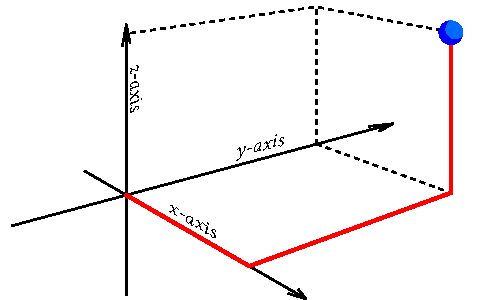
\includegraphics{01xyz-axes.pdf}
  \caption{To determine the location of points in three dimensional
    space (such as the center of the blue sphere in this drawing), we
    should choose three coordinate axes, and specify three numbers:
    the $x$, $y$, and $z$ coordinates of the point.  }
\end{figure}

\subsection{Vectors}  
While points and their coordinates are used to described locations in space,
vectors are used to describe \emph{displacements}, i.e.~how to go from one point
to another.  Such a displacement has a size (how far we have to go), and a
direction (which way do we go).  Vectors also get used in non-geometric
situations to describe objects that have size and direction, e.g.~velocities and
forces in physics are typical examples of vector-like objects.

\subsubsection*{Informal definition of ``vectors''}
We will think of a vector as an arrow connecting two points.  If the points are
$A$ and $B$ then we call the vector $\tpv AB$. If we translate a vector $\tpv
AB$ \emph{without turning it} then we say that the resulting vector $\tpv CD$ is
the same vector as the original vector $\tpv AB$.  A more precise way  of saying
that we should be able to move $\tpv AB$ ``without turning,'' is to insist that
the line segments $AB$ and $CD$ should be parallel, and have the same length and
orientation.

\begin{figure}[h]\centering
  \input ../figures/234/005equalvectors.tex
  \caption{This figure contains \emph{four} points ($A$, $B$, $C$, $D$),
  \emph{two} line segments ($AB$ and $CD$), but \emph{only one} vector since
  $\tpv AB$ and $\tpv CD$ represent the same vector:  $\tpv AB = \tpv CD$.}
\end{figure}
We say that the arrows $\tpv AB$ and $\tpv PQ$ \emph{both represent the same
vector.}  Since both $\tpv AB$ and $\tpv PQ$ are the same vector we will often
want to use a notation for vectors that does not emphasize any particular choice
of initial-~and endpoint.  The notation we will use in this course is
\[
\va = \tpv AB = \tpv PQ,
\]
i.e., a single letter with an arrow on top will always stand for a
vector in this course.

\begin{figure}[h]\centering
  \def\figfont{\sffamily\footnotesize\color{darkbluegreen}\centering}
  \def\addingvectorsCapA{\parbox{1in}{\figfont%
      to add\\
      two vectors\dots}} \def\addingvectorsCapB{\parbox{1in}{\figfont%
      \dots move one vector until its initial point\dots}}
  \def\addingvectorsCapC{\parbox{1in}{\figfont%
      \dots is the end point of the other\dots} }
  \def\addingvectorsCapD{\parbox{1in}{\figfont%
      \dots and combine them.} } \input
  ../figures/234/005adding-vectors2.pdf_tex
  \caption{Adding vectors}
\end{figure}
\section{Arithmetic of vectors}  
\label{sec:arithmetic-of-vectors}
To add two vectors $\tpv AB$ and $\tpv PQ$ we first translate the vector $\tpv
PQ$ so that its initial point becomes $B$; let the result of this translation be
the vector $\tpv BC$.  Then, by definition, the sum of $\tpv AB$ and $\tpv PQ$
is $\tpv AC$: in a formula,
\[
\tpv AB + \tpv PQ = \tpv AB + \tpv BC = \tpv AC.
\]
An equivalent way of adding two vectors $\tpv AB$ and $\tpv PQ$ is to move the
vectors around until they have the same initial point.  Two vectors with a
common initial point form two sides of a parallelogram (see
Figure~\ref{fig:adding-vectors-parallelogram}) and the sum of the two vectors is
the diagonal of that parallelogram.
\begin{figure}[h]
  \input ../figures/234/005adding-vectors-parallelogram.pdf_tex
  \caption{{\bfseries Using a parallelogram to add vectors. } To find $\tpv AB +
  \tpv AD$ we move the vector $\tpv AD$ so that its initial point is at $B$,
  i.e.~the endpoint of $\tpv AB$.  This gives us a parallelogram $ABCD$, where
  $\tpv AD = \tpv BC$.  Therefore $\tpv AB+\tpv AD = \tpv AB+\tpv BC = \tpv AC$
  }
  \label{fig:adding-vectors-parallelogram}
\end{figure}

One can also multiply vectors with numbers.  To multiply a vector $\va$ with a
positive real number $t>0$, we multiply the length of the vector by a factor
$t$, without changing the direction of the vector.
\begin{figure}[h]
  \input ../figures/222/05scalar-mult.pdf_tex
  \caption{Multiplying and subtracting vectors}
\end{figure}
\section{Vector algebra}  
The addition and multiplication of vectors and numbers satisfy a number of
algebraic properties that should look familiar, as they are very similar to the
usual algebraic properties for adding and multiplying numbers.  Here they are:
\begin{align*}
  \va+\vb&=\vb+\va &&& \text{commutative law}\\
  (\va+\vb)+\vc &= \va+(\vb+\vc) & t\cdot(s\cdot\va) &= (ts)\cdot \va
  &\text{associative laws}\\
  t\cdot(\va+\vb) & = t\va+t\vb & (t+s)\va &= t\va + s\va
  &\text{distributive laws}
\end{align*}
\section{Component representation of vectors}  
\label{sec:component-rep-of-vectors}

\subsection{Components of a vector in two dimensional space}  
\label{sec:comp-vect-two}
There is a way to represent a vector by specifying a list of numbers instead of
by giving a geometric description of the vector.  To do this for vectors in the
plane, we must choose two perpendicular coordinate axes (the ``$x$'' and ``$y$''
axes).  We define
\begin{align*}
  \ves1 &= \text{ vector with length $1$, in the direction of the $x$ axis} \\
  \ves2 &= \text{ vector with length $1$, in the direction of the $y$ axis}
\end{align*}
Then any other vector can be written as the sum of a multiple of $\ves1$ and
another multiple of $\ves2$:
\begin{equation}
  \va = a_1\ves1 + a_2 \ves2.
  \label{eq:vector-a-in-components}
\end{equation}
See Figure~\ref{fig:vector-in-components}.  The numbers $a_1$ and $a_2$ are
called the \emph{components of the vector $\va$.}  If we know the components
$a_1$ and $a_2$ of a vector, and if we know the two vectors $\ves1$ and $\ves2$,
then we can reconstruct the vector $\va$ by using the formula
\eqref{eq:vector-a-in-components}.

\begin{figure}[h]
  \input{../figures/234/005vector-components.pdf_tex}
  \caption{Describing a vector in terms of its components.}
  \label{fig:vector-in-components}
\end{figure}

Instead of using the notation \eqref{eq:vector-a-in-components}, one very often
writes
\begin{equation}
  \va = \vek a_1 \\ a_2 \tor,
  \text{ or }
  \va = \begin{bmatrix}
    a_1 \\ a_2
  \end{bmatrix}, \text{ or } \va = \langle a_1, a_2\rangle.
  \label{eq:vector-a-as-column-vector}
\end{equation}
This notation says that $\va$ is the vector whose components are $a_1$ and
$a_2$.  Since the two vectors $\ves1$ and $\ves2$ depend on our choice of
coordinate axes, we can only use the component notation if it is clear to
everyone how we chose the coordinate axes.

The first way of writing the vector, in which the components $a_1$ and $a_2$ are
listed in a column enclosed in either parentheses or square brackets, is the
standard way of writing ``column vectors,'' and is used in linear algebra
courses (math 320, 340, 341, etc.), as well as by most computational software
(Matlab$^{\rm TM}$, Octave, etc.).  The other way of writing the components,
i.e.~as $\langle a_1, a_2\rangle$, also
gets used, especially when one has to type the equations rather than write them
by hand.

\subsection{Components of a vector in three dimensional space}  
\label{sec:comp-vect-three}
The preceding also applies to vectors in three dimensional space: instead of
choosing two coordinate axes we choose three axes, and call them the $x$, $y$,
and $z$ axes (or, the $x_{1}$, $x_{2}$, and $x_{3}$ axes).  Then we define
$\vi$, $\vj $, and $\vk$ (or $\ves1$, $\ves2$, and $\ves3$) to be vectors of
length one in the direction of the three coordinate axes.  A vector $\va$ in
space can then be written as a combination of the three vectors $\vi$, $\vj$,
and $\vk$, namely,
\[
 \va = a_{1}\vi + a_2 \vj + a_3 \vk, \text{ or }
 \va = \vek a_1\\a_2\\a_3 \tor.
\]
\begin{figure}[h]
  \sffamily\color{darkbluegreen}
  \input{../figures/234/005vector-components3D.pdf_tex}
  \caption{Components of a vector in three dimensional space}
  \label{fig:vector-in-components-3d}
\end{figure}%
\marginpar{\centering\dfnt Josiah Willard Gibbs\\
1839--1903\\[2pt]
%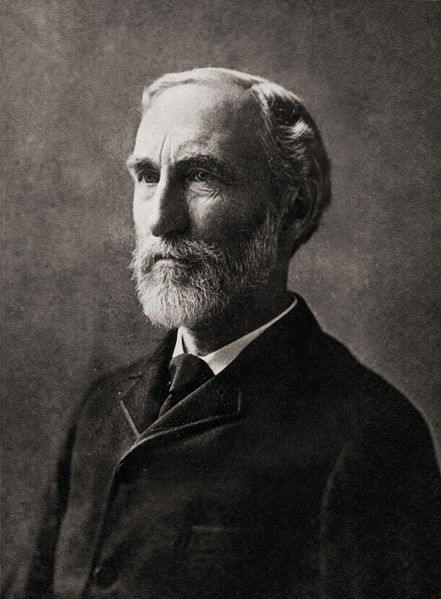
\includegraphics[width=1in]{Josiah_Willard_Gibbs.jpg}\\
\tiny\url{https://en.wikipedia.org/wiki/Josiah_Willard_Gibbs}}%
The $\ves1$, $\ves2$, $\ves3$ notation is more systematic, but the $\vi$, $\vj$,
$\vk$ notation, which was introduced into vector geometry and vector calculus by
J.W.Gibbs, is also very common.

\subsection{Length of a vector whose components are given}  
\label{sec:length-vector-given-components}
We will write
\[
\|\va\|
\]
for the length of a vector $\va$.  If the vector is given in components, 
\[
  \va = a_1\ves1+a_2\ves2, 
  \text{ or }
  \va = a_1\ves1+a_2\ves2+a_3\ves3, 
\]
then the length of the vector is determined by Pythagoras' law (see
Figures~\ref{fig:vector-in-components} and~\ref{fig:vector-in-components-3d}):
\begin{equation}
  \|\va\| = \sqrt{a_1^2 + a_2^2}, \quad
  \text{ or }\quad
  \|\va\| = \sqrt{a_1^2 + a_2^2+a_3^2}. 
  \label{eq:length-of-vector-from-components}
\end{equation}



\section{The dot product}  
There are two different descriptions of the dot product of two
vectors: one geometric, and the other in terms of the components of
the vectors.

\subsection{Geometric description of the dot product}  
If $\va$ and $\vb$ are two given vectors, then, by definition,
\marginpar{\footnotesize\sffamily\centering\color{darkbluegreen}%
  \input ../figures/234/005dot-product.pdf_tex

  The dot product between two vectors.
}
\begin{equation}
  \label{eq:dotproduct-geometric}
  \va\dpp\vb = \|\va\| \, \|\vb\|\,\cos \theta,
\end{equation}
where $\theta$ is the angle between the two vectors $\va$ and $\vb$.

\subsection{The dot product in terms of vector components}  
If we choose an orthonormal set of vectors $\ves1,\ves2,\ves3$, and write
\[
  \va = a_1\ves1+a_2\ves2+a_3\ves3=\vek a_1 \\ a_2 \\ a_3 \tor,\qquad
  \vb = b_1\ves1+b_2\ves2+b_3\ves3=\vek b_1 \\ b_2 \\ b_3 \tor,
\]
then
\begin{equation}
  \label{eq:dotproduct-algebraic}
  \va\dpp\vb = a_1b_1 + a_2b_2 + a_3b_3.
\end{equation}
The fact that \eqref{eq:dotproduct-geometric} and \eqref{eq:dotproduct-algebraic}
always give the same result is not obvious (the formulas look very different), and
requires a proof.  A very common proof relies on the law of cosines (it was given in math 222 -- see also Problem~\ref{prb:law-of-cosines-and-dotprod})

\subsection{Algebraic properties of the dot product}  
\label{sec:dotproduct-algebraic-properties}%
The dot product has the following algebraic properties, which we will
use very often throughout this course:
\begin{align*}
  \va\dpp\vb &= \vb\dpp\va & \text{commutative} \\
  s(\va\dpp\vb) &= (s\va)\dpp\vb & \text{associative} \\
  (\va+\vb)\dpp\vc & = \va\dpp\vc + \vb\dpp\vc. & \text{distributive}
\end{align*}
We will not prove these properties here.  Proofs can be given if one
starts either from the algebraic description of the dot-product
\eqref{eq:dotproduct-algebraic}, or from the geometric description
\eqref{eq:dotproduct-geometric} (although the distributive property is
more difficult to prove from the geometric description than from the
algebraic description.)

The sign of the dot product tells us if the angle between two vectors is acute,
obtuse, or if the vectors are perpendicular:
\begin{subequations}
  \begin{align}
    \va\perp\vb  &\iff \va\dpp\vb=0 \\
    \va\dpp\vb>0 &\iff \theta<\frac{\pi}{2}\\
    \va\dpp\vb<0 &\iff \theta>\frac{\pi}{2}.
  \end{align}
\end{subequations}

\section{The cross product}  
As with the dot product, the cross product of two vectors also has a
geometric description, and a description in terms of components.

\subsection{Geometric description of the cross product} Let $\va$  
and $\vb$ be two vectors in three dimensional space, then their
\emph{cross product} is the vector $\va\cp\vb$ that satisfies
\begin{itemize}
\item $\va\cp\vb$ is perpendicular to $\va$, and also to $\vb$
\item the length of $\va\cp\vb$ is given by
  \[
  \|\va\cp\vb\| = \|\va\|\,\|\vb\|\,\sin\theta,
  \]
  where $\theta$ is the angle between the vectors $\va$ and $\vb$,
\item the three vectors $\va$, $\vb$, $\va\cp\vb$ satisfy the
  \emph{right hand rule:} if on your right hand $\va$ is the index
  finger and $\vb$ is the middle finger, then your thumb points in the
  direction of $\va\cp\vb$.  See Figure~\ref{fig:cross-product}.
\end{itemize}
\begin{figure}[t]
  \input ../figures/222/05crossprod-corkscrew.pdf_tex
  \caption{The cross product: $\va\cp\vb$ is perpendicular to both
    $\va$ and $\vb$; its direction follows from the right-hand rule. }
  \label{fig:cross-product}
\end{figure}
The length of the cross product of two vectors has a geometric
interpretation.  Namely, the quantity $\|\va\|\,\|\vb\|\,\sin\theta$
is exactly the are of the parallelogram spanned by the vectors $\va$
and $\vb$.
\begin{figure}[h]
  \input
  ../figures/222/05area-parallelogram-spanned-by-vectors.pdf_tex
\end{figure}

\subsection{Algebraic description of the cross product} If $\va$  
and $\vb $ are given by \eqref{eq:dotproduct-geometric}, i.e.~by
\[
\va = a_1\ves1+a_2\ves2+a_3\ves3=\tvek a_1 \\ a_2 \\ a_3 \ttor,\qquad
\vb = b_1\ves1+b_2\ves2+b_3\ves3=\tvek b_1 \\ b_2 \\ b_3 \ttor,
\]
then
\[
\va \cp\vb = \vek
a_2b_3 - a_3b_2\\
a_3b_1 - a_1b_3\\
a_1b_2 - a_2b_1\tor.
\]

\subsection{Algebraic properties of the cross product}  
\label{sec:cross-product-algebraic-properties}
The cross product has the distributive property, namely,
\begin{equation}
  (\va+\vb)\cp\vc  = \va\cp\vc + \vb\cp\vc,
  \label{eq:cross-product-distributive}
\end{equation}
holds true for any three vectors $\va$, $\vb$, $\vc$.

The cross product is \emph{not commutative}: $\va\cp\vb$ and
$\vb\cp\va$ are not the same thing.  Instead, we have :
\begin{equation}
  \va\cp\vb = -\vb\cp\va.
\end{equation}
Because of this property the cross product is said to be
``\textit{anti-commutative.}''

The associative property fails completely for the cross product: for
most vectors $\va$, $\vb$, $\vc$ one has
\begin{equation}\color{red}
  \carefulnow\carefulnow\qquad
  (\va\cp\vb)\cp\vc\; {\boldsymbol \neq}\; \va\cp(\vb\cp\vc)
  \qquad \carefulnow\carefulnow
  \label{eq:cross-product-not-associative}
\end{equation}

If you need a vector that is perpendicular to two given vectors, take
their cross product.

The length of the cross product $\va\cp\vb$ is the area of the
parallelogram spanned by those vectors.

\section{The triple product}  
\label{sec:determ-triple-prod}
Just as two vectors in the plane form a parallelogram, three vectors
in space will form a shape called a parallelepiped.  By definition, a
parallelepiped is a solid body each of whose faces is a parallelogram.

\begin{figure}[h]
  \def\svgwidth{200pt}
  \input ../figures/234/01parallelepiped.pdf_tex\hfill
  \def\svgwidth{130pt}
  \input ../figures/234/01parallelepiped-flipped.pdf_tex
  \caption{\textbf{A parallelepiped spanned by three vectors $\va$,
      $\vb$, $\vc$.}  Since the base of the parallelepiped is a
    parallelogram with edges $\vb$ and $\vc$, we have \\
    \null\qquad Area of base~$= \|\vb\cp\vc\|$.\\
    The height of the parallelepiped is $\|\va\|\cos\theta$, and
    therefore the volume is given by \\
    \null\qquad Volume = $\text{height}\cdot\text{area of base}
    = \|\va\| \, \|\vb\cp\vc\| \cos\theta
    = \va\dpp\bigl(\vb\cp\vc\bigr)$.\\
    This derivation applies to the situation on the left, where the
    vector $\va$ and the cross product $\vb\cp\vc$ point in the same
    direction.  If these vectors form an obtuse angle, as is the case
    on the right, then $\cos\theta<0$, and the height is
    $-\|\va\|\cos\theta$.  In that case one has\\
    \null\qquad Volume = $\text{height}\cdot\text{area of base}
    = - \|\va\| \, \|\vb\cp\vc\| \cos\theta 
    = - \va\dpp\bigl(\vb\cp\vc\bigr)$.
  }
  \label{fig:volume-of-parallelpiped}
\end{figure}
If we are given three vectors $\va$, $\vb$, and $\vc$, then the volume
of the parallelepiped they determine is given by the formula
\[
\text{``Volume equals Area of base times height''}
\]
In terms of the three vectors this is
\begin{equation}
  V = \left| \va\dpp\bigl(\vb\cp\vc\bigr)\right|.
  \label{eq:volume-of-parallelpiped}
\end{equation}
A derivation is sketched in Figure~\ref{fig:volume-of-parallelpiped}.
The quantity $\va\dpp(\vb\cp\vc)$ (without the absolute values) is
called the \emph{triple product} of the three vectors $\va$, $\vb$,
and $\vc$.  Apart from its use in computing the volume of a
parallelepiped, the triple product appears in many other contexts.  At
first sight the expression $\va\dpp(\vb\cp\vc)$ suggests that the
order in which the vectors appear is important, but this turns out not
to be true.  One has 
\[
\va\dpp\bigl(\vb\cp\vc\bigr) = \vb\dpp\bigl(\vc\cp\va\bigr) =
\vc\dpp\bigl(\va\cp\vb\bigr)
\]
for any $\va,\vb,\vc$.

\section{Determinants}  
\label{sec:determinants}
For any four numbers $a$, $b$, $c$, $d$, one defines the $2\times2$
determinant to be
\begin{equation}
  \deter a&b \\ c& d
  \minant
  =ad-bc\,.
  \label{eq:determinant-2x2}
\end{equation}
One can also define $3\times3$ determinants.  Namely, for any nine
numbers $a_1, \dots, c_3$ one defines
\begin{equation}
  \deter
      a_1 & b_1 & c_1 \\
      a_2 & b_2 & c_2 \\
      a_3 & b_3 & c_3
  \minant
  =
  a_1b_2c_3 - a_1b_3c_2 - a_2b_1c_3 + a_2b_3c_1 +a_3b_1c_2 - a_3b_2c_1\,.
  \label{eq:triple-product}
\end{equation}
This can be written as
\begin{align}
  \deter
  \color{red}a_1 & b_1 & c_1 \\
  \color{red}a_2 & b_2 & c_2 \\
  \color{red}a_3 & b_3 & c_3
  \minant
  &={\color{red}a_1}\bigl(b_2c_3-b_3c_2\bigr)
  - {\color{red}a_2}\bigl(b_1c_3-b_3c_1\bigr)
  + {\color{red}a_3}\bigl(b_1c_2-b_2c_1\bigr)
  \label{eq:determinant-expanded-along-column}
  \\
  &= {\color{red}a_1} \deter b_2 & c_2 \\ b_3 & c_3 \minant
  - {\color{red}a_2} \deter b_1 & c_1 \\ b_3 & c_3 \minant
  + {\color{red}a_3} \deter b_1 & b_1 \\ b_2 & b_2 \minant
  \notag
\end{align}
where each coefficient in the first row is multiplied with the
$2\times2$ determined that remains after one deletes the row and
column containing the coefficient.

Instead of expanding along the first row one can also expand along the
first column:
\begin{equation}
  \deter
  \color{red}a_1 & \color{red}b_1 & \color{red}c_1 \\
  a_2 & b_2 & c_2 \\
  a_3 & b_3 & c_3
  \minant
  = {\color{red}a_1}\deter b_2 & c_2 \\ b_3 & c_3 \minant
  - {\color{red}b_1}\deter a_2 & c_2 \\ a_3 & c_3 \minant
  + {\color{red}c_1}\deter a_2 & b_2 \\ a_3 & b_3 \minant
  \label{eq:determinant-expanded-along-row}
\end{equation}
Many other mnemonic devices exist to remember how to compute a
$3\times3$ determinant.  A popular trick is ``Sarrus' rule'' (see
Figure~\ref{fig:Sarrus}.)

One can also define larger determinants, i.e.~$4\times4$, $5\times5$,
etc, and generally $n\times n$ determinants.  The theory, which is
beyond the scope of this course, is treated in linear algebra courses
such as Math 320, 340, or 341.

\section{Determinants, the triple product, and the cross product}  
\label{sec:determ-triple-prod-cross-prod}
If the numbers $a_1, \dots, c_3$ in a determinant happen to be the
components of three vectors $\va$, $\vb$, $\vc$, i.e.~if
\[
\va = \vek a_1\\ a_2 \\a_3\tor, \vb = \vek b_1\\ b_2 \\b_3\tor, \vc =
\vek c_1\\ c_2 \\c_3\tor,
\]
then the corresponding determinant is exactly the triple product:
\begin{equation}
  \left|
    \begin{array}{ccc}
      a_1 & b_1 & c_1 \\
      a_2 & b_2 & c_2 \\
      a_3 & b_3 & c_3
    \end{array}
  \right|= \va\dpp\bigl(\vb\cp\vc\bigr).
\end{equation}%
\begin{figure}[t]
  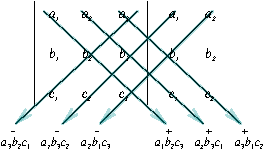
\includegraphics[scale=1.30]{05determinant-shortcut2.pdf}
  \caption{\textbf{Computing $3\times3$ determinants. } There are several
    shortcuts to remember how to compute a $3\times3$ determinant.
    Pictured here is ``Sarrus' rule,'' which tells us to copy the
    first two columns of the determinant to the right of the
    determinant, and read off the six terms in the determinant by
    following the diagonals. }
  \label{fig:Sarrus}
\end{figure}%
Related to this is the following practical trick for computing the
cross product of two column vectors.  Given two column vectors $\vb$
and $\vc$ one can write their cross product as 
\begin{align*}
  \vek b_1\\b_2\\b_3\tor\cp \vek c_1\\c_2\\c_3\tor
  &=
  \deter
  \ves1 & b_1 & c_1 \\
  \ves2 & b_2 & c_2 \\
  \ves3 & b_3 & c_3
  \minant \\
  &=  \deter b_2 & c_2 \\ b_3 & c_3 \minant \ves1
    - \deter b_1 & c_1 \\ b_3 & c_3 \minant \ves2
    + \deter b_1 & c_1 \\ b_2 & c_2 \minant \ves3 .
\end{align*}
The $3\times3$ determinant in this equation is unusual in that some of its
entries are vectors instead of numbers.  The intention of this notation is that
one expand the determinant along the first column, as in
\eqref{eq:determinant-expanded-along-column} and then interpret the result as a
vector.

\section{Defining equations for lines and planes}  
\label{sec:defining-equations-lines-and-planes}
\subsection{Lines}  
\label{sec:defining-eq-lines}
Let $\ell$ be a line in the plane, and suppose we know one point $A$ on the
line, and that we also have a vector $\vn$ that is perpendicular to the line
(and we exclude $\vn=\vvv0$.) Such a vector is called a \emph{normal vector} to
the line.  Given any other point $X$ in the plane we can form the vector $\tpv
AX$ and consider its dot-product with the normal.  We have
\[
  \vn \dpp \tpv AX = \|\vn\| \, \|\tpv AX\| \cos \theta,
\]
where $\theta$ is the angle between the normal vector $\vn$ and $\tpv AX$.

\begin{figure}[h]
  \hspace{-1em}\input ../figures/222/05distance-to-line.pdf_tex
\end{figure}
The combination $\|\tpv AX\|\cos \theta$ is, up to its sign, the distance from
the line $\ell$ to the point $X$: If $X$ lies on the side of $\ell$ at which the
normal vector points then $\vn\dpp\tpv AX>0$; if $X$ lies on the other side then
$\vn\dpp\tpv AX<0$.  We therefore have the following formula for \textit{the
distance between a point $X$ and the line $\ell$:}
\begin{equation}
  d = \frac{\vn \dpp \tpv AX	}{\|\vn\|}
  \label{eq:distance-to-line}
\end{equation}
When we use this equation to compute the distance from $X$ to $\ell$, it is good
to recall that if $\vx=\tvek x_1\\x_2\ttor$ and $\va = \tvek a_1\\ a_2\ttor$ are
the position vectors of the points $X$ and $A$, then  
\[
  \tpv AX = \vx-\va = \vek x_1-a_1 \\ x_2-a_2\tor.
\]
Moreover, the length of the normal vector is $\|\vn\| = \sqrt{n_1^2+n_2^2}$, so
we can rewrite \eqref{eq:distance-to-line} as 
\[
  d = \frac{n_1(x_1-a_1) + n_2(x_2-a_2)}{\sqrt{n_1^2 + n_2^2}}.
\]
This last formula is more impressive than \eqref{eq:distance-to-line}, but it is
better to remember \eqref{eq:distance-to-line}.

The equation for the distance from any point $X$ to a given line $\ell$ is also
important because it gives us \emph{the defining equation} for the line $\ell$.
The defining equation is an equation that tells us for any given point $X$ in
the plane if that point is on the line or not.  Since $X$ is on $\ell$ exactly
when the distance from $\ell$ to $X$ vanishes, it follows from
\eqref{eq:distance-to-line} that $X$ is on $\ell$ if and only if 
\begin{equation}
  \vn\dpp\tpv AX = 0.
  \label{eq:defining-eqn-for-line}
\end{equation}
We can again rewrite this equation in a few different ways.  If we want to write
it in terms of the position vectors of $A$ and $X$, then we get
\[
  \vn \dpp \bigl(\vx-\va\bigr) = 0, \qquad
  \text{ i.e.: }\qquad
  \vn\dpp\vx = \vn\dpp\va.
\]
Written without vectors, but in terms of the coordinates of the points $A$,
$X$, and the components of the normal vector $\vn$, we can write this last
version of our equation as
\[
  n_1x_1+n_2x_2 = n_1a_1+n_2a_2.
\]

\subsection{Planes}  
\label{sec:defining-eq-planes}
We can repeat the derivation of the distance from a point to a line in
the plane and derive a formula for the distance from a point in three
dimensional space to a given plane.  The drawings are harder to make
(at first only, practice makes perfect!), but the resulting formulas
are the same.
\begin{figure}[h]
  \centering
  \input ../figures/234/01distance-to-plane.pdf_tex
\end{figure}

The distance from a point $X$ to a plane $\cP$ is given by equation
\eqref{eq:distance-to-line}, where $\vn$ is a normal vector to the
plane (a vector that is perpendicular to the plane), and $A$ is some
point on the plane that we happen to know.


\section{Problems}  
\begin{multicols}{2}
\problemfont  
\problem \subprob Simplify the following 
\begin{align*}
  \va &= \vek 1\\-2\\3 \tor + 3\vek 0 \\ 1 \\3 \tor \\
  \vb &=  12\vek 1 \\ 1/3\tor - 3\vek 4 \\ 1\tor \\
  \vc &= (1+t)\vek 1 \\ 1-t\tor - t\vek 1 \\ -t\tor \\
  \vd &= t\vek1\\0\\0\tor + t^2\vek0\\-1\\2\tor-\vek0\\0\\1\tor
\end{align*}
\subprob Write the vectors from part \textbf{(a)} using Gibbs' notation, i.e.~write
them in terms of $\vi$, $\vj$, $\vk$.   (See \S~\ref{sec:component-rep-of-vectors}).

\problem If $\va,\vb, \vc$ are as in the previous problem, then 
which of the following expressions mean anything? Compute those
expressions that are well defined.
\begin{align*}
  \tsubprob& \va+\vb  &\tsubprob& \vb+\vc &\tsubprob& \pi\va \\
  \tsubprob& \vb^2    &\tsubprob& \vb/\vc &\tsubprob& \nm\va+\nm\vb \\
  \tsubprob& \nm\vb^2 &\tsubprob& \vb/\nm\vc &&
\end{align*}

\problem Let $\va=\tvek1\\-2\\2\ttor$ and $\vb=\tvek 2\\-1\\1\ttor$.
\quad Compute:
\begin{align*}
&\tsubprob ||\va||&&
\tsubprob 2\va&&
\tsubprob ||2\va||^2\\
&\tsubprob \va+\vb&&
\tsubprob 3\va-\vb&&
\end{align*}
\vskip-2ex
\answer  
(a) $3$ \quad
(b) $\tvek 2\\ -4\\ 4\ttor$  \quad
(c) 36  \quad
(d) $\tvek 3\\ -3\\ 3\ttor$  \quad
(e) $\tvek 1\\ -5\\ 5\ttor$
\endanswer

\problem Given: points $A (2,1)$ and $B (-1,4)$.  Compute the vector $\tpv AB$.
\textit{Is $\tpv AB$ a position vector?}
\answer 
Every vector is a position vector.  To see of which point it is the position
vector translate it so its initial point is the origin.

Here $\tpv AB = \vek -3\\ 3 \tor$, so $\tpv AB$ is the position vector of
the point $(-3,3)$.
\endanswer

\problem Given: points $A (2,1)$, $B (3,2)$, $C (4,4)$ and $D (5,2)$.\\
Question: \textit{Is $ABCD$ a parallelogram?}
\answer 
One always labels the vertices of a parallelogram counterclockwise (see
\S\ref{sec:diag-parall}). 

$ABCD$ is a parallelogram if $\tpv AB + \tpv AD = \tpv AC$.  
$\tpv AB = \vek 1\\ 1 \tor$, $\tpv AC = \vek 2\\ 3 \tor$, $\tpv AD = \vek 3\\
1 \tor$.  So $\tpv AB + \tpv AD \ne \tpv AC$, and $ABCD$ is not a
parallelogram.
\endanswer

\problem Given: points $A (0,2,1)$, $B (0,3,2)$, $C (4,1,4)$ and $D$.

\subprob If $ABCD$ is a parallelogram, then what are the coordinates of
the point $D$?
\answer 
As in the previous problem, we want $\tpv AB + \tpv AD = \tpv AC$.
If $D$ is the point $(d_1, d_2, d_3)$ then 
$\tpv AB = \vek 0\\ 1\\1 \tor$, 
$\tpv AD = \vek d_1\\ d_2-2 \\ d_3-1\tor$,
$\tpv AC = \vek 4\\ -1\\ 3 \tor$,
so that $\tpv AB + \tpv AD = \tpv AC$ will hold if 
$d_1 = 4$, $d_2 = 0$ and $d_3 = 3$.
\endanswer

\subprob If $ABDC$ is a parallelogram, then what are the coordinates of
the point $D$?
\answer 
Now we want $\tpv AB + \tpv AC = \tpv AD$, so $d_1 = 4$, $d_2 = 2$,
$d_3 = 5$.
\endanswer

\problem You are given three points in the plane: $A$ has coordinates $(2,3)$, $B$
has coordinates $(-1,2)$ and $C$ has coordinates $(4,-1)$.

\subprob Compute the vectors $\tpv AB$, $\tpv BA$, $\tpv AC$, $\tpv CA$, $\tpv
BC$ and $\tpv CB$.

\subprob Find the points $P, Q, R$ and $S$ whose position vectors are $\tpv AB$,
$\tpv BA$, $\tpv AC$, and $\tpv BC$, respectively.  \textit{Make a precise
drawing.}

\problem Explain how you can use the dot product to find the angle  
between the vectors $\va = 2\vi-3\vj$, and $\vb=\vj+\vk$.

\problem For which value(s) of the number $s$ are the vectors  
\[
\va =\vek s \\1-s\tor \text{ and }
\vb = \vek 2\\3\tor
\]
perpendicular?  For which values of $s$ do they make an acute angle?
\answer  
Compute the dot product: $\va\dpp\vb = 2s+3(1-s) = 3-s$.  When the
dot-product vanishes the vectors are perpendicular; this happens when
$s=3$.  The angle between the vectors is acute is the dot-product is
positive.  This happens when $3-s>0$, i.e.~when $s<3$.
\endanswer

\problem\label{prb:cube-planes-angles} Figure  
\ref{fig:cube-planes-angles} shows a cube whose sides have length 1.

Choose $A$ to be the origin, and let the $x$, $y$, and $z$ axes be
along the sides $AB$, $AD$, and $AE$, respectively.

\subprob Draw the vectors $\ves1$, $\ves2$, and $\ves3$ in the figure.  

\subprob Find a normal vector to the plane through the points $B$,  
$D$, and $E$.

\subprob Draw the plane through $ACH$ (or at least the portion of that  
plane that lies inside the cube).  Find a normal to the plane $ACH$.

\subprob Find the angle between the two planes $BDE$ and $ACH$.  
(The angle between two planes is the same as the angle between their normal
vectors, i.e.~to find the angle between two planes find a normal vector for each
of the planes and compute the angle between these two vectors.)

\subprob Find the angle between the two planes $BDE$ and $HFC$.  

\problem \subprob Draw two vectors $\va$ and $\vb$ for which  
$\va$ has length 3, $\vb$ has length $5$, and for which $\va\dpp\vb=-12$.
How many solutions are there?%
\answer  
The problem is open-ended because it doesn't specify what ``draw'' means.

If you are allowed to use a calculator and a protractor, then you could use the
dot product to compute the angle $\theta$ between the two vectors; then, using
your protractor, draw two line segments that make this angle, and mark off
lengths 3 and 5 to get the vectors.  From the dot-product and the two lengths
you find $3\times5\times\cos\theta = -12$, so $\cos\theta = - \frac{12}{15}=
-0.8$, which implies $\theta = \arccos (-0.8) \approx 2.498\dots$ radians, or
$\theta\approx 143.13\dots$ degrees.

A different approach goes like this.  Suppose $\va$ is parallel to the $x_1$ axis; since $\va$ has length $3$, we can choose $\va=3\ves1$.  Now we look for a matching vector $\vb=\tvek b_1\\b_2\ttor$.  The condition that $\vb$ must have length 5
then says $b_1^2 + b_2^2 = 5^2 = 25$, while the dot-product is $\va\dpp\vb =
a_1b_1+a_2b_2 = 3b_1$.  Since the dot-product must be $-12$ we find
$b_1=-\frac{12}{3}=-4$.  Using the length of $\vb$ leads to
$b_2=\sqrt{25-(-4)^2} = \pm3$.  Thus we find two solutions: $\vb = \tvek -4\\
\pm3\ttor = -4\ves1\pm3\ves2$.

You make the drawing.
\endanswer

\subprob Can there be two vectors $\va$ and $\vb$ whose lengths are  
$\|\va\| = 3$ and $\|\vb\|=5$, and whose inner product is $\va\dpp\vb = 25$?
\answer  
No.  The inner product of two vectors is $\va\dpp\vb = \|\va\|\,\|\vb\|
\cos\theta$, and therefore it can never be larger than $\|\va\|\,\|\vb\|$.
\endanswer

\problem Compute %---Is the cross product associative?
\[
  \va = (\vi\cp\vj)\cp\vj \quad \text{ and }\quad 
  \vb = \vi\cp(\vj\cp\vj).
\]
What does your answer say about the associative property for the cross product?
(See \S~\ref{sec:cross-product-algebraic-properties}.)

What about
\[
  \vc = (\vi\cp\vj)\cp\vk \quad \text{ and }\quad 
  \vd = \vi\cp(\vj\cp\vk)?
\]

\problem Which of the following vector equations are true for any pair  
of vectors $\va$ and $\vb$?  Either give a proof (using the algebraic
properties or the algebraic or geometric descriptions).

\subprob $(\va+\vb)\dpp(\va-\vb) = \|\va\|^2 - \|\vb\|^2$~?  
\answer  
True:
\begin{align*}
  (\va+\vb)\dpp(\va-\vb) &=(\va+\vb) \dpp \va  - (\va+\vb) \dpp\vb\\
  &= \va \dpp \va +\vb \dpp \va  - \va \dpp\vb - \vb \dpp\vb\\
  &= \|\va\|^2 + \| \vb \|^2.
\end{align*}
\endanswer

\subprob  If  $\va\perp\vb$ then\\[1ex] 
\null\hfill$\|\va+\vb\|^2 = \|\va\|^2 + \|\vb\|^2$~?% 
\answer  
True:  This is Pythagoras' theorem.  Here is an algebraic derivation:
\begin{align*}
  \|\va+\vb\|^2 &= (\va+\vb) \dpp (\va+\vb)\\
  &= (\va+\vb) \dpp \va  + (\va+\vb) \dpp\vb\\
  &= \va \dpp \va +\vb \dpp \va  + \va \dpp\vb + \vb \dpp\vb\\
  &= \|\va\|^2 + 2 \va \dpp\vb + \| \vb \|^2\\
  &= \|\va\|^2 + \| \vb \|^2.
\end{align*}
\endanswer

\subprob If  $\va\perp\vb$ then\\[1ex] 
\null\hfill$\|\va-\vb\|^2 = \|\va\|^2 - \|\vb\|^2$  ~?%
\answer  
Not so.
The same computation as for the previous problem shows
\begin{align*}
  \|\va - \vb\|^2 &= (\va-\vb) \dpp (\va-\vb)\\
  &= (\va-\vb) \dpp \va  - (\va-\vb) \dpp\vb\\
  &= \va \dpp \va -\vb \dpp \va  - \va \dpp\vb + \vb \dpp\vb\\
  &= \|\va\|^2 - 2 \va \dpp\vb + \| \vb \|^2\\
  &= \|\va\|^2 + \| \vb \|^2.
\end{align*}
Therefore
\[
\|\va-\vb\|^2 = \|\va\|^2 - \|\vb\|^2
\]
only is true if $\vb=\vvv0$.
\endanswer

%%\problem ``Cramer's rule.''  Suppose we have to find solutions $x$,
%%$y$, $z$, of the following linear equations:
%%\begin{align*}
%%  a_1x+b_1y+c_1z & = d_1 \\
%%  a_2x+b_2y+c_2z & = d_2 \\
%%  a_3x+b_3y+c_3z & = d_3
%%\end{align*}
%%
%%\subprob Show that you can write these equations as
%%\[
%%x\va + y\vb + z\vc = \vd
%%\]
%%for certain vectors $\va$, $\vb$, $\vc$, and $\vd$.
%%
%%\subprob Show how you can get a formula for $x$ by taking the dot
%%product of both sides in the equation $x\va + y\vb + z\vc = \vd$ with
%%the vector $\vb\cp\vc$.
%%
%%\subprob How would you get a similar formula for $y$?  Or $z$?

\noproblemfont
\end{multicols}

\begin{figure}[t] 
  \centering
  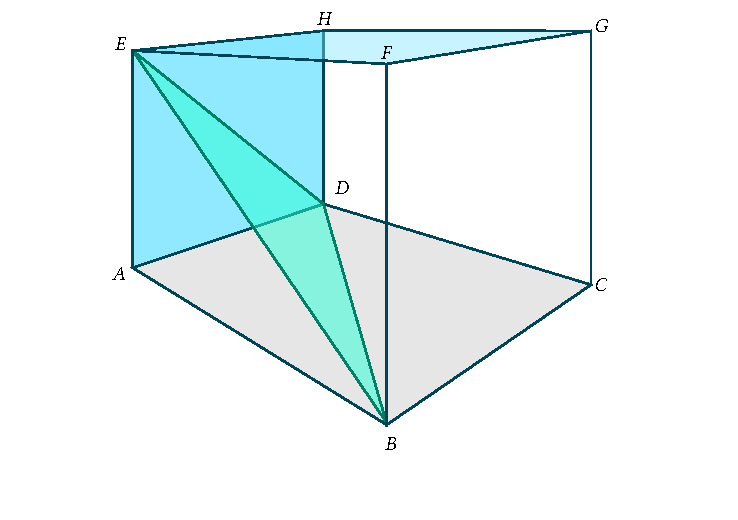
\includegraphics[width=0.75\textwidth]{01problem-cube-planes-angles.pdf}  
  \caption{Figure for problem \ref{prb:cube-planes-angles}}
  \label{fig:cube-planes-angles}  
\end{figure}
%%  TO DO:
%%  Include a story about a salt crystal NaClNaCl...etc.
%%  Do angles between planes show up in spectroscopy?

\begin{multicols}{2}
\problemfont

\problem True or False:  

\subprob If $\va\perp\vb$ and also $\vb\perp\vc$ then $\va\perp\vc$ ?  

\subprob If $\va\perp\vb$ and also $\va\perp\vc$ then $\va\perp(\vb+\vc)$ ?  

\subprob If $\va\perp\vb$ and also $\vb\perp\vc$ then $\vb\perp(\va-\vc)$ ?  

\subprob If $\va\perp\vb+\vc$ and also $\va\perp\vb-\vc$ then $\va\perp\vb$ ?  

\problem Simplify the following expressions  

\subprob \(  (\va+\vb)\cp(\va+\vb) \)  
\answer  
\(  (\va+\vb)\cp(\va+\vb) =\vvv0 \)
\endanswer
%
\subprob \(  (\va+\vb+\vc)\cp(\va+\vb+\vc) \)  
\answer  
\(  (\va+\vb+\vc)\cp(\va+\vb+\vc) =\vvv0 \)
\endanswer
%
\subprob \(  (\va-\vb)\cp(\va+\vb) \)  
\answer  
\(
    (\va+\vb)\cp(\va-\vb) = 2\va\cp\vb.
\)
\endanswer
%
\subprob $(\va+\vb-\vc) \cp (\va-\vb+\vc)$  

\subprob $(\va+\vb-\vc) \dpp (\va-\vb+\vc)$  

\problem  
This problem is about ``cross division,'' i.e.~can you solve
$\va\cp\vb=\vc$ for $\vb$ if you know $\va$ and $\vc$?

\subprob Let  
\begin{equation*}
  \va =\ves1-\ves3,\qquad
  \vc = \ves1+3\ves2+2\ves3.
\end{equation*}
Find a vector $\vb$ for which $\va\cp\vb=\vc$, if there is such a thing.  (Hint:
if $\vc=\va\cp\vb$, then what do you know about $\va\dpp\vc$?)
\answer  
$\va\dpp\vc=\va\dpp(\va\cp\vb) =0$, but for the two given vectors in the problem
$\va\dpp\vc = -1\neq0$, so there cannot be a vector $\vb$ with $\va\cp\vb=\vc$
as $\vc$ is not perpendicular to $\va$.
\endanswer

\subprob Let $\va = 2\ves1-\ves3$, and $\vc = \ves1+3\ves2+2\ves3$.  
Find a vector $\vb$ for which $\va\cp\vb=\vc$, if such a thing exists. %
\answer  
In this case $\va\perp\vc$, so the argument from the first part of this problem
doesn't rule out that there might be a solution.  So let's try $\vb =
\tvek b_1\\b_2\\b_3\ttor$.  Then
\[
  \va\cp\vb
  = \vek b_2 \\ -b_1-2b_3 \\ 2b_2\tor \stackrel?= \vc
  = \vek 1\\3\\2\tor.
\]
Solving this for $b_1$, $b_2$, and $b_3$ leads to $b_2=1$, and $-b_1-2b_3=3$ as
only remaining equation.  Since we have found $b_2$ there are still two unknowns
left.  We can choose an arbitrary $b_3$ and set $b_1 = -3-2b_3$, e.g.~$b_3=0$
works, provided we choose $b_1 = -3$.
\endanswer

\problem \label{prb:law-of-cosines-and-dotprod}  
The \textit{law of cosines} says that in a triangle $\triangle ABC$
for which you know the sides $AB$ and $AC$, as well as the angle
$\angle A$, the length of the opposing side $BC$ is given by
\begin{multline*}
  (BC)^2 = (AB)^2 + (AC)^2\\  - 2(AB)(AC)\cos\angle A.
\end{multline*}
Show how you can use the dot product to (re)prove this law.

Hint: consider the vector equation $\tpv BC = \tpv AC - \tpv AB$.  You will need
both the geometric description \eqref{eq:dotproduct-geometric} of the dot
product, and the algebraic properties from
\S~\ref{sec:dotproduct-algebraic-properties}.

\noproblemfont
\end{multicols}


% vim: fdc=3 columns=90 fdm=expr

% Time-stamp: Fri Jul  5 17:05:34 2013
% !TEX root =  free234.tex

\chapter{Parametric curves and vector functions} 

\section{Vector functions} 
So far in calculus we have only considered functions $y=f(x)$ where both the
independent variable $x$ and the dependent variable $y$ are real numbers.

A \emph{vector function} is a function of one variable whose values are vectors
instead of numbers.  One way to specify a vector function is to say what its
components are:
\[
  \vx(t) = \vek x(t) \\ y(t) \\ z(t)\tor = x(t)\ves1 +y(t)\ves2 + z(t)\ves3.
\]

\section{Using vector functions to describe motion} 
One way to visualize a vector function $\vx(t)$ is to think of the vector
$\vx(t)$ for any given value of $t$ as the position vector of some
point in space (or the plane, if $\vx(t)$ is a two-dimensional vector).  In
other words,  we represent the vector $\vx(t)$ as an arrow starting at the
origin, and ending at some point $X(t)$ whose coordinates are $(x(t), y(t),
z(t))$:
\[
  \vx(t) = \tpv O{X(t)}.
\]
As $t$ varies, the point $X(t)$ moves around and traces out a curve.  Such a
curve is called a \emph{parametrized curve,} or a \emph{parametric curve}.  The
quantity $t$ is called the \emph{parameter.}

We will now take a look at some examples of parametric curves.
\begin{figure}[h]
  \input ../figures/234/01parametric-curve.pdf_tex
  \caption{\textbf{A parametric curve:}  as the parameter $t$ changes, the vector
  $\vx(t)$ will also move.  Keeping the initial point of the vector $\vx(t)$ at
  the origin $O$, the endpoint $X(t)$ traces out a space curve.}
  \label{fig:parametric-curve}
\end{figure}

\section{Lines} 
\label{sec:straight-line-constant-velocity}%
Consider the parametric curve given by
\begin{equation}
  \vx(t) = \va + t\vv
  \label{eq:straight-line-constant-velocity}
\end{equation}
where $\va$ and $\vv$ are given constant vectors.  As before we let
$X(t)$ be the point with $\vx(t) = \tpv O{X(t)}$, i.e.~$\vx(t)$ is the
position vector of the point $X(t)$, and as $t$ changes, $X(t)$ traces
out the parametric curve.

To see what the parametric curve looks like, we let $A$ be the point
with $\tpv OA = \va$, then, since
\[
\tpv O{X(t)} = \tpv OA + \tpv A{X(t)},
\]
it follows from \eqref{eq:straight-line-constant-velocity} that $\tpv
A{X(t)} = t\vv$.  Now consider going from the origin $O$ to the point
$X(t)$ in two steps: first move from $O$ to the point $A$, then go
from $A$ to $X(t)$.  The displacement in the second step is $\tpv
A{X(t)} = t\vv$.  Changing $t$ will then make the point $X(t)$ slide
along the line through the point $A$ in the direction of $\vv$.
\begin{figure}[h]
  \centering \input ../figures/234/01linear-motion2.pdf_tex
  \caption{Vector form of linear motion given by $\vx(t) = \va+t\vv$.}
  \label{fig:vector-form-linear-motion}
\end{figure}

We say that $\vx(t)$ given by
\eqref{eq:straight-line-constant-velocity} describes motion with
constant velocity, whose velocity vector is $\vv$.


\section{Circular motion} 
For given constants $R>0$ and $\omega$ we consider the vector function
\begin{equation}
  \vx(t) = R\cos\omega t \ves1 + R\sin\omega t \ves2
  = \vek R\cos\omega t \\ R\sin \omega t\tor.
  \label{eq:constant-angluar-velocity-on-circle}
\end{equation}
\begin{figure}[h]
  \input ../figures/222/06circle.pdf_tex
  \caption{Circular motion with angular velocity $\omega$.}
  \label{fig:circular-motion}
\end{figure}
The corresponding point is $X(t) = \bigl(R\cos \omega t,  R\sin \omega t\bigr)$.
It lies on the circle of radius $R$ with center at the origin, and the angle
subtended by $OX(t)$ and the positive $x$-axis is exactly $\omega t$.

If $\omega>0$ then as $t$ increases, the angle $\omega t$ increases and the
point $X(t)$ goes around the circle in counter-clockwise direction.  If
$\omega<0$ then $X(t)$ goes around in the clockwise direction.

The number $\omega$ is the rate of increase of the angle $\omega t$, and is
called the \emph{angular velocity} of the motion.

\section{The cycloid} 
% We don't even mention this:
%%%The cycloid is the brachistochrone
%%%The cycloid is the tautochrone
%%%The cycloid is its own evolute
%Perhaps in lecture? 
The \emph{cycloid} is the curve we get if we put a (bicycle) wheel on the
ground, mark the point on the tire that touches the ground, and follow this point
as we roll the wheel forward.  If we call the point $X$, then it depends on the
angle $\theta$ that the wheel has turned since $X$ was on the ground.
Figure~\ref{fig:cycloid} provides a derivation of the vector function
$\vx(\theta) = \tpv O{X(\theta)}$ that describes the cycloid.  The result is
\begin{equation}
  \vx(\theta) = \vek R\theta - R\sin\theta \\ R-R\cos\theta\tor.
  \label{eq:cycloid}
\end{equation}
\begin{figure}[h]
  \input ../figures/234/06cycloid.pdf_tex
  \caption{\textbf{The cycloid. }  A wheel of radius $R$ rolls over the $x$-axis.
  Initially the wheel touches the $x$-axis at the origin $O$.  The cycloid is the
  curve traced out by a point $X$ on the wheel.\\
  \null\qquad\textbf{Derivation of the cycloid motion. }  The arc $AX$ and
  the line segment $OA$ have the same length.  Since $AX$ has length
  $R\theta$, the $x$ coordinates of the points $A$, $B$, and $C$ are $R\theta$.
  The right triangle $CXB$ has hypotenuse $R$, so the lengths of $XB$ and $CB$
  are $R\sin\theta$, and $R\cos\theta$, respectively.  Therefore the coordinates
  of the point $X$ are $x=R\theta - R\sin\theta$, and $y=R-R\cos \theta$.}
  \label{fig:cycloid}
\end{figure}

\section{The helix}  
\label{sec:helix}
When we walk up a spiral staircase we are tracing out a helix:  we are going
around in circles, and moving upward at the same time.  The parametric curve
that does this (and that has the $z$-axis as its central axis) is given by
\begin{equation}
  \vx(\theta) = \vek R\cos \theta \\ R\sin \theta\\ a \theta\tor
  \quad
  \text{or: }\quad
  \vx(\theta) = R\cos\theta\ves1+R\sin\theta\ves2 +a\theta\ves3.
  \label{eq:helix-def}
\end{equation}
Here $R>0$ is the radius of the helix, i.e.~the radius of the circle on the
ground above which the helix lies;  the number $a$ represents the rate at which
the helix goes up.
\begin{figure}[h]
  \centering
  \input ../figures/234/01helix.pdf_tex
  \caption{\textbf{The Helix. } The point $X$ traces out a helix: it sits at a
  height $a\theta$ above the point $Y$, while $Y$ runs around on a circle of radius
  $R$; here $\theta = \angle AOY$}
  \label{fig:helix}
\end{figure}

\section{The derivative of a vector function} 

For a function $y=f(x)$ of one variable we had two ways of describing the
derivative:  on one hand we had a geometric description of $f'(x)$ as ``the
slope of the tangent to the graph,'' and on the other we could describe $f'(x)$
in terms of a difference quotient, i.e.
\[
  f'(x) = \lim_{\Delta x\to0} \frac{f(x+\Delta x) - f(x)}{\Delta x}.
\]
For vector functions we can imitate both descriptions.  We begin with the formal
definition in terms of limits and then proceed to the geometric description, in
which we interpret the derivative as the ``instantaneous velocity vector.''


\subsection*{Definition}
If $\vx(t)$ is a vector function, then we set
\begin{equation}
  \vx'(t) \stackrel{\rm def}= \lim_{\Delta t\to0} \frac{\vx(t+\Delta t)
    - \vx(t)}{\Delta t}.
  \label{eq:vector-derivative-def}
\end{equation}
For \eqref{eq:vector-derivative-def} to make sense we would have to define what
the limit of a vector function is.  This can be done, but we will not go into the
precise definitions in this course.  More important for our use is that if the
components of a vector function $\vx(t)$ are given, then the derivative can be
computed by just differentiating those components:
\begin{equation}
  \vx'(t) = \vek
  x'(t) \\ y'(t) \\z'(t)
  \tor,
  \quad\text{or}\quad
  \vx'(t) = x'(t)\ves1 +y'(t)\ves2 +z'(t)\ves3.
  \label{eq:derivative-of-vector-function}
\end{equation}
As with ordinary functions of one variable we will use Leibniz' notation for the
derivative whenever it seems convenient.  Thus the following are equivalent ways
of expressing the same derivative:
\[
  \va'(t) = \frac{d\va(t)}{dt} = \frac{d}{dt}\va(t).
\]
\subsection*{Example} For instance, 
\[
  \vx(\theta) = \vek\cos \theta \\ 0 \\\theta\tor
  = \cos\theta\,\ves1 + \theta\,\ves3
\]
defines a vector function.  Here we have called the independent variable $\theta$
instead of $t$.  The derivative of this vector function is
\[
  \frac{d\vx}{d\theta}
  = \frac{d}{d\theta} \vek\cos \theta \\ 0 \\\theta\tor
  = \vek - \sin\theta \\ 0 \\ 1 \tor
  = -\sin\theta\,\ves1 + \ves3.
\]

\begin{figure}[b]
  \centering
  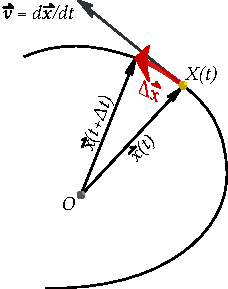
\includegraphics{01velocityistangent.pdf}
  \caption{%
  The vector function $\vx(t)$ traces out a curve in space.  The vector
  $\vx(t)$ is the position vector of a point $X(t)$ on this curve.  As we
  increase time from $t$ to $ t+\Delta t$, the point $X(t)$ moves.  The
  displacement of the point $X(t)$ is given by $\Delta\vx = \vx(t+\Delta t) -
  \vx(t)$.  The average velocity vector during this displacement is
  ``displacement/time'', i.e.\ $\Delta \vx/\Delta t$.\\
  %
  \null\qquad If we let $\Delta t\to 0$, then the average velocity becomes the
  instantaneous velocity at time $t$: $\vv = \lim_{\Delta t\to0}\Delta\vx/\Delta
  t = \vx'(t)$.  This vector is tangent to the curve traced out by the vector
  function $\vx(t)$. We call it a \emph{tangent vector}.
  }
  \label{fig:05velocity-is-deriv-of-position}
\end{figure}
\section{The derivative as velocity vector} 
\label{sec:velocity-of-vector-motion}
Suppose the motion of some point $X(t)$ in space is described by its position
vector function $\vx(t)$.  Let us try to define the instantaneous velocity of
the point.  This velocity should have magnitude (``how fast the point is
moving'') and also direction (``which way is the point going?'').  The velocity
should therefore be a vector.  To see which vector, we go back to the notion
that ``velocity'' is always ``displacement divided by time.''

We consider two instances in time, say, time $t$ and time
$t+ \Delta t$.  Then the position vectors of the point $X$ at these
two different times are $\vx(t)$ and $\vx(t+\Delta t)$.  The
displacement of the point $X$ between these two times is then
\[
\Delta \vx = \vx(t+\Delta t) - \vx(t)
\]
(see Figure~\ref{fig:05velocity-is-deriv-of-position}.)  We say that
the average velocity over the time interval from $t$ to $t+\Delta t$
is ``the displacement divided by $\Delta t$,'' i.e.
\[
\vv_{\rm average} = \frac{\vx(t+\Delta t) - \vx(t)}{\Delta t}.
\]
Note that the average velocity is a vector.  If we write it out in
components, we get a much larger formula:
\[
\vv_{\rm average} = \vek
\dfrac{x(t+\Delta t) - x(t)}{\Delta t} \\[2ex]
\dfrac{y(t+\Delta t) - y(t)}{\Delta t} \\[2ex]
\dfrac{z(t+\Delta t) - z(t)}{\Delta t} \tor.
\]
One big advantage of using vector notation is that many formulas simplify
considerably when written in terms of vectors.

To get the instantaneous velocity, we do the same thing as in one
variable calculus: we take the limit as $\Delta t\to0$ of the average
velocity over the time interval from $t$ to $t+\Delta t$.  Thus we get
\begin{equation}
  \vv(t) = \lim_{\Delta t\to0} \frac{\vx(t+\Delta t) - \vx(t)}{\Delta t}
  \stackrel{\rm def}=
  \frac{d\vx}{dt}.
  \label{eq:velocity-of-vector-motion}
\end{equation}
In terms of components this derivative is
\[
\vx'(t)= \frac{d\vx}{dt} = \vek x'(t) \\ y'(t) \\ z'(t) \tor.
\]
Thus the velocity vector of any given vector function $\vx(t)$ is the same as
the derivative of this vector function.

\section{Acceleration} 
Having found the velocity vector of a point $X(t)$ whose position vector is a
given vector function $\tpv O{X(t)} = \vx(t)$, we can also define the
\emph{acceleration vector} of the moving point.  By definition, the acceleration
vector is the derivative of the velocity vector, i.e.
\begin{equation}
	\va(t)
	= \frac{d\vv}{dt}
	= \frac{d^2\vx} {dt^2} = \vek x''(t)\\ y''(t) \\ z''(t) \tor.
	\label{eq:acceleration-vector-def}
\end{equation}
This definition is entirely analogous to the definition of acceleration
(``$a=\frac{dv}{dt}$'') from first semester calculus.  The only difference is
that, here, the position, velocity, and acceleration all have directions in
addition to magnitudes:  they are vectors.

Newton's famous law relating forces and acceleration continues to hold.  If a
point $X(t)$ moves according to some vector function $\vx(t)$, then some force
must be acting on this point. This force is a vector (it has magnitude and
direction), and, according to Newton, it is given by
\begin{equation}
  \vF = m\va = m\frac{d\vv}{dt} = m \frac{d^2 \vx}{dt^2},
  \label{eq:SirIsaacs-law}
\end{equation}
where $m$ is the mass of the object at the point $X(t)$ whose motion we are
considering.  It is always assumed to be a positive number.

Note that according to this law, the absence of forces, i.e.~$\vF=\vvv0$, is the
same as $\frac{d\vv}{dt}=\vvv0$, i.e.~no force acts on the point if and only if
its velocity vector is constant.  Here ``constant'' means constant magnitude
\emph{and} constant direction.

\section{The differentiation rules} 
Just as with ordinary derivatives, the derivatives of vector functions satisfy
certain rules, such as the product rule.  The purpose of these rules is not the
same as in one variable calculus.  There we used sum, product, quotient and
chain rules to compute derivatives of given functions without having to fall
back on the definition of a derivative all the time.  For vector functions we
do not need such rules, because we can differentiate them by simply differentiating
each of their components (see the above example).   Instead, the differentiation
rules for vector functions are mostly used to gain insight and establish general
facts about vector functions, a number of which we will see shortly.  

\subsection{The sum rule} 
The analog of the sum rule (``derivative of the sum is the sum of the
derivatives'') looks exactly like the ordinary sum rule.  It says that for any
two vector functions $\va(t)$ and $\vb(t)$ one has
\[
  \frac{d}{dt}\bigl(\va(t) \pm \vb(t)\bigr) 
  =\frac{d\va(t)}{dt} \pm \frac{d\vb(t)}{dt}.
\]

\subsection{The many product rules} 
There is no quotient rule for vector functions, simply because we have no way of
dividing vectors.  On the other hand we have two ways of multiplying vectors,
and we can also multiply vectors and numbers, so there are \emph{three}
different product rules.  Fortunately they all look like the product rule from
first semester calculus.

If $\va(t)$ and $\vb(t)$ are vector functions, and if $f(t)$ is a function,
then
\begin{align*}
  \frac{d \va(t)\dpp \vb(t)}{dt}
  &= \frac{d\va(t)}{dt} \dpp\vb(t) + \va(t) \dpp \frac{d\vb(t)}{dt}\\[1ex]
  \frac{d \va(t)\cp \vb(t)}{dt}
  &= \frac{d\va(t)}{dt} \cp\vb(t) + \va(t) \cp \frac{d\vb(t)}{dt}\\[1ex]
  \frac{d\,f(t) \va(t)}{dt}
  &= \frac{df(t)}{dt} \va(t) + f(t)  \frac{d\va(t)}{dt}
\end{align*}
In spite of the fact that these rules ``look right,'' they could still be wrong,
so to be sure we would have to prove them.  The proofs are very straightforward.
Here is a short proof for the product rule involving the dot product.  To
shorten the formulas we omit the ``$(t)$'' from all functions:
\begin{align*}
  \frac{d\va\dpp\vb}{dt}
  &= \frac{d}{dt}\bigl(a_1b_1+a_2b_2\bigr) \\
  &= \frac{da_1b_1}{dt} + \frac{d a_2b_2}{dt} \\
  &= \frac{da_1}{dt}b_1 + {\color{blue}a_1 \frac{db_1}{dt} }
  +{\color{red}\frac{da_2}{dt}b_2} + a_2 \frac{db_2}{dt}
  &\text{\footnotesize\sffamily ordinary product rule}\\
  &= \frac{da_1}{dt}b_1 + {\color{red}\frac{da_2}{dt}b_2}
    + {\color{blue}a_1 \frac{db_1}{dt} } + a_2 \frac{db_2}{dt} 
  &\text{\footnotesize\sffamily switch terms around}\\
  &= \frac{d\va}{dt}\dpp\vb + \va\dpp \frac{d\vb}{dt}.
  &\text{\footnotesize\sffamily recognize the dot-products}\\
\end{align*}


\section{Vector functions of constant length} 
\label{sec:vector-functions-of-constant-length}
As an immediate application of the product rule for the dot-product we prove the
following fact about vector functions whose length does not change, i.e.~vector
functions $\va(t)$ that change their direction, but not their length.

\null\hfill
\begin{minipage}[b]{0.4\textwidth}
\input ../figures/234/01constant-length-vector-function.pdf_tex
\end{minipage}\hfill
\begin{minipage}[b]{0.4\textwidth}\sffamily\color{darkbluegreen}
  \rule{\textwidth}{1pt}

  If a vector function $\va(t)$ has constant length, then, when the parameter $t$
  undergoes a small change $\Delta t$, the corresponding small change $\Delta \va$
  in the vector function will be almost perpendicular to $\va(t)$ itself.

  \rule[1ex]{\textwidth}{1pt}
\end{minipage}
\hfill\,
\medskip


\subsubsection*{Theorem}\itshape Let $\va(t)$ be a vector function.  Then a
necessary and sufficient condition for the length $\|\va(t)\|$ to be constant is
that $\va(t)$ and $\va'(t)$ be perpendicular for all $t$.\upshape

\begin{proof}
Differentiating both sides of the equation
\[
  \|\va(t)\|^2 = \va(t) \dpp \va(t)
\]
we get
\begin{equation}
  \frac{d}{dt}\|\va(t)\|^2 =
  \va'(t) \dpp \va(t) + \va(t) \dpp \va'(t)
  =2\va(t) \dpp \va'(t).
  \label{eq:derivative-of-squared-length}
\end{equation}
If $\va(t)$ has constant length, then $\|\va(t)\|^2$ is also constant, and thus
$\tfrac d{dt} \|\va(t)\|^2 = 0$.   Therefore, for a vector function $\va(t)$
whose length is constant, $\va(t)\dpp\va'(t)=0$, i.e.~$\va(t)\perp\va'(t)$.

Conversely, if $\va(t)$ is a vector function for which $\va(t)\perp\va'(t)$
holds for all $t$, then $\va(t)\dpp\va'(t)=0$, and
\eqref{eq:derivative-of-squared-length} implies that $\tfrac d{dt} \|\va(t)\|^2
= 0$, i.e.~that $\|\va(t)\|^2$ and hence $\|\va(t)\|$ are constant.  

\end{proof}

\section{Two examples} 
\subsection{Motion on a straight line} 
We return to the motion given by \eqref{eq:straight-line-constant-velocity},
i.e.
\begin{equation}
  \vx(t) = \va + t\vv.
\end{equation}
The velocity and acceleration are easy to compute:
\[
 \frac{d\vx(t)} {dt} = \vv, \qquad
 \frac{d^2\vx(t)} {dt} = \frac{d\vv} {dt} = \vvv0,
\]
since $\vv$ is a constant vector in this case.  

We see that if a point $X(t)$ moves according to the parametrization
\eqref{eq:straight-line-constant-velocity}, then its velocity is
constant, and its acceleration is zero.  According to Newton's law, no
force is exerted on an object undergoing this motion.

\subsection{Circular motion} 
For the point $X(t)$ moving on a circle of radius $R$ with angular velocity
$\omega$ we have \eqref{eq:constant-angluar-velocity-on-circle}, i.e.
\[
  \vx(t) = R\cos\omega t \ves1 + R\sin\omega t \ves2
\]
so that the velocity and acceleration are easy to compute:
\begin{center}
  \begin{tabular}{r@{}r@{}c@{}r}
    $\vv(t) =\vx'(t) =$\;   %%%%%%%%%%%%%%%%%%%%%%%%%%%% row 1
    &$-\omega R\sin \omega t\;\ves1$
    & $+$\;&$\omega R\cos \omega t\;\ves2$,\\
    $\va(t) =\vv'(t) =$\;   %%%%%%%%%%%%%%%%%%%%%%%%%%%% row 2
    &$-\omega^2R\cos\omega t\;\ves1$
    & $-$\;&$\omega^2R\sin \omega t\;\ves2$. 
  \end{tabular}
\end{center}

Note that the velocity vector $\vv(t)$ is perpendicular to the position
vector $\vx(t)$, as predicted in
\S~\ref{sec:vector-functions-of-constant-length}.
Our expression for the velocity vector $\vv(t)$ contains the familiar relation
between angular velocity and velocity:  the velocity $v=\|\vv(t)\|$ with which
the point $X(t)$ is moving is 
\begin{align}
  \label{eq:speed-of-circular-motion}
  v(t) &= \left\|-\omega R\sin \omega t\;\ves1
    +\;\omega R\cos \omega t\;\ves2\right\|  \\
    &= \sqrt{\omega^2R^2\sin^2\omega t + \omega^2R^2\cos^2\omega t}\notag \\
    &= \omega R.\notag
\end{align}
Hence the angular velocity of an object undergoing circular motion is
\begin{equation}
  \omega = \frac{v}{R}.
  \label{eq:angular-from-regular-velocity}
\end{equation}
\begin{figure}[h]
  \input ../figures/222/06circle3.pdf_tex
  \caption{If an object moves along a circle with constant angular velocity,
  then the force $\vF$ required to make the object follow that motion is $\vF =
  -\omega^2 \vx$.  In particular it is parallel to the position vector $\vx$
  but in the opposite direction. }
  \label{fig:circular-motion-the-force}
\end{figure}


We also note that the acceleration is a multiple of the position vector:
\[
  \va(t) = -\omega^2 \vx(t).
\]
According to Newton the force acting on the object at $X(t)$ is $\vF = m\va =
-m\omega^2\vx$, and its magnitude is
\begin{equation}
  F = \|\vF\| = \|m\omega^2\vx(t)\| = m\omega^2R,
  \label{eq:centrifugal-force}
\end{equation}
because $\|\vx(t)\|=R$ at all times.

Using \eqref{eq:angular-from-regular-velocity} we can replace the angular velocity
$\omega$ by the actual velocity, which leads to the classical formula for the
centrifugal force
\begin{equation}
  F = \frac{mv^2}{R}.
  \label{eq:centrifugal-force-from-velocity}
\end{equation}

\section{Arc length} 
\label{sec:arc-length}
For any given vector function there is a simple formula for the length of the curve
it traces out.  The formula is essentially the same as the formula for the length of
a parametric curve (or, to a lesser extent, of the graph of a function) that was
described in Math 221.  Here we repeat the intuitive derivation of the formula,
written in terms of vectors this time.

Let $\vx(t)$ ($a\le t\le b$) be a vector function.  To determine the length of the
arc traced out by $X(t)$ as $t$ varies from $t=a$ to $b$, we divide the interval
$a\le t\le b$ into many very short subintervals.  The corresponding points $X(t)$ on
the curve split the curve into many short segments, each of which will be ``close to
a line segment.''  We approximate the length of the curve by adding the lengths of
all these short segments.  Finally we take the limit in which the number of partition
points becomes infinite and our sum of lengths of short segments becomes an integral.
To see which integral we get, we need to find an expression for the length of a short
segment between two adjacent partition points on the curve.

Suppose we have two points on the curve, with parameter values $t$ and $t+\Delta t$,
respectively.  The points are $X(t)$ and $X(t+\Delta t)$, and the distance between
them is the length of the vector $\Delta\vx$ from one point to the next.
\marginpar{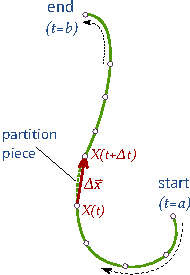
\includegraphics{01length-of-curve.pdf}}%
This vector is
\[
\Delta x = \vx(t+\Delta t) - \vx(t) =\frac{ \vx(t+\Delta t) - \vx(t)}{\Delta t} \;
\Delta t \approx \vx'(t) \Delta t,
\]
so that its length is $\approx \|\vx'(t)\| \, \Delta t$.  Adding the lengths of the
short segments together, we find that the length is approximately $\sum \|\vx'(t)\|
\, \Delta t$ (where the summation is over all short pieces of the curve).  Taking the
limit we arrive at this formula for the length of the curve traced out by $\vx(t),
a\le t\le b$:
\begin{equation}
  \text{Length} = \int_{t=a}^b \|\vx'(t)\|\; dt.
  \label{eq:length-of-curve-vector-version}
\end{equation}

This integral looks simple, but that appearance turns out to be deceptive as we find
out when we write it in terms of the components of the vector function $\vx(t)$.
Suppose $\vx(t) = x(t)\ves1 + y(t)\ves2 + z(t)\ves3$.  Then
\[
\vx'(t) = x'(t)\ves1 + y'(t)\ves2 + z'(t)\ves3,
\]
so that
\[
\|\vx'(t)\| = \sqrt{x'(t)^2 + y'(t)^2 +z'(t)^2}.
\]
Therefore the length formula \eqref{eq:length-of-curve-vector-version} of the curve
is equivalent to
\begin{equation}
  \label{eq:length-of-curve-in-components}
  \text{Length} = \int_{t=a}^b \sqrt{x'(t)^2 + y'(t)^2 +z'(t)^2}\; dt.
\end{equation}
The square root makes this formula a reliable source of very difficult integrals.  In
fact the list of curves whose length one can actually compute by doing the integral
is rather short (see Problem ...).

\section{Arc length derivative} 
Let $\vx(t)$ be some vector function that describes the motion through space of some
point $X(t)$, and let $f(t)$ be some other function.  In what follows it will help to
think of the parameter $t$ as ``time.''  Typical examples of functions $f$ that we
might want to consider are $f(t) = \|\vx(t)\|$ (the distance to the origin of the
point $X(t)$) or $f(t) = \|\vx'(t)\|$ (the speed at which the point is moving.)

To describe the rate with which $f(t)$ is changing we could compute its derivative,
\[
  \frac{df}{dt}
\]
which tells us what the ratio between the change $\Delta f$ of $f$, and the change
$\Delta t$ in the parameter $t$ is (at least approximately, if $\Delta t$ is small).
If we interpret $t$ as ``time'' then this derivative tells us how fast $f(t)$ changes
per second.  But sometimes it is more useful to know how much $f$ changes after we
have travelled a small \textit{distance} along the curve, rather than after a short
amount of time has passed.  In other words, for two nearby points $X(t)$ and
$X(t+\Delta t)$ on the curve we would like to know the ratio
\begin{equation}
  \frac{\text{change in $f$}}{\text{distance travelled}}=
  \frac{f(t+\Delta t) - f(t)}{\text{distance from $X(t)$ to $X(t+\Delta t)$}}
  \label{eq:ratio-Df-Ds}
\end{equation}
We can work this out by observing that the distance from $X(t)$ to $X(t+\Delta t)$ is
the length of the vector from  $X(t)$ to $X(t+\Delta t)$, i.e.
\[
{\text{distance from $X(t)$ to $X(t+\Delta t)$}}
=
\left\|\vx(t+\Delta t) - \vx(t)\right\|.
\]
Assuming $\Delta t$ is small, we have
\[
\left\|\vx(t+\Delta t) - \vx(t)\right\|
=
\left\|\frac{\vx(t+\Delta t) - \vx(t)}{\Delta t}\right\|\; \Delta t
\approx
\left\|\vx'(t)\right\|\; \Delta t.
\]
We substitute this in \eqref{eq:ratio-Df-Ds}, and get
\[
  \frac{\text{change in $f$}}{\text{distance travelled}}
  \approx
  \frac{f(t+\Delta t) - f(t)}{\|\vx'(t)\| \Delta t}.
\]
Now let $\Delta t\to0$:  the quantity on the left becomes what is called the
\emph{arc length derivative} of the function $f$ along the curve
$vx(t)$, and which is commonly denoted by $\frac{df}{ds}$
In the quantity on the right we recognize the derivative of $f$ with respect
to $t$ (time), which leads to
\begin{equation}
  \frac{df}{ds} = \frac{1}{\|\vx'(t)\|}\, \frac{df}{dt}.
  \label{eq:arclength-derivative-vs-time-derivative}
\end{equation}
Here $\frac{df}{dt} = f'(t)$ is the usual derivative of $f$ with respect to $t$.

If we want to emphasize the distinction between these two derivatives, then we can
call $\frac{df}{dt}$ the ``time derivative of $f$.''

\section{Unit Tangent and Curvature} 
\subsection{Unit tangent} 
We have seen that we can find a tangent vector to the curve traced out by some vector
function $\vx(t)$, simply by differentiating the vector function:  $\vx'(t)$ always
provides a tangent vector (if $\vx'(t)\ne \vvv0$).  
\marginpar{\sffamily\footnotesize%
\color{darkbluegreen}A vector with length 1 is called a \emph{unit vector}}%
In fact any multiple $\lambda\vx'(t)$ of this vector will also be a tangent
vector (provided $\lambda\ne0$.)  We can single out one special tangent vector,
by choosing $\lambda>0$ so that $\lambda\vx'(t)$ has length 1.  Since for
$\lambda>0$ we have $\|\lambda \vx'(t)\| = \lambda \|\vx'(t)\|$ the value of
$\lambda$ that will make $\lambda\vx'(t)$ a unit vector is $\lambda =
1/\|\vx'(t)\|$.

For this reason the vector
\begin{equation}
  \vT(t) = \frac{d\vx}{ds} = \frac{\vx'(t)}{\|\vx'(t)\|}
  \label{eq:unit-tangent-def}
\end{equation}
is called the \emph{unit tangent vector} to the curve corresponding to the vector
function $\vx(t)$.

\subsection{Example}  For our constant velocity parametrization 
\eqref{eq:straight-line-constant-velocity} of a straight line from
\S~\ref{sec:straight-line-constant-velocity} we have
\[
  \vx(t) = \va+t\vv,
\]
so that $\vx'(t) = \vv$ and hence
\[
  \vT = \frac{\vv}{\|\vv\|}.
\]
We see that the unit tangent vector is constant.

\subsection{Curvature and normal} 
If the curve described by a vector function $\vx(t)$ is not a straight line,
then the tangent to the curve will turn as one moves along the curve.  The
\emph{curvature vector} $\vvv\kappa$ measures how much the curve is curved.  It
is defined to be the rate of change of the unit tangent, but with respect to arc
length instead of with respect to the given parameter $t$.  Thus
\begin{equation}
  \vvv\kappa \stackrel{\rm def}= \frac{d\vT}{ds}.
  \label{eq:curvature-vector-def}
\end{equation}
According to our definition of ``derivative with respect to arc length'' the
right hand side stands for
\begin{equation}
  \frac{d\vT}{ds} = \frac{1}{\|\vx'(t)\|} \frac{d\vT}{dt}.
  \label{eq:curvature-vector-def2}
\end{equation}
To write this completely in terms of the original vector function $\vx(t)$ we
use \eqref{eq:unit-tangent-def}
\begin{equation}
  \vvv\kappa
  = \frac{1}{\|\vx'(t)\|}
  \frac{d}{dt} \Bigl\{\frac{1}{\|\vx'(t)\|}\frac{d\vx}{dt} \Bigr\}
  \label{eq:curvature-vector-in-hideous-form}
\end{equation}
This formula is not as short as the original definition
\eqref{eq:curvature-vector-def}, but it does show that the curvature vector
comes about by differentiating the vector function $\vx(t)$ twice (and dividing
by $\|\vx'(t)\|$ at the right moments.)
\bigskip

\subsubsection*{Theorem}\itshape%
The curvature vector $\vvv\kappa$ is perpendicular to the tangent,
i.e.~$\vvv\kappa\perp\vT$.\upshape

\begin{proof}
We have to show that $\vvv\kappa\dpp\vT=0$.  From the second form
\eqref{eq:curvature-vector-def2} of the definition of $\vvv\kappa$ we see
\[
  \vvv\kappa\dpp\vT = 
  \Bigl(\frac{1}{\|\vx'(t)\|} \frac{d\vT}{dt}\Bigr) \dpp \vT
  =
  \frac{1}{\|\vx'(t)\|} \;  \frac{d\vT}{dt} \dpp \vT \;.
\]
Remember that $\vT(t)$ is always a unit vector, i.e.~$\vT(t)$ has constant
length: by \S~\ref{sec:vector-functions-of-constant-length} this implies that
$\frac{d\vT}{dt}\perp\vT(t)$ and thus $\frac{d\vT}{dt}\dpp\vT=0$, so we are done.
\end{proof}

There are two concepts that are derived from the curvature vector:  the
\emph{curvature} $\kappa$ is by definition the length of the curvature vector
$\vvv\kappa$,
\begin{equation}
  \kappa = \|\vvv\kappa\| = \left\| \frac{d\vT}{ds}\right\|,
  \label{eq:curvature-def}
\end{equation}
and the \emph{normal vector} to the curve is 
\begin{equation}
  \vN = \frac{\vvv\kappa}{\|\vvv\kappa\|} 
  = \frac{\frac{d\vT}{ds}}{\left\|\frac{d\vT}{ds}\right\|}.
  \label{eq:normal-vector-def}
\end{equation}
The normal vector is undefined when $\vvv\kappa=\vvv0$, because it would require
division by zero.

Since $\vvv\kappa$ is perpendicular to $\vT$, the normal vector $\vN$ is also
perpendicular to $\vT$ (hence its name).
\begin{equation}
  \frac{d\vT}{ds} = \kappa\; \vN
  \label{eq:first-Serret-Frenet}
\end{equation}

%%\begin{equation}
%%  \frac{d\vN}{ds} = -\kappa\vT + \tau\; \vB
%%  \label{eq:second-Serret-Frenet}
%%\end{equation}
%%where
%%\[
%%\vB= \vT\cp\vN.
%%\]
%%\begin{equation}
%%  \frac{d\vB}{ds} = -\tau\; \vN
%%  \label{eq:third-Serret-Frenet}
%%\end{equation}

\section{Osculating plane} 
At any point $X(t)$ on a space curve given by $\vx(t)$ one defines the
\emph{osculating plane} to be the plane that contains the point $X(t)$ and that
is parallel to both the tangent $\vT(t)$ and normal $\vN(t)$ of the curve.

If we want to write a defining equation for the osculating plane as in
\S~\ref{sec:defining-eq-planes} then we need a vector perpendicular to the
osculating plane.  Since this plane is defined to be parallel to both $\vT$ and
$\vN$, we can find a normal vector to the osculating plane by taking the cross
product of $\vT$ and $\vN$.  This vector is called the \emph{binormal} to the
curve.  In a formula, it is defined to be
\begin{equation}
  \vB = \vT\cp\vN .
  \label{eq:binormal}
\end{equation}



\section{Problems} 

\begin{figure}[b]
  \begin{center}
    \input ../figures/234/01angularvelocity.pdf_tex
  \end{center}
\end{figure}

\begin{multicols}{2}
\problemfont
\problem Let $\ell$ be the line given by
\[
  \vx(t) = \vek 1\\ 1\\ 0\tor+ t\vek-1\\2\\1\tor.
\]
\subprob Find the unit tangent vector, the curvature, and the tangent line to the
line $\ell$ at the point where $t=2$.

\subprob Find the unit tangent vector, the curvature, and the tangent line to the
line $\ell$ at any point on the line.

\problem What sign does $\omega$ have in 
Figure~\ref{fig:circular-motion-the-force}~?  How would the figure change if we
change the sign of $\omega$?  Does the force $\vF$ on the object change if we
change the sign of $\omega$?

%% \problem While reading the definition of the curvature vector and especially after
%% seeing the not-so-nice formula \eqref{eq:curvature-vector-in-hideous-form} for the
%% curvature vector it is natural to think ``isn't there a simpler way to define
%% curvature?''  Here is one attempt.  The questions invite you to judge this
%% alternative definition of ``curvature'' on its merits.
%% 
%% For any parametric curve a tangent vector is given by $\vx'(t)$.  To see if the
%% curve deviates from being a straight line we simply check if $\vx'(t)$ changes,
%% and we can do this by computing the derivative of $\vx'(t)$.  So let us define
%% \[
%%   \vK(t) = \vx''(t),
%% \]
%% and let us see if this measures how much the curve is curved.  (As
%% mathematicians we can define whatever we want, and this definition is a lot
%% simpler than \eqref{eq:curvature-vector-in-hideous-form}.)
%% 
%% \subprob True or False:  \textit{if $\vK(t)=\vvv0$ for all $t$ then the curve is
%% a straight line} \dots ?
%% 
%% \subprob Compute $\vK(t)$ for $\vx(t) = \tvek t^2\\t^2\ttor$, and draw the curve
%% traced out by this particular vector function.
%% 
%% \subprob True or False: \textit{if $\vx(t)$ traces out a straight line then
%% $\vK=\vvv0$} \dots ?
%% 
%% \subprob Conclusion: To what extent does the statement ``$\vK=\vvv0$'' have
%% anything to do with the statement ``$\vx(t)$ traces out a straight line''?

\problem Suppose a point $P$ is rotating around a line $\ell$, keeping 
its distance to the line fixed at $r$, and moving in a plane perpendicular to
the line.  Suppose the point has angular velocity $\omega$: this means that
during a time interval of length $t$ the angle swept out by the line segment
connecting $P$ to $\ell$ is exactly $\omega t$.

In a previous math or physics class it was shown that the velocity of
the point $P$ is $\omega r$, where $r$ is the distance from $P$ to
the line $\ell$.

The \emph{angular velocity vector} is defined to be the vector
$\vvv\omega$ whose length is $\omega$, and that is parallel to the
line $\ell$.  There are two such vectors ($\pm \vvv\omega$).  By
definition $\vvv\omega$ points in the direction in which a screw
would move if it were turning in the same direction as the point $P$.

\subprob Assuming the line $\ell$ passes through the origin show from the 
drawing that the velocity vector of the point $P$ is $\vv$ is given by $\vvv\omega
\cp \vx$.  You can do this in two steps, namely:

%% \setlength{\itemindent}{0pt}
%% \setlength{\listparindent}{0pt}
%% \setlength{\labelwidth}{0pt}
\begin{list}{---}
  {\setlength{\leftmargin}{0pt}}
\item \itshape show that $\vvv\omega\cp\vx$ has the same direction as $\vv$,
\item \itshape show that $\vvv\omega\cp\vx$ has the same length as $\vv$.
\end{list}

\subprob Show that the acceleration vector is given by $\va =
\vvv\omega\cp(\vvv\omega\cp\vx)$.  (hint: don't use the drawing, but combine
the definitions of $\vv$ and $\va$, in 
\eqref{eq:velocity-of-vector-motion} and \eqref{eq:acceleration-vector-def}
and also the product rule; finally, keep in mind that you have just found that
$\vv=\vvv\omega\cp\vx$.)

\subprob If someone told you they had computed the acceleration vector
and found
\[
  \va =(\vvv\omega\cp\vvv\omega)\cp\vx,
\]
could they be right?
Explain!  What if they told you they got $\va =
\vvv\omega\cp\vvv\omega\cp\vx$?

\subprob True or False (explain your answers):

(a) $\vv\perp \vx$?\qquad (b) $\va\perp \vv$? \qquad (c) $\va$ and
$\vx$ are parallel?

\subprob Include the acceleration vector $\va$ in the above drawing.

\problem Consider the ``twisted cubic,'' 
i.e.~the curve given by $\vx(t) = t\ves1+t^2\ves2+t^3\ves3$.

\subprob Find a parametrization for the tangent to the curve at the point where
$t=1$.  Where does this point intersect the $xy$-plane?

\subprob For any given $t$ find the tangent line to the curve 
at the point $X(t)$, and find where this curve intersects the $xy$-plane.  

\problem Compute the length of one full turn of the helix by taking the
parametrization given in \eqref{eq:helix-def} and computing the length of the
segment with $0\le \theta\le2\pi$.

After computing the length, consider this:  let $P$ be the perimeter of the
circle underneath the helix, and let $H$ be the height achieved by one full turn
of the helix.  Show that the length $L$ of the helix satisfies $L^2 = P^2+H^2$.


\problem There is a multistory parking ramp where the way out 
is a path in the shape of a helix that is wound around the outside of the
building.  As a car drives down this path at night its headlights shine a spot
on the ground.  Which curve is traced out by this light spot as the car drives
all the way down?

Make a good drawing.  Assume for simplicity that the center of the Parking ramp
is the $z$-axis.

\problem Compute the tangent, curvature, normal and binormal 
for the following curves

\subprob The parabola: $\vx(t) = \tvek t^2 \\ t\ttor$.  At which point  
on the curve is the curvature the largest?  

\subprob Neil's parabola: $\vx(t) = \tvek t^2\\ t^3\ttor$.  At which point on  
the curve is the curvature the largest?

\subprob The helix: $\vx(\theta) =\tvek R\cos \theta \\ R\sin \theta\\  
a\theta\ttor$ (see \S~\ref{sec:helix} for an explanation of the constants $R$ and
$a$).  At which point on the curve is the curvature the largest?

\subprob The graph of $y=e^x$  
by using the parametrization $\vx(t) = \tvek t \\e^{t}\ttor$.
Where on the graph is the curvature the largest?
\answer $\kappa(x) = \dfrac{e^x}
{\bigl(1+e^{2x}\bigr)^{3/2}}$.

To find the point with largest curvature: 
$\kappa'(t) = \dfrac{e^t} {\bigl(1+e^{2t}\bigr)^{5/2}}
\bigl(1-2e^{2t}\bigr)$, so the maximal curvature (smallest radius of
curvature) occurs when $x=-\frac{1} {2}\ln{2}$.
\endanswer

\problem
\subprob
A vector function $\vx(t)$ describes the motion of a point in space.  It is known that there is a constant vector $\vm$ such that the velocity $\vv(t)$ always satisfies $\vv(t) = \vm \times \vx(t)$.  Show that the quantity $\vm\cdot \vx(t)$ is constant.
\answer
To show that $\vm\dpp\vx(t)$ is constant we differentiate it with respect to time:
\[
\frac{d \vm\dpp\vx(t)} {dt} = \vm\dpp\vx'(t) = \vm\dpp\bigl(\vm\cp\vx(t)\bigr) = 0,
\]
because the cross product $\vm\cp\vx(t)$ is always perpendicular to the vector $\vm$.
\endanswer
\subprob 
A vector function $\vx(t)$ describes the motion of a point in space.  It is known that there is a constant vector $\vm$ such that the velocity $\vv(t)$ and acceleration $\va(t)$ always satisfy $\va(t) = \vm \cp \vv(t)$.

Show that the quantity $\|\vv(t)\|^2$ is constant.

Then show that the angle between $\vm$ and $\vv(t)$ is constant (hint: look at the dot product $\vm\dpp\vv(t)$).

\subprob
A vector function $\vx(t)$ describes the motion of a point in space.  It is known that there is a constant number $C$ such that the acceleration $\va(t)$ always satisfies $\va(t) = -C \vx(t)$.  Show that the quantity $\vx(t)\cp\vv(t)$ is constant (where $\vv(t)$ is by definition the velocity vector).

%% \problem Show: a curve is plane if and only if its torsion vanishes 
%%($\tau = 0$).
%%
%%\problem Express $\vx'\cp\vx''$ in terms of $\kappa, \tau, \vT, \vN,
%%\vB$ and $\|\vx'\|$.
%%
%%\problem Let $A(h)$ be the area of the triangle with vertices 
%%$\vx(t-h)$, $\vx(t)$ and $\vx(t+h)$.  Compute $\DS \lim_{h\to 0}
%%\frac{A(h)}{h^3}$.  Hint: use a Taylor expansion $\vx(t+h) = \vx(t) +
%%h\vx'(t) + \frac{h^2}{2}\vx''(t) + o(h^2)$.

\noproblemfont
\end{multicols}


% Time-stamp: Sun Jul 28 14:00:00 2013
% !TEX root =  free234.tex
\chapter{Functions of more than one variable} 

\section{Functions of two variables and their graphs} 
\subsection{Definition} 
A function of two variables has two ingredients: a \textit{domain} and \textit{a
rule}.  The domain of the function is a collection of points in the $xy$-plane.
For each point $(x,y)$ from the domain of the function, the rule
should tell us how to find the function value $f(x,y)$.

Just as with functions of one variable, the ``rule'' that gives us the function
value is often specified by some formula, e.g.~$f(x,y) = x+y$.  The domain of a
function is the set of points at which we define the function.  This can in
principle be any set of points in the plane.  Typically the domain will be a
rectangle, or a disc, or it could be the entire $xy$-plane, possibly with some
points and lines removed.

\begin{figure}[h]
  \begin{center}
    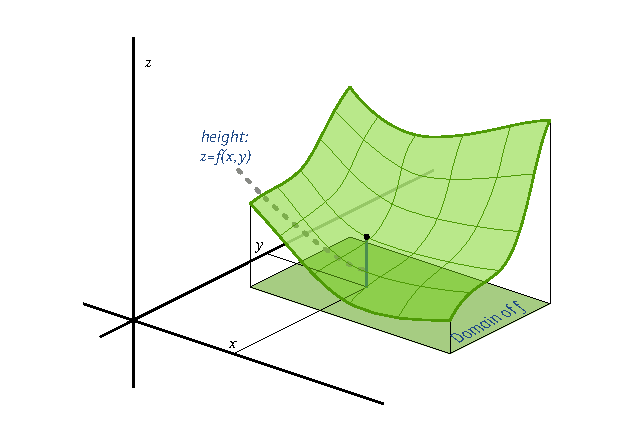
\includegraphics{01Agraph.pdf}
  \end{center}
  \caption{The graph of some function, and its domain (a rectangle in this
  example).}
  \label{fig:01Agraph}
\end{figure}

\subsection{Graphs} By definition, the graph of a function 
$z=f(x,y)$ is the collection of all points $(x,y,z)$ in three dimensional space
that satisfy the equation $z=f(x,y)$.

The graph is usually a surface that floats above (or below) the domain of the
function (see Figure~\ref{fig:01Agraph}).

\subsection{Level sets}  The graph of a function of two variables 
is a surface sitting in three dimensional space, which can be difficult to draw
or visualize.  Instead of looking at the graph we can also consider its level
sets.  If $c$ is any real number, then, by definition, the \emph{level set at
level $c$} of the function is the set of all points $(x,y)$ in the plane that
satisfy $f(x,y) = c$.

\begin{figure}[h]
  \begin{center}
    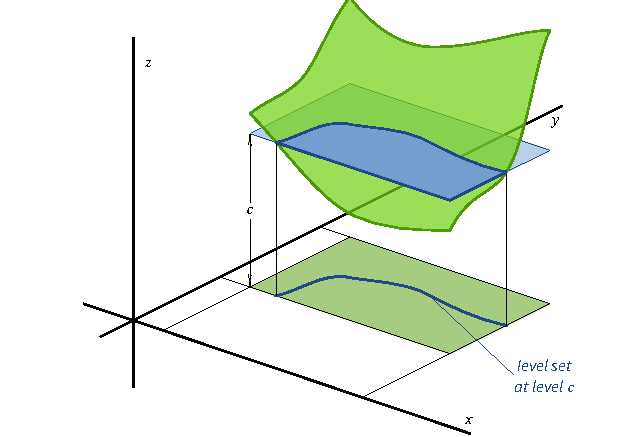
\includegraphics{01Agraphwithlevelsets.pdf}

    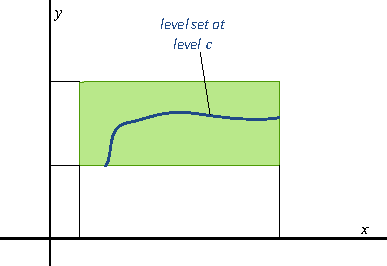
\includegraphics{01levelsets-without-the-graph.pdf}
  \end{center}
  \caption{The graph of some function (\textit{top}), and a construction of one
  of its level sets (\textit{bottom}).  Note that \textit{by definition} the
  level set (``at level $c$'') is the curve in the $xy$-plane under the graph:
  it is obtained by intersecting the graph of the function with a horizontal
  plane at height $c$, and then projecting this curve of intersection onto the
  $xy$-plane.  }
  \label{fig:01Agraph}
\end{figure}

Since the level set is the set of all solutions to the equation $f(x,y)=c$, one
often uses the notation $f^{-1}(c)$ (``$f$-inverse of $c$'') for the level set.
We can summarize the definition in an equation:
\[
  f^{-1}(c)
  =
  \bigl\{ (x,y) : f(x,y) = c\bigr\}.
\]%
\marginwarning%
Note that the definition says that $f^{-1}(c)$ \emph{is not a number, but a set
of points!}

Level sets tend to be curves in the $xy$-plane, although in general level sets
can have any shape (see Problem~\ref{prb:distance-to-square-level-sets} for an
example.)  They are usually easier to draw than the graphs of the corresponding
functions.

\subsection{An example from the ``real'' world} 
\label{sec:01mendotaexample}  Here is a function of local interest.  The domain
of the function is the water surface of Lake Mendota (let's pretend this is a
plane domain), and the function, which we will call $d$ instead of $f$, is given
by $d(x, y) = $ the depth of the lake at location $(x, y)$.  There is no formula
for this function, but the Wisconsin Department of Natural Resources has
measured the depth and presented the results in terms of the level sets of the
function $d$.


\begin{figure}[ht]
  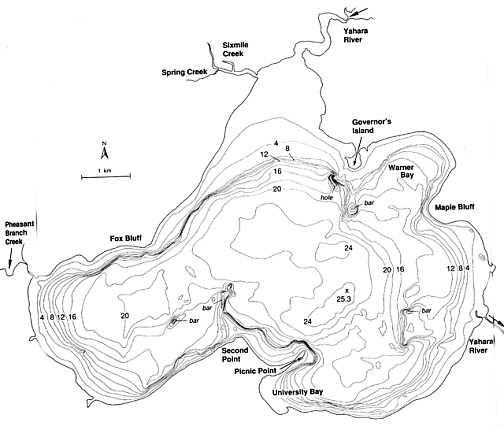
\includegraphics[width=0.70\textwidth]{01Mendota.jpeg}
  \caption{  The level curves of a function $z=d(x, y)$.  The domain of this
  function is the lake surface, and $d(x, y)$ is the depth in meters of Lake
  Mendota at $(x, y)$.  To see the graph of the function we could try to drain the
  lake.\\
  \null\quad%
  See \url{http://limnology.wisc.edu/lake_information/mendota/mendota.html} }
\end{figure}

\subsection{A comment about language and set-theoretic notation} 
We will often say ``consider a function $z=f(x,y)$\dots'', but there is a
sense in which this is incorrect.  It is convenient to say ``consider a function
$z=f(x,y)$\dots'' since it not only names the function, but it also gives the
independent variables $x$, $y$, and the dependent variable $z$ a name.
Nevertheless, the symbol in the equation $z=f(x,y)$ that actually represents the
function is ``$f$''.  The correct way of introducing the function\footnote{%
Saying ``consider the function $z=f(x,y)$\dots'' to introduce the function $f$ is
like saying ``Please meet my brother Joe, Bill, and Sue'' when you want to
introduce your brother Joe, who happens to be standing next to Bill and Sue.  To
introduce your brother, you would of course say ``Please meet my brother
Joe.'' and to introduce the function you should really say ``Consider the
function $f$.''}
would be to say ``consider a function $f$.''

In fact, in the notation that is used in modern mathematics one would write
``Consider the function $f:D\to\R$\dots''  Here $f$ is the name of the function
we are introducing, $D$ is the domain of that function (so $D$ is a set of
points in the plane), and $\R$ stands for the set of real numbers, indicating
that computing $f$ always results in a real number.

\subsection{Vector notation} If $\vx$ is the position vector 
of the point $(x, y)$ in the plane, i.e.\ if $\vx = \tvek x\\ y\ttor$, then one
sometimes writes
\[
f(x, y)  = f(\vx).
\]
Physicists have a preference for $\vr$ instead of $\vx$ (because they call the
position vector the ``radius vector''), and will write $f(x,y) = f(\vr)$.



\section{Linear functions} 
The simplest function of one variable are those of the form $f(x) = ax+b$.
Their graphs are lines, and we called them linear functions.

A linear function of two variables is a function $f$ of the form
\begin{equation}
  z=f(x,y) = ax+by+c,
  \label{eq:linear-function}
\end{equation}
where $a,b,c$ are constants.

\begin{figure}[h]
  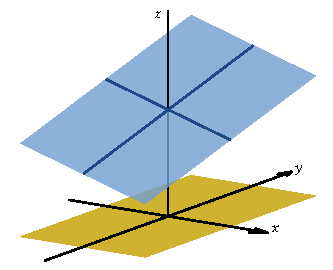
\includegraphics{01graph-of-a-linear-function.pdf}
  \caption{The graph of a linear function $z=ax+by+c$. }
  \label{fig:graph-of-lin-f}
\end{figure}
The graph of a linear function is always a plane.  Indeed, the graph consists of
all points $(x,y,z)$ that satisfy the equation
\[
  -ax-by+z = c,
\]
which we can write as 
\[
  \vn\dpp\vx = \vn\dpp\vp,
\]
where
\[
  \vn = \vek -a\\ -b\\ 1\tor, \quad \text{and}\quad
  \vp = \vek 0 \\ 0 \\ c\tor.
\]

\section{Quadratic forms} 
\label{sec:quadratic-forms}%
After learning about linear functions in pre-calculus one usually goes on to
quadratic functions.  We will do the same for functions of two variables and
study \textit{Quadratic Forms}.  Just as in the one variable case where
quadratic functions can have a maximum or minimum, quadratic forms provide
examples of functions of two variables that can have a maximum or a minimum, or,
it turns out, a third kind of ``min-max'' or ``saddle shape.'' They provide the
basic profile of what we will run into when we look for local minima and maxima
of functions of two variables.  In particular, the technique of classifying
quadratic forms by completing the square, which we will see in this section, is
the key to the second derivative test for functions of more than one variable.


\subsection{Definition} 
The general quadratic form in two variables is
\begin{equation}
  f(x,y) = Ax^2 + Bxy + Cy^2,
  \label{eq:general-quadratic-form}
\end{equation}
where $A$, $B$, and $C$ are constants.  Depending on the values of these
constants the graphs of the functions can have a number of different shapes.

In addition to these quadratic forms one can also consider the more general
class of quadratic functions,
\[
  f(x,y) = Ax^2 + Bxy + Cy^2 + Dx + Ey + F,
\]
which also have terms of degree 1 and 0.
We will restrict ourselves to quadratic forms (for now).

\subsubsection*{The prototypical examples}

There are several important special cases that are representative of what the
graphs of quadratic forms can look like.  These special cases are
\begin{subequations}
  \begin{align}
    f(x,y) & = x^2+y^2, \text{ and } g(x,y) = -x^2-y^2,
    \label{eq:qform-definite}\\
    h(x,y) & = x^2, \text{ and } \tilde h(x,y) = -x^2,
    \label{eq:qform-semidefinite}\\
    k(x,y) & = xy
    \label{eq:qform-indefinite}
  \end{align}
\end{subequations}
Their graphs are discussed in Figure~\ref{fig:typical-q-forms}.
\begin{figure}[b]\flushleft
\color{darkbluegreen}\sffamily
\noindent%
\rule{\textwidth}{1pt}
\vglue2pt
\noindent%
\begin{minipage}{0.42\textwidth}
  The two forms $f$ and $g$ from \eqref{eq:qform-definite} are called
  \emph{\color{badgerred}definite}, since they cannot change sign:
  \[
    f(x,y) = x^2+y^2
  \]
  is the sum of two squares, and therefore is always positive, unless both $x$
  and $y$ vanish.  Similarly, $g(x,y) = -f(x,y)$ is always negative, except at
  $(x,y) = (0,0)$.
\end{minipage}\hfill
\parbox{0.55\textwidth}{
  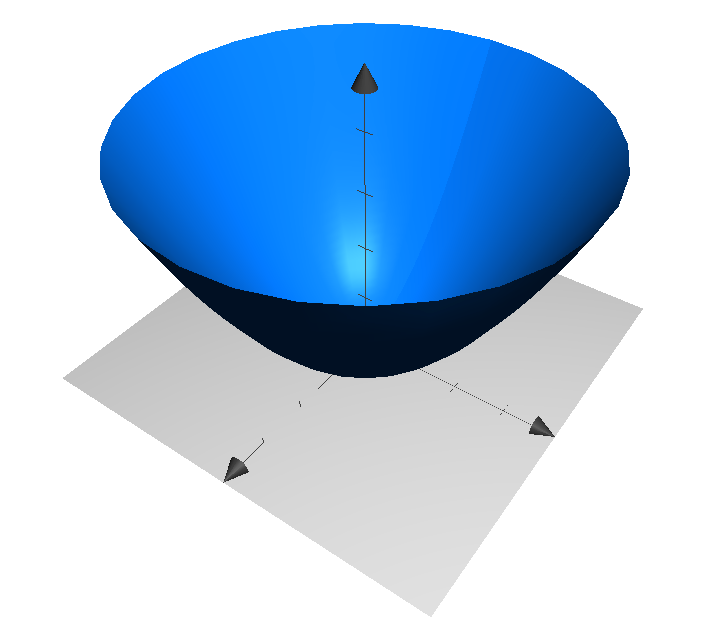
\includegraphics[width=0.25\textwidth]{01minimum.png}
  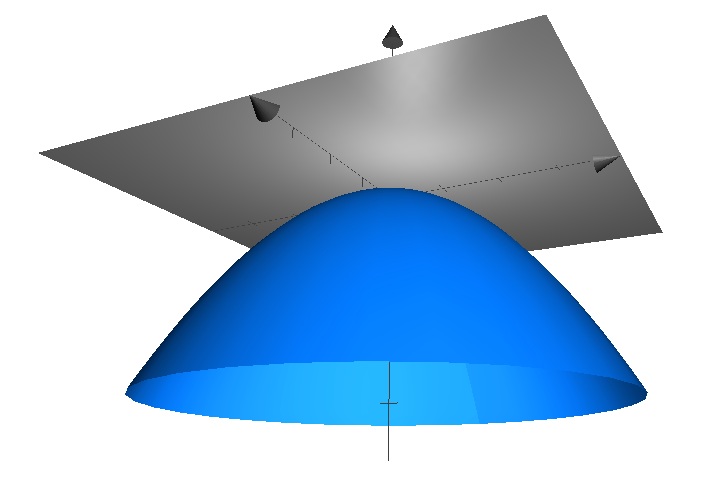
\includegraphics[width=0.25\textwidth]{01maximum.png}
  }


\noindent%
\rule[-0.5ex]{0pt}{1ex}%
\rule{\textwidth}{0.2pt}
\noindent%
\begin{minipage}{0.42\textwidth}
 The form $h(x,y) = x^2$ is called
  \emph{\color{badgerred}semidefinite} because it too cannot change its sign.
  Clearly, $h(x, y)=x^2$ is never negative, but for $h(x, y)$ to be positive, we
  need $x\neq0$.
  So, the function $h(x,y)$ is positive, except on the line $x=0$ (the $y$
  axis).  The graph of the function $\tilde h(x, y) = -y^2$ is similar, but
  upside down.
\end{minipage}
\parbox{0.55\textwidth}{
  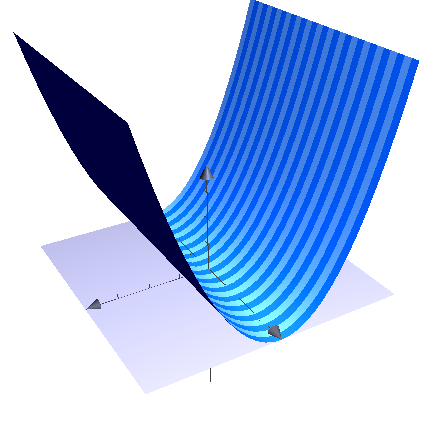
\includegraphics[width=0.25\textwidth]{01degenerate-minimum.png}
  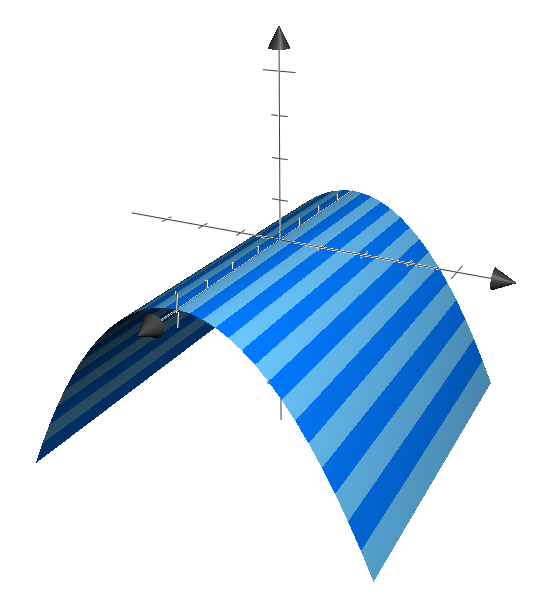
\includegraphics[width=0.25\textwidth]{01degenerate-maximum.png}
}


\noindent%
\rule[-0.5ex]{0pt}{1ex}%
\rule{\textwidth}{0.2pt}
\noindent%
\begin{minipage}{0.42\textwidth}
 The form $k(x, y) = xy$ is called \emph{\color{badgerred}{indefinite},} because
 it can be both positive and negative:  if $x$ and $y$ have the same sign, then
 $xy>0$, but if they have opposite signs, then $xy<0$.  Thus the graph of $z=xy$
 lies above the $xy$-plane in the first and third quadrants, and below the
 $xy$-plane in the second and fourth quadrants.
\end{minipage}
\parbox{0.55\textwidth}{%
\def\svgwidth{0.25\textwidth}
  \input ../figures/234/01saddle-signs.pdf_tex
  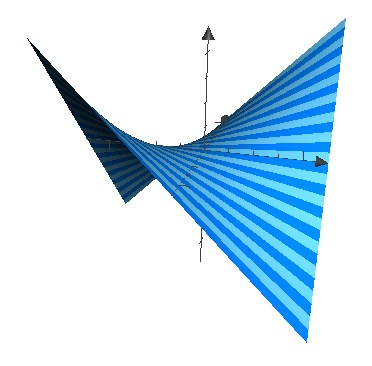
\includegraphics[width=0.25\textwidth]{01saddle-stripes.png}
  }

\noindent%
\rule{\textwidth}{1pt}
\caption{Graphs of some representative quadratic forms.}
\label{fig:typical-q-forms}
\end{figure}

\subsection{Classifying quadratic forms -- the general procedure} 
All quadratic forms have graphs that look like one of the examples shown above
-- but how can we tell which it is?  In other words, if $Q(x, y)$ is a given
quadratic form how can we tell if it is definite, indefinite, or semidefinite?
How do we know for which $(x, y)$ the form $Q(x, y)$ is positive or negative?
It turns out that we can always find out by using the trick of ``completing the
square.''

The general procedure for a given quadratic form $Q(x, y) = Ax^2+Bxy+Cy^2$ is as
follows:
\begin{enumerate}
\item If $A=0$, then we really have $Q = Bxy+Cy^2$ and we can factor $Q$ as
  \[
    Q(x, y) = (Bx+Cy)y.
  \]
\item Assume $A\ne 0$.
  We factor out $A$, and complete the square for the
  first two terms:
\begin{align*}
    Q(x, y) &= A\Bigl\{x^2+\frac{ B}{A}xy + \frac CA y^2\Bigr\}\\
    &=A \Bigl\{\bigl(x+\frac{B}{2A}y\bigr)^2 - \bigl(\frac{B}{2A}y\bigr)^2 + 
    \frac CA y^2\Bigr\}\\
    &=A \Bigl\{
    \underbrace{
      \bigl(x+\frac{B}{2A}y\bigr)^2
    }_{u^2}
    + \underbrace{
      \frac{\color{badgerred}4AC-B^2}{4A^2}y^2
    }_{\pm v^2}
    \Bigr\}.
\end{align*}
\item If $4AC-B^2>0$, then the expression in braces is positive, and we can
  write 
  \[
    Q(x, y) = A(u^2+v^2), \quad\text{where}\quad
    u = x+\frac{B}{2A}y, \text{ and }
    v = \frac{\sqrt{4AC-B^2}}{2A}y.
  \]
  Depending on the sign of $A$ our function is always positive or always
  negative, and we say the form is \emph{positive definite} or \emph{negative
  definite.}
\item If $4AC-B^2<0$, then we have
  \[
    Q(x, y) = A(u^2-v^2), \quad\text{where}\quad
    u = x+\frac{B}{2A}y, \text{ and }
    v = \frac{\sqrt{B^2-4AC}}{2A}y.
  \]
  When this happens we can factor the quadratic form, i.e.~we have
  \[
    Q(x, y) = A (u+v)(u-v).
  \]
  The form is \emph{indefinite.}
\item in the only remaining case we have $4AC-B^2=0$, so that
  \[
    Q(x, y) = A\Bigl(x+\frac{B}{2A}y\Bigr)^2.
  \]
  In this case the form is a perfect square (times $A$).
  The form is \emph{semi-definite.}

\end{enumerate}
To understand this procedure it is perhaps best to look at how it works in some
examples.

\subsection{Classifying quadratic forms -- two examples} 

\subsubsection{An indefinite quadratic form} 
\label{sec:quad-form-example-indefinite}
Consider the form $Q(x, y) = -3x^2+9xy+6y^2$. We rewrite this as
follows:
\begin{align*}
  Q&= -3x^2+6xy+9y^2\\
  &=-3\bigl(x^2 - 2xy -3y^2\bigr) \\
  &= -3\bigl[\underbrace{x^2  - 2xy + y^2}_{} -4 y^2\bigr]
  & \parbox{160pt}{\dfnt%
  complete the square}\\
  &= -3\bigl[(x-y)^2 - 4y^2\bigr]
  & \parbox{160pt}{\dfnt\raggedright%
   in this case we get the difference of two squares,
   so use $a^2-b^2 = (a-b)(a+b)$}\\
  &= -3(x-y-2y)(x-y+2y) \\
  &= -3(x-3y)(x+y).
\end{align*}
This shows that $Q(x, y) > 0$ when $y>\tfrac 13 x$ or $y<-x$,
and $Q(x, y) <0$ when $-x < y < \tfrac 13x$.

\begin{figure}[h]
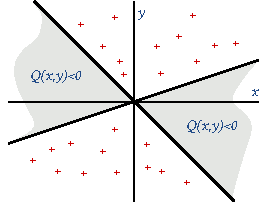
\includegraphics{03Q-signs.pdf}
\caption{The signs of the quadratic form in example
  \ref{sec:quad-form-example-indefinite}.}
\end{figure}

\subsubsection{A positive definite quadratic form}
\label{sec:quad-form-example-positive-definite}
To see a different example, consider the quadratic form $Q(x, y) = 2x^2-4xy+6y^2$.
By completing the square we can write it as
\begin{align*}
  Q(x, y)
  &= 2\, \bigl\{x^2 -2xy + 3y^2\bigr\} & \\
  &= 2\, \bigl\{\color{blue}x^2-2xy+y^2\color{black} + 2y^2\bigr\}
  &\parbox{160pt}{\dfnt the square is complete}\\
  &= 2\, \bigl\{\color{blue}(x-y)^2\color{black} + 2y^2\bigr\} &\\
  &= 2(x-y)^2 + 4y^2.
\end{align*}
We see that this particular quadratic form is positive definite.


\section{Functions in polar coordinates $r,\theta$} 
\label{sec:functions-in-PC}%
Recall that instead of using Cartesian coordinates $(x,y)$ to specify the location
points in the plane, we can also use polar coordinates.  In many cases it is much
easier to describe a function using polar coordinates than in Cartesian coordinates.

To go back and forth between Cartesian and Polar Coordinates we can use the following
relations
\begin{subequations}
  \begin{align}
    x &= r\cos\theta \\
    y &= r\sin\theta \\
    r &= \sqrt{x^2 + y^2} \\
    \text{\color{red}\carefulnow}\; \theta &= \arctan\frac{y}{x}\; 
    \text{\color{red}\carefulnow}
  \end{align}%
  \label{eq:PC-xy-relations}%
\end{subequations}%
The equation for $\theta$ is only valid for $x>0$, where $-\frac\pi2 < \theta <
\frac \pi2$.  In other regions of the plane there are other expressions relating
$\theta$ to $(x,y)$.  See problem~\ref{prb:polar-angle-formula}.

\begin{figure}[h]
  \flushleft%
  \parbox{0.45\textwidth}{
  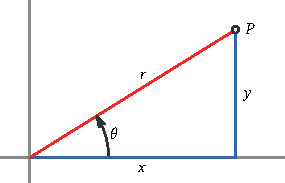
\includegraphics{01PC.pdf}
  }\hfill
  \parbox{0.45\textwidth}{
  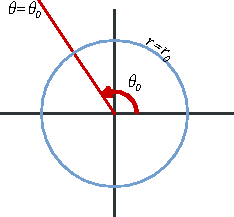
\includegraphics{01theta-r-constant.pdf}
  }
  \caption{Polar coordinates are defined in the picture on the right (see also
  equations \eqref{eq:PC-xy-relations}).  On the left:  the set of points at which
  $\theta$ has one given value $\theta_0$ form a half line emanating from the origin
  that makes an angle $ \theta_0$ with the positive $x$-axis.   The set of points at
  which $r$ has a given value $r_0$ form a circle centered at the origin, with radius
  $r_0$.}
\end{figure}

The simplest kinds of functions one can consider in polar coordinates are those that
only depend on one of those coordinates, i.e.~functions that only depend on the
radius $r$, and functions that only depend on the polar angle $\theta$.
Let's look at some examples of such functions.

\subsection{Radially symmetric functions} 
\label{sec:functions-in-PC-radial}%
The functions
\[
  f(x, y) = x^2+y^2, \quad
  g(x, y) = \sqrt{x^2+y^2}, \quad
  h(x, y) = \ln\bigl(x^2+y^2\bigr),
\]
all can be expressed in terms of the radius $r$ only.  Namely, using $r^2=x^2+y^2$, we
have
\[
  f(x, y) = r^2, \quad
  g(x, y) = r, \quad
  h(x, y) = \ln r^2 (= 2\ln r).
\]
In general, a function $z=f(x, y)$ that can be written in terms of the radius $r$
only, i.e. a function for which there is some function $\Phi$ of one variable with
\[
  f(x, y) = \Phi(r), \quad
  \text{i.e. } f(x, y) = \Phi\bigl(\sqrt{x^2+y^2}\bigr),
\]
is called a \emph{radially symmetric function.}  

Since a radially symmetric function only depends on the radius $r$, its level sets
consist of circles centered at the origin (one exception:  the origin, $r=0$ can
also be a level set, and this is obviously not a circle but a point.)

As an example, we consider the function $g(x, y) = \sqrt{x^2+y^2} = r$ in more detail.
The function $\Phi$ of one variable here is $\Phi(r) = r$.  We can try to visualize
the graph of $g$ by first looking at the positive $x$-axis only.  There we have $f(x,
0)=\sqrt{x^2} = x$.  We get the graph of $g$ by revolving the graph of $z=x$ around
the $z$-axis.  See Figure~\ref{fig:graph-of-z-is-r}.
\begin{figure}[t]
  \def\svgwidth{0.6\textwidth}%
  \input ../figures/234/01cone.pdf_tex
  \caption{\textbf{Radially symmetric functions.}  The graph of $z=r$.}
  \label{fig:graph-of-z-is-r}
\end{figure}

\subsection{Functions of $\theta$ only} 
\label{sec:functions-in-PC-theta}%
Here are two functions that happen to depend on the polar angle $\theta$ only:
\[
  f(x, y) = \sin\theta, \qquad h(x, y) = \theta.
\]
We can rewrite these functions in terms of $x$ and $y$ by using the relations between
Cartesian and Polar coordinates \eqref{eq:PC-xy-relations}.  We get
\[
  f(x, y) = \sin\theta = \frac{y}{r} = \frac{y}{\sqrt{x^2+y^2}}
\]
for $f$, and 
\[
  h(x,y) = \theta = \arctan \frac{y}{x}
\]
for $h$, at least in the right half plane where $x>0$. 

A function that only depends on $\theta$ is constant on rays emanating from the origin
because the polar angle $\theta$ is constant on such rays. The level sets of such
a function therefore consist of half-lines (``rays'') starting at the origin. Its
graph consists of ``spokes'' attached to the $z$-axis.  Each spoke lies above a ray
in the $xy$-plane with some polar angle $\theta$, and is attached to the $z$-axis at
a height given by the function value.  As we vary $\theta$, the spoke rotates around
the vertical axis and moves up or down, as dictated by the function.
Figure~\ref{fig:graph-of-f-of-theta} shows what happens for $f(x, y) = \sin\theta$.

\begin{figure}[h]
  \begin{minipage}{0.4\textwidth}
    \centering
    \dfnt 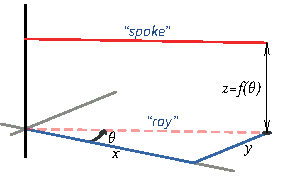
\includegraphics{01PC-graph-of-f-theta.pdf}\\
    The graph of a function of $\theta$ only consists of horizontal spokes attached to
    the $z$-axis.
  \end{minipage}
  \begin{minipage}{0.55\textwidth}
    \centering
    \dfnt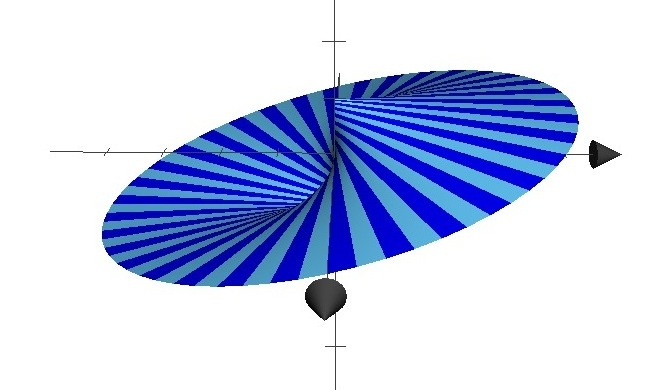
\includegraphics[width=0.95\textwidth]{01function-of-theta.jpeg}\\
    The graph of $z=\sin\theta$\\
    (the $x$-axis is coming right at us.)
  \end{minipage}
  \caption{}
  \label{fig:graph-of-f-of-theta}
\end{figure}

The function $z=\theta$ has a simpler formula in polar coordinates but actually has a
more complicated graph. Let us try to visualize its graph:  the spokes that make up
the graph are horizontal, attached to the $z$-axis, and are at height $\theta$.  If
we increase the angle $\theta$ the spokes go up at a steady rate in a way that should
remind us of a helix (see \S~\ref{sec:helix} and Figure~\ref{fig:helix}).  Based on
this description its graph should look like the surface drawn in
Figure~\ref{fig:helicoid}.  The surface is called the \emph{helicoid}, and it is
\emph{not} the graph of a function (it fails the ``vertical line test.'')  We could
have known this from the beginning , because when we described our function as $f(x,
y) = \theta$, we should have immediately asked \textit{which $\theta$?}  The polar
angle $\theta$ of any given point is only determined up to a multiple of $2\pi$.  The
``graph'' that we have drawn of the ``function'' $z=\theta$ reflects this.  To make
$h(x, y) = \theta$ into an honest function we have to say which of the many
possible angles $\theta$ we choose when we are given a point.  One possible choice is
to always require the polar angle $\theta$ to lie between $0$ and $2\pi$ (radians).
More precisely, we can insist on 
\[
  0\leq \theta < 2\pi.
\]
If we do this then there is a unique angle $\theta$ for each point $(x,y)$ in the
plane.  The graph of this function is shown on the right in
Figure~\ref{fig:helicoid}.  

\begin{figure}[h]
  \parbox{0.4\textwidth}{ \input ../figures/234/01helicoid-many.tex }
  \hfill
  \parbox{0.4\textwidth}{ \input ../figures/234/01helicoid-one.tex }
  \caption{The graph of $z=\theta$ is the helicoid.  It is not the graph of a function,
  but one can extract a function by choosing a ``branch'' of the function.  One
  possible choice, drawn here on the right, is to restrict the polar angle $\theta$ to
  the interval $0\leq \theta < 2\pi$.  There are many other possible choices.  }  
  \label{fig:helicoid}
\end{figure}

\section{Methods of visualizing the graph of a function}  

\subsection{Freezing a variable}  

If a function is not familiar, then a good strategy for drawing its graph is to
``\emph{freeze a variable.}'' In other words, to analyze a function $ z=f(x,y) $ we
pretend $y$ is a constant: then $x$ is the only independent variable, and we can try
to draw the graph of the function $z=f(x,y)$, now thinking of this as a function of
only one variable. This graph is a curve in the $xz$ plane. We get one such curve for
each choice of $y$. Piecing these graphs together then gives us the graph of the
two-variable function $z=f(x,y)$.

We could apply the same procedure with the roles of $x$ and $y$ switched: i.e.  for
each fixed $x$ you try to graph $z=f(x,y)$ as a function of the variable $y$ only,
after which we try to fit all the graphs we get for different values of $x$ together.

\marginpar{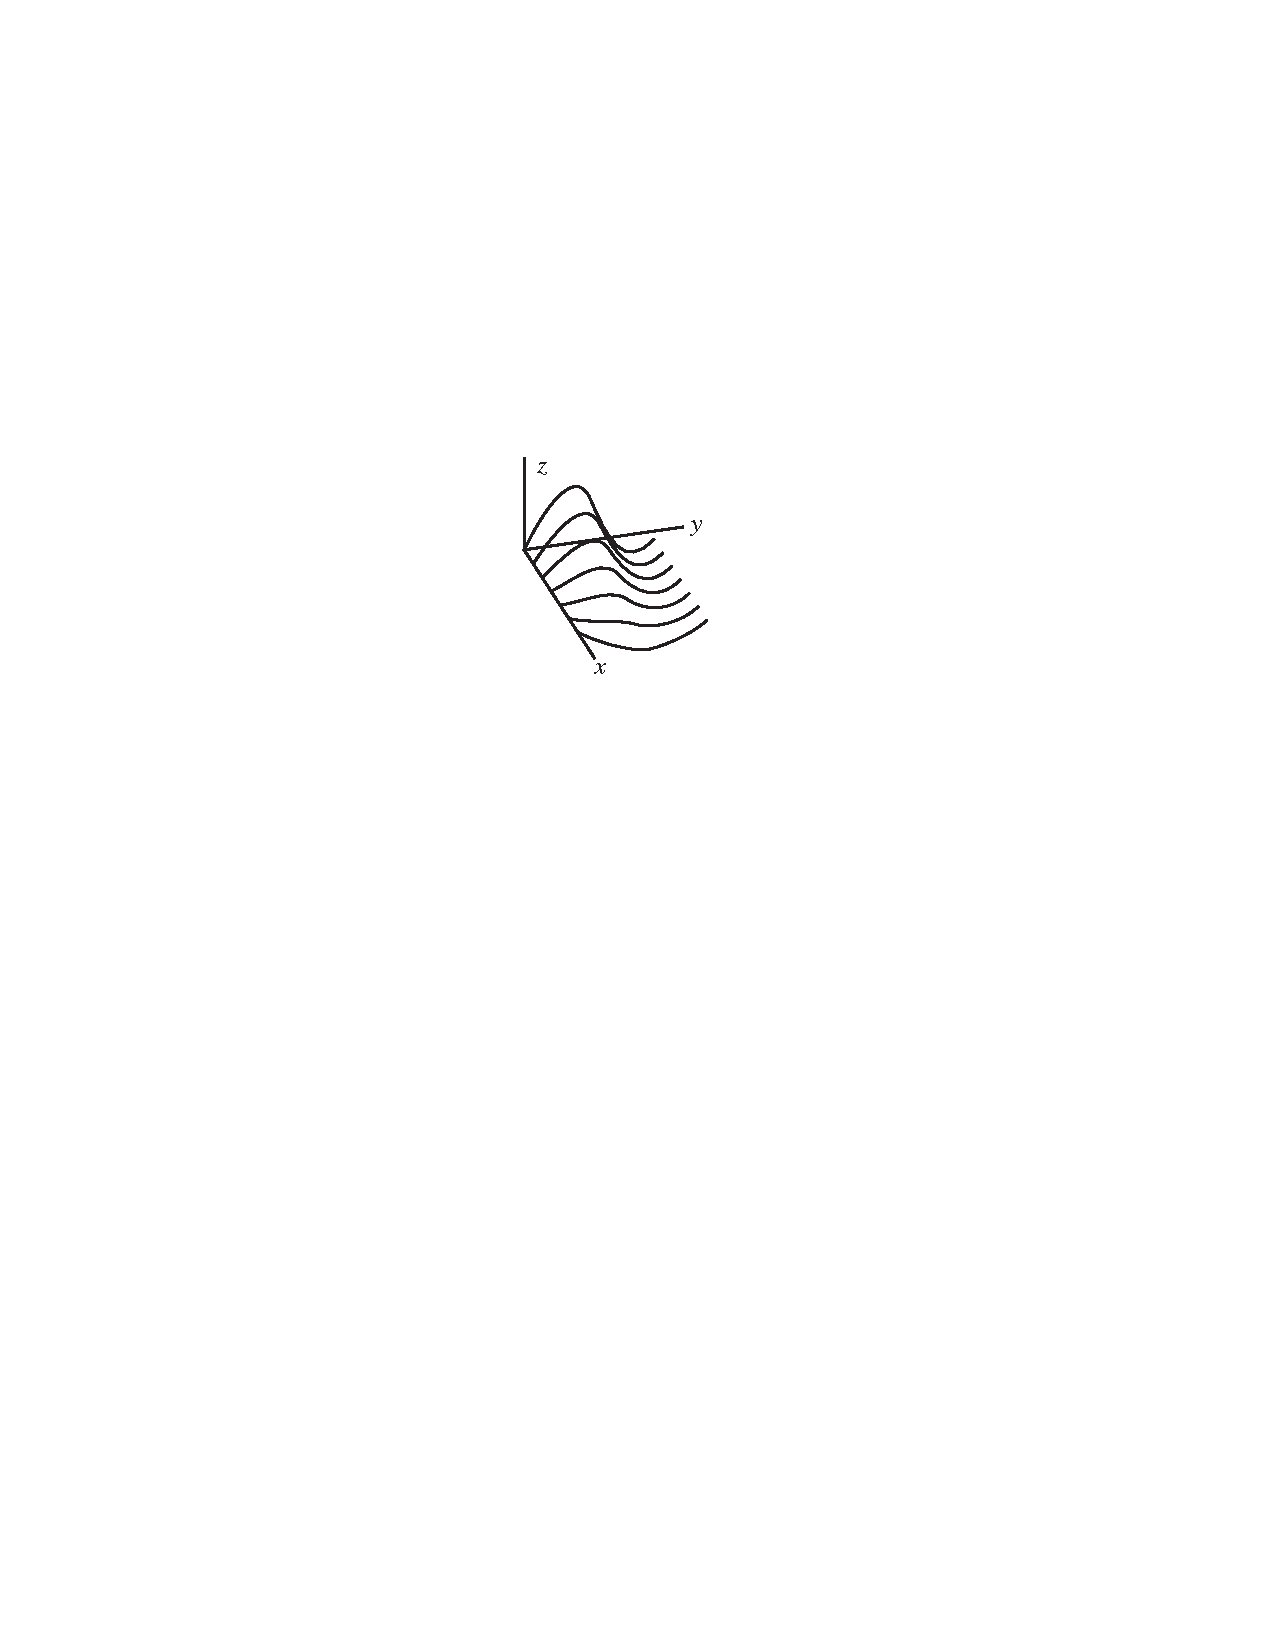
\includegraphics[scale=0.8]{01frozenvariable.pdf} }


\subsection{Moving graphs} 
There is another way of visualizing a function $z=f(x, y)$ of two variables in which we
think of one of the independent variables (e.g.~$y$) as ``time.''  The final picture
is not one static image of a three dimensional surface, but rather a movie of a
graph that is moving around in the $xz$ plane.

If we have a function $z=f(x, y)$, then let us think of $y$ as time, and let us
relabel it as $t$, so that we are looking at the function $z=f(x,t)$. Now at each
moment in time $t$ we can think of $z=f(x,t)$ as a function of one variable $x$ whose
graph we can try to draw, regarding it as a still-image.  Then, as we let time $t$
vary, putting the still images in a sequence, you get a movie of a graph of a
changing function of one variable.

\begin{figure}[b]
  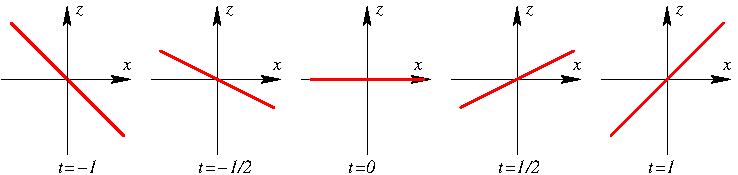
\includegraphics{01saddle-movie.pdf}
  \caption{The saddle movie. It's about a line segment whose slope changes, even
  though it is otherwise stuck to the origin.}
  \label{fig:saddle-movie}
\end{figure}

For instance, if the function is (once again) the saddle surface function $z=xy$,
then we would be considering the function $z=xt$.  At each moment $t$ the graph of
$z=xt$ is a line with slope $t$. Putting these graphs together gives a movie which
begins with a line of rather negative slope;  during the movie the slope increases,
and in the middle of the movie our line has achieved horizontality; finally, the
closing shot presents us with a line with a very positive slope.
Figure~\ref{fig:saddle-movie} shows some stills from the movie.

This interpretation is not very different from the procedure of ``freezing the $y$
variable.'' The only real difference lies in what we do with all the separate graphs
we get after we freeze a variable. In one case we try to piece them together to make
a bigger drawing of a three-dimensional object, in the other we put them together to
make a motion picture.


\section*{Problems} 
\label{sec:graphing-problems-2d3d}
\problemfont 
In the problems in this stage of the course, you will be asked to
``sketch the graph of a function.''  From math 221 you remember that
this meant you had to find minima, maxima, inflection points, and other
features of the graph.  In 234 you will learn to do the same for
functions of two (and more) variables, but for now you should try to
use the method of ``freezing a variable'' or other similar tricks to
get an idea of what the graph of $f$ looks like.

You can use a graphing program (such as \texttt{Grapher.app} on the
Mac, \texttt{GraphCalc} on Windows, or one of the many websites such as
\url{http://www.graphycalc.com/}) to check your answer.

\begin{center}
  \framebox{\parbox{0.4\textwidth}{Note: very often students try to
      fit their drawings into a region the size of a post-it.  In this
      course, whenever you make a drawing, especially if it's a
      three-dimensional drawing, \emph{make it large!}  Use half a
      page for a drawing.  Make sure you have enough paper, try to
      find lots of cheap scrap paper.}}
\end{center}
\begin{multicols}{2}
\problem If we were to drain Lake Mendota, 
as suggested in \S~\ref{sec:01mendotaexample}, would the lake bottom give us the
graph of $d(x, y)$ or of $-d(x,y)$?  (where $d$ is the depth of the lake)?
\answer
$-d(x,y)$.
\endanswer

\problem What are the signs of the coefficients $a$, $b$, and $c$ 
for the linear function whose graph is drawn in Figure~\ref{fig:graph-of-lin-f}?
\answer 
$a<0$, $b>0$, $c>0$.
\endanswer

\problem \itshape About planes and their intersections with the coordinate 
axes.\upshape

\subprob Where does the plane $z=3x-y+6$ intersect the three coordinate axes?
\answer
$x=-2$ for the $x$-axis, $y=6$ for the $y$-axis, $z=6$ for the $z$-axis.
\endanswer

\subprob Find the equation for the plane that intersects 
the $x$-axis at $x=4$, the $y$-axis at $y=2$, and the $z$-axis at $z=3$.
\answer
$z = 3 - \frac34 x - \frac32y$.
\endanswer

\subprob Find the equation for the plane that intersects 
the $x$-axis at $x=a$, the $y$-axis at $y=b$, and the $z$-axis at $z=c$.  (Write
the equation as nice as possible.)
\answer  
$\DS \frac{x}{a} + \frac{y}{b} + \frac{z}{c} = 1$ is a nice symmetric way of
writing the equation.
\endanswer

\problem Find a formula for the distance to the origin of the graph of 
\eqref{eq:linear-function}.
\answer
The distance is $\DS \frac{|c|}{\sqrt{1+a^2+b^2}}$.
\endanswer

\problem 
Classify the following quadratic forms as definite, indefinite, or other, by
completing the square.  Determine the zero set for each of these quadratic forms.

\subprob $f(x, y) = x^2+2y^2$
\answer
This one is already the sum of squares.  We don't have to do anything, and can
immediately conclude that $f(x, y)>0$ for all $(x,y)$ in the plane except the origin,
where $x=y=0$ and $f(x, y) = 0$.
\endanswer

\subprob $Q(x, y) = x^2-y^2$
\answer
The square containing $x$ is already complete (no $xy$ terms) and we can immediately
factor $Q(x, y) = (x-y)(x+y)$.
\endanswer

\subprob $g(x, y) = x^2-4xy + 3y^2$
\answer
We complete the square:
\[
  g(x, y) = (x-2y)^2 - y^2.
\]
We get the difference of two squares, so we can factor the quadratic form:
\[
  g(x, y) = (x-2y - y) (x-2y + y) = (x-3y)(x-y).
\]
\endanswer

\subprob $Q(s,t) = 9s^2-36st + 81t^2$
\answer
This one is positive definite:
\[
  Q 
  = 9\bigl( s^2 - 4st + 9 t^2\bigr)
  = 9\bigl[ (s - 2t)^2 -4t^2 + 9 t^2\bigr]
  = 9\bigl[ (s - 2t)^2 + 5 t^2\bigr]
  =9(s-2t)^2 + 45 t^2.
\]
\endanswer

\subprob $M(\alpha, \beta) = \frac12 \alpha^2 - \alpha\beta+\beta^2$.
\answer
Positive definite:
\[
  M = \frac12\bigl\{\alpha^2- 2\alpha\beta + 2\beta^2\bigr\}
  =\frac12 \bigl\{(\alpha-\beta)^2 + \beta^2\bigr\}.
\]
\endanswer

\subprob $Q(x,y) = xy+y^2$
\answer
This quadratic form has no $x^2$ term.  When that happens you cna immediately factor
the form, because all terms contain $y$:
\[
Q(x,y) = xy+y^2 = (x+y)y.
\]
This form is indefinite.
\endanswer

\subprob $Q(x, y) = x^2+2xy$
\answer
Now this form does have an $x^2$ term, so we \textit{can} complete the square if we
want to \dots but if we look carefully then we see that there's not $y^2$ term.
Because of this we can factor out $x$, and we get
\[
  Q = x^2+2xy = x(x+2y).
\]
The form is indefinite.

What if we don't notice that $y^2$ is missing and just blindly complete the square?
Nothing goes wrong and we get the same answer:
\[
  Q = x^2+2xy = x^2+ 2xy +y^2 - y^2 = (x+y)^2 - y^2 = (x+y - y)(x+y+y) = x(x+2y).
\]
We did work too hard though \verb|:-(|
\endanswer

\problem  For which values of the constant $k$ is the quadratic form
\[
  Q(x, y) = x^2 + 2kxy + y^2
\]
positive definite?
\answer
Complete the square:
\[
  Q=(x+ky)^2 - k^2 y^2 + y^2
   =(x+ky)^2 + (1- k^2) y^2.
\]
If $1-k^2>0$ then we have the sum of two squares.  If $1-k^2<0$, then we can rewrite
$Q$ as the difference of two squares
\[
   Q=(x+ky)^2 - (k^2-1) y^2
   =(x+ky)^2 - \bigl(\sqrt{k^2-1}y\bigr)^2
\]
which is indefinite.  That is all we need to know: we are not actually asked to
factor the form when it is indefinite.  But in case you're wondering, the somewhat
ugly formula is thus:
\[
  Q = \Bigl(x+(k+\sqrt{k^2-1}) y\Bigr) \Bigl(x+(k-\sqrt{k^2-1}) y\Bigr).
\]

The conclusion is that $Q(x,y)$ is positive definite if $-1<k<1$ and indefinite when
$k>1$ or $k<-1$.  In the remaining cases $k=\pm1$ we have
\[
  Q=(x+ky)^2 - k^2 y^2 + y^2
   =(x+ky)^2 + (1- k^2) y^2 = (x\pm y)^2,
\]
i.e.~ the form is a square (it is semidefinite).
\endanswer

\problem\label{prb:some-functions}
Which functions of two variables $z=f(x, y)$ are defined by the
following formulae?
\begin{trivlist}
\item[$\triangleright$] Find draw the domain of each function (the largest domain on
  which the definition would make sense).
\item[$\triangleright$] Try to sketch their graphs.
\item[$\triangleright$] Draw the level sets for each function.
\end{trivlist}

\subprob $z=xy$ 
\answer
The graph is the saddle surface, the function is defined at all $(x,y)$.  The level
set is given by $xy = c$.  If $c\ne 0$ then this set consists of both branches of the
hyperbola $y=\frac{c}{x}$.  If $c=0$ then $xy=0$ is equivalent with $x=0$ or $y=0$,
so the level set is the union of the $x$-and $y$-axes.
\endanswer
\subprob $z-x^2=0$ 
\answer
$z-x^2=0$.
Domain $\R^2$.  Graph is a \emph{parabolic cylinder} and consists of
horizontal lines perpendicular to the $xz$-plane, going through the
parabola $y=x^2$ in that plane.

Level sets: parallel straight lines $x=\pm\sqrt{z}$ if $z>0$,
the $x$ axis if $z=0$, the empty set if $z<0$.
\endanswer
\subprob $z^2-x=0$ 
\answer
$z^2-x=0$.
Implicit function.
At least two functions are defined, namely $z=\pm \sqrt{x}$.
Domain: all points $(x,y)$ with $x\ge 0$.
Graph is \emph{half a parabolic cylinder} and consists of
horizontal lines perpendicular to the $xz$-plane, going through the
parabola $z=\sqrt x$ (or $z=-\sqrt x$, depending on which function
you choose) in that plane.

Level sets (assuming we choose the function $z=+\sqrt{x}$):
the line $x=z^2$ if $z\ge0$, empty set otherwise.
\endanswer
\subprob $z-x^2-y^2=0$
\answer
$z-x^2-y^2=0$.
Domain is the whole plane.
Graph is a paraboloid of revolution, obtained by rotating the
parabola $z=x^2$ in the $xz$-plane around the $z$ axis.

Level sets: circle with radius $\sqrt{z}$ for $z>0$,
the origin for $z=0$ (note: this level set is a point rather than a curve),
empty for $z<0$.
\endanswer
\subprob $z^2-x^2-y^2=0$
\answer
$z^2-x^2-y^2=0$.
Implicit function.  Domain all of $\R^2$.
Possible functions are $z=\pm\sqrt{x^2+y^2}$.
Graph is the cone obtained by rotating the
half line $z=x, x\geq0$ in the $xz$-plane around the $z$ axis
(or the half line $z=-x, x\geq0$, if you chose $z=-\sqrt{x^2+y^2}$.)

Level sets (assuming we choose $z=+\sqrt{x^2+y^2}$):  circle with radius
$z$ when $z>0$, origin when $z=0$, empty when $z<0$.
\endanswer

\subprob $xyz=1$
\answer
$xyz=1$.
Domain the whole plain with the $x$ and $y$-axes removed, i.e.\ all
points $(x, y)$ with $xy\ne0$.
Function is $f(x, y) = \frac{1} {xy}$.
For each $y$ the graph is the hyperbola $z=1/(yx)$ which is just the
standard hyperbola $z=1/x$ stretched vertically by a factor $1/y$.
As $y\to 0$ this factor goes to $\infty$.
\endanswer

\subprob $xy/z^2=1$
\answer
$xy/z^2=1$.
Implicit function.
Domain first and third quadrants (all points with $xy>0$).
Functions $z= \pm \sqrt{xy}$.
Cross sections with planes $y=$constant are half parabolas.

Note: Harder to see, but the surface with equation $xy=z^2$ is in fact
the cone obtained by rotating the $x$-axis around the line
$x=y$ in the $xy$-plane.
\endanswer

\subprob $x+y+z^2=0$

\subprob $x+y+z^2=1$

\problem\label{prb:polar-angle-formula} 
The following expressions are all equal to the polar angle $\theta$ in some region of
the $xy$-plane.  Explain why the expression gives $\theta$, and identify in which
region this holds.

\subprob $\DS \theta = \arctan \frac{y}{x}$
\answer
$x>0$.  This one is in the text.
\endanswer

\subprob $\DS \theta = \frac\pi2 - \arctan \frac{x}{y}$
\answer
In the upper half plane, $y>0$.
\endanswer

\subprob $\theta=\arcsin \frac{y}{\sqrt{x^2+y^2}}$.
\answer
$x>0$.  
\endanswer

\problem {\itshape``The level set is always a curve\dots'' --- not!}\\ 
If $d(x, y)$ is the depth function of Lake Mendota (see
\S\ref{sec:01mendotaexample}), then what are the level sets $d^{-1}(c)$
for $c=0$, $c=+24$ and for $c=-24$ (meters)?  What is the level
set $d^{-1}(400)$ (meter)?
\answer 
The level set for $c=-24$ is the empty set, since it consists of all points on
the lake surface where the lake is $-24$ meters deep--i.e.~where the water
reaches $24$meters {\bfseries\itshape above} the lake.    

Similarly, the level set for $c=+400$ is also empty since the lake is not that
deep anywhere.

The level set $d^{-1}(0)$ consists of those points where the lake is $0$meters
deep.  This is exactly the shore line.

The level set $d^{-1}(24)$ consists of all points on the lake surface where the
lake is exactly $24$meters deep.  Form the map it looks like this happens on two
separate curves near the center of the lake.
\endanswer



\problem Describe and explain the relation between the graph of the 
function $y=g(x)$ of one variable, and the corresponding function
$f(x, y) = g\bigl( \sqrt{x^2+y^2} \bigr)$ of two variables.

What do the level sets of $f(x, y)$ look like?

For instance, if $g(x) = x$, then $f(x, y) = \sqrt{x^2+y^2}$: what is
the relation between the graphs of $g$ and $f$?
\answer
See \S~\ref{sec:functions-in-PC}.
\endanswer


\problem Find the largest domain on which 
the following functions of two (or occasionally three) variables can be defined:

\subprob  $f(x, y) = \sqrt{9-x^2}+\sqrt{y^2-4}$
\answer
The two rectangular strips $-3\leq x\leq3, 2\leq y<\infty$ and
$-3\leq x\leq3, -\infty<y\leq-2$.
\endanswer

\subprob  $f(x, y) = \arcsin(x^2+y^2-2)$
\answer
By definition $\arcsin(x)$ is only defined if $-1\leq x\leq1$.
For $\arcsin(x^2+y^2-2)$ to be defined, we must therefore have
$-1\leq x^2+y^2-2 \leq 1$, i.e.\ $1\leq x^2+y^2 \leq 3$.

The domain of this function is
the ring-shaped region between the circles with radii $1$ and
$\sqrt{3}$, both centered at the origin.
Circles are included in the domain.
\endanswer

\subprob  $f(x, y) = \sqrt{x}\;\cdot\;\sqrt{y}$
\answer
The way this function is written both $\sqrt x$ and $\sqrt y$ must be defined,
so the domain consists off all $(x,y)$ with $x\geq0$ and $y\geq0$.
\endanswer

\subprob  $f(x, y) = \sqrt{xy}$
\answer
$\sqrt{xy}$ must exist, which happens for all $(x,y)$ in the first
and third quadrants (axes included.)
\endanswer

\subprob  $f(x, y, z) = 1/\sqrt{xyz}$

\subprob  $f(x, y) = \sqrt{16-x^2-4y^2}$
\answer
The region in the plane given by $x^2+4y^2\leq16$, which is the region
enclosed by an ellipse with
major axis of length 4, along the $x$ axis, and minor axis of length
2 along the $y$-axis.  The ellipse is included.
\endanswer

\problem\label{prb:cone-or-paraboloid}
Here are two sets of level curves with levels $z=0.2, 0.4, 0.6, 0.8,
1.0, 1.2,  1.4$.  One is for a function whose graph is a cone
($z=\sqrt{x^2+y^2}$), the other is for a paraboloid ($z=x^2+y^2$).
Which is which? Explain.
\answer
The level sets of the function whose graph is a cone are equally spaced circles
(the level set at level $c$ is a circle with radius $c$).  Hence the one on the
right corresponds to the cone, and
the one on the left corresponds to the paraboloid.
\endanswer
\begin{center}
  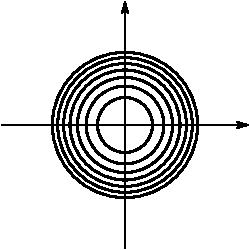
\includegraphics[scale=0.7]{01paraboloidLevels.pdf}
  \quad
  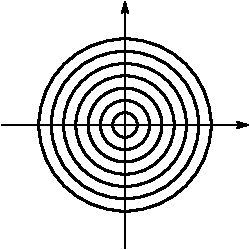
\includegraphics[scale=0.7]{01coneLevels.pdf}
\end{center}

\problem\label{prb:distance-to-square-level-sets}
\carefulnow~
Let $Q$ be the square in the plane consisting of all points $(x,y)$
with $|x|\le1$, $|y|\le1$.  This problem is about the so-called
\emph{distance function} to $Q$.  This function is defined as
follows:  $f(x, y)$ is the distance from the point $(x,y)$ to the
point in $Q$ nearest to $(x,y)$.

\subprob Which point in $Q$ is nearest to $(0, \frac12)$?  Which is
closest to $(0, 2)$?  Which is closest to $(3,4)$?
\answer
$(0, \frac{1} {2})$ is in the square $Q$, so it is the point closest to
$(0, \frac{1} {2})$.\\
The point $(0,1)$ on the top edge of the square is closest to $(0,2)$.\\
The corner point $(1,1)$ is closest to $(3,4)$.
\endanswer

\subprob Compute $f(0, \frac12)$, $f(0,2)$ and $f(3, 4))$.
\answer
$f(0, \frac12) =0 $;
$f(0,2)=1$ and $f(3, 4))=\sqrt{2^2+3^2}=\sqrt{13}$.
\endanswer

\subprob What is the zero set of $f$?
\answer
The zero set of $f$ is the square $Q$.
\endanswer

\subprob Draw the level sets of $f$ at levels $-1$, 1, 2, and 3.  Describe
the general level set $f(x, y) = c$ where $c$ is an arbitrary number.
\answer
The level set at level $-1$ is empty.  The others are ``rounded
rectangles,'' see this drawing, in which the square is grey, the dashed
lines are given by $x=\pm1$ or $y=\pm1$.
\begin{center}
    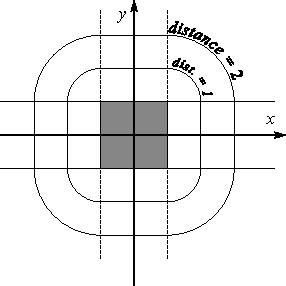
\includegraphics{01distancetosquare.pdf}
\end{center}
\endanswer

\subprob Give a formula for $f(x, y)$.  (It turns out to be too hard to
capture the distance function in one formula.  You will have to split the
plane into different regions and describe $f(x,y)$ by different formulas,
according to which region $(x,y)$ belongs to.)
\answer
The lines $x=\pm1$ and $y=\pm1$ divide the plane into nine regions.
On each region the function is given by a different formula.
Here they are:
\begin{tabbing}
\=$\boldmath{f(x, y)}$ \=\`\textbf{ if } \ldots \\
\>$0$  \>\` $(x, y)$ in $Q$\\
\>$x-1$ \>\` $x\geq1, |y|\leq 1$\\
\>$y-1$ \>\` $|x|\leq 1, y\geq1$\\
\>$-x-1$ \>\` $x\le-1, |y|\leq 1$\\
\>$-y-1$ \>\` $|x|\leq 1, y\le-1$\\
\>$\sqrt{(x-1)^2+(y-1)^2}$ \>\` $x\ge1$ and $y\ge1$\\
\>$\sqrt{(x-1)^2+(y+1)^2}$ \>\` $x\ge1$ and $y\le-1$\\
\>$\sqrt{(x+1)^2+(y-1)^2}$ \>\` $x\le-1$ and $y\ge1$\\
\>$\sqrt{(x+1)^2+(y+1)^2}$ \>\` $x\le-1$ \& $y\le-1$\\
\end{tabbing}
\endanswer

\problem  Describe the ``movie'' that goes with each of the following 
functions.

\subprob $f(x, t) = x\sin t$
\answer
At time $t$ we have a line through the origin with slope $\sin t$.
As time progresses this lines turns up and down, and up and down,  etc.
\endanswer
\subprob $f(x, t) = x\sin 2t$
\answer
Same as previous problem, but twice as fast.
\endanswer

\subprob $f(x, t) = t\sin x$
\answer
At all times one sees the graph of $y=\sin x$ stretched vertically by a factor $t$.
\endanswer

\subprob $f(x, t) = 2t \sin x$
\answer
Same as previous problem, but twice as fast.
\endanswer
\subprob $f(x, t) = t\sin 2x$
\answer
The graph of $y=\sin 2x$ stretched vertically by a factor $t$.
\endanswer

\subprob $f(x, t) = (x-t)^2$
\answer
Parabola with its minimum on the $x$-axis at $x=t$.
So we see the parabola $y=x^2$ translating from the left to the right
with constant speed 1.
\endanswer

\subprob $f(x, t) = (x-\sin t)^2$
\answer
Parabola with its minimum on the $x$-axis at $x=\sin t$.
So we see the parabola $y=x^2$ translating back and forth horizontally
every $2\pi$ time units.
\endanswer

\subprob $f(x, t) = (x-t^2)^2$

\subprob $f(x, t) = \dfrac{t^2}{1+x^2}$

\subprob $f(x, t) = \dfrac{1}{(1+x^2) (1+t^2)}$
\answer
At time $t$ we see Agnesi's witch, i.e. the graph $y= a/(1+x^2)$
with amplitude $a=1/(1+t^2)$.  Thus we see a bump whcich starts out small
 at $t=-\infty$, grows to its maximal size at time $t=0$, and then decays
again, until it vanishes at $t=+\infty$.
\endanswer

\problem Describe the movie that goes with the function
\[
  f(x, t) = \arctan \frac xt,
\]
for $t>0$.  The function is not defined at $t=0$, but can you describe the limit
of this function as $t\to0$?  (Hint: the sign of $x$ matters).


\problem \label{prb:01traveling-waves}
If $y=g(x)$ is any function of one variable, then a function of the
form $f(x, t) = g(x-vt)$ is often called a \emph{traveling wave} with
wave speed $v$ and profile $g$.  Let $g$ be any non constant
function of your choice and describe the movie presented by the
function $f(x, t) = g(x-vt)$ (can't choose?  Then try ``Agnesi's
witch'' $g(x) = \frac{1}{1+x^2}$.)

The number $v$ is called the wave speed.  If $v>0$ is the motion to
the left or to the right? Explain.
\answer
The graph of $y=g(x-a)$ is obtained from the graph of $y=g(x)$ by
translating the graph of $y=g(x)$ by $a$ units to the right.

Hence the graph of $g(x-vt)$ is the graph of $g(x)$ translated by $vt$
units to the right.  As time changes the graph of $g(x-vt)$ therefore
moves with velocity $v$ to the right.
\endanswer


\problem If $y=g(x)$ is any function of one variable, then a function 
of the form
\[
  f(x, t) = \cos(\omega t) g(x)
\]
is often called a \emph{standing wave.}
Let $g$ be any non constant function of your choice and describe the
movie presented by the function $f(x, t) = \cos(\omega t)g(x)$
(can't choose?  Then try ``Agnesi's witch''  $g(x) = \frac{1}{1+x^2}$
again, or for this example, try $g(x) = \sin x$.)

The number $\frac\omega{2\pi}$ is called the frequency of the standing
wave.  The function $g(x)$ is called its profile.  How long does it
take before the standing wave returns to its original position, i.e.\
what is the smallest $T>0$ for which $f(x, T) = f(x, 0)$ for all $x$?
Explain.
\answer
If you know the graph of a function $y=g(x)$, then you get
the graph of $y=cg(x)$ by stretching the graph of $g$ vertically by
a factor $c$ (here $c$ is a constant.)
If you allow this constant to depend on time, e.g.\ as in this
problem by setting $c=\cos(\omega t)$, then the ``movie'' you get is of a
version of the graph of $g$ which is growing and shrinking vertically.

\begin{center}
    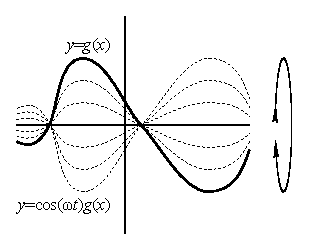
\includegraphics{01standingwave.pdf}
\end{center}
\endanswer
\end{multicols}
\noproblemfont


%%% Local Variables: 
%%% mode: latex
%%% TeX-master: "free234"
%%% End: 

% !TEX root =free234.tex
% Time-stamp: <2015-10-23 13:07:31 angenent>
\chapter{Derivatives}

\section{Interior points and continuous functions} 
Before diving into the calculus of partial derivatives we need to discuss certain
assumptions that we shall always implicitly make about the functions in this course.
The first concerns the domains of our functions.  Namely:
\begin{equation}
  \text{\itshape We only consider functions at interior points of their domain}
  \label{eq:domains-are-open}
\end{equation}
Here, by definition, a point $(a,b)$ in the domain of a function is called an
\textit{interior point} if the function is also defined at all points $(x,y)$
that lie within some small disc centered at $(a,b)$.
\begin{figure}[h]
  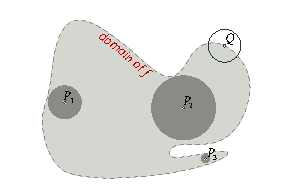
\includegraphics[width=0.6\textwidth]{01domain-is-open.pdf}
  \caption{\textbf{Interior and boundary points in the domain of $f$:} $P_1$,
    $P_2$, or $P_3$ are interior points in the domain. Each of these points is
    the center of a sufficiently small disc that is still contained in the
    domain.  For points such as $Q$, that lie on the edge of the domain, any
    disc centered at $Q$ will ``stick out of the domain,'' no matter how small
    the disc is chosen.  If we talk about the derivative of a function at some
    point in its domain, then, \textit{in this course}, we will always assume
    that we are not at an edge-point like $Q$.}
  \label{fig:domain-is-open}
\end{figure}

The other standing assumption we make in this course is that
\begin{equation}
  \text{\itshape all functions we consider are continuous.}
  \label{eq:all-functions-continuous}
\end{equation}
We have seen the concept of continuity for functions of one variable.  For
functions of more variables ``continuity'' has a similar definition. In this
course we will aim for an intuitive understanding of the concept, which can be
formulated as follows.
\begin{quote}
  \itshape%
  The function $z=f(x, y)$ is continuous at some point $(a,b)$ if the function
  value $f(x, y)$ at any point $(x,y)$ is close to $f(a, b)$ when $(x,y)$ is
  close to $(a,b)$.
\end{quote}
There are many other ways of describing continuity, e.g.~one can say that $f$ is
continuous at $(a,b)$ if
\[
\lim_{(x,y)\to(a,b)} f(x,y) =f(a,b).
\]
To make this precise we would have to define what ``$\lim_{(x,y) \to
  (a,b)}\dots$'' means.

A precise definition of ``$f$ is continuous at $(a,b)$'' invokes $\varepsilon$'s
and $\delta$'s:
\begin{quote}
  \itshape%
  The function $z=f(x, y)$ is continuous at some point $(a,b)$ if for every
  $\varepsilon>0$ there is a $\delta>0$ such that for every point $(x,y)$ that
  lies in the disc of radius $\delta$ centered at $(a,b)$ one has $|f(x,y) -
  f(a,b)| < \varepsilon$.
\end{quote}
In this course we will not use the definition much, but we will occasionally
appeal to the intuitive notion of ``continuity.''  The problems show some
examples of how a function of two variables can fail to be
continuous (e.g.~Problem~\ref{prb:some-discontinuous-functions}).

Now that we have dispensed with these preliminary issues, we can go on to the
central topic in the first half of the semester: partial derivatives and the
chain rule.

\section{Partial Derivatives}        
The derivative $f'(x)$ of a function of one variable, $y=f(x)$, measures a rate
of change: if we increase $x$ by a small amount $\Delta x$ then $y=f(x)$ also
increases by a small amount $\Delta y$.  The ratio between these two changes is
the derivative: $f'(x) \approx \frac{\Delta y}{\Delta x}$.

For a function $z=f(x, y)$ of two variables there is a similar concept: if we
change $x$ and/or $y$ by a small amount then $z$ will also change by a small
amount, and there are formulas relating the changes $\Delta x$, $\Delta y$ and
$\Delta z$.  Because there are many different ways in which we can change $x$
and $y$ there are a few different formulas.  We will encounter the following
versions of ``the derivative of $f(x, y)$'':

\textcolor{badgerred}{$\blacktriangleright$} Change only one of the variables
but not the other: this leads to the so-called \emph{partial derivatives}.

\textcolor{badgerred}{$\blacktriangleright$} Simultaneously vary both $x$ and
$y$: the resulting change turns out to be the sum of the changes we would get if
we were to vary only $x$ or only $y$, respectively.  This will follow from the
\emph{chain rule}, and the resulting formula is called the \emph{total
  derivative}.

We begin with the partial derivatives.

\begin{definition}[Definition of Partial Derivatives]
  If $z=f(x, y)$ is a function of two variables then the partial derivatives of
  $f$ with respect to $x$ and with respect to $y$ are
  \begin{equation}\label{eq:partial-wrt-x-defined}
    \pdd fx(x, y)
    = \lim_{\Delta x\to 0}
    \frac{f(x+\Delta x, y) - f(x, y)}{\Delta x}
  \end{equation}
  and
  \begin{equation}\label{eq:partial-wrt-y-defined}
    \pdd fy(x, y)
    = \lim_{\Delta y\to 0}
    \frac{f(x, y+\Delta y) - f(x, y)}{\Delta y}
  \end{equation}
\end{definition}


\begin{figure}[h]\flushleft
  \def\verticalderivativetext{\dfnt$\dfrac{\partial f}{\partial y}$ is the rate
    of change of $f$ in the vertical direction}
  \def\horizontalderivativetext{\dfnt$\dfrac{\partial f}{\partial x}$ is the
    rate of change of $f$ in the horizontal direction}
  \def\domaintext{\parbox{3in}{\dfnt When we define the partial derivatives at
      some point $(x,y)$, we assume that the function is defined on some
      sufficiently small disc centered at that point $(x,y)$. }} \input
  ../figures/234/02domain-for-partial-derivs.pdf_tex
  \caption{The partial derivatives of a function at some point $(x,y)$ measure
    how fast the function $f(x,y)$ changes if we move the point either
    horizontally (the $x$ direction) or vertically (the $y$ direction).  }
  \label{fig:about-the-partials}
\end{figure}

The following more convenient notation is used very often (because it's so much
shorter):
\begin{equation}
  f_x(x, y) = \pdd fx(x,y),\qquad
  f_y(x, y) = \pdd fy(x,y).
\end{equation}
When we are in a hurry we can also drop the ``$(x, y)$'' from our notation for
derivatives and just write $f_x$ and $f_y$.

\subsection{Partial derivatives of functions of three or more variables} 
If a function depends on three or more variables then one can define its partial
derivatives in the same way as for functions of two variables.  For instance, if
$w=f(x, y, z)$ is a function of three variables, then its partial derivative
with respect to $x$ is defined to be
\[
\pdd fx = \lim_{\Delta x\to0} \frac{f(x+\Delta x, y, z) - f(x, y, z)}{\Delta x}.
\]
The derivatives of $f$ with respect to $y$ and $z$ have very similar
definitions.

\subsection{Examples}
\label{sec:partial-derivatives-examples}
Computing partial derivatives is not harder than computing ordinary derivatives.
To find the partial derivative of a function with respect to $x$ we just pretend
all other variables are constants and differentiate.  Or, in other words, we
could think of the partial derivative of $f(x,y)$ with respect to $x$ as the
ordinary derivative of the function $f$ in which we have frozen the variable $y$
at some particular value.

For instance, the partial derivatives of the function $f(x, y, z) = x^2\sin\pi
y+z$ of \emph{three} variables $x$, $y$, and $z$, are
\[
f_x = 2x\sin\pi y,\quad f_y = \pi x^2\cos\pi y\text{ and } f_z = 1.
\]


\section{Problems}
\label{sec:partial-derivative-problems}
\begin{multicols}{2}
  % \immediate\write\ans{\string\newpage}
\problemfont
\problem \label{prb:some-discontinuous-functions}
For each of the following functions sketch the graph (use a graphing program, if
necessary) and decide if you think the function has a limit as $(x,y)$
approaches $(0,0)$.

\subprob $\DS f(x,y) = \frac{xy}{x^2+y^2}$

\subprob $\DS g(x, y) = \frac{1}{x^2+y^2}$

\subprob $\DS h(x, y) = \frac{x}{x^2+y^2}$.

\subprob $\DS p(x, y) = \frac{x}{\sqrt{x^2+y^2}}$.

\subprob $\DS q(x, y) = \frac{x^2}{\sqrt{x^2+y^2}}$.


\problem\label{prb:01compute-these-partials}
Find the partial derivatives of the following functions:

\subprob 
$\DS f(x,y)=x^2y^3-x^3y^2$.

\subprob 
$\DS f(x,y)=\cos(x^2y)+y^3$.
\answer
$-2xy\sin(x^2y)$, $-x^2\sin(x^2y)+3y^2$
\endanswer

\subprob $\DS f(x,y)={xy\over x^2+y}$.
\answer
$(y^2-x^2y)/(x^2+y)^2$, $x^3/(x^2+y)^2$
\endanswer

\subprob $\DS f(x, t) = (x+t)^4$.

\subprob $\DS f(x, t) = (x-t)^4$.

\subprob $\DS f(x, t) = \sin\omega t \cos\frac{2\pi x}{L}$.

\bigskip

\subprob $\DS f(x,y)=e^{x^2+y^2}$.
\answer
$2xe^{x^2+y^2}$, $2ye^{x^2+y^2}$
\endanswer

\subprob $\DS f(x,y)=xy\ln(xy)$.
\answer
$y\ln(xy)+y$, $x\ln(xy)+x$
\endanswer

\subprob $\DS f(x,y)=\sqrt{1-x^2-y^2}$.
\answer
$-x/\sqrt{1-x^2-y^2}$, $-y/\sqrt{1-x^2-y^2}$
\endanswer

\subprob $\DS f(x, y, z) = \sqrt{x^2 + y^2 + z^2}$

\subprob $\DS f(u,v) = e^{u+v}$

\subprob $\DS f(x,y)=x\tan(y)$.
\answer
$\tan y$, $x/\cos^2 y$
\endanswer

\subprob $\DS f(x,y)={1\over xy}$.
\answer
$-1/(x^2y)$, $-1/(xy^2)$
\endanswer

\problem \label{prb:derivative-of-radius}% 
Let $r$ be the radius in polar coordinates, as defined in
\S~\ref{sec:functions-in-PC} of Chapter III.

\subprob Compute the partial derivatives of $r$.

\subprob Show that the partial derivatives of $r$ can be written as
\[
\pdd rx = \frac xr, \quad
\pdd ry = \frac yr.
\]

\problem \label{prb:derivative-of-theta}% 
Let $\theta$ be the polar angle function, defined in
\S~\ref{sec:functions-in-PC-theta} of Chapter III.

\subprob In the left half plane the function $\theta$ is defined by
\[
\theta(x,y) = \arctan\frac{y} {x}.
\]
Use this expression to find its partial derivatives, $\pdd\theta x$ and $\pdd\theta y$.
\answer
$\DS\pdd\theta x = -\frac{y} {x^2+y^2}$, $\DS\pdd\theta x = \frac{x} {x^2+y^2}$.
\endanswer

\subprob Check that the angle function also satisfies
\[
x\sin\theta = y\cos \theta
\]
at all points in the plane.  Use implicit differentiation to find the partial
derivatives $\pdd\theta x$ and $\pdd\theta y$.


\problem Let $f(x, y) = $ the distance from $(x,y)$ to the origin. 
Find a formula for $f$, and compute
\[
f_x, \quad f_y, \text{ and } \sqrt{f_x^2 +f_y^2}.
\]
(Hint: compare this problem with problem \ref{prb:derivative-of-radius}.)
\answer
The distance to the origin is exactly the radius in polar coordinates, so
$f(x, y) = \sqrt{x^2+y^2}$, and
\[
f_x = \frac{x} {\sqrt{x^2+y^2}},\qquad
f_y = \frac{y} {\sqrt{x^2+y^2}}.
\]
This is the same as in problem~\ref{prb:derivative-of-radius}.  The only
quantity that we did not compute before is
\[
\bigl(f_x\bigr)^2 + \bigl(f_y\bigr)^2 = \frac{x^2} {x^2+y^2} + \frac{y^2}
{x^2+y^2} = \frac{x^2+y^2} {x^2+y^2} = 1.
\]
\endanswer

\problem Suppose $f(t)$ and $g(t)$ are single variable differentiable 
functions.  Find $\partial z/\partial x$ and
$\partial z/\partial y$ for each of the following two variable functions.

\subprob  $z=f(x)g(y)$
\answer
$\frac{\pd z}{\pd x} = f'(x)g(y)$, 
$\frac{\pd z}{\pd y} = f(x)g'(y)$.
\endanswer

\subprob  $z=f(xy)$
\answer
$\frac{\pd z}{\pd x} = yf'(xy)$, 
$\frac{\pd z}{\pd y} = xf'(xy)$.
\endanswer

\subprob  $z=f(x/y)$
\answer
$\frac{\pd z}{\pd x} = \frac{1}{y}\, f'(\frac xy)$, 
$\frac{\pd z}{\pd y} = -\frac{x}{y^2} \, f'(\frac xy)$.
\endanswer

\problem
\label{prb:distance-to-square-partialderivs}
Let $f$ be the \emph{distance to the square $Q$ function} from
problem \ref{prb:distance-to-square-level-sets}.  Find the partial
derivatives $f_x$ and $f_y$ of $f$.  (You will need your answer to
problem \ref{prb:distance-to-square-level-sets}, in particular the
description of $f$ as a ``piecewise defined function''.)


\end{multicols}

\section{The linear approximation to a function}
\label{sec:the-linear-approximation-of-a-function}

\subsection{The Chain Rule and friends}     
When we compute the partial derivative of a function with respect to a variable
$x$ we pretend all other variables are constants, and just differentiate with
respect to $x$, just as we would in first semester calculus.  There is therefore
no need to state a product rule or quotient rule, because these are
\textit{exactly the same} as for functions of one variable.  The chain rule on
the other hand is different: there is a chain rule for functions of several
variables, but it has more terms than the chain rule from one-variable calculus.
There are several related topics that fit together in a discussion of the chain
rule, namely \emph{Linear Approximation}, \emph{Tangent Planes to a Graph}, and
\emph{The Total Derivative}.  We will go through these one at a time in the next
few sections.


\subsection{The linear approximation formula}
\label{sec:linear-approximation-no-error}
The key to the chain rule is the linear approximation formula.  This formula
tells us approximately how much a function $z=f(x, y)$ of two variables changes
if both variables are subjected to a small change.

More precisely, if we have a function $z=f(x,y)$, and we know its value
$f(x_0,y_0)$ at some point $(x_0,y_0)$, then how much does the function value
change if $x$ is increased from $x_0$ to $x_0+\Delta x$, and if $y$ is similarly
increased from $y_0$ to $y_0+\Delta y$?
\begin{figure}[h]

  \parbox{0.4\textwidth}{\input ../figures/234/01chainrule.pdf_tex}
  \hfill
  \parbox{0.59\textwidth}{\dfnt%
    We can change $(x_0,y_0)$ to $(x_0+\Delta x, y_0+\Delta y)$ in
    two steps: \\
    \null\quad first keep $y$ fixed and increase $x$ by $\Delta x$,\\
    \null\quad then keep $x$ fixed and increase $y$ by $\Delta y$}
 
  \parbox{0.4\textwidth}{\input ../figures/234/01chainrule-mvt-points.pdf_tex}
  \hfill
  \parbox{0.59\textwidth}{\dfnt%
    To express the change in function values in terms of derivatives, we can use
    the Mean Value Theorem.   We get two intermediate points:\\
    \null\quad one at $x=\tilde x$ for the increase in $f$ when $x$ changes, and\\
    \null\quad one at $y=\tilde y$ for the increase in $f$ when $y$ changes.}
 
  \caption{Computation of the linear approximation
    \eqref{eq:linear-approx-derivation} }
  \label{fig:computation-of-linear-approximation}
  % we compute the change in
  % function value when we go from $(x_0, y_0)$ to $(x_0+\Delta x, y_0+\Delta
  % y)$
  % by adding the change that occurs when we first go from $(x_0, y_0)$ to
  % $(x_0+\Delta x, y_0)$, and then from $(x_0+\Delta x, y_0)$ to $(x_0+\Delta
  % x,
  % y_0+\Delta y)$.
\end{figure}

% The quick version
The basic idea in the computation of the change in $f(x, y)$ is to go from
$(x_0,y_0)$ to $(x_0+\Delta x, y_0+\Delta y)$ in two steps:
\begin{align}
  \label{eq:linear-approx-derivation}
  \Delta f & = f(x_0+\Delta x, y_0+\Delta y) - f(x_0, y_0)\\
  &= \underbrace{f(x_0+\Delta x, y_0+\Delta y) - f(x_0+\Delta x, y_0)}
  _{\text{only $y$ changes}} + \underbrace{f(x_0+\Delta x, y_0) - f(x_0,
    y_0)}_{\text{only $x$ changes}} \nonumber
\end{align}
We have written the total change in $f$ as the sum of two changes, one of them
caused by the change in $x$, and the other due to the change in $y$.  See
Figure~\ref{fig:computation-of-linear-approximation}.

In the second difference only $x$ changes while $y$ remains the same, so we can
use the one variable Mean Value Theorem to conclude that there is some number
$\tilde x$ between $x_0$ and $x_0+\Delta x$ with
\[
\frac{f(x_0+\Delta x, y_0) - f(x_0, y_0)}{\Delta x} = f_x(\tilde x, y_0),
\]
i.e.
\begin{equation}
  f(x_0+\Delta x, y_0) - f(x_0, y_0) = f_x(\tilde x, y_0) \cdot \Delta x.
  \label{eq:change-caused-by-Dx}
\end{equation}
Likewise, in the difference in \eqref{eq:linear-approx-derivation} where only
$y$ changes we can use the Mean Value Theorem to conclude that there is some
$\tilde y$ between $y_0$ and $y_0+\Delta y$ such that
\[
\frac{f(x_0+\Delta x, y_0+\Delta y) - f(x_0+\Delta x, y_0)}{\Delta y} =
f_y(x_0+\Delta x, \tilde y),
\]
and hence
\begin{equation}
  f(x_0+\Delta x, y_0+\Delta y) - f(x_0+\Delta x, y_0) 
  = f_y(x_0+\Delta x, \tilde y) \cdot \Delta y.
  \label{eq:change-caused-by-Dy}
\end{equation}
If we now combine \eqref{eq:change-caused-by-Dx} and
\eqref{eq:change-caused-by-Dy} with \eqref{eq:linear-approx-derivation} then we
get
\[
\Delta f = f_x(\tilde x, y_0)\cdot\Delta x + f_y(x_0+\Delta x,\tilde
y)\cdot\Delta y.
\]
This equation is exactly true, i.e.~we have not made any approximations, and we
have not ignored any kind of ``error terms.''  However, the equation does
contain the numbers $\tilde x$ and $\tilde y$, which are provided by the Mean
Value Theorem, and of which we therefore do not know anything besides the fact
that $\tilde{x}$ lies between $x_0$ and $x_0 + \Delta x$, and $\tilde{y}$ lies
between $y_0$ and $y_0+\Delta y$.  We can get rid of this uncertainty by
settling for an approximation for $\Delta f$ instead of the exact expression we
have just found.  To do this we assume that $\Delta x$ and $\Delta y$ are
``small.''  Then, since $\tilde{x}$ lies between $x_0$ and $x_0+\Delta x$, we
know that $\tilde x\approx x_0$.  We also know that $y_0+\Delta y \approx y_0$,
so, if the function $f_x$ is continuous, then it seems reasonable to assume that
\begin{equation}
  f_x(\tilde{x}, y_0+\Delta y) \approx f_x(x_0, y_0).
  \label{eq:fx-continuous}
\end{equation}
Similarly, we will assume that
\begin{equation}
  f_y(x_0, \tilde{y}) \approx f_y(x_0, y_0).
  \label{eq:fy-continuous}
\end{equation}
Substituting this in \eqref{eq:linear-approx-derivation} we find
\begin{equation}
  \Delta f \approx f_x(x_0, y_0)\Delta x + f_y(x_0, y_0) \Delta y
  \label{eq:linear-approximation-no-error-Deltaf}
\end{equation}
Keeping in mind that $\Delta f = f(x_0+ \Delta x, y_0+\Delta y)-f(x_0,y_0)$, we
conclude
\begin{equation}
  \label{eq:linear-approximation-no-error}
  f(x_0+\Delta x, y_0+\Delta y)
  \approx
  f(x_0, y_0)+f_x(x_0, y_0)\Delta x + f_y(x_0, y_0) \Delta y
\end{equation}

The linear approximation formula \eqref{eq:linear-approximation-no-error} is
often written using Leibniz-style notation for the derivatives, where one writes
$\pdd fx$ for $f_x$, and $\pdd fy$ for $f_y$.  In this notation the
approximation formula takes these forms:
\[
f(x_0+\Delta x, y_0+\Delta y) \approx f(x_0, y_0) + \pdd fx(x_0, y_0)\cdot
\Delta x + \pdd fy(x_0, y_0)\cdot \Delta y,
\]
or, shorter,
\begin{equation}
  \Delta f \approx \pdd fx \Delta x + \pdd fy \Delta y.
  \label{eq:linear-approximation-Leibniz-notation}
\end{equation}

The approximation \eqref{eq:linear-approximation-no-error} can also be written
without $\Delta x$ and $\Delta y$ by a change of notation.  To do this we
introduce
\begin{equation}
  x = x_0 + \Delta x  \text{ and } y = y_0 + \Delta y,
  \label{eq:dxdy-and-xx0-yy0-relation}
\end{equation}
and interpret \eqref{eq:linear-approximation-no-error} as a formula that tells
us approximately what the function value at $(x,y)$ is, provided $(x,y)$ is
close enought to $(x_0,y_0)$.  Written in terms of $x$ and $y$,
\eqref{eq:linear-approximation-no-error} says
\begin{equation}
  f(x,y)
  \approx
  f(x_0, y_0)+f_x(x_0, y_0)\, (x-x_0) + f_y(x_0, y_0) \, (y-y_0).
  \label{eq:linear-approximation-no-error-no-dxdy}
\end{equation}

\subsection{Linear approximation -- infinitesimal version}
\label{sec:linear-approximation-infinitesimal}
We expect the approximation in \eqref{eq:linear-approximation-Leibniz-notation}
to improve as we decrease $\Delta x$ and $\Delta y$ (and we will try to make
this statement more precise in the next section,
\S~\ref{sec:linear-approximation-with-error}).  We could then say, as is
commonly done, that there is an exact equation when $\Delta x$ and $\Delta y$
are ``infinitely small,'' and write this equation as
\begin{equation}
  \label{eq:linear-approximation-infinitesimal}
  df = \pdd fx dx + \pdd fy dy.
\end{equation}
The meaning of this equation is that infinitesimally small changes in $x$ and
$y$, of magnitudes $dx$ and $dy$, respectively, lead to an infinitesimally small
change in $f$ of magnitude $df$, and that $df$, $dx$, and $dy$ are related by
\eqref{eq:linear-approximation-infinitesimal}.  Even though it is very difficult
to make sense of the ``infinitely small'' quantities $dx, dy, df$, in
\eqref{eq:linear-approximation-infinitesimal}, this notation is widely used,
because the make-belief it entails allows one to ignore the more awkward error
terms that we will now discuss.



\subsection{The linear approximation formula with error term}
\label{sec:linear-approximation-with-error}%
In our computation of the change $\Delta f$ of the function we approximated
$f_x(\tilde{x}, y_0)$ by $f_x(x_0, y_0)$, and $f_y(x_0+\Delta x, \tilde{y})$ by
$f_y(x_0, y_0)$.  As a result our linear approximation formula
\eqref{eq:linear-approximation-no-error} is not an exact equation, but only says
that one thing is ``approximately equal'' to another.

We can make this a bit more precise by including error terms, i.e.~by saying
that there are small numbers $e_x$ and $e_y$ such that
\[
f_x(\tilde{x}, y_0) = f_x(x_0, y_0) + e_x, \text{ and } f_y(x_0+\Delta x,
\tilde{y}) = f_y(x_0, y_0) + e_y.
\]
Here $e_x$ and $e_y$ depend on $\Delta x$ and $\Delta y$, and as both $\Delta x$
and $\Delta y$ go to zero, the errors $e_x$ and $e_y$ will also go to zero.

Putting this in \eqref{eq:linear-approx-derivation} we get the linear
approximation formula with error terms:
\begin{multline}
  \label{eq:linear-approximation-with-error}
  f(x_0+\Delta x, y_0+\Delta y) = \underbrace{f(x_0, y_0)+f_x(x_0, y_0)\Delta x
    + f_y(x_0, y_0) \Delta y}_{\text{linear approximation}}\\
  + \underbrace{e_x\Delta x + e_y \Delta y}_{\text{error}}
\end{multline}
in which $e_x$ and $e_y$ depend on $\Delta x, \Delta y$, and satisfy
\[
\lim_{\Delta x, \Delta y \to 0} e_x = \lim_{\Delta x, \Delta y \to 0} e_y = 0.
\]
If we ignore the ``error term'' then we recover the linear approximation
formula~\eqref{eq:linear-approximation-no-error}.  Our more precise linear
approximation formula~\eqref{eq:linear-approximation-with-error} tells us that
the error in \eqref{eq:linear-approximation-no-error} (difference between left
and right hand sides) is given by $e_x\Delta x+ e_y \Delta y$, and that this
error is ``small '' compared to $\Delta x$ and $\Delta y$.  We could write this
as
\[
\text{Error in the approximation} = e_x\Delta x+ e_y \Delta y = o(\Delta x) +
o(\Delta y).
\]



\section{The tangent plane to a graph}\label{sec:the-tangent-plane}
\subsection{The tangent plane}
For a function $z=f(x,y)$ and a point $(x_0,y_0)$ the linear approximation
\eqref{eq:linear-approximation-no-error-no-dxdy} gives us an approximation for
the function $f$ at any other point $(x,y)$ near $(x_0,y_0)$.  It says
\[
z \approx f(x_0, y_0) + f_x(x_0, y_0) (x-x_0) + f_y(x_0, y_0) (y-y_0).
\]
If we replace ``$\approx$'' by equality, then we get a new function of $(x,y)$:
\begin{equation}
  z = f(x_0, y_0) + f_x(x_0, y_0) (x-x_0) + f_y(x_0, y_0) (y-y_0).
  \label{eq:tangent-plane}
\end{equation}
Keeping in mind that $f(x_0, y_0)$, $f_x(x_0, y_0)$, and $f_y(x_0, y_0)$ are
constants, while only $(x,y)$ are variables here, we see that this is the
equation for a plane which we call the \emph{tangent plane} to the graph of $f$
at the point $(x_0, y_0, f(x_0, y_0))$.

\begin{figure}[t]
  \begin{center}
    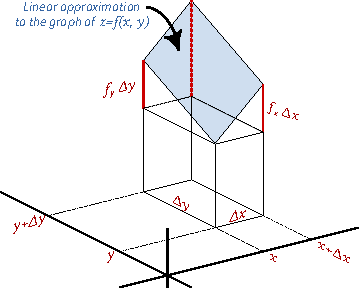
\includegraphics{01totaldifferential.pdf}
    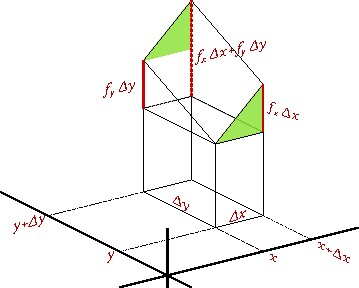
\includegraphics{01totaldifferential-no-tangentplane.pdf}
    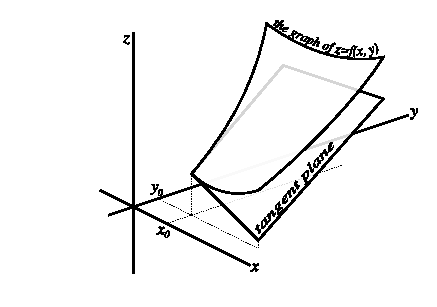
\includegraphics{01tangentplane.pdf}
  \end{center}
  \caption{\textbf{Top: } The graph of the linear approximation of $f$ (graph of
    $f$ itself is not shown -- see the bottom figure).  If we increase $x$ by
    $\Delta x$, then $f$ will increase by approximately $f_x \Delta x$, and if
    we increase $y$ by $\Delta y$, then $f$ increases by approximately $f_y
    \Delta y$.  If we increase $x$ and $y$ by $\Delta x$ and $\Delta y$ at the
    same time, then $f$ increases by roughly $f_x\Delta x+f_y \Delta y$. The
    vertical dotted line behind
    the parallelogram represents this increase in $f$.\\
    \null\quad\textbf{Bottom: } The graph of a function, and of its tangent
    plane at some point $(x_0, y_0, z_0)$. The tangent plane is the graph of the
    linear approximation to $f$. }
  \label{fig:total-differential-and-tangent-plane}
\end{figure}



\subsection{Example: tangent plane to the saddle surface at the origin}     
\textit{Find the equation for the tangent plane to the saddle surface $z=xy$ at
  the origin.  }

\textit{Solution: } The saddle surface is the graph of the function $f(x, y) =
xy$ whose partial derivatives are $f_x(x, y) = y$ and $f_y(x,y) = x$.  To find
the tangent plane at $x_0=0$, $y_0=0$, we compute the partial derivatives,
\[
f_x(x, y) = \pdd{xy}x = y, \text{ so at $(x_0,y_0) = (0,0)$ we have } f_x(0,0) =
0,
\]
and
\[
f_y(x, y) = \pdd{xy}y = x, \text{ so at $(x_0,y_0) = (0,0)$ we have } f_y(0,0) =
0,
\]
Moreover, we also have $f(x_0,y_0) = f(0,0) = 0$, so that the equation for the
tangent plane is
\[
z= 0 + 0\cdot(x-0) + 0\cdot(y-0) = 0,
\]
i.e.,
\[
z=0.
\]
The tangent plane at the origin is just the $xy$-plane.

\begin{figure}
  \centering
  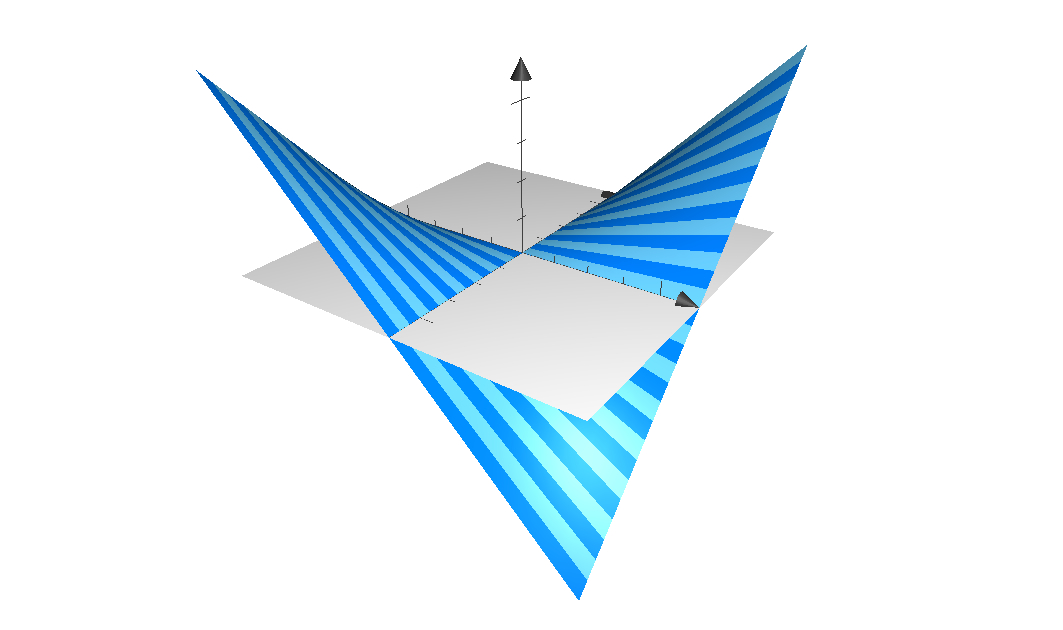
\includegraphics[width=0.7\textwidth]{02saddle-with-tangent.jpg}
  \caption{The graph of $z=xy$ and the tangent plane at the origin. }
  \label{fig:saddle-with-tangent}
\end{figure}

\subsection{Example: another tangent plane to the saddle surface}
\label{sec:another-tangent-to-the-saddle}%
\textit{Find the equation for the tangent plane to the saddle surface $z=xy$ at
  the point $(2,1,2)$.  Where does this plane intersect the coordinate axes?}

\textit{Solution: } This is almost the same problem as before.  The only
difference is that we are trying to find the tangent plane at a point other than
the origin.  To get the tangent plane at the point $(x_0,y_0) = (2,1)$ we
compute the derivatives
\[
f_x(x,y) = y \implies f_x(2,1) = 1,
\]
and
\[
f_y(x, y) = x \implies f_y(2,1) = 2.
\]
The equation for the tangent plane is therefore
\begin{align}
  \label{eq:tangent-to-saddle}
  z &= x_0y_0 + y_0(x-x_0) + x_0(y-y_0)\\
  &= 2+1\cdot(x-2)+2\cdot(y-1) \nonumber\\
  &= -2 +x +2y \nonumber
\end{align}
The intersections with the $x$, $y$ and $z$ axes are, respectively, $(2,0,0)$,
$(0,1,0)$, and $(0,0,-2)$.

\subsection{Example: tangent plane to a sphere}
\label{sec:tangent-plane-to-sphere-as-graph}%
\textit{The point $(x_0, y_0, z_0)$ lies on the upper half of the sphere with
  radius 4 centered at the origin.  Find an equation for the tangent plane to
  the sphere at that point, if $x_0 = 1$ and $y_0=3$.}

  \smallskip

\noindent%
\begin{minipage}{0.48\textwidth}
  \setlength\parindent{16pt}%
  \textit{\color{badgerred}Solution: } The equation for the sphere is
  $x^2+y^2+z^2 = 4^2 = 16$, so the upper half is the graph of the function
  \[
  f(x, y) = \sqrt{16 - x^2 - y^2}.
  \]
  The $z$ coordinate of the given point is therefore $z_0 = \sqrt{16-1^2-3^2} =
  \surd{6}$.  The partial derivatives of $f$ at $(x_0,y_0) = (1,3)$ are
  \begin{align*}
    \pdd fx&= \frac{-x_0}{\sqrt{16 - x_0^2 - y_0^2}} = -\frac{1}{\surd6}, \\
    \pdd fy&= \frac{-y_0}{\sqrt{16 - x_0^2 - y_0^2}} = -\frac{3}{\surd6}.
  \end{align*}
  The equation for the tangent plane is then
  \begin{align*}
    z &= \surd6 - \frac{1}{\surd6}(x-1) - \frac{3}{\surd6}(y-3)\\
    &=\frac{16}{\surd6} - \frac{x}{\surd6} - \frac{3y}{\surd6}.
  \end{align*}
\end{minipage}
\hfill
\begin{minipage}{0.48\textwidth}
  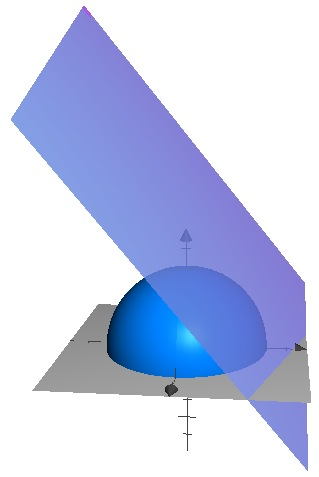
\includegraphics[width=0.8\textwidth]{02sphere-with-tangent.jpg}
\end{minipage}

\section{The Two Variable Chain Rule}
\subsection{The chain rule}
\label{sec:chain-rule-derivation}
Given two functions $x=x(t)$, $y=y(t)$ of one variable, and a function $z=f(x,
y)$ of two variables, then what is the derivative of the function
\[
g(t) = f(x(t), y(t))?
\]
We can find a general formula for $g'(t)$ by using the linear approximation
(\S~\ref{sec:the-linear-approximation-of-a-function}) in the following way.

To find $g'(t_0)$ for some $t_0$, we must compute
\[
\frac{g(t_0 + \Delta t) - g(t_0)}{\Delta t}
\]
and let $\Delta t\to 0$.

If $t$ increases by an amount $\Delta t$ from $t_0$ to $t_0+\Delta t$, then $x$
and $y$ will also change.  We write $\Delta x$ and $\Delta y$ for the changes in
$x$ and $y$, i.e.
\[
\Delta x = x(t_0+\Delta t) - x_0 , \qquad \Delta y = y(t_0+\Delta t) - y_0,
\]
where $x_0 = x(t_0)$ and $y_0=y(t_0)$.  The resulting change in $g$ is thus
\begin{align*}
  \Delta g &= g(t_0+\Delta t) - g(t_0)\\
  &= f\bigl( x(t_0+\Delta t), y(t_0+\Delta t)\bigr) - f\bigl(x(t_0), y(t_0)\bigr) \\
  &= f(x_0+\Delta x, y_0+\Delta y) - f(x_0, y_0).
\end{align*}
By the linear approximation formula \eqref{eq:linear-approximation-with-error}
one then has
\[
\frac{\Delta f}{\Delta t} = f_x(x_0, y_0) \frac{\Delta x}{\Delta t} + f_y(x_0,
y_0) \frac{\Delta y}{\Delta t} + e_x \frac{\Delta x}{\Delta t} + e_y
\frac{\Delta x}{\Delta t}
\]
As we let $\Delta t\to0$ the quotients $\Delta x/\Delta t$ and $\Delta y/\Delta
t$ converge to $x'(t_0)$ and $y'(t_0)$, while the errors $e_x$ and $e_y$
converge to zero, so we get \emph{the two-variable chain rule:}
\begin{equation}
  \label{eq:chain-rule-fxnotation}
  \frac{d f(x(t), y(t))}{dt}
  = f_x(x_0,y_0)\cdot x'(t_0) + f_y(x_0,y_0) \cdot y'(t_0).  
\end{equation}
The chain rule is often also written as
\begin{equation}\label{eq:chain-rule}
  \frac{df}{dt} = \pdd fx \frac{dx}{dt} 
  + \pdd fy  \frac{dy}{dt}.
\end{equation}
This form becomes easy to remember if we interpret the first term as ``the
change in $f$ caused by the change in $x$'' and the second term as ``the change
in $f$ caused by the change in $y$.''

In the way \eqref{eq:chain-rule} is written a number of details are swept under
the rug: the two derivatives $\frac{dx}{dt}$ and $\frac{dy}{dt}$ are ordinary
(Math 221) derivatives of the two functions $x(t)$ and $y(t)$; the two partial
derivatives $\frac{\pd f}{\pd x}$ and $\pdd fy $ are the partial derivatives of
$f$ \emph{in which one has substituted $x(t)$ and $y(t)$.}  A more correct way
of writing the equation would be
\begin{equation}
  \frac{df(x(t), y(t))}{dt}
  = \pdd fx (x(t), y(t)) \cdot x'(t) + \pdd fy (x(t), y(t)) \cdot y'(t).
  \label{eq:chain-rule-Leibniz-verbose}
\end{equation}
Many people find \eqref{eq:chain-rule} easier on the eyes, so that is what we
will usually write.

\subsection{The difference between $d$ and $\pd$}     
Compare \eqref{eq:chain-rule} with the linear approximation formula
\eqref{eq:linear-approximation-infinitesimal} with infinitesimal small
quantities.  Equation \eqref{eq:chain-rule} is just
\eqref{eq:linear-approximation-infinitesimal} in which one has divided both
sides by $dt$.  In contrast to equation
\eqref{eq:linear-approximation-infinitesimal} which contains the strange
``infinitely small quantities'' $dx$, $dy$, $df$, equation \eqref{eq:chain-rule}
contains the derivatives $\frac{dx}{dt}$, etc.\ which \emph{are} well-defined.

Note that we have a breakdown of Leibniz's notation: if we ignore the
distinction between ``$d$'' and ``$\pd$'', and just cancel $dx$ and $\pd x$, and
also $dy$ and $\pd y$ on the right then we end up with
\[
\frac{df}{dt} = \frac{\pd f} {\cancel{\pd x}} \frac{\cancel{dx}} {dt} +
\frac{\pd f} {\cancel{\pd y}} \frac{\cancel{dy}} {dt} = \frac{\pd f}{dt} +
\frac{\pd f}{dt} = 2\frac{\pd f}{dt},
\]
which doesn't make a lot of sense.  The moral: don't cancel $dx$ against $\pd
x$!


\subsection{An example} 
Suppose $x(t) = \cos\omega t$ and $y(t)=\sin \omega t$, so that $\vx(t)=
x(t)\ves1 + y(t)\ves2$ traces out the unit circle.
\begin{center}
  \itshape How fast does $S(t) = 2x(t) + 3y(t)$ change along this motion?
\end{center}
In other words, what can we say about $\frac{dS}{dt}$?

The quantity $S(t)$ is the composition of a function of two variables with the
functions $x(t)$ and $y(t)$, i.e.~it is the result of substituting $x(t)$ and
$y(t)$ in the function $f(x, y) = 2x+3y$.


\subsubsection*{Answer 1 -- without using the chain rule} We can simply compute
$S(t) = \cos\omega t + \sin \omega t$ and differentiate:
\begin{equation}
  \frac{dS}{dt} = \frac{d}{dt}\Bigl\{2\cos \omega t + 3\sin \omega t\Bigr\}
  = -2\omega\sin \omega t + 3\omega \cos\omega t.
  \label{eq:chainrule-example-answer1}
\end{equation}
Note that we did not use our new two-variable chain rule here.  This answer
shows that the point of the two-variable chain rule is not to compute
$\frac{d}{dt}f(x(t), y(t))$ in situations where we have formulas for the
functions $f(x,y)$, $x(t)$, and $y(t)$.  In such a situation we can always
substitute $x(t)$ and $y(t)$ in the function $f(x, y)$ after which we get a
function $S(t) = f(x(t), y(t))$ of one variable.  We learned how to
differentiate those in our first calculus course.

\subsubsection*{Answer 2 -- using the chain rule}
The quantity we want to differentiate is
\[
S(t) = f\bigl(x(t), y(t)\bigr),
\]
where
\[
f(x, y) = 2x+3y, \quad \text{and}\quad x(t) = \cos\omega t, \quad y(t) =
\sin\omega t.
\]
The chain rule tells us that
\begin{equation}
  \frac{dS}{dt} =
  \pdd fx \frac{dx}{dt}  + \pdd fy \frac{dy}{dt}.
  \label{eq:chainrule-example}
\end{equation}
Here the first term stands for the change in $S$ that is caused by the change in
$x$.  To compute it we first find
\[
\pdd fx = \pdd{\{2x+3y\}}x = 2,
\]
so that
\[
\pdd fx \frac{dx}{dt} = 2\cdot \frac{dx}{dt}.
\]
Similarly, the second term in \eqref{eq:chainrule-example} represents the change
in $S(t)$ due to the fact that $y$ is changing:
\[
\pdd fy = \pdd{\{2x+3y\}}y = 3 \implies \pdd fy \frac{dy}{dt} = 3\cdot
\frac{dy}{dt}.
\]
To get the rate of change of $S$ we add both the $x$ and $y$ contributions to
this rate of change, which leads us to
\begin{equation}
  \label{eq:chainrule-example-intermediate-result}
  \frac{dS}{dt} =  2\cdot \frac{dx}{dt} + 3\cdot \frac{dy}{dt}.
\end{equation}
So far we have not used what we know about $x(t)$ and $y(t)$.  This expression
we have just derived for $dS/dt$ is true no matter which $x(t)$, $y(t)$ we are
given.  In our case we have
\begin{align*}
  x(t) &= \cos \omega t \implies \frac{dx}{dt} = -\omega \sin \omega t,\\
  y(t) &= \sin \omega t \implies \frac{dy}{dt} = +\omega \cos \omega t.
\end{align*}
Substitute this in \eqref{eq:chainrule-example-intermediate-result}:
\[
\frac{dS}{dt} = -2\omega\sin \omega t + 3\cos \omega t,
\]
as before.

\subsubsection*{The moral:}
In this example the answer using the chain rule was longer, much more verbose,
and perhaps more complicated than the straightforward computation that led to
our first answer \eqref{eq:chainrule-example-answer1}.  Indeed, if the
derivative of $S$ is all we want then our first computation is the most
efficient way of getting $dS/dt$.  However, the computation using the chain rule
did give us some useful intermediate results, such as the general expression
\eqref{eq:chainrule-example-intermediate-result} for $dS/dt$.  This expression
remains valid if we change the path $(x(t), y(t))$ and can therefore be useful
in situations where, for example, we are allowed to choose the path and we would
like to choose a path for which $dS/dt$ has some prescribed value (e.g.~suppose
we want to keep $S$ constant, how do we choose the path?)

\subsection{Another example} 
Suppose the temperature at the point $(x,y)$ in the plane is given by $T(x, y)$,
and suppose that an ant is walking along the parametrized curve
\[
x(t) = R\cos \omega t, \quad y(t) = R\sin \omega t.
\]
Thus the ant is walking on a circle with radius $R$, and with angular velocity
$\omega$.
\begin{center}\itshape
  How fast is the temperature of the ant changing?\\
  i.e.~compute $\frac{dT}{dt}$.
\end{center}
Here we are not given an explicit formula for the function $T(x,y)$, so we
cannot substitute $x(t)$ and $y(t)$ in $T$ and differentiate using only our
first semester calculus skills.  The approach in Answer 1 of our previous
example does not apply here; we must use the chain rule.

\begin{figure}[h]
  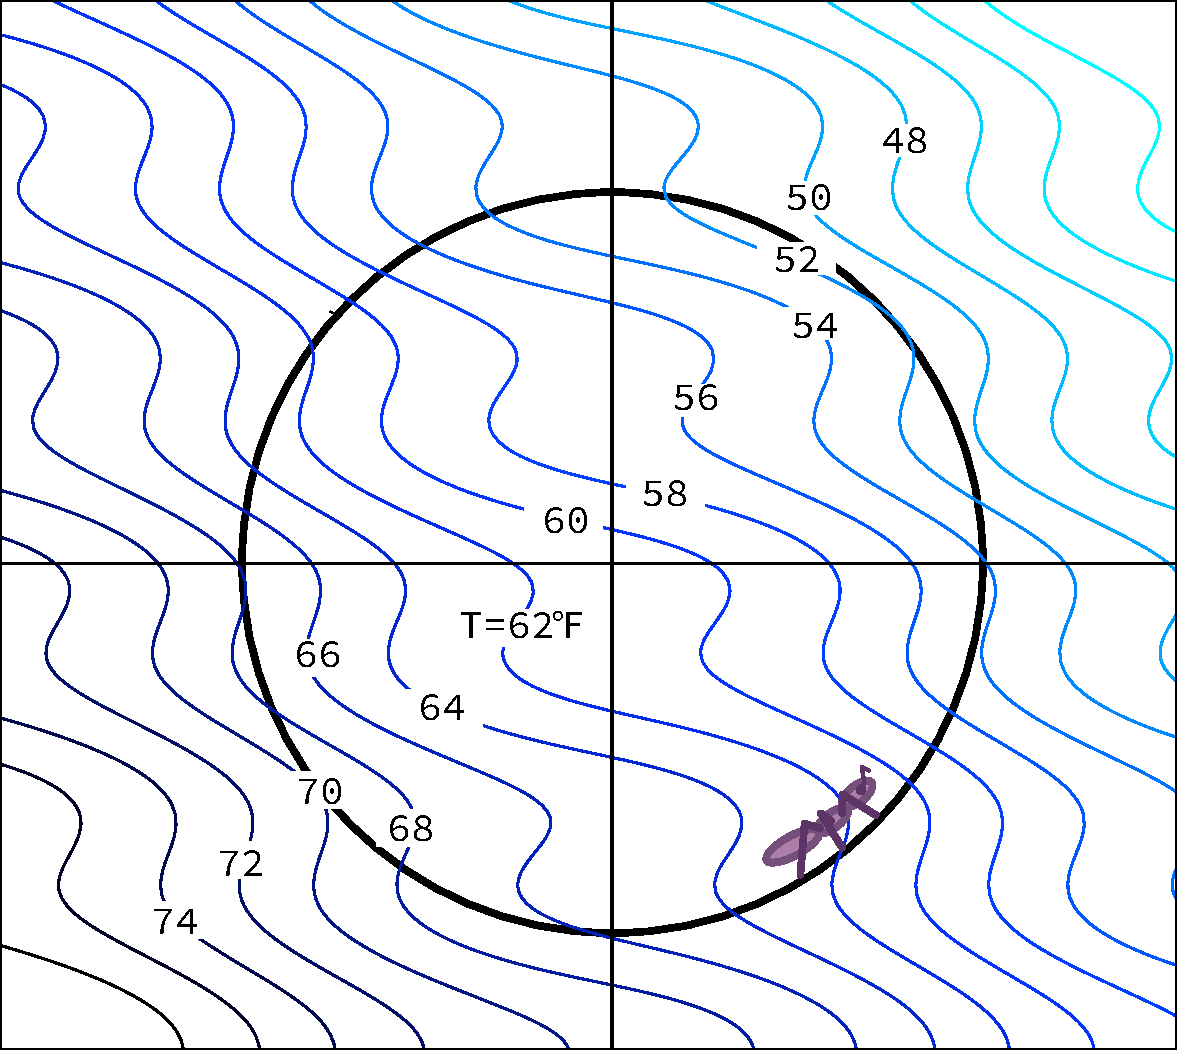
\includegraphics[width=0.5\textwidth]{temperature-of-ant.pdf}
  \caption{Ant walking in a region of varying temperature.}
  \label{fig:temperature-of-ant}
\end{figure}
In \S~\ref{sec:chain-rule-derivation} we have seen several equivalent ways of
writing the chain rule.  Let us look at two of these and consider the meaning of
the terms that arise.

The short form \eqref{eq:chain-rule} of the chain rule tells us that
\[
\frac{dT}{dt} = \pdd Tx \frac{dx}{dt} + \pdd Ty \frac{dy}{dt}.
\]
The $T$ on the left stands for $T(x(t), y(t))$, which we can interpret as the
temperature at the point $(x(t), y(t))$.  That point is the location of the ant
at time $t$, so the $T$ on the left is the temperature the ant feels at time
$t$.  This is a function of $t$.  In mathematical terms it is the result of
substituting (composing) the functions $x(t)$ and $y(t)$ in the function
$T=T(x,y)$.

The two $T$'s on the right appear in partial derivatives.  Here $\pdd Tx$ stands
for the partial derivative of the function $T=T(x, y)$ with respect to the
variable $x$.  One can compute this without knowing the ant's path $(x(t),
y(t))$.  Similarly, $\pdd Ty$ is the partial derivative of $T$ with respect to
$y$.  The partial derivatives $\pdd Tx$ and $\pdd Ty$ themselves are again
functions of $x$ and $y$.  \textit{After} computing these partials they are
meant to be evaluated at the point $(x(t), y(t))$.

This leads us to the more verbose version \eqref{eq:chain-rule-Leibniz-verbose}
of the chain rule, which tells us
\[
\frac{dT(x(t), y(t))}{dt} = \pdd Tx(x(t), y(t))\cdot x'(t) + \pdd Ty(x(t),
y(t))\cdot y'(t).
\]
At this point the only additional information we have is about the ant's motion,
namely, $x(t) = R\cos\omega t$ and $y(t) = \sin \omega t$.  We can compute the
derivatives of $x(t)$ and $y(t)$, which gives us the velocity of the ant in the
$x$ and $y$ directions:
\[
x'(t) = -\omega R\sin \omega t, \qquad y'(t) = \omega R\cos\omega t.
\]
If we substitute everything we know in the chain rule we find that the rate at
which the ant's temperature changes is
\[
\frac{dT}{dt} = -\pdd Tx(R\cos \omega t, R\sin\omega t)\cdot \omega R\sin \omega
t + \pdd Ty(R\cos \omega t, R\sin\omega t)\cdot \omega R \cos\omega t.
\]
To make the equation more readable one can leave out the $(R\cos \omega t,
R\sin\omega t)$, which results in
\[
\frac{dT}{dt} = -\omega R\sin \omega t\pdd Tx + \omega R \cos\omega t\pdd Ty .
\]
The disadvantage of this shorter version is that the reader has to figure out
where we intended to evaluate the two partial derivatives $\pdd Tx$ and $\pdd
Ty$.

\section{Problems}
\begin{multicols}{2}\problemfont

\problem Find the linear approximation to $f(x, y)$ at the point 
$(a,b)$ in the following cases:

\subprob $f(x, y) = xy^2$, $(a, b) = (3,1)$.
\answer
The linear approximation formula is equation
\eqref{eq:linear-approximation-no-error}, in which $x_0 = a = 3$,
$y_0 = b= 1$, and $\Delta x = x-a = x-3$, $\Delta y = y-b = y-1$.  So
for this problem the linear approximation of $f(x,y) = xy^2$ at
$(3,1)$ is
\[
f(x, y) \approx 3 + (x-3) + 6 (y-1) = x+6y-6.
\]
This approximation is only expected to be good when $(x,y)$ is close
to $(3,1)$.  The approximation contains an error which is small
compared to $|x-3|$ and $|y-1|$. 

\noindent
\textbf{FAQ:} What is the relation between the linear approximation
and the tangent plane?

\noindent\textit{Answer:} They are very closely related: the tangent
plane is the graph of the linear approximation. The linear
approximation is the equation for the tangent plane.  To compute
either you have to do the same thing.

\endanswer

\subprob $f(x, y) = x/y^2$, $(a, b) = (3,1)$.
\answer
$x/y^2 \approx 3 + (x-3) - 6 (y-1) = x-6y+6$ when $x$ is close to $3$
and $y$ is close to $1$.
\endanswer

\subprob $f(x, y) = \sin x+ \cos y$, $(a, b) = (\pi,\pi)$.
\answer
$\sin x + \cos y \approx -1 + (-1)(x-\pi) + (0)(y-\pi) = \pi-1-x$ when
$x$ is close to $\pi$ and $y$ is close to $\pi$.
\endanswer


\subprob $f(x, y) = xy/(x+y)$, $(a, b) = (3,1)$.
\answer
$\frac{xy}{x+y} \approx \frac34 + \frac{1}{16}(x-3) + \frac 9 {16}(y-1)$
 when $x$ is close to $3$ and $y$ is close to $1$.
\endanswer

\problem Find an equation for the plane tangent to the graph of $\DS 
f(x,y)=\sin(xy)$ at $(\pi,1/2,1)$. 
\answer
$z=1$
\endanswer

\problem Find an equation for the plane tangent to the graph of $\DS 
f(x,y)=x^2+y^3$ at $(3,1,10)$. 
\answer
$z=6(x-3)+3(y-1)+10$
\endanswer

\problem Find an equation for the plane tangent to the graph of $\DS 
f(x,y)=x\ln(xy)$ at $(2,1/2,0)$. 
\label{prb:ln-tan-plane}
\answer
$z=(x-2)+4(y-1/2)$
\endanswer

% \problem \subprob Find an equation for the tangent plane to the graph of $f(x,
% y) = x^2-2xy$ at the point with $x=2$, $y=1$.

% Find the intersection of the graph of $f$ and the tangent plane you found.
% Show that it consists of two lines.  (Hint: compare with the example in
% \S\ref{sec:01intersect-tangent-with-graph}).  \answer
% % REWRITE THIS
% The graph has equation $z=x^2-2xy$, The tangent plane has equation $z=2x-4y$.

% The part of the tangent plane which lies under the graph is given by
% \[
% 2x-4y < x^2-2xy,
% \]
% i.e.\ by
% \[
% x^2-2xy-2x+4y >0
% \]
% With some luck you see that the LHS can be factored as
% \[
% x^2-2xy-2x+4y = (x-2)(x-2y),
% \]
% so that the part of the tangent plane which is under the graph consists of
% those points $(x,y)$ for which either
% \[
% x>2, \text{ and } x>2y
% \]
% or
% \[
% x<2, \text{ and } x<2y
% \]
% holds.

% The tangent plane and graph intersect along the lines $x=2$ and $x=2y$.
% \begin{center}
%   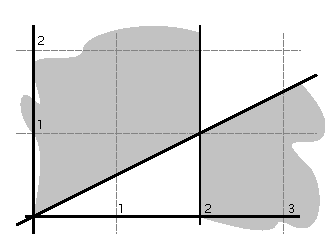
\includegraphics{tangent-below-quadric.pdf}
% \end{center}

% \endanswer

\problem\subprob\label{prb:not-implicit-yet}
Find an equation for the plane tangent to the surface defined by $\DS
2x^2+3y^2-z^2=4$ at $(1,1,-1)$.  (Hint: first write the surface as a graph
$z=f(x, y)$).
\answer
Solve for $z$: $z=\pm\sqrt{2x^2+3y^2-4}$.  In this problem we are
looking at the point $(1,1,-1)$ so we have the graph of $z=f(x,y) = -
\sqrt{2x^2+3y^2-4}$.  The partials are 
\[
\pdd fx = \frac{-2x}{\sqrt{2x^2+3y^2-4}},\qquad
\pdd fy = \frac{-3y}{\sqrt{2x^2+3y^2-4}}
\]
so that, at $(1,1,-1)$ you get $f_x = -2$, $f_y = -3$.  There for the
equation for the tangent plane is $z=-2(x-1)-3(y-1)-1$
\endanswer

\subprob The same question at the point $(1,1,+1)$.


\problem \subprob Suppose you have computed the two partial 
derivatives of a function $z=f(x_0, y_0)$, and you found $f_x(x_0, y_0) = A$ and
$f_y(x_0, y_0) = B$.  Find a normal vector to the tangent plane of the graph of
$z=f(x, y)$ at $(x_0, y_0, z_0)$.

(Hint: If you know the equation for a plane, then how do you find a normal
vector to this plane?)
\answer
The tangent plane has equation $z= z_0 + A(x-x_0) + B(y-y_0)$.  By
putting the variables $x,y,z$ on one side, and all the constants on
the other, you can write this as
\[
Ax +By - z = Ax_0+By_0-z_0.
\]
This is the equation for a plane whose normal is $\vn = \tvek
A\\B\\-1\ttor$.  Any other multiple of this vector is also a valid
normal to the plane, in particular, $\tvek -A\\-B\\+1\ttor$ is OK.

\endanswer

\subprob Find an equation in vector form for the tangent plane to $\DS
x^2+4y^2=2z$ at $(2,1,4)$.  Also find an equation for the normal line to the
graph at $(2,1,4)$.  (The normal line to the graph of a function at some
point $P$, is the line through $P$ that is perpendicular to the
tangent plane to the graph at $P$.)
\answer
We want a normal to the graph of $z = f(x, y) = \frac{1}{2}x^2 + 2y^2$ at the
point $P$.  By the previous problem a normal is given by $\vn = \tvek f_x(2,1)
\\ f_y(2,1) \\ -1 \ttor = \tvek 2\\4\\-1\ttor$.

A line through $P$ in the direction of $\vn$ is given by $\vr (t)=\tvek
2\\1\\4\ttor+t\tvek 2\\4\\-1\ttor$
\endanswer



\problem Imagine a differentiable function, $f(x,y)$.  Make a good 
drawing of the function $f$ and show how $f_x(a, b)$ and
$f_y(a,b)$ are the slopes of two lines which are tangent to the graph
at $(a,b)$.  Indicate clearly which two lines you mean, and describe
how they are defined.

(Can't think of a nice graph?  Take something like the bottom drawing
in Figure~\ref{fig:total-differential-and-tangent-plane}.)
\answer
Below you see the graph of a function and two (solid) lines
which are tangent to the graph.  On one line you have $x=a$
(hence constant), and its slope is $f_x(a,b)$; on the other you have
$y=b$, and it has slope $f_y(a,b)$. 
\begin{center}
  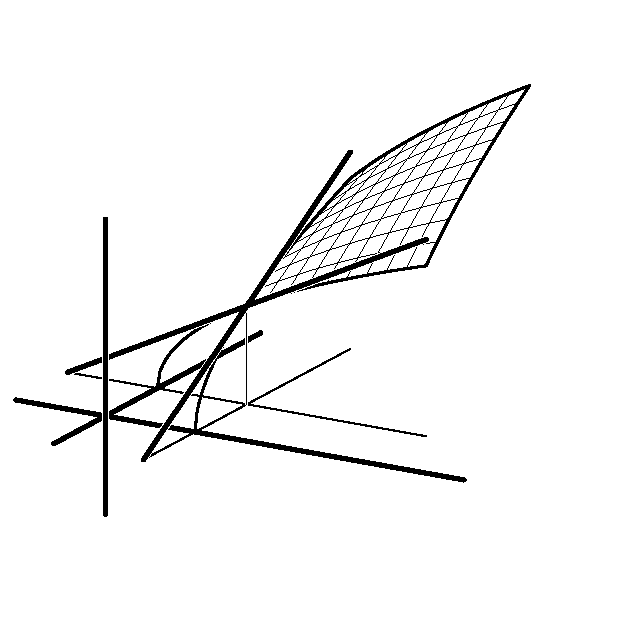
\includegraphics{03two-tangents.pdf}
\end{center}
The tangent plane to the graph (not drawn here, but see
Figure~\ref{fig:total-differential-and-tangent-plane} in the notes)
is the plane containing the two lines in the drawing.
\endanswer

\problem Let $f$ be as in problem~\ref{prb:ln-tan-plane}.  Use linear 
approximation to approximate $f(1.98, 0.4)$ by hand.  Compare your
answer with the actual value of $f(1.98, 0.4)$ (you'll need a
calculator).
\answer
The function is $f(x, y) = x \ln(xy)$.
We have $f(2, \frac{1}{2}) = 2\ln(2\cdot \frac12) = \ln 1 = 0$.
The gradient of the function is $\nab f = \tvek \ln(xy) + 1  \\
x/y\ttor$.
At the point $(2, \frac{1}{2})$ this is $\nab f = \tvek 1 \\ 4\ttor$,
so the linear approximation is 
\[
f(x, y) \approx f(2, \frac{1}{2}) + 1\cdot(x-2)+4\cdot(y-\frac12),
\]
i.e.
\[
f(x, y) \approx 1(x-2) + 4(y-\frac12).
\]
(This is also the answer to problem~\ref{prb:ln-tan-plane}.)

Here we don't want to describe the tangent plan, but we want to find
the value of $f(x, y)$ for $(x,y) = (1.98, 0.4)$.  Substituting these
values of $x$ and $y$ in the linear approximation we get $f(1.98, 0.4)
\approx (1.98-2) + 4 (0.4-0.5) = -0.42$.

This is only an approximation, and you wonder how good it is.  We have
$\Delta x = 1.98-2 = -0.02$, and $\Delta y = 0.4 - \frac12 =
-0.1$\ldots are these numbers ``small''?  To find the error in the
approximation you could use a Lagrange-type remainder term, but that's
not part of math 234.  Instead we grab a calculator and compute
$f(1.98, 0.4) = 1.98\cdot \ln(1.98\cdot 0.4) = -0.46172\cdots$.  So
our linear approximation formula is off by $0.04\cdots$.

\endanswer
\problem
\subprob The tangent plane to the saddle surface $z=xy$ at the origin intersects
the graph of the saddle surface in two lines.  Which lines are they?
\answer
The $x$-and $y$-axes.
\endanswer

\subprob Consider the tangent plane to the saddle surface at $x=2, y=1$
that was computed in \S\ref{sec:another-tangent-to-the-saddle}.  Let $(x,y,z)$
be a point on the saddle surface, and let $(x,y,z_*)$ be the point on the
tangent plane with the same $x$ and $y$ coordinates.  What is the
difference in heights of these two points?
\answer
The heights are the $z$-coordinates, so $z=xy$ and $z_* = -2+x+2y$.  The
difference is
\[
z-z_* = xy - (-2+x+2y) = xy-x-2y+2.
\]
\endanswer

\subprob Show that the saddle surface and its tangent plane intersect when $x=2$
or $y=1$.

\problem
\subprob Find an equation for the tangent) plane to the graph of
$f(x, y) = xy$ at the point $(a, b, ab)$.  Here $a$ and $b$ are
constants which will appear in your answer.
\answer The tangent plane has equation $z=
ab +b(x-a) + a(y-b) = bx+ay-ab$.
\endanswer

\subprob Show that the intersection of the tangent plane and the graph
consists of two straight lines.
\answer The point $(x, y, z)$ lies on the intersection if $z=xy$ and
$z=bx+ay-ab$.  Therefore $x$ and $y$ must satisfy 
$xy-bx-ay+ab = 0$.  This equation factors as follows:
\[
xy-bx-ay+ab = (x-a)(y-b) =0,
\]
so that the intersection contains the line $x=a$, $z=ay$, and
also the line $y=b$, $z=bx$.
\endanswer



\end{multicols}


\section{Gradients}

\subsection{The gradient vector of a function}     
The right hand side in the chain rule \eqref{eq:chain-rule-fxnotation} can be
written as a dot-product of two vectors, namely
\begin{align}
  \label{eq:chainrule-as-dotprod}
  \frac{df}{dt}
  &= f_x(x_0,y_0)\cdot x'(t_0) + f_y(x_0,y_0)\cdot y'(t_0)\\
  &= \vek f_x(x_0, y_0) \\ f_y(x_0, y_0)\tor \dpp \vek x'(t_0) \\
  y'(t_0)\tor\nonumber
\end{align}
This turns out to be so useful that the vector containing the derivatives of $f$
has been given a name.  It is called the \emph{gradient of $f$}, and it is
written as
\begin{equation}
  \nab f(x, y) \stackrel{\sf def}= \vek f_x(x, y) \\ f_y(x, y) \tor
  \label{eq:gradient-defined}
\end{equation}
The symbol $\nab$ is pronounced ``nabla.''

The chain rule, written in vector form, looks like this:
\begin{equation}
  \frac{d f(\vx(t))}{dt} = \nab f(x(t)) \,\dpp\, \vx'(t)
  \label{eq:chainr-rule-vector-form}
\end{equation}
The linear approximation formula \eqref{eq:linear-approximation-no-error} can
also be rewritten more compactly using the gradient vector:
\begin{equation}
  f(\vx_0+\Delta\vx) \approx f(\vx_0) +  \nab f(\vx_0)\,\dpp\, \Delta\vx.
  \label{eq:linear-approximation-vectorform}
\end{equation}
\subsection{The gradient as the ``direction of greatest increase'' for a
  function $f$}
\label{sec:01grad-is-direction-of-greatest-increase}
When we apply the formula
\begin{equation}\label{eq:recall-dot-product}
  \va\dpp\vb = \|\va\|\; \|\vb\|\cos\angle(\va,\vb)
\end{equation}
for the dot product to the vector form
\eqref{eq:linear-approximation-vectorform} of the linear approximation equation,
we find a very useful interpretation of the gradient.  If we are at a point with
position vector $\vx_0$ ($P$ in figure \ref{fig:steepestincrease}) and we are
allowed to make a small step $\Delta \vx$ in any direction we like, but of
prescribed length, then which way should we go if we want to increase $f$ as
much as possible?  And where should we go if, instead, we want to decrease $f$
as much as possible?  What if we want to keep $f$ the same?

\begin{figure}[t]
  \centering \begin{picture} (240.000000,161.967213)(0,0)
    \put(0.0, 0.0){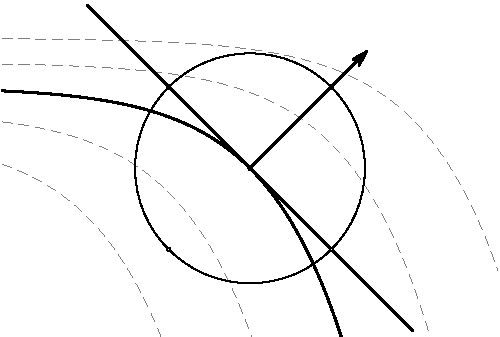
\includegraphics{01steepestdescent.pdf}}
        \put(177.18, 138.16){\sffamily\itshape \makebox[0pt][l]{$\nab f(P)$}}
    \put( -1.05, 117.06){\sffamily\itshape \makebox[0pt][r]{f = 0.0}}
    \put( -1.05,  81.24){\sffamily\itshape \makebox[0pt][r]{-0.6}}
    \put( -1.05, 102.01){\sffamily\itshape \makebox[0pt][r]{-0.3}}
    \put( -1.05, 129.99){\sffamily\itshape \makebox[0pt][r]{0.3}}
    \put( -1.05, 142.15){\sffamily\itshape \makebox[0pt][r]{0.6}}
    \put(154.02, 117.00){\sffamily\itshape \makebox[0pt][r]{$A$}}
    \put( 77.98, 117.00){\sffamily\itshape \makebox[0pt][r]{$B$}}
    \put(159.02,  31.97){\sffamily\itshape \makebox[0pt][c]{$C$}}
    \put( 79.98,  33.97){\sffamily\itshape \makebox[0pt][r]{$D$}}
    \put(117.00,  70.98){\sffamily\itshape \makebox[0pt][r]{$P$}}

\end{picture}

  \caption{The gradient as direction of fastest increase: if we are at a point
    $P$, and we are allowed to jump to any point at a given fixed distance from
    $P$, and if we only know $\nab f(P)$, then the
    linear approximation formula tells us that\\
    \null\quad to maximize $f$ we follow the gradient (choose $A$); \\
    \null\quad to minimize $f$ we go in the direction opposite to
    $\nab f(P)$ (choose $D$); \\
    \null\quad to keep $f$ fixed we move perpendicular to the gradient (choose
    $B$ or $C$).}
  \label{fig:steepestincrease}
\end{figure}

From \eqref{eq:linear-approximation-vectorform} we see that the change in $f$ is
(approximately) given by
\[
\Delta f \stackrel{\rm def}{=} f(\vx +\Delta \vx) - f(\vx)
\stackrel{\textrm{\eqref{eq:linear-approximation-vectorform} } }{\approx} \nab f
\dpp \Delta \vx \stackrel{\text{\eqref{eq:recall-dot-product} }}{=} \|\nab f\|\;
\|\Delta \vx\| \; \cos \theta
\]
where $\theta$ is the angle between the gradient $\nab f$ and the vector $\Delta
\vx$ which represents the step we take.  In this formula the lengths $\nab f$
and $\|\Delta\vx\|$ are fixed, and the angle $\theta$ is the only thing we can
change.  Therefore the largest change in $f$ results if $\cos \theta=+1$, the
smallest when $\cos \theta=-1$, and no change will result if $\cos\theta=0$.  So
we conclude
\begin{itemize}
\item To increase $f$ as much as possible choose $\Delta\vx$ in the direction of
  the gradient $\nab f$,
\item To decrease $f$ as much as possible choose $\Delta\vx$ in the direction
  opposite to the gradient $\nab f$, i.e.\ in the direction of $-\nab f$,
\item To keep $f$ constant choose $\Delta\vx$ perpendicular to the gradient.
\end{itemize}
This is sometimes summarized by saying that \emph{the gradient $\nab f$ points
  in the direction of fastest increase for the function $f$.}

% \begin{equation}
%  \left.\frac{df(\vx + t\vv)}{dt}\right|_{t=0}
%  = \vv\dpp\nab f(\vx)
%  \label{eq:grad-times-vector}
%\end{equation}

%The gradient $\nab f(\vx)$ gives you the direction in which the function $f$
% increases the fastest, since
% \[
% \left.\frac{df(\vx + t\vv)}{dt}\right|_{t=0} = \vv\dpp\nab f(\vx) =
% \bigl\|\nab f(\vx)\bigr\| \, \|\vv\| \,\cos \theta
% \]
% where $\theta$ is the angle between the velocity $\vv$ and the gradient $\nab
% f(\vx)$.

\subsection{The gradient is perpendicular to the level curve}
\label{sec:01gradientperp2levelcurve}
Suppose that for some function $z=f(x,y) $ the level set at level $C$ is a
curve, and suppose that we have a parametric representation $\vx(t) = \tvek
x(t)\\y(t)\ttor$ of this curve.  This means that $x(t)$ and $y(t)$ satisfy
\[
f(x(t), y(t)) = C.
\]
By the chain rule we then get
\[
0= \frac{d f(\vx(t))}{dt} = \nab f(\vx(t)) \dpp \vx'(t),
\]
which tells us that the tangent vector $\vx'(t)$ to the level set is
perpendicular to the gradient $\nab f(\vx(t))$ of the function.  Therefore,
\begin{quote}
  \itshape if $\nab f(x_0,y_0)\neq\vvv0$, then $\nab f(x_0, y_0)$ is a normal
  vector to the tangent to the level curve of $f$ at $(x_0,y_0)$.
\end{quote}
We now have the necessary ingredients to write the equation for the tangent,
namely we know a point $(x_0,y_0)$ on the line, and we know a normal vector to
the line (the gradient).  Thus the equation for the tangent is
\[
\nab f (\vx_0) \dpp (\vx-\vx_0) = 0,
\]
or, equivalently,
\[
\pdd fx(x_0, y_0) \cdot (x-x_0) + \pdd fy(x_0, y_0) \cdot (y-y_0) = 0.
\]
\subsection{The tangent to the parabola $y=x^2$, again}
The very first example anyone sees in their first calculus course must surely be
the computation of the tangent to the parabola $y=x^2$ at the point $(x,y) =
(1,1)$.  We know the answer: it is a line with slope $2$, through the point
$(1,1)$.

We can interpret the parabola as the zero set of the function of two variables
given by $f(x, y) = y-x^2$, and therefore we should be able to find the same
tangent at $(1,1)$ by computing the gradient of $f$.  The computation goes like
this:
\[
f(x,y)=y-x^2 \implies \nab f(x, y) = \vek f_x\\f_y\tor = \vek -2x \\ y\tor.
\]
At $(x,y)= (1,1)$ we have
\[
\nab f(1,1) = \vek -2\\1\tor.
\]%
\marginpar{\centering%
  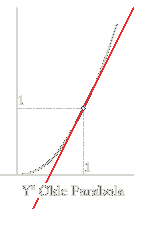
\includegraphics[scale=1.2]{YeOldeparabola.pdf}}%
This vector is perpendicular to the tangent to its zero set.  If we let
$\vx_0=\tvek1\\1\ttor$ be the position vector of our point on the parabola, then
the equation for the tangent to the parabola at this point is
\[
\vn\dpp(\vx-\vx_0) = 0,
\]
i.e.
\[
\vek -2\\1\tor\dpp \vek x-1 \\y-1 \tor = 0.
\]
Simplifying this we get
\[
-2\cdot(x-1) + 1\cdot(y-1)=0, \text{ and thus } y=2x-1.
\]
This is the same line that we found in our first calculus course.

\subsection{Example: the tangent to the zero set of $x^2-y^2+y^3$} 
Consider the zero set of the function
\[
f(x,y) = x^2-y^2+y^3.
\]
The resulting curve is not as familiar as the parabola from the previous
example, and drawing the curve takes some effort\footnote{One could start by
  solving the equation for $x$, which leads to $x=\pm y\sqrt{1-y}$.  This shows
  that $y\leq1$ on the curve.  Graphing $x=y\sqrt{1-y}$ using our 1st semester
  calculus skills then gives us half the curve; the other half is given by its
  reflection in the $y$-axis, i.e.~$x= -y\sqrt{1-y}$. }.

We will not try to draw the whole zero set in this example, but instead we will
see what happens when we try to find the tangent to the zero set at two
different points on the zero set, namely, at $(0,1)$ and at the origin.

\subsubsection*{The tangent at $(0,1)$}
To find the tangent at any point on the zero set of $f$ we use that the normal
to the tangent is given by the gradient of $f$
\[
\nab f = \vek f_x\\f_y\tor =\vek 2x \\ -2y+3y^2\tor.
\]
The normal to the tangent at the point $(0,1)$ is therefore
\[
\vn = \nab f(0,1) = \vek0 \\ -2+3\tor = \vek 0\\1\tor.
\]
In other words, the normal to the tangent at $(0,1)$ is the vertical unit vector
$\ves2$, and therefore the tangent is a horizontal line through $(0,1)$.  Its
equation is $y=1$.  We could also find this equation by working out the general
equation $\vn\dpp(\vx-\vx_0)=0$ for a line with a given normal and point.  Here
we have
\[
\vn = \nab f(0,1) = \vek0\\1\tor, \quad\vx_0 = \vek 0 \\1\tor,
\]
so the equation for the tangent is
\[
\vek0\\1\tor\dpp \vek x-0 \\ y-1\tor = 0,
\]
which simplifies to
\[
y-1=0.
\]

\subsubsection*{The tangent at the origin}
When we repeat the previous calculation at $(x_0, y_0) = (0,0)$ we run into
problems.  These problems begin when we compute the gradient $\nab f$ at the
origin:
\[
\nab f(0,0) = \vek2x \\-2y+3y^2\tor_{x=0, y=0} =\vek 0 \\ 0 \tor.
\]
The gradient at the origin turns out to be the zero vector.  This is problematic
because the zero vector has no direction, and thus is not perpendicular to any
particular line.  \textit{We cannot find the tangent at the origin!}

To see what is going on one has to take a closer look at the curve near the
origin -- see figure~\ref{fig:gradientANDlevels}.  It turns out that near the
origin the zero set of $f$ consists of two smooth curves that cross each
other.\footnote{One way to see this is to solve $x^2-y^2+y^3=0$ for $x$, which
  gives $x=\pm y\sqrt{1-y}$.  Near the origin $y$ is very small, so we can
  approximate $\sqrt{1-y} \approx \sqrt{1}=1$.  The zero set near the origin is
  therefore approximately described by $x=\pm y$, i.e.~two crossing lines.}  The
gradient has to be perpendicular to both of these curves, and the only vector
that achieves this is the zero vector.  Note also that there is no single line
that is tangent to the zero set at the origin.  If we had seen the drawing ahead
of time then we would not have expected to find a tangent to the zero set of $f$
at the origin.

\begin{figure}[ht]
  \begin{center}
    \input ../figures/234/01gradientANDlevels
  \end{center}
  \caption{The zero set of the function $f(x,y) = x^2-y^2+y^3$, and its gradient
    at various points on this zero set.  Since the gradient is always
    perpendicular to the level set of a function, a drawing of the zero set
    tells us the direction of the gradient.  However, the drawing does not say
    anything about the length of the gradient.}
  \label{fig:gradientANDlevels}
\end{figure}


\section{The chain rule and the gradient of a function of three variables}
\subsection{The gradient, etc.}
So far we have only looked at the gradient of a function of two variables.  But
for a function of three variables there is a very similar definition, and the
facts we have discovered have nearly identical counterparts.

If $u=f(x, y, z)$ is a function of three variables, then its gradient is defined
to be the vector
\[
\nab f(x,y,z) = \vek f_x(x, y, z) \\f_y(x, y, z) \\f_z(x, y, z) \tor.
\]
The \emph{chain rule} in this context says that, if $x=x(t)$, $y=y(t)$, and
$z=z(t)$ are functions of one variable, then the derivative of the function we
get by substituting $x(t), y(t), z(t)$ in $f$ is given by any of the following
three equivalent formulas
\begin{align}
  \label{eq:chainrule-threevariables}
  \frac{d f(x(t), y(t), z(t))}{dt}
  &= f_x(x(t), y(t), z(t))\,x'(t) + f_y(x(t), y(t), z(t))\,y'(t)\\
  &\hspace{8em} + f_z(x(t), y(t), z(t))\,z'(t) \nonumber \\[1ex]
  &= \pdd fx \frac{dx}{dt} + \pdd fy \frac{dy}{dt} + \pdd fz \frac{dz}{dt}
  \nonumber\\
  &= \nab f(\vx(t)) \dpp \vx'(t), \text{ where } \vx(t) = \vek
  x(t)\\y(t)\\z(t)\tor.  \nonumber
\end{align}
The linear approximation formula for the function $f$ at some point $(x_0, y_0,
z_0)$, which gives us an approximation of the amount by which $f$ increases if
we go from $(x_0, y_0, z_0)$ to $(x, y, z) = (x_0+\Delta x, y_0 + \Delta y, z_0+
\Delta z)$, is as follows:
\begin{align}
  \label{eq:linearapprox-threevariables}
  \Delta f &=
  f(x, y, z) - f(x_0, y_0, z_0)\\
  &\approx \pdd fx \cdot \Delta x + \pdd fy \cdot \Delta y + \pdd fz \cdot
  \Delta z, \nonumber
\end{align}
in which the partial derivatives are to be evaluated at $(x_0, y_0, z_0)$.
Compare this with the two variable version
\eqref{eq:linear-approximation-no-error-Deltaf}.  In vector form we have
\begin{multline}
  \Delta f = f(\vx_0 + \Delta\vx) - f(\vx_0)
  \approx \nab f(\vx_0) \dpp \Delta\vx,\\
  \text{ where } \vx_0 = \vek x_0\\y_0\\z_0\tor,\; \Delta \vx = \vek \Delta x\\
  \Delta y\\ \Delta x\tor.
  \label{eq:linearapprox-threevariables-vectorform}
\end{multline}
This is the same formula as in the two-variable case, where we had
\eqref{eq:linear-approximation-vectorform}.  The discussion about ``direction of
fastest increase'' applies to the three variable case without change.  Thus, if
we are at a point $\vx_0$, and we are allowed to change our position by a small
vector $\Delta\vx$ of a prescribed length, then we should choose $\Delta\vx$ in
the direction of the gradient $\nab f(\vx)$ if we want to increase $f$ as much
as possible; we should choose $\Delta\vx$ in the direction of $-\nab f(\vx)$ if
we want to \textit{decrease} $f$ as much as possible; and we should choose
$\Delta\vx$ perpendicular to $\nab f(\vx)$ if we want to keep $f$ constant.

\subsection{Tangent plane to a level set}       
If $t=f(x, y, z)$ is a function of three variables then it is hard to visualize
its graph, since this involves drawing \textit{four} mutually perpendicular
axes, something we, three dimensional creatures, cannot do.  However, we can try
to visualize the level sets of the function.  The level set at level $C$
consists, by definition, of all points in three dimensional space whose
coordinates satisfy the equation $f(x, y, z) = C$.

For instance, the unit sphere is given by the equation $x^2+y^2+z^2 = 1$, so it
is the level set at level $1$ of the function $f(x, y, z) = x^2+y^2+z^2$.  The
sphere with radius $R$ is the level set of the same function $f$ at level $R^2$.

Consider a function of three variables, and let $(x_0, y_0, z_0)$ be some point
on the level set at level $C$ (thus $f(x_0, y_0, z_0)=C$.)  The equation for the
level set itself is $f(x,y,z) = C$, and since $(x_0,y_0,z_0)$ satisfies this
equation we can write the equation for the level set as
\[
f(x,y,z) - f(x_0,y_0,z_0) = 0.
\]
Near the point $(x_0,y_0,z_0)$ we can use the linear approximation of $f$ to
approximate the equation for the level set of $f$.  We have
\[
f(x, y, z) - f(x_0, y_0, z_0) \approx \pdd fx \cdot (x-x_0) + \pdd fy \cdot
(y-y_0) + \pdd fz \cdot (z-z_0),
\]
where, as in \eqref{eq:linearapprox-threevariables}, the partial derivatives are
to be computed at the given point $(x_0, y_0, z_0)$.  They are, in particular,
constants (they depend on $(x_0, y_0, z_0)$ but not on $(x, y, z)$.)

\begin{figure}[h]
  \input ../figures/234/tangent-plane-to-levelset.pdf_tex
\end{figure}

Thus we see that near any particular point on the level set of a function we can
approximate the equation for the level set by
\begin{equation}
  \pdd fx \cdot (x-x_0) +
  \pdd fy \cdot (y-y_0) +
  \pdd fz \cdot (z-z_0) = 0.
  \label{eq:levelset-threevars}
\end{equation}
If at least one of the partial derivatives at $(x_0, y_0, z_0)$ is non zero,
then this is the equation of a plane. We call this plane the tangent plane to
the level set.

In vector form the equation for the tangent plane to a level set of $f$ at a
point with position vector $\vx_0$ can be written as
\begin{equation}
  \nab f(\vx_0) \dpp (\vx-\vx_0) = 0.
  \label{eq:levelset-threevars-vectorform}
\end{equation}
From this equation we see that, just as in the case
(\S\ref{sec:01gradientperp2levelcurve}) of level curves of a function of two
variables, \emph{the gradient $\nab f(\vx_0)$ is perpendicular to the tangent
  plane of the level set of the function $f$ at the point $\vx_0$.}

\subsection{Example: tangent plane to a sphere revisited} 
In the example in \S~\ref{sec:tangent-plane-to-sphere-as-graph} we found the
tangent plane to the sphere at the point $(1,3,\sqrt{6})$, where the sphere had
radius $4$, and was centered at the origin.  There we represented the top half
of the sphere as the graph of a function.  We will now redo this calculation by
representing the sphere as the level set of some other function.

By Pythagoras the distance $d$ from a point $(x,y,z)$ to the origin satisfies
\[
d^2 = x^2+y^2+z^2.
\]
The sphere with radius $4$ and center at the origin therefore consists of all
points $(x,y,z)$ that satisfy
\[
x^2+y^2+z^2 = 4^2 = 16.
\]
In other words, it is the level set at level $C=16$ of the function
\[
f(x,y,z) = x^2+y^2+z^2.
\]
To find an equation for the tangent plane through the point $(1,3,\sqrt{6})$ we
need two ingredients: a point on the plane and a normal vector to the plane.
(See Chapter I, \S\ref{sec:defining-eq-planes}.)  We already have a point on the
plane, namely our point $(1,3,\sqrt{6})$, and the normal is given by the
gradient of the function $f$ whose level set is the sphere.  This gradient is
easy to compute.  Since $f(x,y,z) = x^2+y^2+z^2$, we have
\[
\pdd fx = 2x, \quad \pdd fy = 2y, \quad \pdd fz = 2z,
\]
and thus
\[
\nab f (1,3,\sqrt{6}) = \vek 2x \\ 2y \\2z\tor_{ (x,y,z)= (1,3,\sqrt{6}) } =
\vek 2\\ 6\\ 2\sqrt{6}\tor.
\]
The equation for the tangent plane is $\vn\dpp(\vx-\vx_0)=0$, where the normal
$\vn$ to the tangent plane is the gradient $\nab f$ evaluated at our given point
$\vx_0$.  So, the tangent plane is given by
\[
\nab f(1,3,\sqrt6) \dpp (\vx - \vx_0) = 0,
\]
which we can write as
\[
\vek 2\\ 6\\ 2\sqrt{6}\tor \dpp \vek x-1 \\\ y-3 \\ z-\sqrt{6}\tor = 0 ,
\]
i.e.
\[
2(x-1) + 6(y-3) + 2\sqrt{6} (z-\sqrt6) =0.
\]
After some cleaning up we get
\[
x+3y+\sqrt{6} z = 16.
\]
This is the same answer we got in \S\ref{sec:tangent-plane-to-sphere-as-graph}.
\marginpar{
  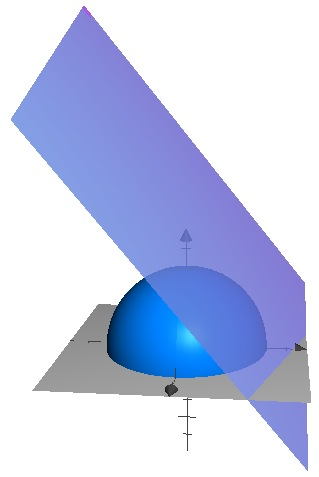
\includegraphics[width=1in]{02sphere-with-tangent.jpg}}

\subsection{Example} \textit{ Find the linear approximation of $F(x, y, z) =
  e^{-y}(x-z)^2$ and tangent plane to its level set at $x=1, y=2, z=5$}
\label{sec:01tangentplane2levelsurface}

\textit{Solution: } At the given values of $x, y, z$ on has $F(1, 2, 5) =
e^{-2}(1-5)^2 = 16/e^2$.  The partial derivatives of $F$ are
\[
F_x = 2(x-z)e^{-y}, \quad F_y = -e^{-y}(x-z)^2, \quad F_z = -2(x-z)e^{-y},
\]
which at $(x, y, z) = (1, 2, 5)$ reduces to $F_x = -8/e^2$, $F_y = -16/e^2$ and
$F_z = +8/e^2$.  If $(x, y, z)$ is close to $(1, 2, 5)$, then the linear
approximation formula tells us that
\[
F(x, y, z) \approx F(1, 2, 5) -\frac8{e^2} (x-1) -\frac{16}{e^2} (y-2) +
\frac8{e^2} (z-5)
\]
or, in ``$\Delta x$'' notation, %
\marginpar{\footnotesize\dfnt%
  By definition:\\
  $\Delta x=x-1$\\
  $\Delta y=y-2$\\
  $\Delta z=z-5$ }
\[
F(1+\Delta x, 2+\Delta y, 5+\Delta z) \approx F(1, 2, 5) -\frac8{e^2} \Delta x
-\frac{16}{e^2} \Delta y + \frac8{e^2} \Delta z.
\]
The equation for the tangent plane to the level set of $F$ at the point
$(1,2,5)$ is therefore
\[
-\frac8{e^2} (x-1) -\frac{16}{e^2} (y-2) + \frac8{e^2} (z-5)=0,
\]
or, after cancelling ${e^2}$'s and $8$'s: $(x-1) + 2(y-2) -(z-5) = 0$.  Further
simplification shows that the equation for the tangent plane is
\[
x+2y-z = 0.
\]

\section{Implicit Functions}
In first semester calculus we learned a procedure for finding derivatives of
implicitly defined functions.  If some function $y=f(x)$ was not given by an
explicit formula, but rather by an implicit equation
\begin{equation}
  F(x, y)=0
  \label{eq:implicit}
\end{equation}
then there was a way to find the derivative of $y=f(x)$ from the above equation
only.  But there was no formula for $f'(x)$.  The reason is that the formula for
the derivative $f'(x)$ involves the partial derivatives of $F$.

In this section we review implicit differentiation again.  The following theorem
is about the zero set of the function $F$.  One usually thinks of the zero set
of a function of two variables as a curve (``an equation defines a curve'') but
this is not always so.  The theorem below gives us a way to find out if the zero
set is really a curve, at least near any given point on the zero set which we
happen to know.

\begin{figure}[ht]
  \centering
  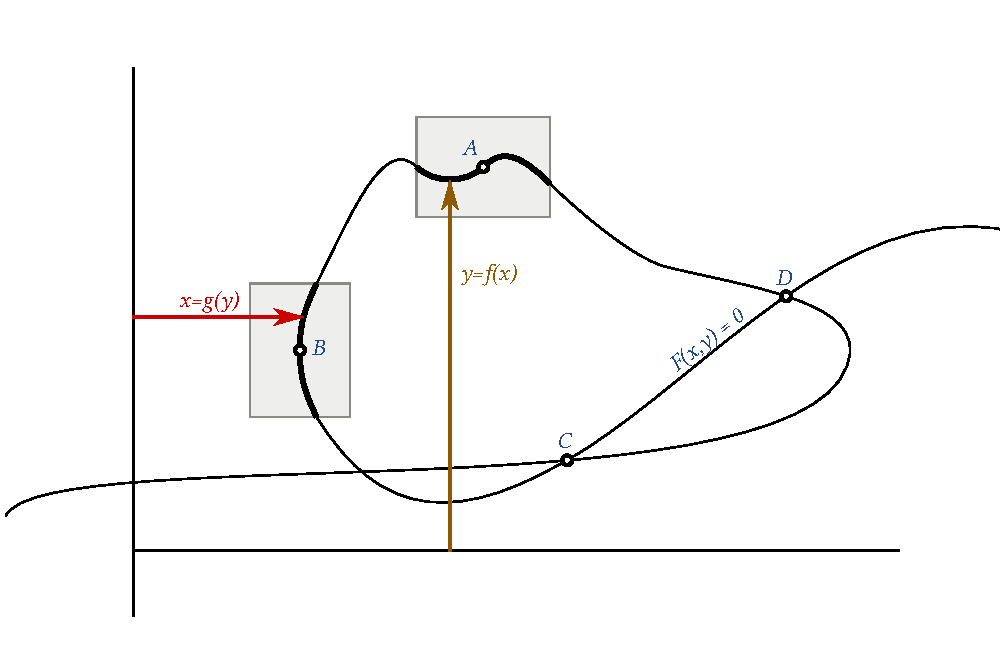
\includegraphics[scale=0.7]{01implicitfunctiontheorem.pdf}
  \caption{ \textbf{The Implicit Function Theorem. } The zero set of a function
    $F(x, y)$ does not have to be the graph of a function, but if at some point
    ($A$) on the zero set we have $F_y\neq0$, then, near that point $A$, the
    zero set is the graph of a function $y=f(x)$.  If $F_x\neq0$ at some point
    ($B$), then near $B$ the zero set is also the graph of a function, provided
    we let $x$ be a function of $y$: $x=g(y)$.\\
    \null\quad\textbf{Exceptional points:} At
    some points, like $C$ and $D$ in this figure, the level set of $F$ cannot be
    represented as the graph of a function $y=f(x)$, nor can it be represented
    as a graph of the type $x=g(y)$.  At such points the Implicit Function
    Theorem implies that both $F_x=0$ and $F_y=0$. }
\end{figure}

\subsection{The Implicit Function Theorem}\itshape
\label{thm:01implicit-function}
Let $F(x, y)$ be a function defined on some plane domain with continuous partial
derivatives in that domain, and suppose that a point $(x_0, y_0)$ in the zero
set of $F$ is given.

If $\pdd Fy (x_0, y_0) \neq 0$ then there is a small rectangle centered at
$(x_0, y_0)$ such that within this rectangle the zero set of $F$ is the graph of
a function $y=f(x)$.  The derivative of this function is
\begin{equation}\label{eq:IFTdydx}
  f'(x) = \frac{dy}{dx} = -\frac{F_x(x, f(x))}{F_y(x,f(x))}.
\end{equation}

If $\pdd Fx (x_0, y_0) \neq 0$ then there is a small rectangle centered at
$(x_0, y_0)$ such that within this rectangle the zero set of $F$ is the graph of
a function $x=g(y)$.  The derivative of this function is
\begin{equation}\label{eq:IFTdxdy}
  g'(y) = \frac{dx}{dy} = -\frac{F_y(g(y), y)}{F_x(g(y),y)}.
\end{equation}


\upshape

A proof may be given in class, time permitting.

There is no need to memorize the formulas \eqref{eq:IFTdydx} and
\eqref{eq:IFTdxdy}.  We can get them by using the method of implicit
differentiation from math 221.  For instance, suppose that the graph of the
function $y=f(x)$ gives you a piece of the zero set of $F$.  This means that
\[
F(x, f(x)) = 0 \text{ for all $x$.}
\]
Differentiating both sides of this equation leads us via the chain rule,
\[
\frac{d F(x, f(x))}{dx} = \pdd Fx (x, f(x)) \cdot \frac{dx}{dx} + \pdd Fy (x,
f(x)) \cdot \frac{df(x)}{dx},
\]
to
\begin{equation}
  0 = \frac{d F(x, f(x))}{dx}
  =F_x(x, f(x)) + F_y(x, f(x)) f'(x).
  \label{eq:IFTdydx-derivation}
\end{equation}
Solve this for $f'(x)$ and we get
\[
f'(x) = \frac{dy}{dx} = -\frac{F_x(x, f(x))}{F_y(x, f(x))},
\]
which is what the theorem claims.

\subsection{The Implicit Function Theorem with more variables}     
There are many variations and extensions of Theorem
\ref{thm:01implicit-function}.  The simplest is to consider the level set of a
function of three rather than two variables.  Suppose $F$ is a function of three
variables, with continuous partial derivatives, and consider the set of points
defined by the equation
\[
F(x, y, z) = C.
\]
This is the level set of $F$ at level $C$.

If
\[
\pdd F y (x_0, y_0, z_0) \neq 0,
\]
then near $(x_0, y_0, z_0)$ the level set of $F$ is the graph of a function
$y=g(x, z)$, meaning that the function $y=g(x, z)$ satisfies
\[
G(x, g(x, z), z) = 0.
\]
Hence we can find the partial derivatives of this function by implicit
differentiation.  The result is
\begin{equation}
  \pdd yx = g_x(x, z) = - \frac{F_x(x, y, z)}{F_y(x, y, z)},\qquad
  \pdd yz = g_z(x, z) = - \frac{F_z(x, y, z)}{F_y(x, y, z)},
  \label{eq:IFTxyz}
\end{equation}
where $y=g(x, z)$.

\subsection{Example -- The saddle surface again}     
The saddle surface is the graph of the function $z=xy$, which we can think of as
the zero set of the function
\[
F(x, y, z) = z- xy.
\]
The point $(2, 3, 6)$ lies on the saddle surface, and at this point the partial
derivatives of $F$ are
\[
F_x =\frac{\pd(z-xy)}{\pd x} = -y = -3, \quad 
F_y =\frac{\pd(z-xy)}{\pd y} = -x = -2, \quad 
F_z =\frac{\pd(z-xy)}{\pd z} = 1.
\]
Since $F_x(2, 3, 6) = -3 $ is non zero, the Implicit Function Theorem tells us
that near this point the zero set of $F$ is the graph of a function $x=g(y, z)$.
Solving $F=0$ for $x$ we see that this function is in fact
\[
x= g(y, z) = \frac{z}{y}.
\]
The partial derivatives of $g$ are easy to compute in this example, but even if
we couldn't find them directly, the Implicit Function Theorem would tell us that
\[
g_y(3, 6) = -\frac{F_y(2, 3, 6)}{F_x(2, 3, 6)} = \frac{2}{3},\qquad 
g_z(3, 6) = -\frac{F_z(2, 3, 6)}{F_x(2, 3, 6)} = \frac{1}{3}.
\]

\section*{Problems}
\begin{multicols}{2}
\problemfont
\problem Compute the gradient of each function in 
Problem~\ref{prb:01compute-these-partials} of
\S~\ref{sec:partial-derivative-problems}.

\problem\label{prb:prodrule-for-grad} 
Show that for any two differentiable functions $f$ and $g$ one has
\begin{align*}
  \nab(f\pm g) &= \nab f \pm \nab g,\\
  \nab (fg) &= f\nab g+ g\nab f,\\
  \nab \bigl(\frac fg\bigr) &= \frac{g\nab f - f\nab g} {g^2}.
\end{align*}
In other words the sum-, product- and quotient rules for differentiation
also apply to the gradient.
\answer
$\pdd{(f+g)}x = f_x + g_x$, and $\pdd{(f+g)}y = f_y + g_y$, so 
\[
\vek\pdd{(f+g)}x \\ \rule{0pt}{18pt}\pdd{(f+g)}y \tor
= \vek f_x + g_x \\ f_y + g_y\tor
= \vek f_x \\ f_y\tor + \vek g_x \\g_y\tor
\]
Hence $\nab(f+g) = \nab f + \nab g$.

The product and quotient rules follow in the same way.
\endanswer

\problem \subprob Draw the level sets of the function 
$f(x,y) = x^2 + 4y^2$ at levels $0$, $4$, $16$.


\subprob Find the points on the level set $f(x,y) = 4$ where the
gradient is parallel to the vector $\tvek 1\\1\ttor$.  What can you
say about the tangent line to the level set at those points?  Draw the
gradient vectors, and the tangent lines at the points you just found.

\textbf{Hint: } two non-zero vectors $\vv$ and $\vw$ are parallel if
there is a number $s$ such that $\vv = s\vw$.
\answer
The gradient is $\nab f = \tvek 2x \\ 8y\ttor$.  This vector is
parallel to $\tvek1\\1\ttor$ if there is a number $s$ such that
$\nab f = s\tvek1\\1\ttor$, i.e.\ $\tvek f_x \\f_y\ttor  = \tvek
s\\s\ttor$.  This happens if $f_x(x, y) = f_y(x, y)$.  From our
computation of the partial derivatives of $f$ we find that $\nab f$ is
parallel to $\tvek1\\1\ttor$ when $2x=8y$.  This happens at every
point on the line $y=\tfrac14x$. 

We are asked which points on the level set $f=4$ satisfy this
condition, so we must find where the line $y=\frac14x$ intersects the
level set $x^2 + 4y^2 = 4$.  Solving the two equations gives two
points $(\frac45\sqrt{5}, \frac15\sqrt{5})$ and $(-\frac45\sqrt{5},
-\frac15\sqrt{5})$.

\endanswer

\subprob Repeat the same two problems for the function $g(x,y) = 4xy^2$.
\answer
$\nab g = \tvek 4y^2 \\ 8xy\ttor$.  This is parallel to
$\tvek1\\1\ttor$ when $y=2x$.  This line intersects the level set
$g=4$ in the point $(\frac12\sqrt[3]{2},\sqrt[3]{2})$.

\textbf{Note: } when you solve the equations $\nab g = \tvek s\\s\ttor$, you
find $y=2x$, but also the line $y=0$ ($x$-axis).   
On this line the gradient actually vanishes, i.e.\ $\nab g = \vvv0$
and has no direction, so you can't really say it is parallel to
$\tvek1\\1\ttor$.
\endanswer


\problem
\subprob Draw the zero set of the function $f(x, y, z) = x^2+y^2-2z$.
\answer
It's a paraboloid of revolution.  
\endanswer

\subprob Find all points on the zero set of the function $f$ where the
gradient is parallel to the vector $\vv = \tvek1\\1\\2\ttor$.
\answer
$\nab f = \tvek2x\\2y\\-2\ttor = s \tvek1\\1\\2\ttor$ if $-2 = 2s$,
i.e.\ $s=-1$.  This then implies $2x= -1$, $2y = -1$, so that
$x=y=-\frac12$.  Since the point has to lie on the zero set of
$f$, we find $z= \frac12(x^2+y^2) = \frac14$.
\endanswer

\problem A bug is crawling on the surface of a hot plate, the temperature 
of which at the point $x$ units to the right of the lower left corner and
$y$ units up from the lower left corner is given by $T(x,y)=100-x^2-3y^3$.

\subprob If the bug is at the point $(2,1)$, in what direction should it
move to cool off the fastest?  
\answer
At $(2,1)$ the gradient is $\nab T = \tvek -2x \\\ -9y^2\ttor =
\tvek-4 \\ -9\ttor$.  To cool off as fast as possible the bug should
go in the opposite direction, i.e.\ in the direction of $\tvek 4 \\
9\ttor$, or any positive multiple of this vector.

\endanswer

\subprob If the bug is at the point $(1,3)$, in what direction should it
move in order to maintain its temperature?
\answer 
At $(1,3)$ the gradient is $\nab T = \tvek -2 \\ -81\ttor$.
To keep its temperature constant the bug should walk in any direction
perpendicular to the gradient.  The vector $\tvek 81 \\ -2\ttor$ is
perpendicular to the gradient, so the bug should go in the direction
of $\tvek 81 \\ -2\ttor$ or the opposite direction, $\tvek -81 \\ 2\ttor$.

Any non-zero multiple of $\tvek -81 \\ 2\ttor$ is also a valid answer,
since we can only give the \textit{direction} and not the speed.

Remember: the vector $\tvek -b\\a\ttor$ is perpendicular to
$\tvek a\\b\ttor$.

\endanswer



\problem The level sets of a function $z=f(x, y)$ are often curves. 
Must they always be curves? Could the zero set of a function be a
solid square (e.g.\ all points $(x,y)$ with $0\le x\le1$ and
$0\le y\le1$)?
\answer
The zero set doesn't have to be a curve.  For example the zero set of
the function $f(x, y) = $distance from $(x,y)$ to the square
$Q$ (Problems \ref{prb:distance-to-square-level-sets} and
\ref{prb:distance-to-square-partialderivs}) is the whole square $Q$.
\endanswer


\problem The caption of Figure~\ref{fig:gradientANDlevels} says that one can only see the direction, but not the length of the gradient $\nab f$ of a function, from just one of its level sets.  It is however possible to see where the gradient is larger from a drawing of several level sets.  We can read this information from the way in which level sets are more bunched together in some regions than in others.

\begin{center}
  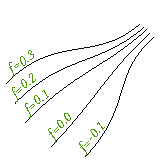
\includegraphics[scale=1.5]{01howBigIsTheGradient.pdf}
\end{center}

The picture above shows some level sets of a function.  On the
bottom left the level sets are further apart, on the top right they
are more bunched together.  Where is the gradient the larger, i.e.~where 
is $\|\nab f\|$ larger: bottom-left, or top-right? 
\answer
$\|\nab f\|$ is larger at the top right, because there the
function $f$ changes faster.
\endanswer

\problem Have a look at Figure~\ref{fig:gradientANDlevels}.  Assume the 
function differentiable at the origin.

\subprob What can you say about the gradient $\nab f$ at the origin?
\answer
The gradient at the origin is the zero vector.  This was explained in the text.
\endanswer

\subprob Where is the function positive and where is it negative
(assume that the whole zero set is drawn).
\answer
The function increases in the direction of the gradient.  Since it vanishes on the curve in Figure~\ref{fig:gradientANDlevels}, the function will be positive in the region above the curve, and it will be negative both below the curve and inside the little loop.
\endanswer

\problem  This problem asks you to think about the Implicit Function Theorem~\ref{thm:01implicit-function}

Consider the unit circle $\setC$ with equation
\[
x^2+y^2=1.
\] 
The unit circle $\setC$ is a level set of the function $F(x,y) = x^2+y^2$.

\subprob Where on $\setC$ is $F_y \neq0$?  Near which points $P$ on $\setC$ can one
represent $\setC$ as a graph of the form $y=f(x)$?

\subprob Near which points $P$ on $\setC$ can one represent $\setC$ as a graph of
the form $x=g(y)$?


\problem  Here is the zero set of a function $z=f(x, y)$ (in bold). 
The function is only zero on the bold curve, it is nonzero everywhere
else.
\begin{center}
  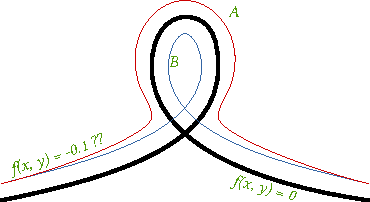
\includegraphics[width=0.4\textwidth]{01LevelSetProblem1.pdf}
\end{center}

\subprob One of the two other curves above is the level set $f(x, y) =
-0.1$.  Which one is it, $A$ or $B$?  As always, explain your answer.

\subprob Draw a possible level set $f(x, y) = +0.1$.

\subprob Draw possible gradients on the zero set (similar to
Figure~\ref{fig:gradientANDlevels}).

\problem Here is the zero set of a differentiable function $z=f(x, y)$. 
\begin{center}
  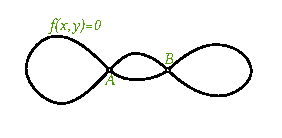
\includegraphics[width=0.4\textwidth]{01findthecriticalpoints.pdf}
\end{center}
Explain why the Implicit Function Theorem (\S
\ref{thm:01implicit-function}) implies that $\nab f=\vvv0$ at the two points
$A$ and $B$.
%
% \subprob Consider the function $g(x, y) = f(x,y)^2$.  Show that $f$ and $g$
% have the same zero set.
%
% \subprob Show that $\nab g = 2f\nab f$.  (Hint: look at problem
% \ref{prb:prodrule-for-grad}).
%
% \subprob Show that $\nab g=\vvv0$ at \emph{all} points on the zero set of $g$.
%
\problem \subprob Compute the gradient of the ``distance to the square 
function'' $f$ from problems \ref{prb:distance-to-square-level-sets}
and \ref{prb:distance-to-square-partialderivs}.

\subprob How much is $|\nab f|$?
\answer
The result of a rather long calculation is that $\|\nab f\| =1$ everywhere outside the 
square, and $\|\nab f\| = 0$ inside the square
(because $f$ is constant in the square.)
\endanswer

\subprob  Make a drawing of the level sets of $f$, and the gradient
$\nab f$.



\problem Let $f(x, y) = \ln(2+2x+e^y)$. 

\subprob Compute the gradient of $f$ at the point $(x_0, y_0)$ with
position vector $\vx_0 = \tvek 1 \\ 0\ttor$.  

\subprob You are allowed to choose a point at a distance $0.01$ from
the point $(1,0)$.  Where would you choose the new point if you want
$f$ to be as large as possible?  (Hint:  review the linear
approximation formula and subsequent discussion about the gradient as
direction of greatest increase in
\S\ref{sec:01grad-is-direction-of-greatest-increase})

\subprob Is your answer to the previous the \textit{exact} answer, or only an
\textit{approximation}?  I.e.,\ could someone else find a point at distance
$0.01$ from $(1,0)$ at which $f$ has a (slightly) higher value than at
the point you found?

\subprob The level set $C$ of $f$ through the point $(1,0)$ happens to be the
graph of a function $y=g(x)$.  Find that function.

\subprob Find a normal vector to the tangent line to $C$ at the point
$(1,0)$.  Find an equation for the tangent line to $C$ at $(1,0)$.  

\subprob How much is $g(1)$?  Find two different ways to compute
$g'(1)$ based on the work you have done so far.


\problem Let $(a,b,c)$ be a point on the sphere with radius $R$ 
centered at the origin.  Find an equation for the tangent plane to the
sphere at $(a,b,c)$.
Simplify your answer as much as possible ($a, b, c$, and $R$ will show
up in your answer of course.)
\answer
$ax+by+cz = R^2$.
\endanswer
% \immediate\write\ans{\string\newpage}
\noproblemfont
\end{multicols}

\section{The Chain Rule with more Independent Variables;\\ Coordinate Transformations}
The chain rule we have seen so far tells us how to differentiate expressions of
the form $f(x(t), y(t))$.  Such expressions are the result of substituting two
functions $x(t), y(t)$ of one variable $t$ in one function of two variables
$z=f(x, y)$.  What do we do if the functions $x, y$ that get substituted in
$f(x, y)$ depend on not one, but two (or more) variables?  The answer is easy:
\emph{we do exactly the same.  }

For instance, suppose we want to substitute $x=x(u,v)$ and $y=y(u,v)$ in a
function $z=f(x, y)$, resulting in a function $F(u,v) = f(x(u,v), y(u,v))$, and
suppose we want find the partial derivatives of $F$ with respect to $u$.  To
compute this we \textit{keep $v$ fixed} and regard $u$ as the variable -- then
$x(u, v)$ and $y(u, v)$ are functions of one variable $u$ and we apply the chain
rule we already know.  This leads to
\[
\pdd Fu = \pdd fx \pdd xu + \pdd fy \pdd yu
\]
The only difference with \eqref{eq:chain-rule} is that we have written the
derivatives of $x$ and $y$ as partial derivatives.  We do this to indicate that
in computing this derivative we momentarily consider $x$ as a function of $u$,
but later we may want to vary $v$ again.

The same considerations lead to the partial derivative of $F$ with respect to
$v$:
\[
\pdd Fv = \pdd fx \pdd xv + \pdd fy \pdd yv.
\]
\subsection{An example without context}
Suppose $f$ is some function of two variables and we want to find the partial
derivatives of
\[
g(u, v, w) = f(2uv, u^2+w^2).
\]
By this we mean that $g$ is the result of substituting $x= 2uv$ and $y=u^2+w^2$
in $f$.  Note that $g$ is a function of three vairables, and $f$ is a function
of two variables.

The chain rule tells us that the derivatives of $g$ are
\begin{align*}
  \pdd gu &= \pdd fx\pdd xu +\pdd fy \pdd yu = 2v\pdd fx + 2u\pdd fy\\
  \pdd gv &= \pdd fx\pdd xv +\pdd fy \pdd yv = 2u\pdd fx \\
  \pdd gw &= \pdd fx\pdd xw +\pdd fy \pdd yw = 2w\pdd fy
\end{align*}


\subsection{Example: a rotated coordinate system}
\label{sec:01rotated-coordinates}

\begin{figure}[b]
  \centering
  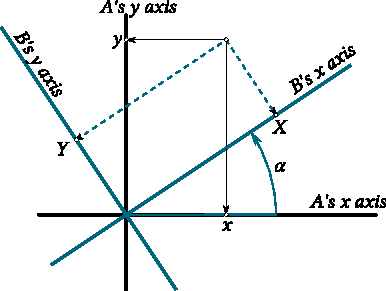
\includegraphics{01coordinatesRotated.pdf}
  \caption{After choosing different $x$ and $y$ axes, A and B will assign
    different $x, y$ coordinates to the same point in the plane.  Equations
    \eqref{eq:coordinateRotation} give the relation between these two sets of
    coordinates. }
  \label{fig:coordinateRotation}
\end{figure}

We are used to specifying the location of points in the plane by giving their
$x$ and $y$ coordinates, but sometimes it is better to use different
coordinates.  For instance, two people A and B could have chosen the same
origin, but their axes could be rotated with respect to each other. See
Figure~\ref{fig:coordinateRotation}.  If A's coordinates are called $x,y$ and
B's coordinates are $X,Y$ then it should be possible to find A's coordinates of
a point if we know what coordinates B assigns to this point -- given $X,Y$ what
are $x,y$?  The answer to this question is\footnote{One way of arriving at these
  relations is to use vectors as in the first vector work sheet of this
  semester.}
\begin{equation}\label{eq:coordinateRotation}
  \left\{
    \begin{aligned}
      x = X\cos\alpha - Y\sin\alpha,\\
      y = X\sin\alpha + Y\cos\alpha.
    \end{aligned}
  \right.
\end{equation}
Suppose both A and B are measuring the temperature $T$ at various points in the
plane.  A predicts the temperature at various points in the plane: he says that
at the point with coordinates $(x,y)$ the temperature will be $T(x, y)$.  In
fact he has also found the partial derivatives $\pdd {T}x $ and $\pdd {T}y $.

Equipped with the $X,Y \to x,y$ conversion \eqref{eq:coordinateRotation} B can
now take A's formula for the temperature and express it in terms of her own
$X,Y$ coordinates.  If we write $T_A(x, y)$ for the temperature at the point
whose A-coordinates are $(x,y)$ and $T_B(X,Y)$ for the temperature at the point
whose B-coordinates are $(X,Y)$, then we have
\begin{align*}
  T_B(X,&Y) = T_A(x,y)\\
  &= T_A(X\cos\alpha - Y\sin\alpha, X\sin\alpha + Y\cos\alpha).
\end{align*}
What is the relation between the partial derivatives of the temperatures as
computed by A and by B?  The chain rule gives the answer:
\begin{align*}
  \frac{\pd T_B}{\pd X} &= \pdd{}X\Bigl\{ T_A\bigl(\underbrace{X\cos\alpha -
    Y\sin\alpha}_{=x},
  \underbrace{X\sin\alpha + Y\cos\alpha}_{=y} \bigr)\Bigr\}\\
  &= \frac{\pd T_A}{\pd x} \cos\alpha + \frac{\pd T_A}{\pd y}\sin\alpha.
\end{align*}
\subsection{Another example -- Polar coordinates}
\label{sec:Chain-rule-polar-coordinates}
Suppose a quantity $P$ is given in terms of Cartesian coordinates $x$ and $y$:
$P=f(x, y)$.  How does $P$ change if we vary the polar coordinates $r$ and
$\theta$, i.e.\ what are the partial derivatives of $P$ with respect to $r$ and
$\theta$?

To answer this question we must write $P$ as a function of $r$ and $\theta$.
Recall that the relation between Cartesian coordinates and polar coordinates is
\begin{equation}\label{eq:polar-to-cartesian}
  x = r\cos \theta, \qquad y= r\sin \theta.
\end{equation}
Therefore $P=f(x, y) = f(r\cos \theta, r\sin \theta)$ and we get
\begin{equation}
  \pdd Pr = \cos \theta \pdd fx + \sin \theta \pdd fy,
  \qquad
  \pdd P \theta = 
  -r\sin \theta\pdd fx + r\cos \theta \pdd fy
\end{equation}
Since the function $f$ always gives us the value of the quantity $P$, these
relations are usually written in this way:
\begin{equation}
  \pdd Pr = \cos \theta \pdd Px + \sin \theta \pdd Py,
  \qquad
  \pdd P \theta = 
  -r\sin \theta\pdd Px + r\cos \theta \pdd Py
\end{equation}
Using the relation \eqref{eq:polar-to-cartesian} between polar and Cartesian
coordinates we can write these equations in yet another way:
\begin{equation}
  \pdd Pr = \frac xr \pdd Px + \frac yr \pdd Py,
  \qquad
  \pdd P \theta = -y \pdd Px + x \pdd Py
\end{equation}

 

\section{Problems}
\begin{multicols}{2}
\problemfont


\problem Use the chain rule to compute $dz/dt$ for 
$z=\sin(x^2+y^2)$, $x=t^2+3$, $y=t^3$.
\answer
$4xt\cos(x^2+y^2)+6yt^2\cos(x^2+y^2)$
\endanswer

\problem Use the chain rule to compute $dz/dt$ for 
$z=x^2y$, $x=\sin(t)$, $y=t^2+1$.
\answer
$2xy\cos t+2x^2t$
\endanswer

\problem Use the chain rule to compute $\partial z/\partial s$ and  
$\partial z/\partial t$ for
$z=x^2y$, $x=\sin(st)$, $y=t^2+s^2$.
\answer
$2xyt\cos(st)+2x^2s$, $2xys\cos(st)+2x^2t$
\endanswer

\problem Use the chain rule to compute $\partial z/\partial s$ and  
$\partial z/\partial t$ for
$z=x^2y^2$, $x=st$, $y=t^2-s^2$.
\answer
$2xy^2t-4yx^2s$, $2xy^2s+4yx^2t$
\endanswer


\problem\subprob Let $x=x(u,v), y=y(u,v)$ be  the following set of
functions of $u, v$:
\[
x=u^2-v^2,\quad y=2uv.
\]
If $g(u,v) = f(x(u,v), y(u,v))$ then compute $g_u(1,0)$,
$g_u(1,1)$, $g_v(1,0)$, and $g_v(1,1)$, if you are given these values
of the partial derivatives of $f$:

\begin{center}
  \begin{tabular}{cc|cc}
    $x$  & $y$  & $f_x(x, y)$ & $f_y(x, y)$ \\  \hline
    0 & 0 & $A$ & $B$\\
    1 & 0 & $C$ & $D$\\
    0 & 1 & $E$ & $F$\\
    1 & 1 & $G$ & $H$\\
    2 & 0 & $I$ & $J$\\
    0 & 2 & $K$ & $L$
  \end{tabular}
\end{center}

\subprob Repeat the above problem if $x$ and $y$ are given by $x=u$, $y=v/u$.

\subprob Repeat part \textbf{(a)} of this problem if $x$ and $y$ are given by $x=u+v$, $y=u-v$.

\problem Let $x, y, X, Y, T_A$, and $T_B$ be as in the example in 
\S\ref{sec:01rotated-coordinates}.  In that section we computed
$\pdd{T_B}X$.  

\subprob Compute $\DS\pdd{T_B}{Y}$.
\answer
$\pdd{T_B}{Y} = -\sin\alpha \pdd{T_A}{x} + \cos\alpha \pdd {T_A}{y}$.
\endanswer

\subprob Show that 
\[
\bigl(\pdd{T_A}x\bigr)^2+
\bigl(\pdd{T_A}y\bigr)^2=
\bigl(\pdd{T_B}X\bigr)^2+
\bigl(\pdd{T_B}Y\bigr)^2.
\]
In other words, A and B may measure different partial derivatives, but
the temperature gradients they find have the same length.
$\|\nab T_A\| = \|\nab T_B\|$.
\answer
Take the formulas for $\pdd{T_B}X$ and $\pdd{T_B}Y$ and work out the
right hand side in this problem.
\endanswer

\problem (About polar coordinates). In \S\ref{sec:Chain-rule-polar-coordinates} we saw how we can use the chain rule to find $\pdd fr$ and $\pdd f\theta$ if we know the function $f$ in terms of Cartesian coordinates $(x,y)$.  In this problem we turn the question around: suppose we are given a function in polar
coordinates, how do we compute its gradient.

Recall that polar and Cartesian coordinates are related by
\[
r=\sqrt{x^2+y^2}
\text{ and }
\theta = \arctan \frac yx,
\]
at least in the region where $x>0$. (See Chapter III, \S~\ref{sec:functions-in-PC}.)

\subprob Compute $\pdd rx$, $\pdd ry$, $\pdd\theta x$, $\pdd\theta y$.
Try to simplify your answer as much as possible, by reusing the
variables $r$ and $\theta$.  For instance, the simplest way to write
$\pdd rx$ is as $\pdd rx= \frac{x} {r}$.


\subprob Suppose a quantity $P$ is given in terms of Polar coordinates
by $P= f(r, \theta)$.  Express $\pdd Px$ and $\pdd Py$ in terms of
$\pdd fr$ and $\pdd f\theta$.  

More precisely, compute
\[
 \pdd Px \stackrel{\sf def}= \pdd {\bigl\{f(r(x,y), \theta(x,y)\bigr\}} {x}
\]
and
\[
 \pdd Py \stackrel{\sf def}= \pdd {\bigl\{f(r(x,y), \theta(x,y)\bigr\}} {y}
\]

\subprob Show that
\[
\|\nab P\|^2 = \bigl(\pdd fr\bigr)^2 + \frac{1} {r^2}\bigl(\pdd f\theta\bigr)^2.
\]

\problem For some function $f$ we are told that at the point 
with Cartesian coordinates $(4,3)$ one has 
\[
\pdd fr = 3, \quad \pdd f\theta = 6.
\]
Compute the gradient $\nab f$ at $(2,1)$.

\problem In physics an electric field is described by its \emph{potential 
  function}, $\phi=\phi(x,y)$ (in this problem we assume the world is
two-dimensional; the potential $\phi$ is measured in Volts).  Minus the
gradient of the potential function is called the \emph{electric field:}
\[
\vE = - \nab \phi.
\]
The electric potential of a point charge in the plane is given in Polar
coordinates by $\phi = -C\ln r$, for some constant $C$ (the physicists will
tell you that $C$ depends on the charge that was placed at the origin; for
us it is just some number, and we will in fact assume that $C=1$.)

\subprob Compute the electric field $\vE$ corresponding to the potential $\phi
= -\ln r$.
\answer $\vE = -\nab \ln r = \frac{1} {r^2}\tvek x\\ y\ttor$.
\endanswer

\subprob Compute $\| \vE\|$ (this quantity measures the strength of the
electric field, but not its direction.)  Where is the electric field
stronger?
\answer $\|\vE\| = 1/r = \frac{1} {\sqrt{x^2+y^2}}$.
\endanswer

\subprob Make a drawing of the level curves of the potential $\phi$, and the
electric field $\vE$.  

\subprob In the three dimensional world the electric potential generated by
a charged particle at the origin is not given by $-C\ln r$, but instead by
the so-called \textit{Coulomb potential}
\[
\phi = \frac{C} {r}, \text{ where } r= \sqrt{x^2+y^2+z^2}.
\]
Compute the corresponding electric field $\vE = -\nab \phi$.

\problem The {\em ideal gas law\/}, given by $PV=nRT$, relates the 
Pressure, Volume, and Temperature of $n$ moles of gas.  ($R$ is the
ideal gas constant).  Thus, we can view pressure, volume, and
temperature as variables, each one dependent on the other two.

(In this problem pressure is measured in Pascals, temperature in degrees
Kelvin, and volume in Liters.)

Each of the following three questions can be answered by applying the
chain rule to differentiate $z(t) = f(x(t), y(t))$ for suitable
quantities  $x$, $y$, and $z$.  In each case state which variables
play the role of $x, y, z$, and what the function $f$ is.

\subprob If pressure of a gas is increasing at a rate of $0.2
\text{Pa}/\text{min}$ and temperature is increasing at a rate of $1
^\circ\text{K}/\text{min}$, how fast is the volume changing?

\subprob If the volume of a gas is decreasing at a rate of $0.3
\text{L}/\text{min}$ and temperatuere is increasing at a rate of $0.5^\circ
\text{K}/\text{min}$, how fast is the pressure changing?

\subprob If the pressure of a gas is decreasing at a rate of $0.4
\text{Pa}/\text{min}$ and the volume is increasing at a rate of $3
\text{L}/\text{min}$, how fast is the temperature changing?

\problem The ideal gas law says $PV=nRT$, where $P,V,T$ are variables, 
and $n$, $R$ are constants.  Verify the following identity: 
\[
  {\partial P\over \partial V} {\partial V\over \partial T}
{\partial T\over \partial P}=-1
\]

\problem The previous exercise was a special case of the following 
fact, which you are asked to verify here:

Assume that $F(x,y,z)$ is a function of 3 variables, and suppose that
the relation $F(x,y,z)=0$ defines each of the variables in terms of
the other two, namely $x=f(y,z)$, $y=g(x,z)$ and $z=h(x,y)$, then
\[
\pdd xy \pdd yz \pdd zx =-1.
\]
Hint: this is a problem about implicit differentiation.


\problem
Four cartographers are using different coordinates to describe the
same landscape.  Each of them describes the landscape by specifying a
the height of a point in the landscape as a function of its position
above a horizontal plane.

Cartographer A uses Cartesian coordinates $(x, y)$ in the plane, B
uses Cartesian coordinates $(X,Y)$ in the plane.
The coordinates $(X,Y)$ are rotated by $45^\circ$ with respect to 
$(x, y)$ (see \S\ref{sec:01rotated-coordinates}).  

Cartographer C works with A but uses polar coordinates $(r, \theta)$
($r$ is the distance to the origin, $\theta$ is the angle with A's
$x$-axis).  

Cartographer D works with B and uses polar coordinates $(r, \varphi)$ 
($r$ is the distance to the origin, $\varphi$ is the angle with B's
$X$-axis).  

Here is a picture of the landscape that A, B, C, and D are
looking at:

\begin{center}
  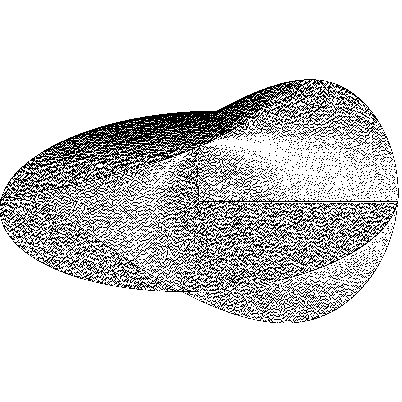
\includegraphics[width=0.3\textwidth]{01disco.pdf}
\end{center}

\subprob If B has found that the height is given by the function 
$f(X, Y) = 2XY/(X^2+Y^2)$, then what function does A find for the
height?
\answer
Height $ = - (x^2-y^2)/(x^2+y^2)$
\endanswer

\subprob What height function does C find?
\answer
Height $ = \sin 2\theta$.
\endanswer

\subprob What height function does D find?
\answer
Height $ = \cos 2\varphi$.
\endanswer

\problem Brian and Ally are using different Cartesian coordinate 
systems in the plane: $(x, y)$ for Ally, $(X,Y)$ for Brian.  They have
the same origin, but Brian's coordinates are rotated by an angle of
$\theta = \arctan \frac43$ ($\approx 53^\circ$, although that is only an
approximation.  You can give exact answers in this problem, and you
don't need a calculator.)

\subprob What is the relation between $(x,y)$ and $(X, Y)$?

\subprob If Ally has found that $T_A(x,y) = 32+0.1y$, then what
formula $T_B(X,Y)$ will Brian use to describe the temperature?

\subprob On a different occasion Ally found that the temperature had
changed.  Now Ally measures the temperature and finds that at the
point with $x=1, y=1$ one has $T_A(1,1) = 35$, and also $\pdd {T_A}x =
0.05$ and $\pdd{T_A}y = 0.8$.  Which coordinates does Brian assign to
this point, which temperature $T_B$, and which derivatives $\pdd
{T_B}X$ and $\pdd{T_B}Y$ does Brian compute at this point?

[Hint: before you compute anything, find $\sin \theta$ and
$\cos\theta$;  also draw a right triangle one of whose acute angles is
$\theta$.]
\noproblemfont

\end{multicols}

\section{Higher Partials and Clairaut's Theorem}

\subsection{Higher partial derivatives}     
By definition
\begin{equation}
  \begin{aligned}
    \frac{\pd ^2 f}{\pd x^2} &= \frac{\DS\pd \bigl(\pdd fx \bigr)}{\pd x}&
    \frac{\pd ^2 f}{\pd x \pd y} &=
    \frac{\DS\pd \bigl(\pdd fy \bigr)}{\pd x}\\
    \frac{\pd ^2 f}{\pd y \pd x} &= \frac{\DS\pd \bigl(\pdd fx \bigr)}{\pd y}&
    \frac{\pd ^2 f}{\pd y^2} &= \frac{\DS\pd \bigl(\pdd fy \bigr)}{\pd y}
  \end{aligned}
  \label{eq:second-partials-defined}
\end{equation}
In subscript notation one writes these higher partial derivatives as follows:
\[
\begin{aligned}
  f_{xx}(x, y) &= \frac{\pd ^2 f}{\pd x^2}&
  f_{xy}(x, y) &= \frac{\pd^2 f}{\pd y \pd x}\\
  f_{yx}(x, y) &= \frac{\pd^2 f}{\pd x \pd y}& f_{yy}(x, y) &= \frac{\pd^2
    f}{\pd y^2}\;.
\end{aligned}
\]
\emph{Note the reversal in $xy$ order in the mixed partial derivatives!}

\subsection{Example} If $f(x, y) = x^2y+\cos xy$ then $ f_x = 2xy - y\sin xy, $
and hence
\begin{eqnarray*}
  f_{xx} & = &
  \frac{\pd (2xy-y\sin xy)}{\pd x}=
  2y - y^2\cos xy,
  \\
  f_{xy} & = &
  \frac{\pd (2xy-y\sin xy)}{\pd y}=
  2x - \sin xy -xy \cos xy.
\end{eqnarray*}
The other partial derivatives follow from $f_y = x^2 - x\sin xy$, and they are
\[
f_{yx} = 2x - \sin xy - xy\cos xy, \quad f_{yy} = -x^2 \cos xy.
\]
Every time we take a derivative, we can choose whether we differentiate with
respect to $x$ or $y$.  Differentiating once we have two possibilities,
differentiating twice we have $2\times2 = 4$ possibilities, etc.  That is why we
found four partial derivatives of second order in the above example.  But if we
look carefully, we also see that $f_{xy}$ and $f_{yx} $ are the same.  This is
no coincidence.

\subsection{Clairaut's Theorem -- mixed partials are equal}     
\label{thm:Clairaut}
\textit{If for a given function $f$ of two variables the mixed partial
  derivative $f_{xy}(x, y)$ exists for all $(x, y)$ in a neighborhood of a point
  $(a,b)$, and if this derivative is continuous at $(a, b)$, then the other
  mixed partial derivative $f_{yx}(a,b)$ also exists, and $f_{xy}(a, b) =
  f_{yx}(a,b)$.  }

So we normally don't have to worry about the order in which we take partial
derivatives.

\subsection{Proof of Clairaut's theorem} With some algebra we can show that the
definition of partial derivatives implies
\begin{multline}
  \label{eq:Clairaut1}
  \frac{\pd^2 f}{\pd x \pd y} = \\
  \lim_{\Delta x\to 0}\lim_{\Delta y\to 0}
  \frac{f(x+\Delta x, y+\Delta y) - f(x, y+\Delta y) - f(x+\Delta x, y) +
    f(x, y)} {\Delta x \Delta y}
\end{multline}
while
\begin{multline}
  \label{eq:Clairaut2}
  \frac{\pd^2 f}{\pd y \pd x} = \\
  \lim_{\Delta y\to 0}\lim_{\Delta x\to 0}
  \frac{f(x+\Delta x, y+\Delta y) - f(x, y+\Delta y) - f(x+\Delta x, y) +
    f(x, y)} {\Delta x \Delta y}
\end{multline}
So it's a matter of showing that one can switch the two limits.  We won't go
into the details here, but the hypothesis that $f_{xy}$ is continuous implies
that we are indeed allowed to switch the limits.

\section{Finding a function from its derivatives} 
\label{sec:finding-f-from-its-derivs}
We now look at integrating
the partial derivatives of a function, which looks out of place here (this being
a chapter on derivatives and not on integrals), but Clairaut's Theorem actually
turns out to play a role.

If we have the derivative $f'(x)$ of some function of one variable then we know
how to recover the function $f(x)$: we integrate, i.e.
\[
f(x) = \int f'(x) dx + C.
\]
Furthermore, any (continuous) function can be the derivative of a function,
because, if someone gives us a continuous function $f(x)$, then
\[
F(x) \stackrel{\rm def}{=} \int_a^x f(t) dt
\]
is a differentiable function whose derivative is $F'(x) = f(x)$.

What about functions of more than one variable?  Suppose we know the partial
derivatives
\begin{equation}\label{eq:potential}
  \pdd fx  = P(x, y) \text{ and }
  \pdd fy  = Q(x, y)
\end{equation}
of a function of two variables, can you then find the function $f(x,y)$?

The answer is ``yes, you can find $f$ by integrating, \emph{if it exists,} but not
every pair of functions $P$ and $Q$ are the partial derivatives of some function.''

The following two examples are typical of what can happen.


\subsection{Example}     
Does there exist a function $f(x, y)$ of two variables such that
\[
\pdd fx = x^3 - 2xy,\text{ and } \pdd fy = 3y^2
\]
both hold?  The answer is no, such a function cannot exist, and here is the
reason: if there were such a function, then we could compute
\[
\frac{\pd^2 f}{\pd y \pd x} = \frac{\pd( x^3 - 2xy)}{\pd y} = -2x, \text { and }
\frac{\pd^2 f}{\pd x \pd y} = \frac{\pd (3y^2)}{\pd x} = 0.
\]
By Clairaut's Theorem both computations should give us the same answer, but they
don't.  Therefore the function $f$ whose partials are as above cannot exist.

\subsection{Example}     
Does there exist a function $f(x, y)$ of two variables whose derivatives are
\[
\pdd fx = x^3 - 2xy,\text{ and } \pdd fy = \sin \pi y - x^2 ?
\]
Let's check Clairaut's condition:
\[
\frac{\pd^2 f}{\pd y \pd x} = \frac{\pd( x^3 - 2xy)}{\pd y} = -2x, \text { and }
\frac{\pd^2 f}{\pd x \pd y} = \frac{\pd (\sin \pi y - x^2)}{\pd x} = -2x.
\]
This time both computations gave us the same answer, so Clairaut's theorem does
not rule out the existence of the function $f$ that we are looking for.  We can
try to compute it by integrating both partial derivatives.  There is a
systematic way of doing this that usually leads to the answer.

We first integrate $f_x$ while treating $y$ as a constant:
\[
f(x, y ) = \int \{x^3-2xy\} \; dx = \tfrac14 x^4 - x^2y + C(y).
\]
The ``constant'' is only a constant in the sense that it does not depend on $x$.
It may depend on $y$, and that is why we wrote it as $C(y)$.  To find $C(y)$ we
differentiate this result with respect to $y$:
\[
\sin\pi y - x^2 = f_y = \frac{\pd \bigl\{ \tfrac14 x^4 - x^2y + C(y)\bigr\}
}{\pd y} = -x^2 + C'(y).
\]
So we see that $C'(y) = \sin\pi y$, and hence $C(y) = -\frac1\pi \cos\pi y + K$,
where $K$ is a real constant ($K$ depends neither on $x$ nor on $y$).

We find that the following function has the prescribed partial derivatives
\[
f(x, y) = \tfrac14 x^4 - x^2y -\tfrac1\pi \cos \pi y + K
\]
where $K$ is constant, i.e.~where $K$ depends on neither $x$ nor $y$.

The method used in this example always works, and we summarize this fact in the
following theorem.
\begin{theorem} Suppose $P(x, y)$ and $Q(x,y)$ are two functions that are
  defined on a rectangular domain $\cR = \{(x, y) : a<x<b, c<y<d\}$, and suppose
  that they have continuous partial derivatives on this domain.

  If a function $f(x, y)$ exists such that \eqref{eq:potential} holds on $\cR$,
  then
  \begin{equation}\label{eq:exact}
    \pdd Py = \pdd Qx
  \end{equation}
  must hold on $\cR$.

  Conversely, if $P$ and $Q$ satisfy \eqref{eq:exact} then there is a function
  $f$ defined on $\cR$ that satisfies \eqref {eq:potential}.
\end{theorem}

\bigskip

To prove this theorem we need to understand integrals of functions of several
variables, and Green's theorem in particular, so this will have to wait until
the end of the semester.  See \S~VII.\ref{sec:clairaut-is-conservative}.

It should be noted that the assumption above that the functions $P$ and $Q$ be
defined on a rectangle is important: the theorem is no longer true if the domain
of $P$ and $Q$ ``has holes.''  See problem \ref{prb:grad-of-theta}.

\newpage
\section{Problems}
\label{sec:partial-deriv-problems}
\begin{multicols}{2}
\problemfont 
\problem Find all first and second partial derivatives of $x^3y^2+y^5$.  
\answer $f_x=3x^2y^2$, $f_y=2x^3y+5y^4$, $f_{xx}=6xy^2$,
$f_{yy}=2x^3+20y^3$, $f_{xy}=6x^2y$
\endanswer

\problem Find all first and second partial derivatives of $4x^3+xy^2+10$.  
\answer
$f_x=12x^2+y^2$, $f_y=2xy$, $f_{xx}=24x$, $f_{yy}=2x$, $f_{xy}=2y$
\endanswer

\problem Find all first and second partial derivatives of $x\sin y$.  
\answer $f_x=\sin y$, $f_y=x\cos y$, $f_{xx}=0$, $f_{yy}=-x\sin y$,
$f_{xy}=\cos y$
\endanswer

\problem Find all first and second partial derivatives of  
$\sin(3x)\cos(2y)$.

\problem Find all first and second partial derivatives of $e^{x+y^2}$.  

\problem Find all first and second partial derivatives of  
$\ln\sqrt{x^3+y^4}$.

\problem Find all first and second partial derivatives of $z$ with respect  
to $x$ and $y$ if $x^2+4y^2+16z^2-64=0$.  (Hint: solve for $z$ or use implicit
differentiation\ldots)

\problem Find all first and second partial derivatives of $z$ with respect  
to $x$ and $y$ if $xy+yz+xz=1$. (Hint: solve for $z$ or use implicit
differentiation\ldots)

\problem How many different second partial derivatives does a function of  
two variables have?  What about a function of three variables?  How many
derivatives of third degree does a function of two variables have?
\answer
A function of two variables has
\[
  f_{xx},\qquad f_{xy}=f_{yx},\qquad f_{yy},
\]
so it has \emph{three} different partial derivatives of second order.

A function of three variables has these partial derivatives:
\[
  \begin{matrix}
    f_{xx} & f_{xy} & f_{xz} \\
    f_{yx} & f_{yy} & f_{yz} \\
    f_{zx} & f_{zy} & f_{zz}
  \end{matrix}
\]
The ones ``below the diagonal'' are the same as corresponding derivatives
above the diagonal, so there are only six different partial derivatives
of second order, namely these:
\[
  \begin{matrix}
    f_{xx} & f_{xy} & f_{xz} \\
    & f_{yy} & f_{yz} \\
    & & f_{zz}
  \end{matrix}
\]
A function of two variables has 
\begin{gather*}
  f_{xxx}, \\
  f_{xxy}=f_{xyx}=f_{yxx}, \\
  f_{xyy}=f_{yxy}=f_{yyx},\\
  \text{ and } f_{yyy}
\end{gather*}
so \emph{four} different partial derivatives of third order.
\endanswer

\problem Derive the formulas \eqref{eq:Clairaut1} and  
\eqref{eq:Clairaut2} from the definition of partial derivatives
\eqref{eq:partial-wrt-x-defined} and
\eqref{eq:partial-wrt-y-defined}.

\problem The equation which describes the \textit{vibrating  string}  
(as in a guitar, piano, or violin string) is
\begin{equation}\label{eq:wave-equation}
  \frac{\partial^2 f}{\partial t^2} = c^2 \frac{\partial^2 f}{\partial x^2}
\end{equation}
where $c>0$ is some constant. The equation is called the \emph{wave
equation}.  It is an example of a \emph{partial differential equation.}

Note : this problem looks like a problem about differential
equations, but to answer the following questions you really only have
to compute partial derivatives of certain functions, and solve some
(easy) algebraic equations.

\subprob For which values of the constant $v$ is a ``traveling wave
with velocity $v$ and profile $F(x)$'' a solution of the wave equation
\eqref{eq:wave-equation}?  In other words, for which values of the constant $v$ is the function
\[
f(x, t) = F(x-vt)
\]
a solution of \eqref{eq:wave-equation}?

Does it matter which profile $F$ is used
here?

(For the terminology used here, revisit problem
\ref{prb:01traveling-waves} in Chapter III, \S\ref{sec:graphing-problems-2d3d}.)

\subprob Suppose the string is clamped down at its ends, and that its
length is $L$.  For which values of the constants $A$ and $\alpha$ is
\[
  f(x, t) = A\sin(\alpha t) \sin \frac{\pi x}{L}
\]
a solution of the wave equation?  (Assume $A\neq0$).

\subprob Same question for 
\[
  g(x, t) =  B\sin(\beta t) \sin \frac{2\pi x}{L}.
\]
\subprob Describe the movies that go with the solutions you found in \textbf{(b)} and \textbf{(c)}.  Which of the two graphs moves faster?

\subprob Show that $h(x, t) = f(x, t)+g(x, t)$ is again a solution of the
wave equation, where $f$ and $g$ are as above.  (Don't use the formulas for
$f$ and $g$: it is easier to prove a more general fact, namely, if two
functions $f$ and $g$ satisfy (\ref{eq:wave-equation}), then so does their
sum $f+g$.)


\subprob Describe the movie that goes with the function $h(x,t)$ (it is probably better to use a graphing application like \texttt{grapher.app} on Mac OS X,
\texttt{graphcalc.exe} on Windows or Linux).

\problem Suppose $P(x, y) = x^2-2xy^3$ and $Q(x, y) = (xy)^2$.  Does  
there exist a function $f(x, y)$ such that $P= f_x$ and $Q= f_y$?

\problem Suppose $P(x, y) = x^2+axy^3$ and $Q(x, y) = (xy)^2$, where $a$  
is a constant.  For which $a$ does there exist a function $f(x, y)$ such
that $P= f_x$ and $Q= f_y$?

\problem
\subprob Does there exist a function $f(x, y)$ such that
\[
f_x = ax^2y + bxy^2, \quad f_y = y^3+x^3\;?
\]
where $a,b$ are constants.
\answer
Clairaut requires $f_{xy} = f_{yx}$, which leads to $a=3$, $b=0$.  So there is no solution unless $a=3$ and $b=0$.  \emph{If} $a=3$ and $b=0$ then the solution is $f(x,y) = x^3y + \frac14 y^4 $.
\endanswer

\subprob
Does there exist a function $f(x, y)$ such that
\begin{align*}
f_x &= ax^2y + bxy^2+k\cos x, \\
f_y &= y^3+x^3-l e^y\;?
\end{align*}
where $a, b, k, l$ are constants.
\answer
Again, there is no solution unless $a=3$ and $b=0$.  There is no restriction on $k$ $or l$.  \emph{If} $a=3$ and $b=0$ then the solution is $f(x,y) = x^3y + \frac14 y^4 + k\sin x - le^y$.
\endanswer

\problem Suppose $x=u+v$, $y=u-v$, and suppose $f(x, y) = g(u, v)$.  
Then compute

\subprob $\dfrac{\pd^2 g}{\pd u^2}$%
\answer
We have $g(u,v) = f(u+v, u-v)$, so
\[
  \pdd gu = \pdd fx \pdd{(u+v)}u + \pdd fy \pdd{(u-v)}u
  = f_x(u+v, u-v)+f_y(u+v, u-v).
\]
Similarly,
\[
  \pdd gv = f_x(u+v, u-v) - f_y(u+v, u-v).
\]
Differentiate again to get
\(\DS
  \frac{\pd^2 g}{\pd u^2}
  = f_{xx}(u+v, u-v)+2f_{xy}(u+v, u-v)+f_{yy}(u+v, u-v).
\)
\endanswer

\subprob $\dfrac{\pd^2 g}{\pd v^2}$
\answer
\(\DS 
\frac{\pd^2 g}{\pd v^2}
= f_{xx}(u+v, u-v)-2f_{xy}(u+v, u-v)+f_{yy}(u+v, u-v)
\)

Note that this is almost the same as $\dfrac{\pd^2g}{\pd u^2}$: the only change is in the minus sign before $f_{xy}$.
\endanswer

\subprob   $\dfrac{\pd^2 g}{\pd u\pd v}$
\answer
   $\DS\frac{\pd^2 g}{\pd u\pd v}= f_{xx}(u+v, u-v) - f_{yy}(u+v, u-v)$
\endanswer

\subprob $\dfrac{\pd^2 g}{\pd u^2} - \dfrac{\pd^2 g}{\pd v^2}$
\answer
$\dfrac{\pd^2 g}{\pd u^2} - \dfrac{\pd^2 g}{\pd v^2} = 4f_{xy} $
\endanswer

\subprob $\dfrac{\pd^2 g}{\pd u^2} + \dfrac{\pd^2 g}{\pd v^2}$
\answer
$\dfrac{\pd^2 g}{\pd u^2} + \dfrac{\pd^2 g}{\pd v^2} = 2\bigl(f_{xx}+f_{yy}\bigr)$.
\endanswer

\problem\label{prb:grad-of-theta} 
[For discussion] Let 
\[
  P(x,y) = \frac{-y}{x^2+y^2},
  \quad
  Q(x,y) = \frac{x}{x^2+y^2}.
\]

\subprob What is the domain of $P$ and $Q$?

\subprob Show that
\[
  P = \pdd\theta x, \qquad
  Q = \pdd\theta y
\]
where $\theta$ is the angle variable from polar coordinates.

\subprob Show that $P$ and $Q$ satisfy the condition
(\ref{eq:exact}).  (You don't have to compute the derivatives to
check this, although you could.)

\subprob Is there a function $f$ such that (\ref{eq:potential}) holds?

\noproblemfont
\end{multicols}

%%% Local Variables: 
%%% mode: latex
%%% TeX-master: "free234"
%%% End: 

%!TEX root = free234.tex
%!TEX program=xelatex
% Time-stamp: <2015-11-11 13:48:16 angenent>
\chapter{Maxima and Minima}  
In first semester calculus we learned how to find the maximal and minimal values of a
function $y=f(x)$ of one variable.  The basic method is as follows: assuming the
independent variable is restricted to some interval $a\leq x\leq b$, we first look
for interior maxima and minima.  These always occur at \emph{critical} or
\emph{stationary} points of the function, i.e.\ solutions $x$ of $f'(x)=0$.  We then
check the function values at the endpoints $a$ and $b$ of the interval, to see if
they might be maxima or minima.

To find out which solutions of $f'(x)=0$ are actually local maxima or minima we can look
at the sign of the derivative $f'(x)$ to see where the function is increasing or
decreasing, or we can apply the \emph{second derivative test.}

This chapter we will see how to solve similar questions about functions of two
or more variables.

\section{Local and Global extrema}     

\label{sec:local-versus-global} 
Let $z=f(x,y)$ be the function whose maximal or minimal values we are looking
for, and let $D$ be the domain of this function.  This domain could be the
largest possible domain for the given function (in case $f$ is defined by a
formula), but it could also be some smaller region which we ourselves have
chosen.  The question we are considering is
\begin{center}
  \itshape What are the largest and smallest values that $f(x,y)$ can have\\
  if the point $(x,y)$ belongs to the domain $D$?
\end{center}
\subsection{Definition of global extrema}     

\label{sec:def-global-extrema}\itshape 
The function $f$ has a \emph{global maximum} or \emph{absolute maximum} at a
point $(a,b)$ in $D$ if $f(x,y)\leq f(a,b)$ for all points $(x,y)$ in $D$.

\upshape%
Similarly,\itshape\ the function $f$ has a \emph{global minimum} or
\emph{absolute minimum} at a point $(a,b)$ in $D$ if $f(x,y)\geq f(a,b)$ for all
points $(x,y)$ in $D$.

\subsection{Definition of local extrema}     

\label{sec:def-local-extrema}\itshape 
The function $f$ has a \emph{local maximum} at a point $(a,b)$ in $D$ if there
is a $r>0$ such that $f(x,y)\leq f(a,b)$ for all points $(x,y)$ in $D$ which
also lie in a disc of radius $r$ centered at $(a,b)$.  \upshape

Local minima are defined analogously.

\subsection{Interior extrema}     

\label{sec:interior-extrema} 
Recall that a point $(a,b)$ in a domain $D$ is called \emph{interior} if it is
not a boundary point, or, more precisely, if there is some small $r>0$ such that
the disc with radius $r$ centered at $(a,b)$ is entirely contained in $D$.  We
will apply this distinction to the local and global maxima and minima that we
find: an \emph{interior local minimum} is a local minimum that occurs at an
interior point of the domain $D$ of the function.


\section{Continuous functions on closed and bounded sets}     
Before we go into the details of how we can actually find the maxima and minima,
it is good to know the following general fact. It tells us where to expect
maxima and minima.

Let $z=f(x_1,\ldots,x_n)$ be a continuous function defined on some \emph{closed} and
\emph{bounded} region $D$ in $\R^n$.  Here ``closed'' means that $D$ contains all its
boundary points, and ``bounded'' means that all points in $D$ are no further away
from the origin than some fixed radius $R$ ($D$ does not ``stretch all the way to
infinity''.)

We will also assume that $f$ is continuous on $D$.

\subsection{Theorem about Maxima and Minima of Continuous Functions}     
\label{thm:maxmin-exist}%
\itshape%
A continuous function defined on a closed and bounded region $D\subset \R^n$ has
both a maximum and minimum within that region.  \upshape

The precise definitions of the concepts (continuous, closed, bounded) and the
proof of this theorem all involve a fair number of $\varepsilon$'s and
$\delta$'s.  This material is treated in courses like Math 421, 521 (real
analysis) or 551 (point set topology) and really does not belong here in Math
234.  Nevertheless it is important to have some understanding of what is meant
in the above theorem.  The following examples are meant to clarify this.


\subsection{Example -- The function $f(x, y) = x^2+y^2$}

\label{sec:examples-maxmin-existence}
\begin{figure}[tb]
  \centering
  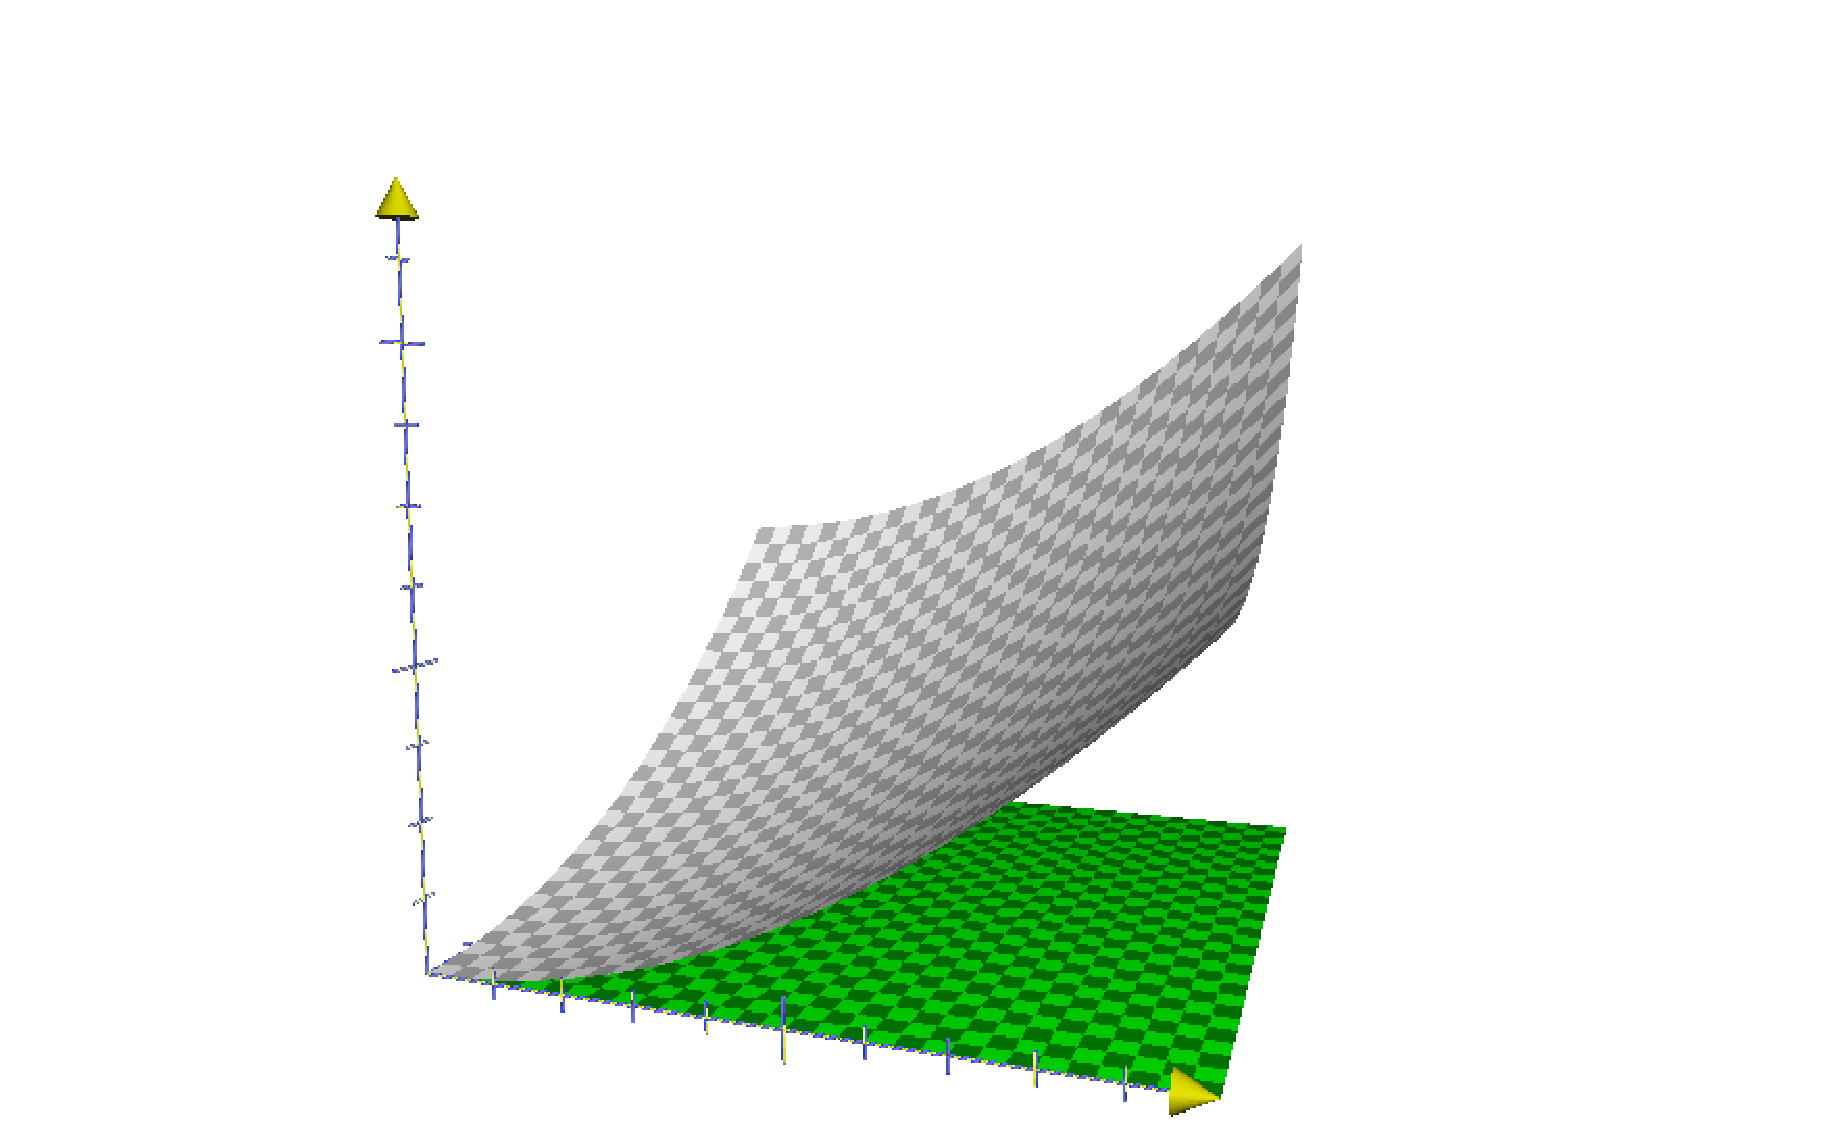
\includegraphics[width=100pt]{03maxmin-on-square.pdf}
  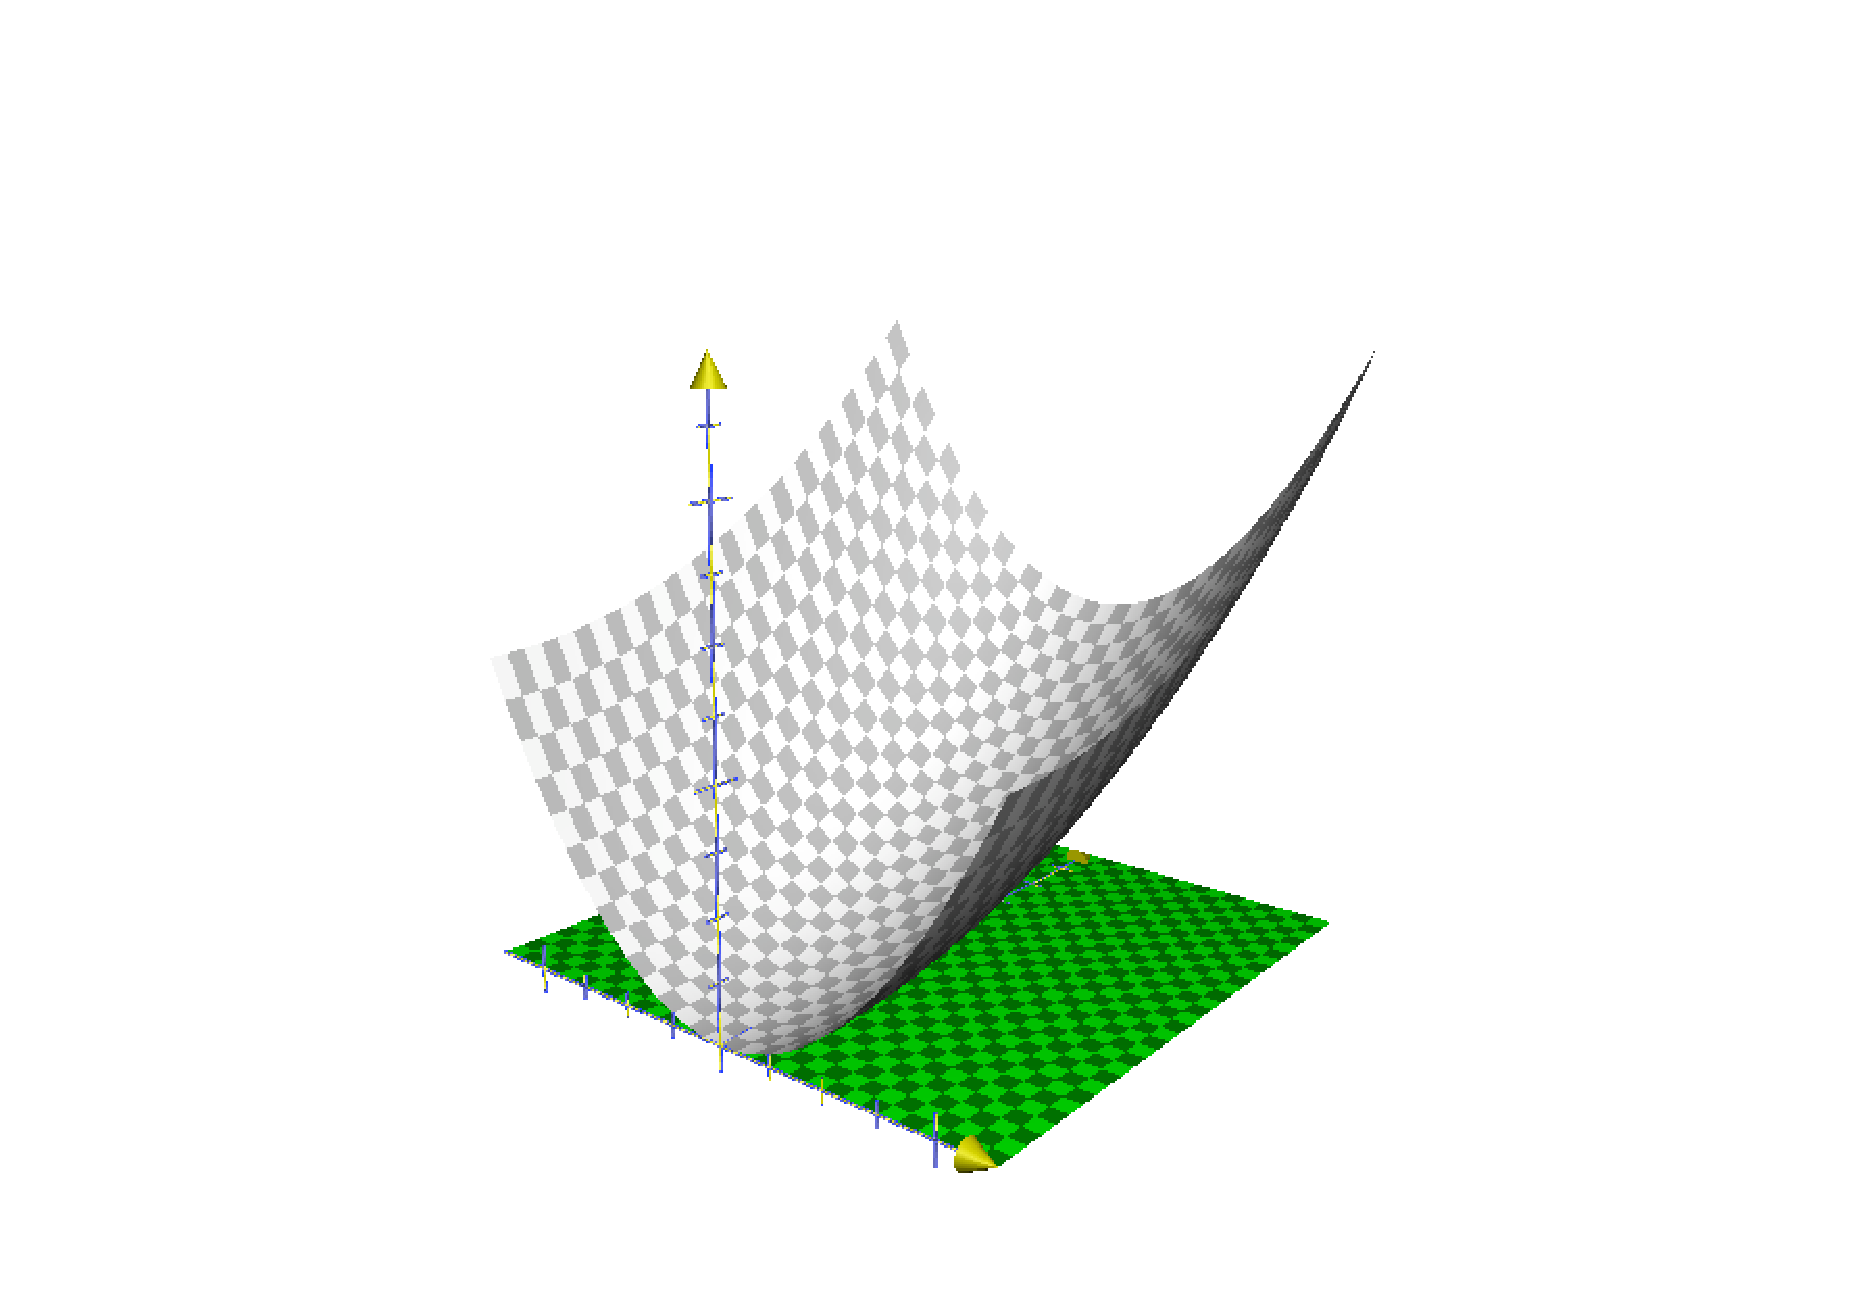
\includegraphics[width=100pt]{03maxmin-on-square2.pdf}
  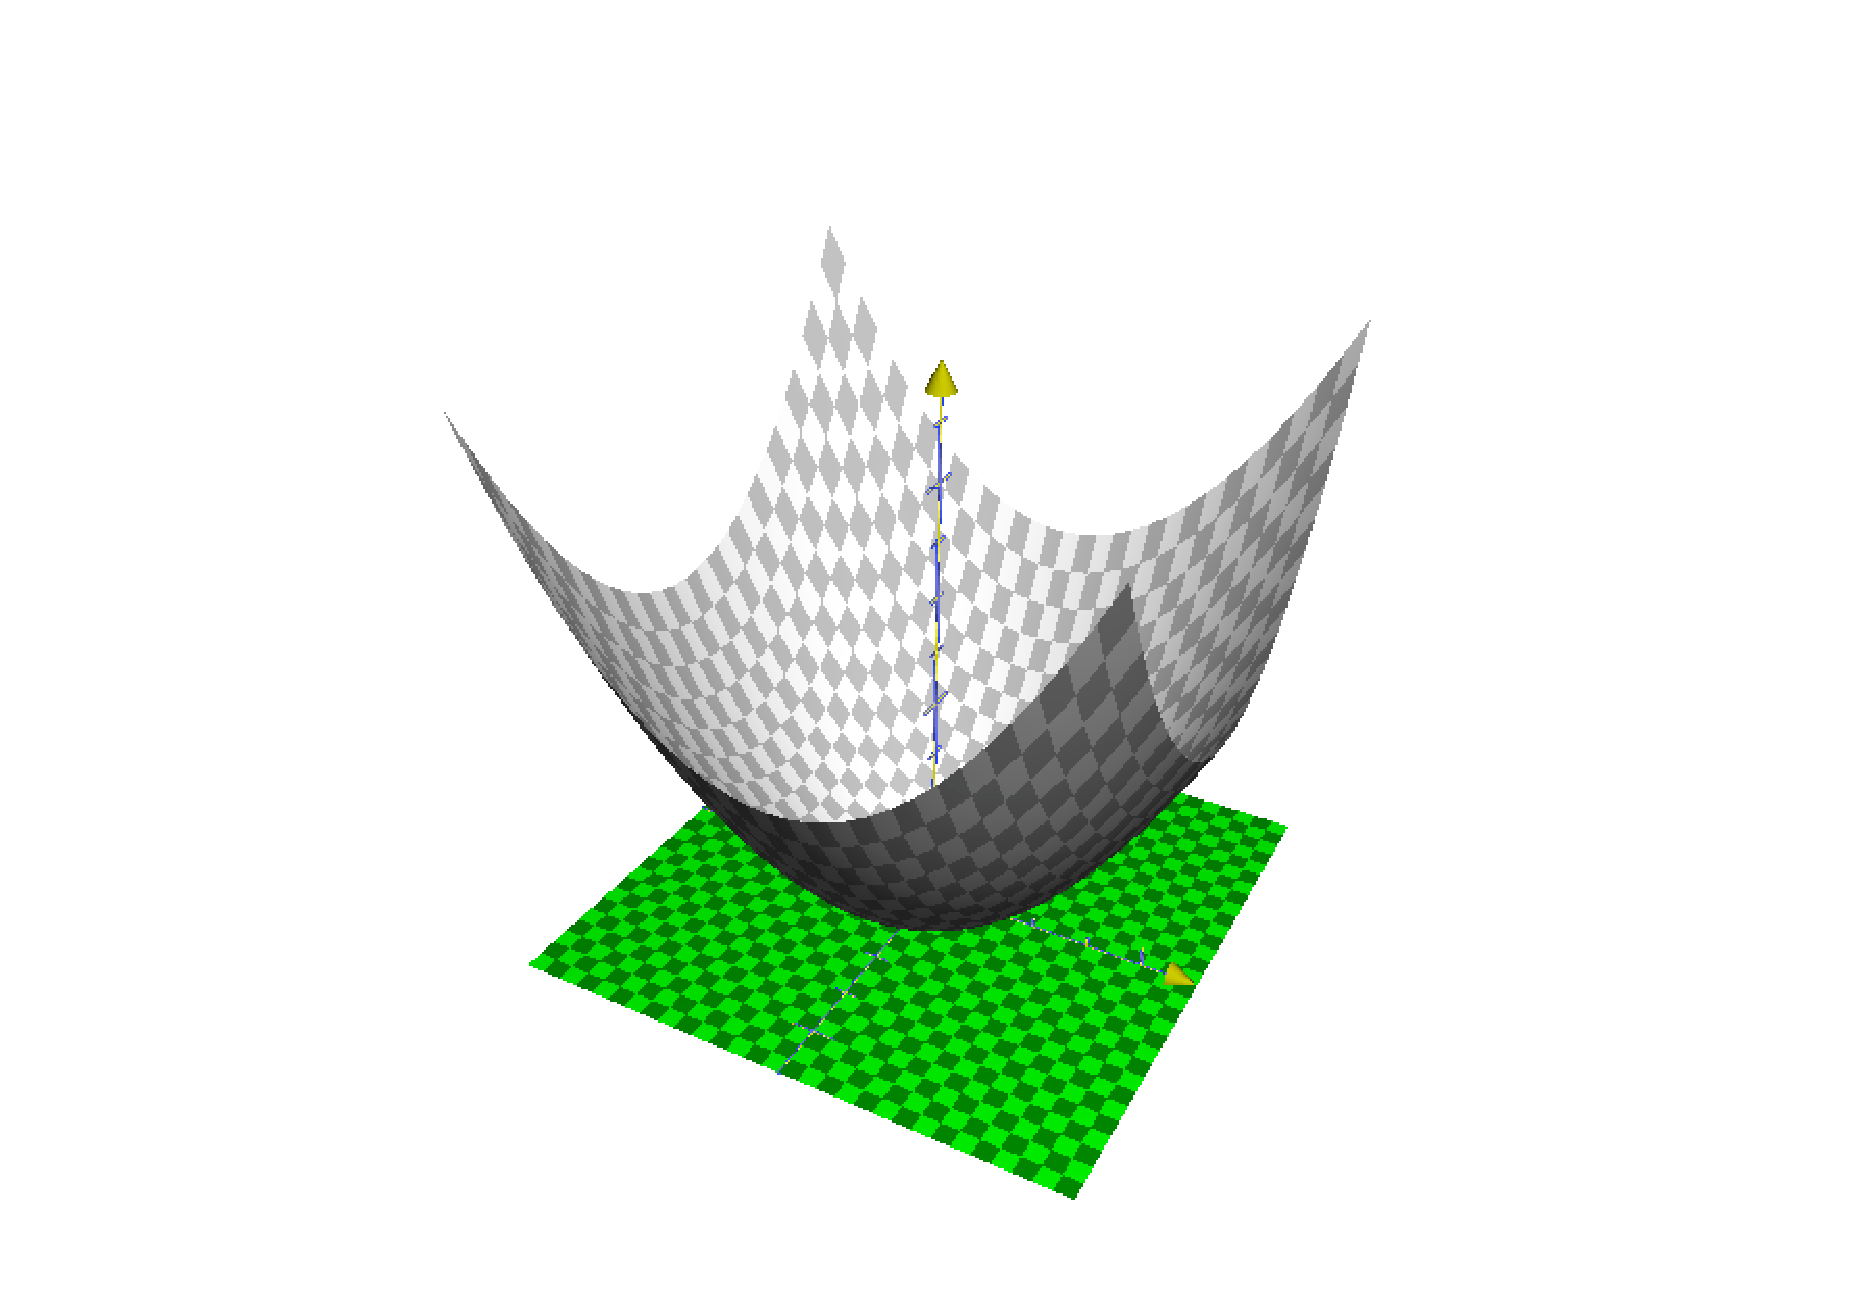
\includegraphics[width=100pt]{03maxmin-on-square3.pdf}
  \caption{The graph of $f(x, y) = x^2+y^2$ from example
    \S~\ref{sec:maxmin-exist-parabolic} on three different rectangles $Q$.
    From left to right:\\
    \null\quad(i) $0\leq x\leq1, 0\leq y\leq1$.
    Both max and min are attained at a corner point of the rectangle.\\
    \null\quad(ii) $0\leq x\leq1, -1\leq y\leq1$. Two maxima, both are attained
    at corner points of the rectangle;
    the minimum is attained at an edge point.\\
    \null\quad(iii) $-1\leq x\leq1, -1\leq y\leq1$, Four maxima, all attained at
    corner points of the rectangle; the minimum is attained at an interior
    point.}
  \label{fig:03maxmin-on-square}
\end{figure}


\label{sec:maxmin-exist-parabolic} 
This function is continuous, and the square $Q = \{(x, y) : 0\leq x\leq1, 0\leq
y\leq1\}$ is bounded, and it contains all boundary points (the edges of the
square).  Therefore Theorem~\ref{thm:maxmin-exist} tells us that $f$ attains
both its highest and lowest values somewhere in the square.  The theorem does
not say where these max/min points are, but in this example they are easy to
find.  The function $f(x, y) = x^2+y^2 $ is at its smallest when both $x=0$ and
$y=0$, i.e.\ at the bottom-left corner of the square.  And $f(x,y)$ is at its
largest when $x$ and $y$ are both as large as they can be, i.e.~when $x=1$ and
$y=1$.  This happens at the top-right corner of the square.

Note that the boundary of the rectangle $Q$ has two different kinds of points:
it has four corner points, and then all the other points that lie on the edges.

If we change the rectangle $Q$ then the minimum can appear at a corner point, a
point on an edge, or in an interior point.  See
Figure~\ref{fig:03maxmin-on-square}.



\subsection{A fishy example}

\label{sec:cubic-maxmin-exist} 
Consider the function $f(x, y) = x^2-x^3-y^2$.  Its zero set is the curve $y^2 =
x^2-x^3$, which is shaped like the letter $\alpha$, or like a fish -- see
Figure~\ref{fig:03maxmin-exist-in-fish}.  The function is positive on the tail
($D_1$) and also on the body ($D_2$) of the fish, it vanishes on the curve that
traces out the fish, and $f$ is negative elsewhere.

We assume that both regions $D_1$ and $D_2$ are closed, which means that we
assume that they include their boundary points. See
Figure~\ref{fig:03maxmin-exist-in-fish} below.

Theorem~\ref{thm:maxmin-exist} does not apply to the region $D_1$ because $D_1$
is not bounded (it contains the whole negative $x$-axis).  But the region $D_2$
is bounded, and our function $f$ is continuous, so
Theorem~\ref{thm:maxmin-exist} does apply to $D_2$.  The theorem tells us that
the function $f$ has a maximal value and a minimal value somewhere in $D_2$.  In
the interior of $D_2$ the function is strictly positive, and at the boundary
points of $D_2$ we have $f=0$.  Therefore each boundary point is a minimum point
of $f$ on $D_2$.  The point(s) in $D_2$ where $f$ attains its highest value must
be somewhere in the interior of $D_2$.  In the next section we will see how to
find it (and how to check that in this case there really only is \emph{one} such
point.)

\begin{figure}[ht]
  \centering
  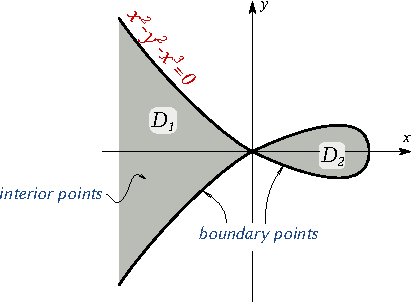
\includegraphics{03maxminexistence.pdf}\hfill
  \includegraphics[width=0.3\textwidth]{03maxmin-cubic.pdf}
  
  \caption{ \textbf{Left: } The region where $f(x, y) = x^2-x^3-y^2$ is positive
    consists of two parts, one bounded ($D_2$), and the other unbounded ($D_1$).
    Theorem~\ref{thm:maxmin-exist} does not apply to the unbounded region, but
    it does apply to the bounded region $D_2$. In that region $f$ must attain a
    maximum and also a minimum.  Since $f=0$ on the boundary of the region
    $D_2$, and $f>0$ in the interior, $f$ achieves its lowest value in $D_2$
    everywhere on the boundary of $D_2$ and its highest value somewhere in the
    interior.  Theorem~\ref{thm:maxmin-exist} does not tell us how to find that
    interior point, and allows for the possibility that there might be
    more interior maxima, as well as a few interior (local) minima.\\
    \null\qquad \textbf{Right: } The graph of the function $z=x^2-y^2-x^3$.}
  \label{fig:03maxmin-exist-in-fish}
\end{figure}



\section{Problems}    
\begin{multicols}{2}
\problemfont 

\problem Suppose you want to find the \emph{maximal value} of $f(x, y) =  
x^2-x^3-y^2$ over all possible $(x,y)$ with $x\geq 0$ (and no restriction
on $y$ -- this region is called the \textit{right half plane}).

\subprob Explain why you should always choose $y=0$ in order to 
maximize this particular function $f(x, y)$.
\answer If $y\neq0$ then you can increase $x^2-x^3-y^2$ by setting $y=0$.  
To put it differently, no matter what you choose for $y$, you always have
\[
  f(x, y) = x^2-x^3-y^2 \leq x^2-x^3  =  f(x, 0).
\]
\endanswer

\subprob Use your answer to part \textbf{(a)} to find the point $(x, y)$ that 
maximizes $f(x,y)$ over the right half plane.
\answer 
The maximum has to appear on the $x$ axis, so the question is
\textit{which $x\geq0$ maximizes $f(x, 0) = x^2-x^3$?}

This is a Math~221 question.  The answer is at $x=2/3$.
\endanswer

\subprob Does our function $f(x,y)$ have a maximal value if $(x,y)$ can be 
any point in the plane?  (hint: what is $f(-1000, 0)$?)
\answer  
No, $\lim_{x\to-\infty} f(x, y) = +\infty$, so $f$ has no largest value.
\endanswer

\problem Suppose that $D$ is a bounded and closed region in the plane (you should draw one: any region will do as long as you include the boundary points).

Where does the function $f(x, y)=x$ attain its maximum in the region that you drew?  Can $f$ attain its maximum at an interior point of the region?

What about minima?

\problem Draw the region
\[
R=\left\{ (x,y) : y^2\leq 4(x^3-x^4)  \right\}.
\]
Find the largest and smallest values that the function
$f(x, y) = x$ can have on this region.  

(Hint: where is $4(x^3-x^4) = 4x^3(1-x)$ positive? The region looks like an Onion).
\answer  
\begin{picture} (120.000000,133.111111)(0,0)
    \put(0.0, 0.0){\includegraphics{03onion.pdf}}
        \put(101.33,  68.56){\sffamily\itshape \makebox[0pt][l]{$1$}}
    \put( 82.94, 116.14){\sffamily\itshape \makebox[0pt][c]{$(\frac34, \frac38\sqrt3)$}}
    \put( 82.94,  11.98){\sffamily\itshape \makebox[0pt][c]{$(\frac34, -\frac38\sqrt3)$}}

\end{picture}
%

The quantity $4(x^3-x^4) = 4x^3(1-x)$ is negative when $x<0$ or
$x>1$, so the region is confined to the vertical strip $0\leq x \leq
1$.  Within this strip $R$ is comprised of those points which satisfy
$-\sqrt{4(x^3-x^4)} \leq y \leq +\sqrt{4(x^3-x^4)}$.  The largest
$x$ value is attained at the point with $x=1$, where $y=0$, so, at the
point $(1,0)$.  The smallest $x$ value is attained at the point
$(0,0)$.   The largest $y$ value is attained at the point where
$y^2 = 4x^3-4x^4$ is maximal.  This happens when $x=\frac 34$, and the
largest $y$ value is therefore $\sqrt{4[(3/4)^3-(3/4)^4]} = \frac
38\sqrt{3}$.  The smallest $y$ value also occurs at $x=\frac 34$ and
is given by $y = -\frac 38 \sqrt 3$.
\endanswer

\noproblemfont
\end{multicols}

\section{Critical points}
For functions $y=f(x), a\leq x\leq b$, of one variable the standard way of finding minima (and maxima) is to look for them in two different places: either the minimum is attained at one of the end points $x=a$ or $x=b$ of the interval, or else the minimum is attained at an interior point.  At an interior minimum one has $f'(x) = 0$, so they can be found by solving the equation $f'(x) = 0$.  The same approach works for functions of two or more variables.  The basic fact that tells us that this is so, is the following theorem.

\subsection{Definition (critical point)} \itshape%
A critical point of a function $z=f(x,y)$ of two variables is a point $(a,b)$ at which $\nab f(a,b) = 0$, i.e.~at which
\[
f_x(a,b) = 0 \text{ and } f_y(a,b) = 0.
\]
\upshape

At a critical point of a function the tangent plane to the graph is horizontal.

\subsection{Theorem.  Local extrema are critical points}

\label{sec:extrema-are-critical} 
\itshape If a function $z=f(x,y)$ defined on a domain $D$ has a local minimum or local maximum at an interior point $(a,b)$ then one has
\[
\frac{\pd f}{\pd x}(a,b)=0, \text{ and } \frac{\pd f}{\pd y}(a,b) = 0.
\]
\upshape
\subsubsection*{Picture proof} (See Figure~\ref{fig:max-are-critical-picture-proof}.)  If $f$ has a local maximum at an interior point $(a,b)$ then $f(x, y) \leq f(a, b)$ for all $(x,y)$ close to $(a,b)$.  This means that a small piece of the graph of $f$ near its local maximum at $(a,b,f(a,b))$ lies below the plane $z=f(a,b)$.  This plane must therefore be the tangent plane to the graph of $f$.  Being horizontal, its slopes are zero, and these slopes are exactly the partial derivatives of $f$ at $(a,b)$.

\subsubsection*{Frozen variable proof}
Suppose $f$ has a local maximum at an interior point $(a,b)$ of the domain $D$.  Then we can freeze the $y$-variable at the value $y=b$ and consider the function of one variable $g(x) = f(x,b)$.  This function has a maximum at $x=a$, so by first semester calculus we know that $g'(x) = 0$.  By definition $g'(a) = f_x(x, b)$, so we conclude that $f_x(a,b) = 0$.

By freezing $x$ instead of $y$ we find that $f_y(a,b)=0$ also must hold.

The same arguments apply in the case of a local minimum.
\begin{figure}[htb]
  \centering

  \includegraphics{02localmax.pdf}
  \caption{\textbf{Theorem~\ref{sec:extrema-are-critical}: } at a local maximum the tangent plane to the graph is horizontal.  The partial derivatives w.r.t.\ both $x$ and $y$ vanish, and in fact, the derivative along \emph{any} path through $(a,b)$ vanishes.  To see a picture of a local minimum turn the page upside down.}
  \label{fig:max-are-critical-picture-proof}
\end{figure}

\subsection{Three typical critical points}

\label{sec:criticalpoint-examples} 
Let's find the critical points of the following three functions:
\[
f(x, y) = x^2+y^2, \quad g(x, y) = x^2-y^2, \quad h(x, y) = -x^2-y^2.
\]
\subsubsection*{$\blacktriangleright f(x, y) = x^2+y^2$}
Computing the partial derivatives we find for the first function
\[
\pdd fx = 2x, \quad \pdd fy = 2y.
\]
If $(x,y)$ is a critical point of $f$ then $x$ and $y$ must satisfy the
equations $f_x(x, y) = 0$ and $f_y(x, y) = 0$, in this case, $2x=0$ and $2y=0$.
So we see that $f$ has exactly one critical point, namely the origin $(x,y) =
(0,0)$.

\textit{Is this critical point perhaps a minimum or a maximum?}  Since squares
can never be negative, $f(x,y) = x^2+y^2$ is always non-negative, and it is at
its smallest when both terms $x^2$ and $y^2$ vanish, i.e.~when $x=y=0$.  So
$f(x, y)$ has a global minimum at the origin.

\subsubsection*{$\blacktriangleright h(x, y) = -x^2-y^2$. } 
This function is just $-f(x,y)$, and without looking at its derivatives we can
tell that it has a global maximum at the origin (because $f(x,y)$ has a global
minimum there).  The derivatives are
\[
\pdd hx = -2x, \quad \pdd hy = -2y
\]
so that the origin is the only critical point of this function.

\begin{figure}[htb]
  \centering
  \includegraphics{02threecriticalpoints.pdf}
  \caption{The three most common kinds of critical point.  See the examples in
    \S\ref{sec:criticalpoint-examples} and also the second derivative test in
    \S\ref{sec:second-deriv-test}.}
  \label{fig:most-common-crpts}
\end{figure}

\subsubsection*{$\blacktriangleright g(x, y) = x^2-y^2$. } 
The derivatives of $g$ are
\[
\pdd gx = 2x, \quad \pdd gy = -2y,
\]
so, once again, the origin is the only critical point.  But, unlike the previous
two functions, $g$ has neither a maximum nor a minimum at the origin.  We can
see this by first looking at what $g$ does on the $x$-axis, and then what $g$
does on the $y$-axis:

On the $x$-axis we have $g(x, 0) = +x^2$, so $g$ has a \emph{minimum} at the
origin.

On the $y$-axis we have $g(0,y) = -y^2$, so $g$ has a \emph{maximum} at the
origin.

So arbitrarily close to the origin we can find points $(x,y)$ where $g(x,y)$ is
larger than $g(0,0)$, and we can find other points where $g(x,y)$ is smaller
than $g(0,0)$.  Therefore $g$ does not have a local maximum or a local minimum
at the origin.

Figure~\ref{fig:most-common-crpts} shows the three cases we have just discussed.


\subsection{Critical points in the fishy example}

\label{sec:critical-fish} 
\textit{What are the critical points of the function $f(x, y) = x^2-x^3-y^2$
  from \S \ref{sec:cubic-maxmin-exist}?}

We compute the partial derivatives of the function
\[
\pdd fx = 2x-3x^2 = (2-3x)x,\qquad \pdd fy = -2y.
\]
The equation $f_y=0$ implies that $y=0$, while $f_x=0$ implies $x=0$ or
$x=\frac{2} {3}$.  Therefore $f$ has two critical points: one at the origin
$(0,0)$, and the other at $(\frac23,0)$.

\marginpar{\includegraphics[width=0.25\textwidth] {03maxminexistence.pdf}}

In this example we could have already predicted from the shape of the zero set
of $f$ that $f$ has at least two critical points -- we don't need to compute the
derivatives of $f$ for that.  Namely, the zero set of $f$ is a curve that
crosses itself at the origin, so the Implicit Function
Theorem~\ref{thm:01implicit-function} (chapter 2) cannot hold at the origin, and
hence $f_x=f_y=0$ there.  And in \S~\ref{sec:cubic-maxmin-exist} we argued that
the function $f$ must have a local maximum somewhere in the region $D_2$
(Figure~\ref{fig:03maxmin-exist-in-fish}), so $f$ must have at least two
critical points.  On the other hand, by computing the critical points we have
found that there is only one local maximum in the region $D_2$.


\subsection{Another example -- find the critical points of $f(x,y) =x-x^3-xy^2$}

\subsubsection*{Solution: } The derivatives of our function are
\[
\pdd fx = 1-3x^2-y^2,\qquad \pdd fy = -2xy.
\]
The critical points are therefore the solutions of the equations
\[
1-3x^2-y^2=0,\qquad -2xy=0.
\]
This is a system of two equations, with two unknowns (that always happens when
we look for critical points, since we are looking for solutions of $f_x(x,y) =
0$, $f_y(x,y)=0$.)  The second equation, $-2xy=0$, implies that either $x=0$ or
$y=0$ (or both).  We have to treat these two cases separately:
\begin{quote}
  \begin{trivlist}
  \item [\bf The case $x=0$. ] If $x=0$ then we only have the first equation
    left, which tells us $1-y^2=0$, i.e.\ $y=\pm1$.  We find two critical points
    with $x=0$, namely, $(0,1)$ and $(0,-1)$.
  \item [\bf The other case, $x\neq0$. ] If $x\neq0$, then the second equation
    ($-2xy=0$) implies $y=0$.  Substitute this in the first equation and we find
    $1-3x^2=0$, i.e.\ $x=\pm\frac{1} {3}\sqrt{3}$, so that we have two critical
    points with $x\neq0$, namely, $(-\frac13\sqrt3, 0)$ and $(\frac13\sqrt3,
    0)$.
  \end{trivlist}
\end{quote}

\begin{figure}[h]
  \centering
  \includegraphics{03example-criticalpoints.pdf}
  \caption{The zero set and signs of the function $f(x,y) =x-x^3-xy^2$.}
  \label{fig:circle-and-line-zero-set-example}
\end{figure}


The conclusion is that this function has four critical points, two on the
$x$-axis, and two on the $y$-axis.  Without looking into this in any further
detail we cannot tell if any of these points are local maxima or minima.  In
general the second derivative test (to be explained in
\S~\ref{sec:second-deriv-test}) will provide this information.  For this example
a look at the zero set of $f$ also helps us figure out what kind of critical
points we have found.  Since $f$ factors as
\[
f(x, y) = x\cdot (1-x^2-y^2),
\]
we see that its zero set consists of the line $x=0$ and the unit circle
$x^2+y^2=1$.  In the above picture $f>0$ in the grey region, and $f<0$ in the
white area.  Consider the right half of the unit disc.  The function is positive
in the interior, and zero on the boundary of this region.  Just as in the
``fishy example'' of \S~\ref{sec:cubic-maxmin-exist}, we have another case where
the maximum of the function must be attained at one or more interior points of
the right half of the unit disc.  According to our computation $f$ only has
\textit{one} critical point in the right half circle, and therefore this point
must be a local maximum of the function.  Conclusion: $D=(\frac13\sqrt3,0)$ is a
local maximum.

In the same spirit you can argue that $f$ has a local minimum at $C$.

The other two points $A,B$ are neither local maxima nor minima, since
\textit{arbitrarily close to $A$ or $B$} there are both points $(x,y)$ with
$f(x,y)$ positive, and points with $f(x,y)$ negative.  The points $A$ and $B$
turn out to be ``saddle points'' (see \S\ref{sec:second-deriv-test} on the
second derivative test.)

\section{When there are more than two variables}
The whole discussion so far has been about functions of two variables.
Fortunately, not much changes when you have more variables.  The concepts
\textit{local minimum} and \textit{local maximum} are defined in the same way,
and it turns out that any \textit{interior local maximum or minimum must be a
  critical point of the function}.  Here, by definition, a critical point of a
function $w=f(x_1, \ldots, x_n)$ of $n$ variables is a solution of the equations
\[
\left\{
  \begin{gathered}
    \pdd f{x_1} (x_1, \cdots, x_n) =0\\
    \pdd f{x_2} (x_1, \cdots, x_n) =0\\
    \vdots\\
    \pdd f{x_n} (x_1, \cdots, x_n) =0.
  \end{gathered}
\right.
\]
Observe that there are $n$ equations, and that there are also $n$ unknowns
($x_1$, \ldots, $x_n$) so that we should \textit{in principle} be able to solve
these equations.  In practice the system of equations we get can be very easy,
difficult, or simply impossible to solve.

\newpage
\section{Problems}  
\begin{multicols}{2}
\problemfont
\problem\label{prb:find-critical-points}  
Find all critical points of the following functions.  Try to classify
them into local/global maxima/minima, saddles, or other kind of
critical points.  (Write clear solutions.  You will need your
solutions later in problem \ref{prb:lots-of-2nd-deriv-tests}.)

\subprob $f(x,y)=x^2+4y^2-2x+8y-1$
%
\answer 
$f_x = 2x-2$, $f_y = 8y+8$, $f_{xx} = 2$, $f_{xy}=0$, $f_{yy}=8$.

There is exactly one critical point, at $(x, y) = (1,-1)$.

The 2nd order Taylor expansion at this point is 
\[
f(1+\Delta x, -1+\Delta y) = 
f(1, -1) + (\Delta x)^2 + 4(\Delta y)^2 +\cdots
\]
The quadratic part is positive definite, therefore $f$ has a
\emph{local minimum} at $(1, -1)$.
\endanswer

\subprob $f(x,y)=x^2-y^2+6x-10y+2$ 
%
\answer 
$f_x = 2x+6$, $f_y = -2y-10$, $f_{xx} = 2$, $f_{xy}=0$, $f_{yy}=-2$.

There is exactly one critical point, at $(x, y) = (-3,-5)$.

The 2nd order Taylor expansion at this point is 
\begin{align*}
  f(-3+\Delta x, -5+\Delta y)
  &= f(-3, -5) + (\Delta x)^2 - (\Delta y)^2 +\cdots \\
  &= f(-3, -5) +\bigl(\Delta x-\Delta y\bigr)\bigl(\Delta x +\Delta
  y\bigr)+\cdots
\end{align*}
The quadratic part factors, therefore $f$ has a
\emph{saddle point} at $(-3, -5)$.  The level set near the critical
point consists of two crossing curves whose tangents are given by the
equations $\Delta x=\Delta y$ and $\Delta x=-\Delta y$.  Since
$\Delta x=x-a=x+3$ and $\Delta y = y-b = y+5$, the two tangent lines
have equations $x+3 = y+5$ and $x+3 = -(y+5)$.
\marginpar{\footnotesize\sffamily
\includegraphics{03answers001.pdf}
\\
Critical point and level set near the critical point.
}%

\endanswer

\subprob $f(x,y)=x^2+4xy+y^2-6y+1$ 
\label{prb:find-cpt-01}
\answer 
$f_x = 2x+4y$, $f_y = 4x+2y-6$, $f_{xx} = 2$, $f_{xy}=4$, $f_{yy}=2$.
There is one critical point: $(x,y) = (2, -1)$.

The 2nd order Taylor expansion at this point is 
\begin{align*}
f(2+\Delta x, -1+\Delta y)
&= f(2, -1) + (\Delta x)^2 + 4 \Delta x \Delta x
            + (\Delta y)^2 +\cdots\\
&= f(2, -1) + \bigl(\Delta x+2\Delta y\bigr)^{2}
            - 3(\Delta y)^2+\cdots\\
&= f(2, -1) + \bigl(\Delta x+(2+\surd3)\Delta y\bigr)
              \bigl(\Delta x+(2-\surd3)\Delta y\bigr)
            +\cdots
\end{align*}
\marginpar{\footnotesize\sffamily
\includegraphics{03answers002.pdf}
\\
Critical point and level set near the critical point.
}%
The quadratic part factors, therefore $f$ has a
\emph{saddle point} at $(2, -1)$.  The level set near the critical
point consists of two crossing curves whose tangents are given by the
equations $\Delta x=-(2+\surd 3)\Delta y$ and $\Delta x=-(2-\surd
3)\Delta y$.  Since $\Delta x=x-a=x-2$ and $\Delta y = y-b = y+1$, the
two tangent lines have equations $x-2 = -(2+\surd3)(y+1)$ and
$x-2 = -(2-\surd3)(y+1)$.
\endanswer

\subprob  $f(x,y)=$\\
\null\hfill$x^2-xy+2y^2-5x+6y-9$ 
\label{prb:find-cpt-02}
\answer 
$f_x = 2x-y-5$, $f_y = -x+4y+6$, $f_{xx} = 2$, $f_{xy}=-1$, $f_{yy}=4$.

There is again one critical point: $x=2$, $y=-1$.

The 2nd order Taylor expansion at this point is 
\begin{align*}
f(2+\Delta x, -1+\Delta y)
&= f(2, -1) + (\Delta x)^2 - \Delta x \Delta x
            + 2(\Delta y)^2 +\cdots\\
&= f(2, -1) + \bigl(\Delta x-\tfrac12\Delta y\bigr)^{2}
            +\tfrac74(\Delta y)^2+\cdots
\end{align*}
The second order part of the Taylor expansion is positive, so
$(2, -1)$ is a \emph{local minimum}.

\endanswer

\subprob $f(x,y) = y^2-18 x^2+x^4$ 
\answer   
$f_x = -36x+4x^3$, $f_y = 2y$, $f_{xx} = -36+12x^2$, $f_{xy}=0$,
$f_{yy}=2$.

The equation $f_x=0$ has three solutions, $x=0$ and $x=\pm3$.
The equation $f_y=0$ has only one solution $y=0$.
Therefore there are three critical points, the origin and the points
$(\pm 3,0)$.

The taylor expansions at these points are
\begin{align*}
    f(\Delta x, \Delta y) 
    &= f(0,0) -18 (\Delta x)^2 + (\Delta y)^2 + \cdots \\
    &= f(0,0) + \bigl(\Delta y-\sqrt{18} x\bigr)\bigl(\Delta y+\sqrt{18} x\bigr)
              + \cdots \\
    f(3+\Delta x, \Delta y) 
    &= f(3,0) +36 (\Delta x)^2 + (\Delta y)^2 + \cdots \\
    f(-3+\Delta x, \Delta y) 
    &= f(-3,0) +36 (\Delta x)^2 + (\Delta y)^2 + \cdots 
\end{align*}
The second order terms in the Taylor expansions at $(3,0)$ and at
$(-3,0)$ are both positive for all $\Delta x$ and $\Delta y$, so both
points $(\pm3, 0)$ are local minima.  The second order part of the
expansion at the origin factors and hence the origin is a saddle
point.  The tangents to the zeroset at the origin are the lines
$\Delta y = \pm \sqrt{18}\Delta x = \pm 3\sqrt2 \Delta x$.  Since here
$\Delta x = \text{``}x-a\text{''} = x$, and $\Delta y = y$, the
tangents are the lines through the origin given by $y=\pm 3\sqrt2 x$.

You can try to draw the zeroset of this function and analyze it in the
same way as the ``fishy example'' in \ref{sec:critical-fish}.  The
zeroset of $f$ consists of the graphs of $y = \pm \sqrt{18x^2-x^4} =
\pm |x|\sqrt{18-x^2}$.
It looks like a squashed ``$\infty$'' or a butterfly (you decide.)
\marginpar{\footnotesize\sffamily
\includegraphics{03answers003.pdf}
\\
Critical points and zero set.
}
\endanswer
\subprob $f(x,y) = y^4-4y^2-18 x^2+x^4$ 
%
\answer    
There are nine critical points. Four global minima at $(\pm 3,
\pm\sqrt{3})$, four saddle points at $(0,\pm\sqrt{3})$ and $(\pm3,0)$
respectively, and finally, a local but not global maximum at the
origin.
\endanswer

\subprob $f(x,y)=9+4x-y-2x^2-3y^2$ 
%
\answer critical point at $(1,-1/6)$  
$f_x = 4-4x$, $f_y = -1-6y$, $f_{xx} = -4$, $f_{xy}=0$, $f_{yy}=-6$.

Second order Taylor expansion at the critical point:
\[
f(-1+\Delta x, -\tfrac16+\Delta y) = f(1, -\tfrac16)
-2(\Delta x)^2-3(\Delta y)^2 + \cdots
\]
The second order terms are always negative so $(1, -\tfrac16)$ is a
local maximum.
\endanswer

\subprob $f(x,y)=xy(4-x-2y)$ 
%
\answer The derivatives are: 
\[
f_x = 4y-2xy-2y^2,\quad f_y = 4x-x^2-4xy,\quad f_{xx} = -2y,\quad
f_{xy}=4-2x-4y,\quad f_{yy}=-4x.
\]
This function is given in factored form, so without solving the
equations $f_x=0$, $f_y=0$ you can say the following about this
problem.  The zero set consists of the three lines: the $y$-axis
($x=0$), the $x$-axis ($y=0$) and the line with equation $4-x-2y=0$.
It follows that the intersection points $(0,0)$, $(4,0)$, and $(0,2)$
of these lines are saddle points.  Since $f>0$ in the triangle formed
by the three lines this triangle must contain at least one local
maximum.

\begin{center}
  \includegraphics{03answers004.pdf}
\end{center}
To find all critical points solve these equations:
\[
f_x = 4y-2xy-2y^2 = 0 \iff \text{\framebox{$y=0$ or $4-2x-2y=0$}}
\]
and 
\[
f_y = 4x-x^2-4xy=0  \iff \text{\framebox{$x=0$ or $4-x-4y=0$}}
\]
Since both equations $f_x=0$ and $f_y=0$ lead to two possibilities, we
have to consider $2\times 2=4$ cases:
\begin{description}
  \item[$y=0$ \& $x=0$] This tells us the origin is a critical point
  \item[$y=0$ \& $4-x-4y=0$] Solving these equations leads to
    $x=4, y=0$, so $(4,0)$ is a critical point.
  \item[$4-2x-2y=0$ \& $x=0$] Solve and you find that $(0,2)$ is a
    critical point.
  \item[$4-2x-2y=0$ \& $4-x-4y=0$] Solve these equations and you get
    $(x,y) = (\tfrac43, \tfrac23)$.
\end{description}
The first three critical points are the saddle points we predicted.
The fourth critical point must be a local maximum, since there has to
be one in the triangle, and of all the critical points we have found
the others are all saddle points.
\endanswer

\subprob $f(x,y)=x(x-y)(x-1)$ 
\answer
Two saddle points:  $(0,0)$ and $(1,1)$.
\endanswer

\subprob $f(x,y)=(x-y)(xy-4)$ 
%
\answer Two saddle points:  $(2,2)$ and $(-2,-2)$  
%$f_x = <++>$, $f_y = <++>$, $f_{xx} = <++>$, $f_{xy}=<++>$, $f_{yy}=<++>$.
\endanswer

\subprob $f(x,y)=y^2+\cos x$ 
%
%\answer    
%$f_x = <++>$, $f_y = <++>$, $f_{xx} = <++>$, $f_{xy}=<++>$, $f_{yy}=<++>$.
%\endanswer

\subprob $f(x,y)=x^2y-\frac13 y^3$ 
%
\answer The origin. Neither a local max, min, nor saddle.  
The graph of this function is called the ``Monkey Saddle'' as
it accommodates two legs and a tail too.  Draw it in your graphing
program to see this.
\endanswer

\subprob $f(x,y)=(x-y^2)(x-1)$ 
%
\answer    
Zero set is the parabola with equation $x=y^2$, and the line
$x=1$.  They intersect at $(1, \pm1)$, so the function has two saddle
points $(1,1)$ and $(1,-1)$.  The region between the line $x=1$ and
the parabola must contain  local minimum.  It is located at
$(\frac12, 0)$.
\endanswer

\subprob $f(x,y)=(x-y)(xy-4)$ 
%
\answer Two saddle points : $(2,2)$ and $(-2,-2)$.  
Yes, this problem appeared twice.
\endanswer

\subprob $f(x,y) = x^2$ 
%
\answer  All points on the $y$-axis are critical points.  They are all  
global minima, but the second derivative test doesn't tell you so.
\endanswer

\subprob $f(x,y) = x^2y$ 
%
\answer  
All points on the $y$-axis are again critical points.  Those with
$y>0$ are local minima, those with $y<0$ are local maxima, and the
origin is neither.  The second derivative test applies to none of
these points.
\endanswer

\subprob $f(x,y) = \bigl(1-x^2-y^2\bigr)^2$ 
%
\answer  All points on the unit circle are global minima, because the  
function vanishes there, and is positive everywhere else.  The origin
is a local maximum.  The 2nd derivative test applies to the origin,
but not to any of the other critical points.
\endanswer

\subprob $f(x,y) = x^2y$ 
%
\answer  
All points on the $y$-axis are again critical points.  Those with
$y>0$ are local minima, those with $y<0$ are local maxima, and the
origin is neither.  The second derivative test applies to none of
these points.
\endanswer

\problem % about f(x, y) = sin x sin y    

\subprob Draw the zero set of the function $f(x, y) = \sin(x) \sin(y)$.

\subprob Where is the function $f$ positive?  Find as many critical points as
you can without computing $f_x$ or $f_y$.

\subprob Find all critical points of $f(x, y)$.  Which are local minima or local
maxima?

\problem Find the critical points of the function 
\[
f(x, y, z) = x^2 + y^2 + z^2 - 2x + 4y -2.
\]

\problem Draw the zero set and find the critical points of the functions
\[
f(x, y, z) = x^2+y^2 - z^2
\]
and
\[
g(x, y, z) = x^2-y^2 - z^2
\]

\problem If we have three points $A$,  $B$, and $C$ in the plane, \textit{which point is closest to all three of them?}  The answer depends on what we mean by ``closest to all three points.''  The following problem gives us one interpretation of this general question.

Consider the three points $(1,4)$, $(5,2)$, and $(3,-2)$ in the plane.  The function 
\begin{multline*}
f(x, y, z) = \\
(x-1)^2+(y-4)^2+\\
(x-5)^2+(y-2)^2+\\
(x-3)^2+(y+2)^2
\end{multline*}
is the sum of the squares of the distances from point $(x,y)$ to the
three points.  

\subprob Assuming that there is a global minimum, find $x$ and $y$ so that $f(x,y)$  is minimized. 
\answer  $(3,4/3)$  
\endanswer

\subprob (For discussion)  Does $f(x,y)$ have a global minimum?  How can we be sure
that the point we found in part \textbf{(a)} is not actually a maximum or some other
critical point?
%
\subprob Given the three points $(a, b)$, $(c, d)$, and $(e, f)$,  
let $f(x, y)$ be the sum of the squares of the distances from point
$(x,y)$ to the three points.  Find $x$ and $y$ so that this quantity is
minimized. 
\answer
$x= (a+c+e)/3$, $y=(b+d+f)/3$.  
\endanswer

\problem Suppose that a function $f(x, y)$ factors, i.e.~we can write it as the
product of two other differentiable functions, $f(x, y) = g(x, y)h(x, y)$.

\textit{Prove: if a point $(a, b)$ lies in the zero set of $g$ and also in the
zero set of $h$, then $(a,b)$ is a critical point of $f$.}

\noindent%
Hint: compute the partial derivatives of $f$ by applying the product rule to $f=g\cdot h$.
\answer
You have to show that $f_x(a, b) = f_y(a, b) = 0$.
By the product rule $f_x(a, b) = g_x(a, b)h(a, b) + g(a, b) h_x(a,
b)$.  Since both $g(a, b) = 0$ and $h(a, b) = 0$, it follows that
$f_x(a, b) = 0$.   The same reasoning applies to $f_y(a, b)$.
\endanswer

\problem Find the critical points of the functions 

\subprob $  f(x, y, z) = x^2 + y^2 + z^2 - 2x + 4y -2$ 

\subprob $  f(x, y, z) = x^4 + y^2 + z^2 - 2xz + 4y$ \\

\subprob $  f(x, y, z) = xyze^{-x-y-z}$ 

\subprob $f(x,y,z) = x^2+y^2+z^2 - 2xyz$ 



\noproblemfont
\end{multicols}
\section{A Minimization Problem: Linear Regression}

\label{sec:linear-regression}

Suppose we are measuring two quantities $x$ and $y$ in some experiment, and
suppose that we expect that there is a linear relation of the form $y=ax+b$
between $x$ and $y$.  If we have a set of data points $(x_k, y_k)$ from our
experiment, then what do they tell us about $a$ and $b$?  \emph{Which choice of
  coefficients $a$ and $b$ bests fits our data? } Because of experimental errors
we would not expect our data points to lie on a straight line, but instead, we
expect them to be clustered around a straight line.  We could plot the data
points, get a ruler, and draw a straight line by hand that looks like the best
match -- then we could measure $a,b$ from our drawing.  A more systematic
approach is to first define what we mean by ``best match'' and then find the
line that best matches according to our chosen criterion.

A very common criterion is the least-mean-square-fit.  To describe it, imagine
we have $N$ data points, $(x_1,y_1)$, \dots\, , $(x_N, y_N)$, and consider the
line with coefficients $a$ and $b$.  Most data points $(x_k, y_k)$ will then
probably not lie on the line $y=ax+b$, and one uses
\[
E_k = \tfrac12\bigl(ax_k+b-y_k\bigr)^2
\]
as a measure for the mismatch between the data point $(x_k, y_k)$ and the line
$y=ax+b$ (the factor $\frac12$ makes formulas later on nicer).  Adding all these
errors we get the total ``mean square'' error
\[
E= E_1 + \cdots + E_N.
\]
If we think of all the numbers $x_1, \ldots, x_N, y_1, \ldots, y_N$ as given
constants (after all, we measured them, so we shouldn't change them any
more\footnote{This is called the ``Sushi Principle'': \textit{raw data is better
    than cooked data.}}), then the total error only depends on the coefficients
$a$ and $b$.  It is a measure for how well the line $y=ax+b$ fits our data
points, and the common method of \emph{linear regression} consists in choosing
the coefficients $a$ and $b$ so as to minimize this error $E$.

\begin{figure}[htb]
  \centering \begin{picture} (300.000000,162.461538)(0,0)
    \put(0.0, 0.0){\includegraphics{02linearregression.pdf}}
        \put(241.69, 116.18){\sffamily\itshape \makebox[0pt][l]{\rotatebox{16.699244}{$y=ax+b$}}}
    \put(207.31,  46.02){\sffamily\itshape \makebox[0pt][c]{$(x_k, y_k)$}}
    \put(211.31,  78.94){\sffamily\itshape \makebox[0pt][l]{$\bigl|ax_k+b-y_k\bigr|$}}

\end{picture}

  \caption{Which line best fits a set of data points?}
  \label{fig:linear-regression}
\end{figure}

This leads us to the problem of finding the critical points of the total error
$E$ as a function of $a$ and $b$.  We have to solve
\[
\pdd Ea = 0 \qquad \pdd Eb = 0.
\]
The total error is the sum of the individual errors $E_k(a, b)$ so we get
\[
\pdd Ea = \pdd{E_1}a + \cdots +\pdd {E_N}a, \qquad \pdd Eb = \pdd{E_1}b + \cdots
+\pdd {E_N}b.
\]
The individual errors have the following derivatives:
\[
\pdd{E_k}a = x_k\bigl(ax_k+b-y_k\bigr),\qquad \pdd{E_k}b = ax_k+b-y_k.
\]
Adding all these derivatives then leads to
\begin{align*}
  \pdd Ea &= \sum x_k\bigl(ax_k+b-y_k\bigr) \\
  &= (\tsum x_k^2) a + (\tsum x_k) b - \tsum x_ky_k
\end{align*}
and
\begin{align*}
  \pdd Eb &= \sum \bigl\{ax_k+b-y_k\bigr\} \\
  &= (\tsum x_k) a + N b - \tsum y_k
\end{align*}
Here ``$\sum$'' represents summation over $k=1, \cdots, N$, i.e.\ $\sum x_ky_k =
x_1y_1+\cdots+x_Ny_N$, etc.

If $(a,b)$ is a critical point then $a$ and $b$ must satisfy
\begin{align*}
  (\tsum x_k^2) a + (\tsum x_k) b &= \tsum x_ky_k \\
  (\tsum x_k) a + N b &= \tsum y_k
\end{align*}
These are two linear equations for the two unknowns $a$ and $b$.  Solving them
leads to
\[
a = \frac{N\sum x_ky_k \; - \; \sum x_k \sum y_k} {N\sum x_k^2 - \bigl(\sum
  x_k\bigr)^2}\; ; \qquad b = \frac{-\sum x_k \sum x_ky_k + \sum x_k^2 \sum y_k}
{N\sum x_k^2 - \bigl(\sum x_k\bigr)^2}\; .
\]
These are the standard formulas for the coefficients $a$ and $b$ provided by the
method of linear regression.  Most calculators, and certainly all spreadsheets
(like Excel) have these formulas preprogrammed, so we only have to enter the
data points $(x_k,y_k)$ and ``push the right button'' to get $a$ and $b$.

\section{Problems} 
\begin{multicols}{2}
\problemfont
%\immediate\write\ans{\string\newpage}
\problem  We are given $N$ measurements $x_1$, \ldots, $x_N$  
from some experiment, and, inspired by the Linear Regression example,
we decide to see which number $a$ ``best fits the data.''  We define
the error (or ``measure of misfit'') for each measurement to be
\[
E_k(a) = \tfrac12(a-x_k)^2
\]
and we look for the number $a$ which minimizes the total error
\[
E(a) = E_1(a) + \cdots + E_N(a).
\]
\subprob  Is this a problem about several variable calculus, or about 
one variable calculus?
\answer  
One variable calculus!  There is only one variable, $a$, and we must
solve $E'(a) = 0$.
\endanswer

\subprob Which number $a$ do we find? 
\answer  
$a= (x_1+\cdots+x_N)/N$, i.e.\ the average provides ``the best fit.''
\endanswer

\problem We have a series of data points $(x_k, y_k)$,  
and when we plot them we think we see a convex curve rather than a
straight line.  In fact it looks like a parabola, and so we
set out to find a quadratic function $y=ax^2+bx+c$ that minimizes the
error
\[
E(a,b,c)=E_1+\cdots+E_N,
\]
with
\[
E_k(a, b, c) = \tfrac12\bigl(ax_k^2+bx_k+c - y_k\bigr)^2.
\]
\subprob How many variables are there in this problem? 
\answer Three:  $a$, $b$, and $c$. 
\endanswer
\subprob If $(a, b, c)$ is a critical point of $E(a, b, c)$  
then $a$, $b$, and $c$ satisfy three linear equations.  Find these
equations (don't solve them).
\answer The equations for $(a, b, c)$ are:   
\[
\begin{array}{rlcrlcrlrcl}
    (\tsum x_k^4)&a &+&(\tsum x_k^3)&b &+& (\tsum x_k^2)&c 
    &=& \tsum x_k^2y_k\\[1ex]
    (\tsum x_k^3)&a &+&(\tsum x_k^2)&b &+& (\tsum x_k)&c 
    &=& \tsum x_ky_k\\[1ex]
    (\tsum x_k^2)&a &+&(\tsum x_k)&b &+& N&c &=& \tsum y_k
\end{array}
\]
\endanswer

\problem A measurement in a certain experiment results 
in three numbers $(x, y, z)$.  The point of the experiment is to see
if there is a linear relation of the form $z=ax+by+c$ between the
three measured quantities, and to estimate the coefficients $a, b, c$.

After repeating the experiment $N$ times we have $N$ data points
$(x_k, y_k, z_k)$ ($k=1, \ldots, N$).  We decide to choose $a,b,c$ so
as to minimize the mean square error
\[
E=E_1+\cdots+E_N,
\]
with
\[
E_k(a, b, c) = \tfrac 12 \bigl(ax_k+by_k+c- z_k\bigr)^2.
\]
Which (linear) equations will we get for $a$, $b$, and $c$?
\answer The equations are 
\[
\begin{array}{rlcrlcrlrcl}
    (\tsum x_k^2)&a &+&(\tsum x_ky_k)&b &+& (\tsum x_k)&c 
    &=& \tsum x_kz_k\\[1ex]
    (\tsum x_ky_k)&a &+&(\tsum y_k^2)&b &+& (\tsum y_k)&c 
    &=& \tsum y_kz_k\\[1ex]
    (\tsum x_k)&a &+&(\tsum y_k)&b &+& N&c &=& \tsum z_k
\end{array}
\]
\endanswer
\noproblemfont
\end{multicols}

\section{The Second Derivative Test}    
\label{sec:second-deriv-test}

\subsection{Review of the one-variable second derivative test and Taylor's formula}
For a function $y=f(x)$ of one variable you can tell if a critical
point $a$ is a local maximum or minimum by looking at the sign of the
second derivative $f''(a)$ of the function at that point.  

\begin{figure}[ht]\centering
  \includegraphics{03onevariable-2ndderivtest.pdf}
\end{figure}
If $f''(a)>0$ then the graph of $f$ is curved upwards and $f$ has a local
minimum at $a$; if $f''(a)<0$ then $f$ has a local max.  This section
is about the analogous test for critical points of functions of two
variables.  

One way to understand the second derivative test is to look at the
Taylor expansion of the function $y=f(x)$.  If $x=a$ is a critical
point for $f$, then
\[
f(x) = f(a) + f'(a)(x-a) + \tfrac 12 f''(a)(x-a)^2
+\cdots
\]
Since $a$ is a critical point of $f$ we have $f'(a)=0$, so that the
Taylor expansion reduces to
\begin{equation}\label{eq:one-variable-expansion-at-cpt}
  f(x) = f(a) + \tfrac 12 f''(a)(x-a)^2 +\cdots
\end{equation}
If we ignore the remainder term (the dots), then we find that
\[
f(x) \approx f(a) + \tfrac 12 f''(a)(x-a)^2.
\]
Near the critical point the graph of $y=f(x)$ is a approximately a
parabola. It is curved upwards if $f''(a)>0$, and downwards if
$f''(a)<0$.

To apply the same reasoning to a function of two (or more) variables
we need to know the Taylor expansion of such a function.

\subsection{Taylor's formula for a function of several variables}
\label{sec:Taylor-derived}
The Taylor expansion of a function $z=f(x, y)$ should give us an
approximation of $f(a+\Delta x, b+\Delta y)$ in terms involving powers
of $\Delta x$ and $\Delta y$.  There is a general formula, but here we
only need the second order terms, so we'll derive those and stop
there.

The trick to finding the Taylor expansion is to consider the function
\begin{equation}
  g(t) = f(a+t\Delta x, b+t\Delta y).
\end{equation}
By definition
\[
g(1) = f(a+\Delta x, b+\Delta y)
\]
is the quantity we want to approximate, and $g(0) = f(a, b)$.  Since
$g(t)$ is a function of one variable, we can apply Taylor's formula
from Math~222 to it.  We get:
\begin{equation}\label{eq:03gtaylor}
  g(t) = g(0) + g'(0) t + g''(0)\frac{t^2}{2!} + \cdots
\end{equation}
The dots contain the remainder term, which we will ignore.  Now we set
$t=1$, and we get
\[
g(1) = g(0) + g'(0) + \frac{1}{2} g''(0)+ \cdots
\]
The derivatives of $g$ can be computed with the chain rule:
\begin{align}\label{eq:03-gfirstderiv}
  g'(t)
  &= \frac{d f(a+t\Delta x, b+t \Delta y)}{dt} \\
  &= f_x(a+t\Delta x, b+t \Delta y)\frac{d(a+t\Delta x)}{dt}
  + f(a+t\Delta x, b+t \Delta y)\frac{d(b+t\Delta y)}{dt}\notag \\
  &= f_x(a+t\Delta x, b+t \Delta y)\Delta x + f_y(a+t\Delta x, b+t
  \Delta y) \Delta y.\notag
\end{align}
The second derivative is
\begin{multline}\label{eq:03-gseconderiv}
  g''(t) = f_{xx}(a+t\Delta x, b+t \Delta y)(\Delta x)^2 \\
  + 2f_{xy}(a+t\Delta x, b+t \Delta y) \Delta x\Delta y\\
  + f_{yy}(a+t\Delta x, b+t \Delta y) (\Delta y)^2.
\end{multline}
In computing $g''(t)$ we run into terms involving $f_{xy}$ and terms
with $f_{yx}$.  Because of Clairaut's theorem these are the same, and
combining them leads to the coefficient ``$2$'' in front of $f_{xy}$
above.

Setting $t=0$ in \eqref{eq:03-gfirstderiv} and in
\eqref{eq:03-gseconderiv} gives you expressions for $g'(0)$ and
$g''(0)$, and by substituting these in \eqref{eq:03gtaylor} we get
\emph{the second order Taylor expansion of a function of two
  variables:}
\begin{multline}\label{eq:second-order-taylor}
  f(a+\Delta x, b+\Delta y) = f(a, b)
  + f_x(a, b) \Delta x + f_y(a,b) \Delta y\\
  +\frac{1}{2}\Bigl\{ f_{xx}(a, b)(\Delta x)^2 + 2f_{xy}(a,b)\Delta x
  \Delta y + f_{yy}(a,b)(\Delta y)^2 \Bigr\} +\cdots
\end{multline}
\begin{figure}[ht]
  \centering
  \includegraphics[scale=1.5]{03taylor-dx-dy.pdf}
  \caption{\textbf{$\Delta x$ and $\Delta y$:} Taylor's formula lets us
    approximate a function $z=f(x,y)$ at points $(x,y) = (a+\Delta x, b+\Delta
    y)$ close to $(a,b)$.  The expansion gives us $f(x,y) = f(a+\Delta x,
    b+\Delta y)$ as a function of $\Delta x$ and $\Delta y$.}
\end{figure}
The first three terms are exactly the linear approximation
\eqref{eq:linear-approximation-no-error} of the function that we saw in
Chapter~III, \S~\ref{sec:linear-approximation-no-error}.  The next terms in ~\ref{eq:second-order-taylor} are
\[
\frac{1}{2}f_{xx}(a, b)(\Delta x)^2
+ f_{xy}(a,b)\Delta x \Delta y
+ \frac12 f_{yy}(a,b)(\Delta y)^2.
\]
These terms determine a quadratic form in the variables $\Delta x$ and $\Delta
y$. The quantities $\frac12 f_{xx}(a,b)$, etc.~are the coefficients of the form.


As always, the dots in the expansion \eqref{eq:second-order-taylor} contain the
remainder term.  By carefully including the one-variable Lagrange remainder in
the derivation we can get a formula for the remainder in
\eqref{eq:second-order-taylor}.  We will not do that, but it can be shown that
the remainder is $o\left( (\Delta x)^2 + (\Delta y)^2 \right)$, i.e.\ that it is
small compared to the other terms in the expansion, at least when $\Delta x$ and
$\Delta y$ are small.
% :CONTINUE HERE

\subsection{Example -- compute the Taylor expansion of $f(x, y) = \sin2x\cos y$
  at the point $(\frac16\pi, \frac16\pi)$}
%\marginpar{\dfnt%
%maybe $x^2\ln y	$ is an easier example?}
To find the expansion we need to compute $f, f_x, f_y, f_{xx},
f_{xy},$ and $f_{yy}$ at $(\frac16\pi, \frac16\pi)$.  Here goes:
\[
\begin{aligned}
  f&= \sin 2x \cos y = \tfrac 34 \\
  f_x&=2\cos 2x\cos y = \tfrac12\sqrt{3}\\
  f_y&=-\sin2x \sin y = -\tfrac 14\sqrt3 
\end{aligned}
\qquad
\begin{aligned}
  f_{xx}&=-4\sin2x\cos y = -3 \\
  f_{xy}&=-2\cos 2x\sin y = -\tfrac12 \\
  f_{yy}&=-\sin 2x\cos y = -\tfrac 34.
\end{aligned}
\]
Substituting in the Taylor expansion we get
\begin{align*}
  f\bigl( \tfrac16\pi+\Delta x, &\tfrac16\pi+\Delta y\bigr)\\
  &=
  \tfrac 34 +\tfrac12\sqrt3 \,\Delta x -\tfrac14\sqrt3\,\Delta y
  +\frac12\Bigl\{
  -3(\Delta x)^2 -2\cdot\tfrac12 \Delta x \Delta y - \tfrac34 (\Delta
  y)^2
  \Bigr\} + \cdots\\
  &=\tfrac 34 +\tfrac12\sqrt3 \,\Delta x -\tfrac14\sqrt3\,\Delta y
  -\tfrac32(\Delta x)^2 -\tfrac12 \Delta x \Delta y -\tfrac38(\Delta y)^2
  +\cdots
\end{align*}
Note that the first three terms in the expansion are the linear
approximation of the function:
\[
f\bigl( \tfrac16\pi+\Delta x, \tfrac16\pi+\Delta y\bigr)
= \tfrac 34 +\tfrac12\sqrt3 \, \Delta x -\tfrac14\sqrt3\, \Delta y +\cdots
\]

\subsection{Another example -- the Taylor expansion of $f(x, y) = x^3+y^3-3xy$
  at the point $(1,1)$}
\label{sec:taylor-example-at-minimum}
The function $f(x, y) = x^3+y^3-3xy$ has the
following derivatives at $(1,1)$:
\[
\begin{aligned}
  f & =  x^3+y^3-3xy &= 1 \\
  f_x&= 3x^2 - 3y &= 0 \\
  f_y&= 3y^2-3x &= 0
\end{aligned}\hspace{0.25\textwidth}
\begin{aligned}
  f_{xx} &= 6x &=&\;6 \\ f_{xy} &=-3 &=&-3 \\ f_{yy} &= 6y &=&\;6
\end{aligned}
\]
The first derivatives vanish, so $(1,1)$ is a critical point of $f$.
The second order Taylor expansion of $f$ at $(1,1)$ is
\begin{equation}\label{eq:example-taylor-expansion}
  f(1+\Delta x, 1+\Delta y)
  = 1 + 3(\Delta x)^2 - 3\Delta x \Delta y + 3(\Delta y)^2 +\cdots
\end{equation}
Note that there are not first order terms in this expansion because $(1,1)$ is a critical point -- the coefficients of the first order terms are both zero.

To see what kind of critical point $(1,1)$ is, we have to analyze the second
order, quadratic, terms
\begin{equation}
  3(\Delta x)^2 - 3\Delta x \Delta y + 3(\Delta y)^2.
  \label{eq:example-quadratic-form}
\end{equation}
This expression is a quadratic form in $\Delta x$ and $\Delta y$, and by
completing the square (see Chapter~III, \S~\ref{sec:quadratic-forms}) we
find that
\[
3(\Delta x)^2 - 3\Delta x \Delta y + 3(\Delta y)^2
=3 \Bigl[\bigl(\Delta x - \tfrac 12 \Delta y\bigr)^2
  + \tfrac 34 (\Delta y)^2\Bigr].
\]
In particular, the quadratic terms in the Taylor expansion of $f$ at the
critical point are always positive, no matter what $\Delta x$ and $\Delta
y$ we choose (as long as they are not both zero).  If we are allowed to
ignore the remainder term (the ``$\cdots$''), then this implies that the
function has a local minimum: after all, the Taylor expansion
(\ref{eq:example-taylor-expansion}) says that for small $\Delta x$ and
$\Delta y$ the function value $f(1+\Delta x, 1+\Delta y)$ is 
\[
f(1+\Delta x, 1+\Delta y) \approx 
f(1, 1) + 3 \bigl(\Delta x - \tfrac 12 \Delta y\bigr)^2
  + \tfrac 94 (\Delta y)^2. 
\]
The second order terms are all positive, so the Taylor expansion tells us that
\[
f(1+\Delta x, 1+\Delta y) \geq f(1,1),
\]
at least for small $\Delta x$ and $\Delta y$.  The function therefore has a local minimum at $(1,1)$.

\subsection{Example of a saddle point}
\label{sec:taylor-example-at-saddle}
The same function $f(x,y) = x^3+y^3-3xy$ has another critical point,
namely, the origin.  By calculating the derivatives at $(0,0)$ we
find that the Taylor expansion at the origin is
\begin{equation}\label{eq:example-taylor-at-origin}
  f(\Delta x, \Delta y) = -3\Delta x \Delta y + \cdots
\end{equation}
Ignoring the remainder terms we see that near the origin $f(\Delta x,
\Delta y) \approx -3\Delta x \Delta y$, which suggests that $f$ is
negative when $\Delta x$ and $\Delta y$ are both positive, or when
they are both negative, while $f$ is positive when $\Delta x$ and
$\Delta y$ have opposite signs.

Arbitrarily close to the origin the function $f$ therefore has both
positive and negative values, and therefore $f$ has neither a local
maximum nor a local minimum at the origin.  In fact the Taylor
expansion (\ref{eq:example-taylor-at-origin}) suggests that the graph
of $f$ should look like that of the ``saddle function'' $z=xy$.

\subsection{The two-variable second derivative test}   
The last two examples essentially show us how the second derivative test
for functions of two variables works.  To explain how it works in general,
let's suppose a function $f$ has a critical point at $(a,b)$.  Then the
first partial derivatives of $f$ vanish at $(a,b)$ and hence the Taylor
expansion has no first order terms.  We get
\begin{multline}\label{eq:two-variable-expansion-at-cpt}
  f(a+\Delta x, b+\Delta y) 
  = f(a, b) +\\
  \frac{1}{2}\Bigl\{
  f_{xx}(a, b)(\Delta x)^2 + 2f_{xy}(a,b)\Delta x \Delta y +
  f_{yy}(a,b)(\Delta y)^2
  \Bigr\} +\cdots
\end{multline}
This is the two-variable analog of equation
\eqref{eq:one-variable-expansion-at-cpt}.  To see if $(a, b)$ is a local maximum or minimum (or something else), we have to see if the quadratic terms in \eqref{eq:two-variable-expansion-at-cpt} are always negative, always positive, or if they can have either sign, depending on the choice of $\Delta x$, $\Delta y$.

The precise statement of the second derivative test uses the
terminology introduced in Chapter~I, \S\ref{sec:quadratic-forms} and Figure~\ref{fig:typical-q-forms} in that chapter.

\subsection*{Theorem (second derivative test)}\itshape  
If $(a, b)$ is a critical point of $f(x, y)$, and if 
\[
Q(\Delta x, \Delta y) = 
  \frac{1}{2}\Bigl\{
  f_{xx}(a, b)(\Delta x)^2 + 2f_{xy}(a,b)\Delta x \Delta y +
  f_{yy}(a,b)(\Delta y)^2
  \Bigr\}
\]
is the quadratic part of the Taylor expansion of $f$ at the critical
point, then 
\begin{itemize}
\item[$\blacktriangleright$] If $Q$ is \textbf{positive definite} then
  $(a,b)$ is a \textbf{local minimum} of $f$,
\item[$\blacktriangleright$] If $Q$ is \textbf{negative definite} then
  $(a,b)$ is a \textbf{local maximum} of $f$,
\item[$\blacktriangleright$] If $Q$ is \textbf{indefinite} then $(a,
  b)$ is a \textbf{saddle point} of $f$
\item[$\blacktriangleright$] If $Q$ is \textbf{semidefinite} the second
  derivative test is inconclusive.
\end{itemize}
\upshape
When the form $Q$ is indefinite, so that it can be factored as
\[
Q(\Delta x, \Delta y) = (k\Delta x + l\Delta y)(m\Delta x+n\Delta y),
\]
then the level set of the function $f$ containing the critical point
$(a, b)$ consists of two curves. One of these curves is tangent to the
line
\[
k\Delta x+l\Delta y = 0, \text{ i.e. } k(x-a) + l(y-b) = 0
\]
while the other is tangent to
\[
m\Delta x+n\Delta y = 0, \text{ i.e. } m(x-a) + l(y-b) = 0.
\]

\subsection{Example -- apply the second derivative test to the fishy example}
In \S~\ref{sec:cubic-maxmin-exist} and \S~\ref{sec:critical-fish} we had
found that the function $f(x, y) = x^2-x^3-y^2$ has two critical points,
one at the origin, and one at the point $(\frac 23, 0)$.
\begin{figure}[h]
\includegraphics[width=0.5\textwidth]{03maxminexistence.pdf}
\end{figure}
By carefully
looking at the zero set of the function we discovered that the origin is
neither a local maximum nor a local minimum, and that the point $(\frac 23,
0)$ is a local maximum.  The second derivative test provides a more
systematic way of reaching these conclusions.  To apply the test we need to
know the second derivatives of $f$ at the critical points.  They are:
\begin{center}
  \begin{tabular}{cccc}\hline
    \rule[-6pt]{0pt}{16pt}
    $(x, y)$  &$f_{xx}(x, y)$ &$f_{xy}(x, y)$ &$f_{yy}(x, y)$ \\\hline
    \rule[-4pt]{0pt}{16pt}
    $(x, y)$ & $ 2-6x $  & $0$  &  $-2$ \\
    \rule[-4pt]{0pt}{14pt}
    $(0,0)$ & $2$ & $0$ & $-2$ \\
    \rule[-6pt]{0pt}{16pt}
    $(\tfrac23, 0)$ & $-2$ & $0$ &$-2$\\\hline
  \end{tabular}
\end{center}

Therefore the second order Taylor expansion of $f$ at the origin is
\begin{align*}
  f(\Delta x, \Delta y)
  &= f(0,0) + \tfrac12 \bigl\{ 2\cdot (\Delta x)^2 +
  2\cdot 0\cdot \Delta x \Delta y + (-2) (\Delta y)^2 \bigr\} +\cdots\\
  &=  (\Delta x)^2 - (\Delta y)^2 + \cdots\\
  &=  (\Delta x - \Delta y)(\Delta x+\Delta y) + \cdots\\
\end{align*}
The quadratic part of the Taylor expansion can be factored, so this is the ``indefinite'' case.  It can be both positive and negative, depending on our choice of $\Delta x$ and $\Delta y$.  The second derivative test implies that the origin is a saddle point. It also says that the zero set of $f$ near the origin consists of two curves, whose tangents at the origin are given by the two equations
\begin{equation}
\Delta x-\Delta y =0 \text{ and } \Delta x+\Delta y = 0.
\label{eq:second-deriv-test-fishy-at-origin}
\end{equation} 
In this case the point $(a, b)$ is the origin, so $\Delta x = x-a = x$
and $\Delta y = y-b = y$, and the two tangents are the lines $y=\pm
x$.

The second order Taylor expansion at the other critical point $(\frac 23, 0)$ is given by
\begin{equation}
f(\tfrac23 + \Delta x, \Delta y)
= f(\tfrac23, 0) - (\Delta x)^2 - (\Delta y)^2 + \cdots
\label{eq:second-deriv-test-fishy-at-eye}
\end{equation}
This time we see that the second order terms of the Taylor expansion are negative definite. The second derivative test therefore says that we have a local maximum at $(\frac 23, 0)$.




\section{Problems}  
\begin{multicols}{2}
\problemfont
\problem [for discussion] Are $\Delta x$ in \S~\ref{sec:taylor-example-at-minimum}
and \S~\ref{sec:taylor-example-at-saddle} the same?

Are the $\Delta x$ in the equations \eqref{eq:second-deriv-test-fishy-at-origin} and
in \eqref{eq:second-deriv-test-fishy-at-eye} of the second derivative test example
the same?  Explain what they stand for.
\answer
The two $\Delta x$ and $\Delta y$'s are different.  The first set of $(\Delta
x,\Delta y)$ are 
\[
  \Delta x = x-0, \qquad \Delta y = y-0,
\]
$(0,0)$ being the coordinates of the first critical point we studied.  The second set
of $(\Delta x,\Delta y)$ is
\[
  \Delta x = x-\tfrac23, \qquad \Delta y = y-0,
\]
where $(\frac23, 0)$ is the other critical point.  In a drawing:
\begin{figure}[h]
\includegraphics{answer-whichDxDy.pdf}
\end{figure}
\endanswer

\problem
Compute the second order Taylor expansion of the following functions
at the indicated points:

[In this problem you are asked to find Taylor expansions of functions
at various points.  Since these points are not necessarily critical points, the
expansions you find will generally have first and second oder terms.
In the expansions you will compute when you use the second derivative
test later on, there will be no first order terms.]

\subprob $f(x, y) =\bigl(1-x+xy\bigr)^2$ at $(0,0)$
\answer 
$f(\Delta x, \Delta y)
= \Bigl(1-\Delta x+\Delta x\Delta y\Bigr)^2
= 1-2\Delta x+\Delta x^2+2\Delta x\Delta
y+\cdots$
\endanswer

\subprob  $f(x, y) =\bigl(1-x+xy\bigr)^2$ at $(1,1)$ 
\answer
$f(1+\Delta x, 1+\Delta y)
= \Bigl(1-(1+\Delta x)+(1+\Delta x)(1+\Delta y)\Bigr)^2
=
1+2\Delta y+2\Delta x\Delta y+2(\Delta y)^2+\cdots$
\endanswer

\subprob  $f(x, y) =e^{x-y^2}$ at $(0,0)$ 
\answer
$f(\Delta x,\Delta y) = e^{\Delta x-(\Delta y)^2} =
1+\Delta x+\frac{1}{2}(\Delta x)^2 -(\Delta y)^2+\cdots$
\endanswer

\subprob  $f(x, y) =e^{x-y^2}$ at $(1,1)$
\answer
$f(1+\Delta x, 1+\Delta y)
= e^{(1+\Delta x)-(1+\Delta y)^2}
=
1+\Delta x - 2\Delta y+ \frac{1}{2}(\Delta x)^2 - 2\Delta x\Delta y
+(\Delta y)^2+\cdots$
\endanswer

\subprob  $f(x, y) =\dfrac{x}{1-y}$ at $(0,0)$ 

\subprob  $f(x, y) =\dfrac{x}{1+y}$ at $(1,0)$ 

\problem Factor, or complete the square in the following quadratic 
forms, draw their zero sets, and determine if they are positive
definite, negative definite, indefinite or degenerate.

\subprob $Q(x, y) = x^2+3xy+y^2$ 

\subprob $Q(x, y) = x^2 + xy + y^2$  

\subprob $Q(x, y) = 2x^2 +3xy - 4y^2$  

\subprob $Q(x, y) = 2x^2 + 3xy - 5y^2$ 

\subprob $Q(\Delta x, \Delta y) = (\Delta x)^2 + (\Delta y)^2$  

\subprob $Q(\Delta x, \Delta y) = (\Delta x)^2 - 3(\Delta y)^2$  

\subprob $Q(\Delta x, \Delta y) = \Delta x \Delta y$ 

\subprob $Q(\Delta x, \Delta y) = \Delta x \Delta y -2 (\Delta y)^2$ 

\problem If $a$ is a constant, then for which values 
of $a$ is the form $Q(x, y) = x^2 + 2axy + y^2$ positive/negative
definite, indefinite, or degenerate?
\answer  Complete the square and you get
\[
Q(x, y) = \bigl(x-ay\bigr)^2 + \bigl(1- a^2\bigr)y^2. 
\]
When $1-a^2>0$, i.e.\ when $-1<a<1$ the form is positive definite.
When $a=\pm 1$ the form is a perfect square, namely, 
\[
x^2 \pm 2xy + y^2 = \bigl(x\pm y\bigr)^2.
\]
When $1-a^2<0$, i.e.\ when $a>1$ or $a<-1$, the form is indefinite:
\[
x^2 + 2axy + y^2 = 
\Bigl(x-ay-\sqrt{a^2-1}y\Bigr)
\Bigl(x-ay+\sqrt{a^2-1}y\Bigr)
=(x-k_+y)(x-k_-y),
\]
where $k_\pm = -a \pm \sqrt{a^2-1}$.

\endanswer

\problem \label{prb:lots-of-2nd-deriv-tests} 
Find all critical points of the following functions (you did many of
these in problem \ref{prb:find-critical-points}).  Apply the second
derivative test to all critical points you find.
\answer 
See the solutions to Problem \ref{prb:find-critical-points} for the
solutions to this problem.
\endanswer

\subprob\hbox to0.45\textwidth{$f(x,y)=x^2+4y^2-2x+8y-1$\hfill} 

\subprob $f(x,y)=x^2-y^2+6x-10y+2$ 

\subprob $f(x,y)=x^2+4xy+y^2-6y+1$ 

\subprob $f(x,y)=x^2-xy+2y^2-5x+6y-9$ 

\subprob $f(x,y)=y^2-18 x^2+x^4$ 

\subprob $f(x,y)=y^4-4y^2-18 x^2+x^4$ 

\subprob $f(x,y)=9+4x-y-2x^2-3y^2$ 

\subprob $f(x,y)=xy(4-x-2y)$ 

\subprob $f(x,y)=x(x-y)(x-1)$ 

\subprob $f(x,y)=(x-y)(xy-4)$ 

\subprob $f(x,y)=y^2+\cos x$ 

\subprob $f(x,y)=x^2y-\frac13 y^3$ 

\subprob $f(x,y)=(x-y^2)(x-1)$ 

\subprob $f(x,y)=(x-y)(xy-4)$ 

\subprob $f(x,y)=x^2$ 

\subprob $f(x,y)=x^2-y^4$ 

\subprob $f(x,y)=x^2+y^4$ 

\subprob $f(x,y)=x^2y$ 


\problem % about f(x, y) = sin x sin y  
\subprob Draw the zero set of the 
function $f(x, y) = \sin(x) \sin(y)$.
\subprob Where is the function $f$ positive? 
Find as many critical points as you can without computing $f_x$ or
$f_y$.

\subprob Find all critical points of $f(x, y)$.  
Which are local minima or local maxima?


\problem Find all critical points of the following functions, and
apply the second derivative test to the points you find.

\subprob 
$f(x, y) = x^2 + y^2 - \tfrac12 xy^2$
\answer 
$f_x = 2x-\frac12y^2$, $f_y = 2y-xy$.  
The equation $f_y=y(2-x)=0$ leads to two possibilities: $x=2$ or
$y=0$.  If $y=0$ then $f_x=0$ implies $x=0$, which gives us one
critical point, the origin $(0,0)$.  If on the other hand $x=2$, then
$f_x=0$ implies $y^2=8 \iff y=\pm2\sqrt{2}$.  We therefore get two
more critical points $(2, \pm 2\sqrt{2})$.

The second derivatives are $f_{xx} = 2$, $f_{xy} = -y$, $f_{yy} =
2-x$.  Therefore we have the following Taylor expansions at the
three critical points:
\begin{align*}
    f(\Delta x, \Delta y) 
    &= f(0,0) + (\Delta x)^2 + (\Delta y)^2 + \cdots
    &\implies \text{loc.min.}\\
    f(2+\Delta x, 2\sqrt{2} + \Delta y) 
    &= f(2, 2\sqrt{2}) + (\Delta x)^2 - 2\sqrt{2} \Delta x \Delta y +
    0(\Delta y)^2+\cdots\\
    &= f(2, 2\sqrt{2}) + \bigl(\Delta x - 2\sqrt{2} \Delta y\bigr)
    \Delta x +\cdots
    &\implies \text{saddle}\\
    f(2+\Delta x, -2\sqrt{2} + \Delta y) 
    &= f(2, -2\sqrt{2}) + (\Delta x)^2 + 2\sqrt{2} \Delta x \Delta y +
    0(\Delta y)^2+\cdots\\
    &= f(2, -2\sqrt{2}) + \bigl(\Delta x + 2\sqrt{2} \Delta y\bigr)
    \Delta x +\cdots
    &\implies \text{saddle}
\end{align*}
\includegraphics[width=96pt]{03answers005.pdf}
The origin is therefore a local minimum, and the points $(2,
\pm2\sqrt{2})$ are saddle points.  At $(0, 2\sqrt{2})$ the level set
consists of two crossing curves, whose tangents are given by
$\Delta x=0$ (a vertical line) and $\Delta x=2\sqrt{2}\Delta y$ (a line
with slope $1/2\sqrt{2} = \frac14\sqrt{2}$).
\endanswer

\subprob $f(x, y) = x^2 + y^2 - x^2y^2$ 

\subprob $f(x,y) = x+2y - xy^2$ 
\answer 
$f_x = 1-y^2$, $f_y = 2-2xy$.  
Critical points: $f_x=0$ holds when $y=\pm 1$.  If $y=+1$, then
$f_y=0$ implies $x=1$, and if $y=-1$ then $f_y=0$ implies $x=-1$.
There are therefore two critical points, $(1,1)$ and $(-1,-1)$.
\endanswer

\subprob $f(x, y) = 8x^4 + y^4 - xy^2$ 

\problem Suppose that $f(x,y)=x^2+y^2+kxy$. Find and classify the critical  
points, and discuss how they change when $k$ takes on different values.

\problem Consider the function
\[
f(x,y)=x^3-3xy^2.
\]
The graph of this function is known as the ``Monkey Saddle.''

\subprob Show that $(0,0)$ is the only critical point of $f$. 

\subprob Show that the second derivative test is inconclusive for $f$. 

\subprob Draw the zero set of $f$, and indicate where $f>0$ and where $f<0$. 

\subprob What kind of critical point is $(0,0)$? 

\problem Consider the function
\[
f(x,y)=x^3 - x^2y.
\]
\subprob Draw the zeroset of $f$ and indicate where $f(x,y)$ is positive, and where
$f(x,y)$ is negative.

\subprob Find all the critical points of the function.  

\subprob Does the second derivative test apply to any of the critical points of
$f$?

\subprob Use the sign-diagram you made in part \textbf{(a)} to decide which critical
points are local maxima or minima.
\noproblemfont
\end{multicols}

\section{Second derivative test for more than two variables}
The ideas that lead to the second derivative test for functions of two variables
also work when we have a function with more variables.  However, the second
derivative test for functions of more than two variables is beyond the scope of
Math~234, and this short section tries to explain why.

\subsection{The second order Taylor expansion}   
If $z=f(x_1, x_2, \cdots, x_n)$ is a function of $n$ variables, then its Taylor
expansion of order two at some point $(a_1, a_2, \cdots, a_n)$ turns out to be
\begin{align*}
  f(a_1+\Delta x_1, \cdots, a_n&+\Delta x_n) = \\
  f(a_1, \cdots, a_n) + &f_{x_1} \Delta x_1 + \cdots + f_{x_n} \Delta  x_n + \\
  &\begin{aligned} \frac12\Bigl\{ &f_{x_1x_1} (\Delta x_1)^2 + \cdots +
    f_{x_1x_n}\Delta x_1\Delta x_n \\
    +&f_{x_2x_1}\Delta x_2\Delta x_1 +\cdots + f_{x_2x_n}\Delta x_2\Delta x_n \\
    &\hspace{8em}\vdots\\
    +&f_{x_nx_1}\Delta x_n\Delta x_1 +\cdots + f_{x_nx_n}(\Delta x_n)^2 \Bigr\}
    + \cdots
  \end{aligned}
  \label{eq:03n-variable-Taylor}
\end{align*}
where the partial derivatives $f_{x_i}$ and $f_{x_ix_j}$ are to be evaluated at
the point $(a_1, \cdots, a_n)$.  The same trick involving the function
``$g(t)$'' that was used in \S\ref{sec:Taylor-derived} to derive the
two-variable Taylor expansion works without modification.

If $(a_1, \cdots, a_n)$ is a critical point then $f_{x_1} = f_{x_2} = \cdots =
f_{x_n} = 0$, so the linear terms are absent, and the function is described by
the quadratic terms of the Taylor expansion
\begin{align*}
  f(a_1+\Delta x_1, \cdots, a_n+\Delta x_n)& = \\
  f(a_1, \cdots, a_n) +\frac12\Bigl\{
  &f_{x_1x_1} (\Delta x_1)^2 + \cdots + f_{x_1x_n}\Delta x_1\Delta x_n \\
  +&f_{x_2x_1}\Delta x_2\Delta x_1 +\cdots + f_{x_2x_n}\Delta x_2\Delta x_n \\
  &\hspace{8em}\vdots\\
  +&f_{x_nx_1}\Delta x_n\Delta x_1 +\cdots + f_{x_nx_n}(\Delta x_n)^2 \Bigr\} +
  \cdots
\end{align*}
Just as in the two-variable case we could now try to see if the quadratic terms
are positive definite or negative definite by completing squares.  The procedure
is however much more complicated, and best understood in terms of
\textit{``eigenvalues of matrices,''} a subject which is explained in courses on
linear algebra or matrix algebra (Math~320, 340, or 341).  Therefore, we will
only use the second derivative test for functions of two variables in this
course.


\section{Optimization with constraints and the method of Lagrange multipliers}
In many optimization problems we want to find the maximal or minimal value of a
function $f(x, y)$ where $(x, y)$ can be any point satisfying a certain
\emph{constraint}
\begin{equation}
  g(x, y) = C.
  \label{eq:03the-constraint}
\end{equation}
Thus the domain $D$ of the function we want to minimize consists of all points $(x,
y)$ that satisfy the equation $g(x,y) = C$: it is a level set of $g$.

\subsection{Solution by elimination or parametrization}
One approach to minimization problems with a constraint is to ``eliminate one
variable.''  If we are asked to find the minimal value that $f(x,y)$ can have if
$(x, y)$ must satisfy the constraint $g(x, y)=C$, then we first try to solve the
constraint equation for one of the variables, say, for $y$:
\[
g(x, y) = C \iff y=h(x).
\]
Now the only $(x, y)$ that we have to consider are points of the form $(x, h(x))$,
so the old minimization problem is equivalent to a new problem: find the minimal
value of $F(x) = f(x, h(x))$, where there are no constraints on $x$.  This new
problem is a one variable problem of the kind we learned to solve in Math~221.

\subsection{Example -- which rectangle with perimeter 1 has the largest area?}
\label{sec:isoperimetric-1}
This is another problem, like finding the tangent to the parabola $y=x^2$, that
appears in almost every first semester calculus course.  We recall its solution.

If the sides of the rectangle are $x$ and $y$, then its area is $xy$ and its
perimeter is $2(x+y)$.  Hence the function we want to maximize is $f(x, y) = xy$ and
the constraint is
\[
g(x, y) = 2(x+y) = 1.
\]
\marginpar{\includegraphics{03rectangle.pdf}}%
Solving the constraint for $y$ tells you that $y= \frac12-x$, so we want to maximize
the function $F(x) = f(x, \frac12 - x) = x(\frac12 - x)$.  The only remaining
constraint is that $x$ cannot be negative, and that $y=\frac12-x$ also cannot be
negative.  Thus we want to maximize $F(x) = x(\frac12-x)$ over all $x$ in the
interval $0\leq x\leq\frac12$.

\subsection{Example -- maximize $x+2y$ over the unit circle}

We are asked to find the maximal value of $f(x, y) = x+2y$ where $(x,y)$ is allowed
to be any point that satisfies the constraint $g(x, y) = x^2 + y^2 = 1$.  If we try
to solve for $y$ we find that there are two solutions, $y=\pm\sqrt{1-x^2}$, and so
the ``function'' $F(x) = x+2y = x\pm 2\sqrt{1-x^2}$ is not really a function at all.
In this case we can still solve the problem by noting that any point on the unit
circle can be written as $(x,y) = (\cos \theta, \sin \theta)$ for some angle
$\theta$, and thus we have to maximize the function
\[
F(\theta) = f(\cos \theta, \sin \theta) = \cos \theta + 2\sin \theta.
\]
Here there are no constraints on $\theta$, and we again have a first semester
calculus problem.


\subsection{Solution by Lagrange multipliers} 
In both examples above we were lucky because we could either solve the constraint
equation or we could parametrize all possible points that satisfy the constraint.
There is a method due to Joseph-Louis Lagrange (known from the remainder term) that
does not require this kind of luck.  His method is based on the following observation
(see Figure~\ref{fig:03lagrangemultipliers}).
\begin{figure}[hb]
  \begin{center}
    \includegraphics{03lagrangemultipliers.pdf}
  \end{center}
  \caption{Lagrange multipliers: if, at some point like $B$ on the constraint set the
    gradients of $f$ and $g$ are not parallel, then we can increase $f$ by moving
    along the constraint set in the direction of $\nab f$.  At a point (such as $A$)
    where the function $f$ reaches a maximum, the gradients $\nab f$ and $\nab g$
    must be parallel.}
  \label{fig:03lagrangemultipliers}
\end{figure}

Let $B=(x, y)$ be a point on the constraint set as in the figure.  Assume that $\nab
g\neq\vvv0$ at $B$, then near $B$ the Implicit Function Theorem says that the
constraint set $g(x, y) = C$ is a curve, and that its tangent is perpendicular to
$\nab g(B)$.

If $\nab f(B)$ is not perpendicular to the constraint set at $B$, then it provides us
a direction along the constraint set in which $f$ will increase (see
Figure~\ref{fig:03lagrangemultipliers}).  Therefore $f$ does not have a maximum at
$B$.  It follows that at a maximum of $f$ on the constraint set $g(x, y)=C$ the
gradient $\nab f(B)$ must be perpendicular to the constraint set, and hence it must
be parallel to $\nab g(B)$.  Since one vector is parallel to another if it is a
multiple of the other vector, we have found the following fact.

\subsection{Theorem (Lagrange multipliers)}  
\itshape If the function $z=f(x, y)$ attains its largest value among all points that
satisfy the constraint $g(x, y) = C$ at the point $(a, b)$, and if
\begin{equation}
  \nab g(a,b) \neq 0 ,
\end{equation}
then the point $(a, b)$ satisfies the \textit{Lagrange Multiplier} equation,
\begin{equation}
  \nab f(a, b) = \lambda \nab g(a, b)
  \label{eq:Lagrange-multiplier} 
\end{equation}
\upshape The number $\lambda$ is called the \textit{Lagrange multiplier}, and it is
one of the unknowns in the equations we must solve when we use Lagrange's method.

\subsection{Example} We again try to find the largest rectangle with
perimeter~$1$, as in example \ref{sec:isoperimetric-1}.

The problem is to maximize $f(x, y) = xy$ with constraint $g(x, y) = 2x+2y = 1$.  We
compute the gradients
\[
\nab f = \vek y \\ x\tor, \qquad \nab g = \vek2\\2\tor,
\]
The gradient of $g$ never vanishes, i.e.\ $\nab g(x,y)\neq\vvv0$ for all $(x, y)$, so
Lagrange tells us that at any minimum or maximum the following equations hold:
\begin{align*}
  f_x = \lambda g_x, &\text{ i.e. } y=2\lambda \\
  f_y = \lambda g_y, &\text{ i.e. } x=2\lambda \\
  g(x, y)=C, &\text{ i.e. } 2x+2y=1.
\end{align*}
The first two equations come from $\nab f = \lambda \nab g$, and the last equation is
the constraint.  We have three equations, and we also have three unknowns: $x$, $y$
and the Lagrange multiplier $\lambda$.

In this case it is easy to solve the equations: the first two say that both $y$ and
$x$ equal $2\lambda$, so in particular, they equal each other: $y=x$.  This already
tells us that the solution is a square!  To complete the problem we must still solve
for $x, y, \lambda$. Since $x=y$ the constraint implies $4x=1$, so $x=y=\frac14$.
Finally, either of the first two equations provides $\lambda = \frac12x =\frac12y =
\frac18$.

\subsubsection*{What is the meaning of $\lambda$?}  In this example you
see that we first found the solution $(x, y)$, and then computed
$\lambda$.  The multiplier $\lambda$ is the ratio between the lengths of
the gradients of $f$ and $g$ at the maximum, and can be interpreted as
\textit{the rate at which the maximum $f$ changes if the value of the
constraint $g=C$ is varied};  the details go beyond this course (but see
Problems~\ref{prb:lagrange-multiplier-interpretation-1} and
\ref{prb:lagrange-multiplier-interpretation-2}).  In any case, the
upshot is that, when using Lagrange's method, \textit{you must always
also find $\lambda$,} or at least make sure that a $\lambda$ exists for
the $x$ and $y$ you have found.


\subsubsection*{Did we find a maximum or a minimum?}  Lagrange's method does not tell us if
we have a maximum or a minimum, and we will have to use different methods to figure
this out.  There does exist a second derivative test for constrained minimization
problems, but it falls outside the scope of this course.

\subsection{A three variable example}  
\textit{Find the largest value of $x+y+z$ on the sphere with equation $x^2 + y^2 +
  z^2 = 1$.}

\textit{Solution: } We must maximize $f(x, y, z) = x+y+z$ with constraint $g(x, y,
z)= x^2 + y^2 + z^2 = 1$.

Lagrange's method says that the minimum and maximum either occur at a point $(x_0,
y_0, z_0)$ with $\nab g(x_0, y_0, z_0) = \vvv0$, or else at a point that satisfies
Lagrange's equations.  The gradient of $g$ is
\[
\nab g(x, y, z) = \vek 2x\\2y\\2z\tor,
\]
and the only point where $\nab g = \vvv0$ is at the origin.  The origin does not
satisfy the constraint $g(x, y, z) = 1$, so we can rule out the possibility of the
maximum or minimum occurring at a point with $\nab g=\vvv 0$.

This leads us to consider the Lagrange multiplier equations, which are
\begin{align*}
  1& = \lambda\cdot 2x &(f_x=\lambda g_x)\\
  1& = \lambda\cdot 2y&(f_y=\lambda g_y)\\
  1& = \lambda\cdot 2z&(f_z=\lambda g_z)\\
  x^2 + y^2 + z^2&=1&(g(x, y, z) = C)
\end{align*}
Solve the first three equations for $x, y, z$ and substitute the result in the
constraint, and we find
\[
\frac{1}{4\lambda^2} + \frac{1}{4\lambda^2} + \frac{1}{4\lambda^2} =1 \implies
\frac{3}{4\lambda^2}=1 \implies \lambda = \pm\tfrac12\sqrt{3}.
\]
We therefore find two points on the sphere,
\[
(x, y, z) = \bigl(\tfrac13\sqrt{3}, \tfrac13\sqrt{3}, \tfrac13\sqrt{3} \bigr) \text{
  and } (x, y, z) = \bigl(-\tfrac13\sqrt{3}, -\tfrac13\sqrt{3}, -\tfrac13\sqrt{3}
\bigr)
\]
By computing the function values we find that the first point maximizes $x+y+z$, and
the second minimizes $x+y+z$.

\section{Problems}\problemfont    
\begin{multicols}{2}
\problem Minimize $xy$ subject to the constraint 
\[
x^2+\tfrac14 y^2 = 1.
\]
Draw the constraint set.
\answer 
$f(x, y) = xy$, $g(x, y) = x^2 + \frac14 y^2$. 
$\nab f = \tvek y \\ x\ttor$, $\nab g = \tvek 2x\\ y/2\ttor$.

First we check for possible max/minima which satisfy $\nab g=\vvv0$.
But the only point $(x,y)$ satisfying $\nab g(x,y) = \tvek0\\0\ttor$
is the origin $(x, y) = (0,0)$, and this point does not lie on the
constraint set.

Therefore, \textbf{if} there is a minimum it is attained at a solution
of Lagrange's equations
\begin{align*}
  f_x = \lambda g_x &\iff y = 2\lambda x \\
  f_y = \lambda g_y &\iff x = \lambda y/2 \\
  g(x, y) = 1 & \iff x^2+\tfrac14 y^2 = 1
\end{align*}
Multiply the first equation with $y$ and the second with $4x$, then
you get
\[
y^2 = 2\lambda xy \text{ and } 4x^2 = 2\lambda xy
\]
Hence $y^2 = 4x^2$.  Put that in the constraint, and you find 
\[
1=x^2 + \tfrac14 y^2 = 2 x^2.
\]
Thus $x= \pm\sqrt{1/2} = \pm \frac12 \sqrt{2}$ and $y = \pm \sqrt2$.
In all we have found \emph{four} possible solutions.
Lagrange's method does not tell us which, if any, of these are minima.
\marginpar{\footnotesize\includegraphics{03answers006.pdf}\\
Level sets of the function $f(x, y) = xy$ and the constraint set
$x^2+\frac14y^2=1$}

By looking at the constraint set (it's an ellipse with horizontal axis
of length 1 and vertical axis of length 2) and taking into account
that $f(x, y) =xy$ is positive in the first and third quadrants, and
negative in the second and fourth, you find out that the two points
$(\frac12\sqrt{2},\sqrt{2})$ and $(-\frac12\sqrt{2},-\sqrt{2})$  ($A$
and $C$ in the figure) are maximum points, while
$(-\frac12\sqrt{2},\sqrt{2})$ and $(\frac12\sqrt{2},-\sqrt{2})$  ($B$
and $D$ in the figure) are minimum points.
\endanswer
\problem A six-sided rectangular box is to hold $1/2$ cubic meter.  Which  
shape should the box be to minimize surface area?

\subprob Find the solution without using Lagrange's method. 
\answer  
Let the sides of the box be $x,y,z$.  We want to minimize the quantity $A =
2xy+2yz+2xz$, with the constraint $V=xyz=\frac12$.  The constraint implies that
$x\neq0$, $y\neq0$ and $z\neq0$ moreover, given $x$ and $y$ the only $z$
which satisfies the constraint is $z=1/(2xy)$.  Thus we must minimize the
following function of two variables
\[
A(x,y) = xy + \frac{1} {2x} + \frac{1} {2y}
\]
over all $x>0$, $y>0$.

A minimum must be an interior minimum (can't be on the $x$ or $y$-axis
since these are excluded), and thus must be a critical point.
\[
\pdd Ax = y-\frac{1} {2x^2}, \qquad
\pdd Ay = x - \frac{1} {2y^2}.
\]
Solving $A_x=A_y=0$ for $(x,y)$ leads to $x=y=\sqrt[3]2$, so the solution
is a cube $1/\sqrt[3]{2}$ on a side
\endanswer

\subprob Use Lagrange multipliers to solve this problem. 
\answer 
We wish to minimize $A(x,y,z) = 2yz+2xz+2xy$ with constraint
$V(x, y, z) = xyz = \frac12$, using Lagrange's method.

First we check for exceptional points on the constraint set, i.e.\
points $(x,y,z)$ that satisfy both $V(x, y, z) = \frac12 $ and
$\nab V(x, y, z) = \vvv0$.  Since 
\[
\nab V = \vek yz \\ xz\\ xy\tor
\]
the gradient $\nab V$ vanishes if at least two of the three
coordinates $x, y, z$ are zero.  But such a point can never satisfy
the constraint $xyz=\tfrac12$.  Therefore, if there is a box with
least area, its sides $x, y, z$ must satisfy Lagrange's equations.

Lagrange's equations are
\begin{align*}
  A_x = \lambda V_x &\iff 2y+2z = \lambda yz\\
  A_y = \lambda V_y &\iff 2x+2z = \lambda xz\\
  A_z = \lambda V_z &\iff 2x+2y = \lambda xy
\end{align*}
To get rid of $\lambda$ multiply the first equation with $x$ and the
second with $y$ to get
\[
y(2x+2z) = \lambda xyz = x(2y+2z) \implies
2xy+2yz = 2xy+2xz \implies 2yz=2xz.
\]
Therefore we find that either $z=0$ or $x=y$.  
But $z=0$ is not possible, because $(x,y,z)$ must satisfy the
constraint $xyz=0$.  Therefore we get $x=y$.

If you multiply the second Lagrange equation with $y$ and the third
with $z$ then the same reasoning as above tells you that $y=z$.

So, \emph{if there is a minimum} then it happens when $x=y=z$, i.e.\
when the box is a cube.  The only cube that satisfies the constraint
has sides $x=y=z=2^{-1/3}$.

As always, Lagrange's method does not rule out the possibility that
the cube we have found actually maximizes the surface area, rather
than minimizing it.  That this is actually not the case is something
you would have to prove by other means.  We will not do that in this
course.

\endanswer
\problem Using the methods of this section, find the shortest distance from  
the origin to the plane $x+y+z=10$.  (suggestion: instead of
minimizing the distance, you can also minimize the square of the
distance.)
\answer  Answer: the shortest distance is $\sqrt{100/3}$.  

Solution:  If $(x, y, z)$ is any point than its distance to the origin
is $d(x, y, z) = \sqrt{x^2+y^2+z^2}$.  We want to minimize $d(x, y,
z)$ over all points $(x, y, z)$ which satisfy the constraint
$g(x, y, z) = x+y+z=10$.  Instead of minimizing $d(x, y, z)$ we will
minimize $f(x, y, z) = d(x, y, z)^2 = x^2+y^2+z^2$.  You can do this
problem directly with the function $d(x,y,z)$ and you will get the
same answer -- the computations are just a little longer because
$f$ has easier derivatives than $d$.

We use Lagrange's method.  First we check for exceptional points,
i.e.\ points on the constraint set which satisfy $\nab g=\vvv0$.
Since $\nab g = \tvek1\\1\\1\ttor$ the gradient of $g$ can never be
the zero vector, so there are no exceptional points.  If there is a
minimum of $f$ on the constraint set, it must be a solution of
Lagrange's equations.

The Lagrange equations are 
\begin{align*}
  f_x=\lambda g_x &\iff 2x = \lambda\\
  f_y=\lambda g_y &\iff 2y=\lambda\\
  f_z=\lambda g_z &\iff 2z=\lambda
\end{align*}
Therefore \emph{if there is a nearest point to the origin on the
plane} then it must satisfy $x=y=z=\lambda/2$ as well as the
constraint.  The only point satisfying these conditions is
$(\tfrac{10}3,\tfrac{10}3,\tfrac{10}3)$.

Lagrange's method does not tell us that this is the nearest point. As
far as Lagrange is concerned it could also be the furthest point from
the origin.  (But because we know what a plane looks like we ``know''
that there has to be a nearest point to the origin.)


\endanswer

\problem Use Lagrange multipliers to find the largest and 
smallest values of $f(x, y) = x$ under the constraint $g(x, y) =
y^2-x^3+x^4 = 0$.

\problem \subprob Using Lagrange multipliers, 
find the shortest distance from  the point $(2, 1, 4)$ to the plane
$2x-y+3z=1$.  
\answer  
Minimize $f(x, y, z) = (x-2)^2 + (y-1)^2 + (z-4)^2$ subject to the
constraint $g(x, y, z) = 2x-y+3z = 1$.

First, since $\nab g - \tvek 2 \\ -1 \\ 3\ttor \neq \vvv0$, there are
no exceptional points, so the nearest point (if it exists) is a
solution of Lagrange's equations.  These are
\[
2(x-2) = 2\lambda, \quad
2(y-1) = -\lambda, \quad
2(z-4) = 3\lambda.
\]
Eliminate $\lambda$ to get 
\[
x=-2y+4, \qquad 
z = -3y+7.
\]
Combined with the constraint you then find
\[
y= 2,\quad x=  0, \quad z= 1.
\]
The Lagrange multiplier is $\lambda = x-2 = -2$.

The distance from the point we found to the given point $(2, 1, 4)$ is
\[
d = \sqrt{(x-2)^2 + (y-1)^2 + (z-4)^2}  
=\sqrt{14}
\]
\endanswer

\subprob Using Lagrange multipliers, find the shortest distance from  
the point $(x_0,y_0,z_0)$ to the plane $ax+by+cz=d$.  
\answer   
$|ax_0+by_0+cz_0-d|/\sqrt{a^2+b^2+c^2}$
\endanswer


\problem 
\subprob Find the shortest distance from the point $(0,b)$ 
to the parabola  $y=x^2$,  using Lagrange multipliers.

\subprob Find the shortest distance from the point $(0,0,b)$ to the  
paraboloid $z=x^2+y^2$.

\subprob Find the shortest distance from the point $(0,0,b)$ to the  
paraboloid $z=x^2+\frac14y^2$.


\problem Find the volume of the largest rectangular box with edges parallel  
to the axes that can be inscribed in the ellipsoid $$2x^2+72y^2+18z^2=288.$$

\problem A six-sided rectangular box is to hold $1/2$ cubic meter; what  
shape should the box be to minimize surface area? 
\answer  a cube  
\endanswer

\problem A circular cone has height $H$, and its  
base has radius $R$.  If the volume of the cone is fixed, then which
ratio of radius to height ($R:H$) minimizes the surface area of the
cone?  (The area of the cone is $A = \pi R\sqrt{R^2+H^2}$, its volume
is $V=\frac13\pi R^2H$, and instead of minmizing the area you could
also minimize the square of the area.)

\problem The post office will accept packages whose combined length and  
girth are at most 130 inches (girth is the maximum distance around the
package perpendicular to the length). What is the largest volume that can
be sent in a rectangular box? 
\answer  $65/3\times 65/3\times 130/3$  
\endanswer

\problem The bottom of a rectangular box costs twice as much per unit area  
as the sides and top. Find the shape for a given volume that will minimize
cost. 
\answer  It has a square base, and is one and one half times as tall  
as wide.  If the volume is $V$ the dimensions are $\root 3 \of {2V/3}\times
\root 3 \of {2V/3}\times \root 3\of {9V/4}$.
\endanswer


\problem Find all points on the surface  
$$xy-z^2+1=0$$
that are closest to the origin. 
\answer  $(0,0,1)$, $(0,0,-1)$  
\endanswer

\problem The material for the bottom of an aquarium costs half as much as  
the high strength glass for the four sides. Find the shape of the cheapest
aquarium that hold a given volume $V$. 
\answer  $\root 3\of{4V}\times\root  
3\of{4V}\times\root 3\of{V/16}$
\endanswer

\problem The plane $x-y+z=2$ intersects the cylinder $x^2+y^2=4$ in an  
ellipse. Find the points on the ellipse closest to and farthest from the
origin.  (Hint: on the plane you always have $z=2-x+y$, so you can
eliminate $z$ and make this a problem about functions of $(x,y)$ only.)
\answer  Farthest: $(-\sqrt2,\sqrt2,2+2\sqrt2)$; closest:  
$(2,0,0)$, $(0,-2,0)$
\endanswer

\problem \textbf{(Interpretation of the Lagrange multiplier--general case.)}%
\label{prb:lagrange-multiplier-interpretation-1}
Suppose that for all values of the constraint parameter $C$ we have a solution $\bigl(x(C), y(C)\bigr)$ to the Lagrange multplier equations $\nab f(x, y)=\lambda \nab g(x,y)$, $g(x,y)=C$.

Show that the derivative of $f(x(C), y(C))$ with respect to $C$ is exactly $\lambda$.

\problem \textbf{(Interpretation of the Lagrange multiplier--example.)}
\label{prb:lagrange-multiplier-interpretation-2}

\subprob Use Lagrange multpliers to find the rectangle with sides $x$ and $y$ and enclosed area $A$ whose perimeter is as small as possible.  Find the $x$ and $y$ coordinates of the solution, the Lagrange multiplier $\lambda$, as well as the smallest perimeter $L$, and write all of them as functions of the prescribed area $A$.

\subprob Compute the derivative 
\[
\frac{dL}{dA}.
\]
Describe in words what this derivative represents (``the rate of change of \dots''), and verify that in this example $\frac{dL}{dA} = \lambda$.

\end{multicols}
\noproblemfont



%%% Local Variables: 
%%% mode: latex
%%% TeX-master: "free234"
%%% End: 

% !TEX root =  free234.tex
\chapter{Integrals} 
%
%\begin{center}
%  \includegraphics[width=3in]{Mobius_without_patches.pdf}\hfill
%  \includegraphics[width=3in]{Mobius_with_patches.pdf}
%\end{center}
\section{Ways of Integrating}
In this chapter we will see several different ways of integrating functions of
several variables.  Before introducing them one by one, we spend this section
reviewing how integration was defined in first semester calculus and outlining
the general features that all different ways of integrating have in common.

\subsection{The one variable integral}
To begin, let us quickly recall how the integral of a function of one variable
is defined.  Given a function $y=f(x)$ and an interval $[a,b]$, we choose a
\emph{partition} of the interval $[a,b]$, which means that
\begin{itemize}
\item we split the interval $[a,b]$ into shorter intervals $[x_0, x_1]$, $[x_1,
  x_2]$, \ldots, $[x_{N-1}, x_N]$, where $a=x_0<x_1<\cdots<x_N=b$,
\item and we choose one \emph{sample point} $\xi_k$ from each interval
  $[x_{k-1}, x_k]$.
\end{itemize}
From these ingredients we compute the \emph{Riemann sum}
\[
R = f(\xi_1) \Delta x_1 + \cdots + f(\xi_N)\Delta x_N = \sum_{k=1}^N f(\xi_k)
\Delta x_k
\]
where $\Delta x_k = x_k - x_{k-1}$ is the length of the $k^{\rm th}$ interval.
\begin{figure}[ht]\noindent
  \begin{minipage}[t]{0.4\textwidth}
    \input ../figures/234/04Riemann1D.tex
  \end{minipage}\hspace{3em}
  \begin{minipage}[t]{0.4\textwidth}
    \input ../figures/234/04Riemann1D-fine.tex
  \end{minipage}
  \caption{Riemann sums for $\int_a^b f(x) dx$ with one partition on the left,
    and a finer partition on the right.  The dashed lines in the figure on the
    left indicate where the sample points $\xi_k$ were chosen.}
  \label{fig:04Riemann1D}
\end{figure}

For most functions $y=f(x)$ it is true that upon making the intervals $[x_{k-1},
x_k]$ shorter (and hence choosing more partition intervals), the resulting
Riemann sums approach a limiting value.  When this happens we call the limiting
value of the Riemann sums \textit{the integral of the function $f(x)$ over the
  interval $[a,b]$}:
\[
\int_a^b f(x) dx = \lim_{%
  \parbox{6em} {\footnotesize\sffamily \centering{``as the partition\\ gets
      finer''}}
} f(\xi_1) \Delta x_1 + \cdots + f(\xi_N)\Delta x_N .
\]
The individual terms in the Riemann sum are areas of the narrow rectangles in
the figure.  Added together they approximate the area of the region under the
graph, so that the integral is the area between the graph of $y=f(x)$ and the
$x$-axis (at least in the case that $f$ is a positive function, so that its
graph lies above the $x$-axis.)

\subsubsection*{A note about rigor}
Our quick description of the single variable integral is lacking in mathematical
precision.  It is based on a belief that we know what ``area'' is.  In the late
19$^{\rm th}$ and early 20$^{\rm th}$ centuries many examples of geometric
figures were found in which area computations give unexpected and
counterintuitive results.  Therefore one cannot base a theory on our intuitive
idea of ``area,'' and instead the integral, defined as limit of Riemann sums is
used a way of giving a rigorous definition of the notion of ``area.''  For a
proper treatment of these issues the student is referred to a more advanced
course on Real Analysis (e.g.~Math 421 or 521).


\subsection{Generalizing the one variable integral}  
While there is essentially only one kind of integral in single variable
calculus, there are many different ways of integrating functions of several
variables.  All these different notions of ``integral'' fit the following broad
description.

In any kind of integral we have these ingredients:
\begin{itemize}
\item a \emph{domain}. Depending on the kind of integral, this can be a region
  in the plane, a region in space, a plane curve, a space curve, or even some
  surface in three dimensional space.
\item a \emph{function} that is defined on the domain
\item a way of measuring the ``\emph{size}'' of pieces of the domain
\end{itemize}
To define the integral we ``partition'' the region, i.e.~we divide it into lots
of little pieces. Given any such partition of the region into smaller pieces, we
then form the following ``Riemann sum''
\[ {\sum_{\parbox{6em}{\footnotesize\sffamily\centering{%
        pieces in the partition}} }}
\Bigl(\parbox{6em}{\footnotesize\sffamily\centering%
  $f$ at sample point\\ in piece \#k} \Bigr) \times \bigl\{\textsf{Size of piece
  \#k}\bigr\}
\]
This gives us a number for each way of partitioning the region.  As we make the
partition finer, i.e.\ as we choose more, smaller, pieces, the Riemann sums tend
to get closer to one particular number, which is called the integral of the
function.  In short, the integral is the limit of the Riemann sums we find as we
take finer and finer partitions:
\[
\lint_{\textsf{some region}} f(x)\; dx =
\lim_{\parbox{4em}{\footnotesize\sffamily\centering{%
      as the\\ partition\\ gets finer}} }
\sum_{\parbox{6em}{\footnotesize\sffamily\centering{%
      pieces in the partition}} }
\Bigl(\parbox{6em}{\footnotesize\sffamily\centering%
  $f$ at sample point\\ in piece \#k} \Bigr) \times \bigl\{\textsf{Size of piece
  \#k}\bigr\}
\]
Depending on what kind of function we have, and what kind of region the function
is defined on, and also how we decide to measure the size of the small pieces in
the partition, this process can lead to many different kinds of integrals.  The
integrals we will meet in this chapter are \emph{double integrals} and \emph{triple
  integrals};  in the next chapter on vector calculus we will also see \emph{line
  integrals} and \emph{surface integrals}.  See Table~\ref{tab:kindsofintegrals}.

\begin{table}[t]\sffamily\color{darkbluegreen}
  \begin{tabular}{lllr} 
    \toprule
    \rule{0pt}{16pt}%
    \parbox{9em}{\centering \bfseries Kind of integral} & 
    \parbox{7em}{\centering \bfseries Domain} & 
    \parbox{9em}{\centering \bfseries Typical piece of partition} & 
    \parbox{9em}{\centering \bfseries Size of piece}\\[2ex] \midrule
    \rule{0pt}{22pt}%
    \parbox{9em}{\centering \itshape ``Good old 221 Integral''\\ $\int_a^b f(x)\; dx$} & 
    \parbox{7em}{\centering interval\\$a\le x\le b$ } & 
    \parbox{9em}{\centering  small subinterval $(x_{k-1}, x_k)$  } & 
    \parbox{9em}{\centering  length of subinterval $\Delta x_k = x_k -
      x_{k-1}$}\\[3ex]\midrule
    \rule{0pt}{16pt}%
    \parbox{9em}{\centering \itshape Multiple integral\\
      $\iint_D f(x, y) dA $}  & 
    \parbox{7em}{\centering region in\\the plane}  & 
    \parbox{9em}{\centering tiny sub domain}   &  
    \parbox{9em}{\centering area $\Delta A$ of\\tiny sub domain} \\[2ex]\midrule
    \rule{0pt}{16pt}%
    \parbox{9em}{\centering \itshape Multiple integral\\
      $\iiint_D f(x, y, z) dV $}  & 
    \parbox{7em}{\centering region\\in space}  & 
    \parbox{9em}{\centering tiny sub domain}   &  
    \parbox{9em}{\centering volume $\Delta V$ of\\tiny sub domain} \\[2ex]\midrule
    \rule{0pt}{16pt}%
    \parbox{9em}{\centering \itshape Line integral\\
      $\int_{\mathcal{C}} f(x, y)\; ds$}  & 
    \parbox{7em}{\centering curve in\\the plane}  &  
    \parbox{9em}{\centering short sub arc\\of the curve}  &   
    \parbox{9em}{\centering length $\Delta s$ of\\the sub arc}\\[2ex]\midrule
    \rule{0pt}{16pt}%
    \parbox{9em}{\centering \itshape Line integral\\
      $\int_{\mathcal{C}} f(x, y, z)\; ds$}  & 
    \parbox{7em}{\centering curve\\in space}  &  
    \parbox{9em}{\centering short sub arc\\of curve}  &   
    \parbox{9em}{\centering length $\Delta s$ of\\the sub arc}\\[2ex]\midrule
    \rule{0pt}{16pt}%
    \parbox{9em}{\centering \itshape Surface integral\\
      $\iint_{\mathcal{S}} f(x, y, z)\; dA $}  & 
    \parbox{7em}{\centering surface\\in space}  &  
    \parbox{9em}{\centering small patch\\on the surface}  &   
    \parbox{9em}{\centering area $\Delta A$ of\\the patch}\\[2ex]\bottomrule
  \end{tabular}
  \smallskip

  \caption{A list of the different kinds of integrals that we will
    encounter in math 234.}
  \label{tab:kindsofintegrals}

\end{table} %}}}


\section{Double Integrals}  

Let $z=f(x, y)$ be a function of two variables defined on some region $D$ in the
plane.  The \emph{double integral of $f$ over $D$} is defined in terms of
Riemann sums, following the general scheme described in the previous section.
To form a Riemann sum we first need a partition of the region $D$ into smaller
regions $D_1$, \ldots, $D_N$, and we need to choose a sample point $(x_k,y_k)$
from each region $D_k$.  If $\Delta A_k$ is the area of region $D_k$, then the
Riemann sum corresponding to the partition $D_1, \cdots, D_N$ and the choice of
sample points $(x_1, y_1)$, \ldots,  $(x_N, y_N)$ is
\begin{equation}
  R = f(x_1, y_1) \Delta A_1 + \cdots + f(x_N, y_N) \Delta A_N 
  = \sum_{k=1}^N f(x_k, y_k)\; \Delta A_k. 
  \label{eq:04doubleintegral-Riemannsum}
\end{equation}
\begin{figure}[b]
  \includegraphics[width=4in]{04refiningapartition-2.pdf}
  \caption{\textbf{On the left: } a region in the plane with some
  partition.
  Many pieces of the partition are rectangles.  This is a common
  choice, but the pieces don't have to be rectangles: here the pieces
  that touch the boundary of the domain have at least one curved edge.
  \textbf{On the right:} the same region with two finer partitions.}
\end{figure}%
If the partition is ``sufficiently fine'' then this Riemann sum will
in many cases be close to one particular number, which we will call
the integral of the function $f$ over the region $D$.  Thus
\begin{equation}
  \liint_{D} f(x,y) \; dA  
  =
  \lim_{\parbox{6em}{\footnotesize\sffamily\centering{%
  as the partition\\ ``gets finer\&finer''}} }\; \;
  \sum_{k=1}^N f(x_k, y_k)\; \Delta A_k. 
  \label{eq:04doubleintegral-defined}
\end{equation}
To make this more precise one has to resort to $\varepsilon$'s and
$\delta$'s, which results in the following definition.

\subsection{Definition}\label{def:04double-integral-eps-delta}\itshape%
If for every $\varepsilon>0$ there is a $\delta>0$ such that the Riemann sum
corresponding to any partition of the region $D$ into smaller pieces $D_1$,
\ldots\,, $D_N$, whose pieces have diameter no more than $\delta$ satisfies
\[
\left|I - \sum_{k=1}^N f(x_k, y_k)\; \Delta A_k\right| <\varepsilon
\]
then we say that
\[
\liint_{D} f(x,y) \; dA  = I.
\]
\upshape

On one hand it can be shown in many cases that that the integral of a function
exists according to the above definition.  On the other hand the
$\varepsilon$-$\delta$ definition is neither a practical method of computing
such integrals, nor does it provide an easy intuitive understanding of the
properties of the integral.  Therefore, we will stick to the less precise
definition \eqref{eq:04doubleintegral-defined} in this course.

\subsection{The integral is the volume under the graph, when $f\ge 0$}
If the function $f$ is positive, then its graph lies above the $xy$-plane, and
there is a simple interpretation of the integral, namely
\[
\liint_{D} f(x, y)\; dA  = \text{\dfnt Volume of }\cR,
\]
where $\cR$ is ``the region under the graph of $f$ above the domain $D$'' -- in
symbols,
\begin{equation}
  \cR = \bigl\{(x, y, z) : (x,y)\text{ lies in }D,\text{ and }
  0\leq z\leq f(x, y)\bigr\}.
  \label{eq:04region-under-graph}
\end{equation}
To see why this is so, imagine that we have a positive function $z=f(x, y)$
defined on some region $D$ in the $xy$-plane, and let us try to compute the
integral $\iint_D f(x, y) dA$ ``geometrically.''
\begin{figure}[t]
  \centering
  \includegraphics[width=\textwidth]{04Volume-under-graph.pdf}
  \caption{%
    \textbf{On the left: } the domain of the function $f$ partitioned into
    $6\times5$ pieces, each with the same width $\Delta x$ and height $\Delta
    y$.  To form a Riemann sum we have to choose one sample point $(x_k, y_k)$
    in each piece $D_k$ of the partition.  Below we will always choose the
    upper-right-hand corner of the rectangle to be the sample point.  \textbf{On
      the right:} Any piece in the partition corresponds to a term in the
    Riemann sum of the form $f(x_k, y_k)\Delta A_k$. This is the volume of a
    block of height $f(x_k, y_k)$, and base $D_k$, which is approximately the
    volume of the region under the graph of $f$ and above the piece $D_k$.
    Adding all these volumes together we see that a Riemann sum approximates
    the total volume between the graph and the region $D$.}
  \label{fig:04Volume-under-graph}
\end{figure}%
To compute the integral we begin by finely partitioning the region $D$ into
smaller regions $D_1$, $D_2$, \dots, $D_N$ (see
Figure~\ref{fig:04Volume-under-graph} on the left where the small pieces were
themselves chosen to be rectangles).  We also choose one ``sample point'' $(x_k,
y_k)$ in each region $D_k$.  The Riemann sum we get this way is
\[
R = f(x_1, y_1) \Delta A_1 + \cdots + f(x_N, y_N) \Delta A_N
\]
where $\Delta A_k$ is the area of $D_k$.  The $k^{\rm th}$ term, $f(x_k, y_k)
\Delta A_k$, is the volume of a block whose base is $D_k$ and whose top is some
point on the graph of the function above the region $D_k$.  This volume is
almost, but usually not exactly the same as the volume of the region between the
graph of the function and the small region $D_k$ in the $xy$-plane.  The volume
$f(x_k, y_k)\Delta A_k$ of the block above $D_k$ is not exactly the same as the
volume of the region under the graph because the top of the block is a piece of
a horizontal plane while the graph of $f$ will usually have a slope (see
Figure~\ref{fig:04Volume-under-graph}).

The total Riemann sum is therefore the sum of the volumes of such blocks, (see
Figure~\ref{fig:04Riemannsums-for-double-int}) and this will approximate the
volume between the graph of $f$ and the domain of integration $D$.  The finer
the partition, the better the approximation and so we can conclude\footnote{As
  promised before, this is not a very precise ``proof,'' a proof that the limit
  of Riemann sums exists quickly lead us to $\varepsilon$\&$\delta$ arguments.}
that the limit of the Riemann sums is the volume under the graph, i.e.~the
volume of the region $\cR$ defined in \eqref{eq:04region-under-graph}.

\begin{figure}[t]\centering
  \input ../figures/234/04riemannsumcoarse.tex
  \input ../figures/234/04riemannsummedium.tex
  \caption{Approximating the region under the graph of $z=f(x, y)$ from
    Figure~\ref{fig:04Volume-under-graph} by vertical blocks.  The base of each
    block is a rectangle in a partition of the domain of $f$.  As we choose
    finer and finer partitions, the region occupied by the vertical blocks gets
    closer to the region under the graph of $f$.}
  \label{fig:04Riemannsums-for-double-int}
\end{figure}


\subsection{How to compute a double integral}  
\label{sec:how-to-compute-a-double-integral}%
So far, we have a definition for the double integral $\iint_D f(x, y) dA $, and
an interpretation of the integral as ``volume under the graph of $f$.''  What is
missing is a method of actually computing the integral.  In this section we'll
see how one can compute a double integral by doing two one-variable integrals.

Let us take another look at the integral of the function $f$ over the
rectangle
\[
D = \bigl\{(x,y) : a\leq x\leq b, \; c\leq y\leq d\bigr\},
\]
from the previous section.  

We again partition $D$ into smaller rectangles, as in
Figure~\ref{fig:04Volume-under-graph}, but instead of just counting them and
arbitrarily numbering the pieces $1$, $2$, \ldots, $N$, we can use the fact that the
smaller rectangles appear in rows and columns.  If we take $N$ rectangles in the $x$
direction, and $M$ in the $y$ direction, then the smaller rectangles will measure
$\Delta x$ by $\Delta y$, where
\[
\Delta x = \frac{b-a}{N}, \qquad \Delta y = \frac{d-c}{M}.
\]
We let $(x_k, y_l)$ be the upper-right-hand corner of the rectangle in
the $k^{\rm th}$ column from the left, and the $l^{\rm th}$ row from
below.  Then
\begin{equation}
  x_k = a+k \Delta x, \qquad y_l = c+ l \Delta y.
  \label{eq:04xkyl-defined}
\end{equation}
The Riemann sum corresponding to this partition and choice of sample points
$(x_k, y_l)$ is
\begin{equation}
\label{eq:04Doubleint-Riemannsum}
\begin{aligned}
  R\;
  =\;& \sum f(x_k, y_l) \Delta x \Delta y \\  
  =\;& f(x_1, y_1) \Delta x \Delta y \;+\; \cdots \;+\;f(x_{N}, y_1)\Delta x\Delta y +\\
    &f(x_1, y_2) \Delta x \Delta y \;+\; \cdots \;+\;f(x_{N}, y_2)\Delta x \Delta y + \\[-3pt]
    &\hspace{9em}\vdots\\
    &f(x_1, y_{M}) \Delta x \Delta y \;+\; \cdots \;+\;f(x_{N}, y_{M})\Delta x \Delta y
\end{aligned}
\end{equation}
Since we are choosing the upper-right-hand corner of each rectangle as
sample point in that rectangle, the sample point for the rectangle at
the top-right is $(x_{N}, y_{M})$.  (See
Figure~\ref{fig:04Volume-under-graph} on the left.) Therefore, in this
summation $k$ can have any value with $1\le k\le N$ and $l$ can be any
integer with $1\le l\le M$.  


The term corresponding to rectangle $(k,l)$ represents the volume of a
block whose height is $f(x_k, y_l)$ and whose base is a $\Delta
x\times \Delta y$ rectangle.  Together these blocks approximate the
region between the graph of the function and the $xy$-plane.

\begin{figure}[b]
  \input ../figures/234/04riemannsumslicefine.tex
  \caption{
  This picture shows the blocks corresponding to all those terms in
  the Riemann sum $R$ from equation
  \eqref{eq:04Doubleint-Riemannsum} in which $y=y_k$.  These terms $
  \big\{f(x_1, y_k)\Delta x+\cdots+f(x_N, y_k)\Delta x\bigr\}\Delta
  y $ give you the total volume of one row of ``matchsticks'' from
  Figure~\ref{fig:04Riemannsums-for-double-int}.  In this sum $y$ is
  frozen at the value $y=y_k$, so we can think of $f(x_1,
  y_k)\Delta x+\cdots+f(x_N, y_k)\Delta x$ as a Riemann sum for the
  integral $\int_a^b f(x, y_k)\; dx$.}
\end{figure}

Consider the terms on the $k^{\rm th}$ row in
equation~\eqref{eq:04Doubleint-Riemannsum}; after factoring out
$\Delta y$ we get
\[
\text{row \#$k$ of \eqref{eq:04Doubleint-Riemannsum}} = 
\Delta y\; \Bigl\{
f(x_1, y_k) \Delta x + f(x_2, y_k)\Delta x + \cdots + f(x_N, y_k) \Delta x
\Bigr\}.
\]
Note that in this sum the function is always evaluated at the same
value of $y$, namely $y_k$.  The sum between braces $\left\{ \cdots
\right\}$ is actually a Riemann sum for the one-variable integral
\[
I = \int_a^b f(x, y_k) dx
\]
in which we treat $f(x, y_k)$ as a function of $x$ only and consider
the variable $y$ to be frozen at $y=y_k$.
The value of this integral depends on the value at which 
$y$ is frozen, so it is better to write
\[
I(y) = \int_a^b f(x, y) dx.
\]
With this notation we find that 
\[
\text{row \#$k$ of \eqref{eq:04Doubleint-Riemannsum}} 
\approx \Delta y\,\times\,\bigl\{I(y_k)\bigr\} = I(y_k) \Delta y.
\]
To find the value of the Riemann sum that approximates the double
integral $\iint_D f(x,y) dA$ we add the rows in
\eqref{eq:04Doubleint-Riemannsum} and find
\[
R \approx I(y_1)\Delta y+I(y_2) \Delta y + \cdots + I(y_M)\Delta y.
\]
The sum on the right is again a Riemann sum for a one variable
integral, namely, $\int_c^d I(y)dy$.  Therefore we find that 
\[
R\approx \int_c^d I(y) dy 
\]
If we now take the limit in which we let the size of the pieces in the
partition go to zero, then it can be shown (with quite a bit of
effort) that the approximation above gets better, and that one has
\[
\liint_D f(x, y) dA = \int _c^d I(y) dy.
\]
Therefore, remembering the definition of $I(y)$, we have found the
following method of computing a double integral.

\subsection{Theorem} \itshape%  
If $f(x, y)$ is a function defined on a rectangle
\[
D = \left\{ (x,y) : a\leq x\leq b, c\le y\le d \right\},
\]
then the double integral of $f$ over $D$ is given by
\begin{equation}
  \liint_D f(x, y) dA = \int_c^d \Bigl\{\int_a^b f(x, y)
  dx\Bigr\}dy.
  \label{eq:04double-is-iterated-integral-dx-dy}
\end{equation}
One can also first integrate with respect to $y$ and then $x$, so that
\begin{equation}
  \liint_D f(x, y) dA = \int_a^b \Bigl\{\int_c^d f(x, y)
  dy\Bigr\}dx.
  \label{eq:04double-is-iterated-integral-dy-dx}
\end{equation}
\upshape
The second way of computing the double integral $\iint_D f(x, y)\;
dA$, i.e.\ equation \eqref{eq:04double-is-iterated-integral-dy-dx},
follows by the same reasoning that led us to
\eqref{eq:04double-is-iterated-integral-dx-dy}, except in
\eqref{eq:04Doubleint-Riemannsum} one groups the terms by columns
rather than rows.

To compute the right hand side in this equation we have to compute two
one-variable integrals.  The expression
\[
\int_c^d \Bigl\{\int_a^b f(x, y) dx\Bigr\}dy
=\int_c^d \int_a^b f(x, y)\,dx\,dy
\]
is called an \emph{iterated integral}.

The two integrals that appear in an iterated integral are often called ``inner'' and ``outer'' integral:
\[
  \underbrace{\int_c^d
  \Bigl\{
  \underbrace{\color{badgerred}\int_a^b f(x, y) dx}_{\text{inner integral}}
  \Bigr\}
  \;dy}_{\text{outer integral}}.
\]

\subsection{Example: the volume under the graph of  
the paraboloid $z=x^2+y^2$ above the square $Q=\{(x, y) : 0\leq x\leq 1,
0\leq y\le 1\}$}
The double integral we have to compute is
\[
\text{Volume} = \liint_Q \bigl( x^2+y^2 \bigr) dA
\]
and to compute it we write it as an iterated integral
\[
\liint_Q \bigl( x^2+y^2 \bigr) dA = 
\int_0^{1} \Bigr\{ \int_0^1 (x^2+y^2)dx \Bigl\}dy .
\]
In the inner integral the variable $y$ is frozen, so to compute the inner
integral, we simply treat $y$ as a constant, and integrate with respect
to $x$.  We get
\[
\int_0^1 (x^2+y^2)dx  = 
\bigl[\tfrac13x^3 + y^2 x\bigr]_{x=0}^1 =
\tfrac13 + y^2.
\]
(This is $I(y)$ in the notation of the previous section.)

\begin{figure}[ht]
  \includegraphics[width=0.4\textwidth]{04Doubleint-example.pdf}
  \includegraphics[width=0.4\textwidth]{04Doubleint-example1.pdf}
  \caption{The graph of $z = x^2 + y^2$ above the unit square $Q$ on the
  left, and rectangle $\{ (x, y) : 0\le x\le a$ and $0\le y\le b\}$,
  on the right, together with the surrounding block.  \textit{What
  fraction of the volume of the block lies below the graph?}}
  \label{fig:04Volume-under-graph-examples}
\end{figure}

To get the double integral we must still do the outer integral:
\begin{align*}
  \liint_Q \bigl( x^2+y^2 \bigr) dA
  &= \int_0^{1} \Bigr\{ \int_0^1 (x^2+y^2)dx \Bigl\}dy  \\
  &= \int_0^{1} \bigl(\tfrac 13 +y^2\bigr) dy \\
  &= \bigl[\tfrac 13 y + \tfrac 13 y^3\bigr]_0^{1} \\
  &= \tfrac 13+ \tfrac 1{3} = \tfrac 23.
\end{align*}
Since the surrounding block (Figure
\ref{fig:04Volume-under-graph-examples}) is a $1\times1\times2$ block,
its volume is $2$, and the region under the graph occupies exactly one
third of the whole block.

To compute the volume of the region under the graph of the same
function above the rectangle $\{(x,y) : 0\leq x\leq a, 0\leq y\leq b\}$
one can compute either of the iterated integrals
\[
\int_0^a\int_0^b \bigl(x^2 + y^2\bigr) \; dy\; dx
\text{ or }
\int_0^b\int_0^a \bigl(x^2 + y^2\bigr) \; dx\; dy.
\]

\subsection{Double integrals when the domain is not a rectangle}
\label{sec:04double-integral-not-over-a-block} 
We have seen how to compute a double integral when the domain is a
rectangle.  The reasoning that led us from a double integral to an
iterated integral also works for non rectangular domains, provided
they are not too complicated.  Suppose we want to compute $\iint_D
f(x, y) dA$ where the domain $D$ is the region caught between the
graphs of two functions:
\[
D = \bigl\{(x, y) : a\leq x\leq b, \; f(x)\le y\le g(x)\bigr\}.
\]
We again partition the region by cutting it along many vertical lines
$x=x_1$, $x=x_2$, \ldots, $x=x_N$, and many horizontal lines $y=y_1$,
\ldots, $y=y_M$.  Most of the pieces of the partition will be
rectangles, but those that overlap with the boundary of the region
$D$ may have curved edges.  See
Figures~\ref{fig:04Doubleint-not-a-rectangle} and
\ref{fig:04parabolic-office-building}.

\begin{figure}[htb]
  \includegraphics{04Doubleint-not-a-rectangle.pdf}
  \caption{The region between the graphs of $y=f(x)$ and $y=g(x)$.}
  \label{fig:04Doubleint-not-a-rectangle}
\end{figure}

This time, all the terms in a Riemann sum corresponding to one
particular strip $x_{k-1} \le x\le x_k$ add up to a Riemann sum for an
integral over the $y$ variable,
\[
\int_{c(x)}^{d(x)} f(x_k, y)\; dy \; \times \;  \Delta x,
\]
and adding all these we get the iterated integral
\begin{equation}
  \liint_{D} f(x, y) \;  dA 
  = \int_a^b \Bigl\{\int_{c(x)}^{d(x)} f(x, y) \; dy\Bigr\} \; dx.
  \label{eq:04Doubleint-between-two-graphs}
\end{equation}

\subsection{An example--the parabolic office building}  
\label{sec:04parabolic-office-building}
Consider the region under the graph of $f(x, y) = x+y$, above the
domain 
\[
D = \left\{ (x,y) : 0\le x\le 1, (1-x)^2\le y\le 1 \right\}.
\]
The volume of this region is given by
\[
V = \liint_D (x+y)dA.
\]
We can compute this volume by finding the following iterated integral
\begin{equation}
  V = \int_{x=0}^1 \int_{(1-x)^2}^1 (x+y)\; dy\; dx.
  \label{eq:04parabolic-office-building-dy-dx}
\end{equation}
Alternatively, the region $D$ can also be described as
\[
D = \left\{ (x, y) : 0\le y\le 1,\;  1-\sqrt{y} \le x\le 1 \right\}.
\]
This leads to the following iterated integral for the volume
\begin{equation}
  V = \int_{y=0}^1 \int_{1-\surd y}^1 (x+y) \; dx\; dy.
  \label{eq:04parabolic-office-building-dy-dx}
\end{equation}
Both iterated integrals should give the same answer.
\begin{figure}[ht]
  \begin{minipage}[b]{0.4\textwidth}
    \includegraphics{04Doubleint-example2-domain.pdf}\\
    \includegraphics{04Doubleint-example2-partition.pdf}
  \end{minipage}
  \includegraphics[width=0.5\textwidth]{04Doubleint-example2.pdf}

  \caption{\textbf{On the left: } the domain of integration, a partition, and
  all pieces in the partition corresponding to one value of $y$.
  \textbf{On the right: } The ``parabolic office building,'' being the
  region whose volume is computed in example
  \ref{sec:04parabolic-office-building}}
  \label{fig:04parabolic-office-building}
\end{figure}
Let's compute the first one:
\begin{align*}
  V&= \int_{0}^1 \int_{(1-x)^2}^1 (x+y)\; dy\; dx \\
  &=\int_0^1 \left[ \tfrac12 xy + \tfrac12y^2 \right]_{(1-x)^2}^1\; dx \\
  &=\int_0^1 \left[
                x\bigl(1-(1-x)^2\bigr) +
                  \tfrac12\bigl(1^2-(1-x)^4\bigr)
             \right]\; dx\\
  &=\int_0^1 \left[ 
  2x^2 - x^3 + \tfrac12\bigl(4x-6x^2+4x^3-x^4\bigr)
  \right]\; dx\\
  &=\int_0^1 \left[ 
          2x^2 - x^3 + 2x-3x^2+2x^3-\tfrac12x^4
  \right]\; dx\\
  &= \tfrac23 -\tfrac14 + 1 -1 + 2\times\tfrac14 - \tfrac12 \times\tfrac15\\
  &= \tfrac{16}{15}.
\end{align*}
Note that even though the function we integrated is very simple
(it's just $x+y$) the integral can still become complicated because
of the shape of the domain $D$ over which we are integrating.

\subsection{Double integrals in Polar Coordinates}  
\label{sec:04double-integrals-in-PC}
Sometimes Cartesian coordinates are just not the best choice. 
For instance, a disc or radius $R$, centered at the origin, is very
easy to describe in polar coordinates as ``all points with $r\le R$.''
In Cartesian coordinates we need Pythagoras, and we have to say
``all points with $x^2+y^2\le R^2$.''
\begin{figure}[ht]
  \input ../figures/234/04Polar-partition.tex
  \qquad
  \includegraphics[scale=0.75]{04dAinPC.pdf}
  \caption{\textbf{Left: } A ``polar rectangle'' and a partition by
  lines of constant $\theta$ (the spokes) and curves of constant $r$ (the arcs).
  \textbf{Right: } The area of a small piece of such a partition 
  is approximately $\Delta A \approx \Delta r\times
  r\Delta\theta$.}
  \label{fig:04dAinPC}
\end{figure}
In the same spirit a ``polar rectangle'' is a domain of the form
\[
R = \left\{ \text{all points with }
\theta_0 \le \theta \le \theta_1, r_0 \le r\le r_1
\right\}.
\]
See Figure~\ref{fig:04dAinPC} (on the left).  There is a very natural
way of partitioning such a region into many smaller regions, by
cutting the region along curves of constant $r$ (arcs centered at the
origin) or constant $\theta$ (rays emanating from the origin).
If the partition is sufficiently fine, then the pieces in the
partition will almost be real Cartesian rectangles, with sides
$r\Delta\theta$ and $\Delta r$ ($\Delta\theta$ being the angle between
adjacent rays, and $\Delta r$ being the difference in radius between two
consecutive arcs).  The area of such a small partition piece is
therefore $\Delta A \approx r\Delta\theta\times\Delta r$, and one
arrives at the following formula for the integral of a function of a
polar rectangle
\begin{equation}
  \liint_R f(x, y) \; dA
  =
  \int_{r_0}^{r_1} \int_{\theta_0}^{\theta_1}
  F(r, \theta)\; rd\theta\; dr
  =
  \int_{\theta_0}^{\theta_1} \int_{r_0}^{r_1}
  F(r, \theta)\; rdr\; d\theta.
  \label{eq:04integral-over-polar-rectangle}
\end{equation}
Here $F(r, \theta) = f(r\cos \theta, r\sin\theta)$ is the function
$f(x, y)$ written in polar coordinates.\footnote{It is very common to
use the same letter $f$ for both functions, i.e.\ to write $f(x,y)$
for $f$ as a function of Cartesian coordinates, and also $f(r,
\theta)$ for the same function but written in Polar coordinates.  This
begs the question of what ``$f(0.3, 1.24)$'' means -- are $(0.3, 1.24)$
the Polar or the Cartesian coordinates of the point at which $f$ is to be
evaluated?  To avoid this kind of ambiguity we will try to use different
letters for the same quantity regarded as a function of Cartesian
coordinates, and of Polar coordinates.}

\begin{figure}[h]
  \centering
  \includegraphics{04polar-domain.pdf}
  \caption{The gray region is the region between the polar graphs
  $r=a(\theta)$ and $r=b(\theta)$.}
  \label{fig:04region-between-polar-graphs}
\end{figure}
There is a similar formula for more complicated domains.
If a domain can be described in polar coordinates by
\[
D = \left\{ \text{all points with } \alpha\le\theta\le\beta, a(x)\leq
r\leq b(x) \right\}
\]
and if we want to integrate a function $z=f(x, y)$ of this domain,
then we can again partition the domain $D$ into many small pieces that are
bounded by circular arcs centered at the origin, and rays emanating
from the origin. The area of a small piece in the partition is once
again given by $\Delta A \approx \Delta r\times r\Delta\theta$, and
therefore the integral of $f$ over $D$ is
\begin{equation}
  \liint_D f(x, y)\;  dA
  =
  \int_\alpha^\beta \int_{a(\theta)}^{b(\theta)}
  F(r, \theta) \; r\; dr\; d\theta.
  \label{eq:04integral-between-polar-graphs}
\end{equation}
\begin{figure}
  \begin{picture} (240.000000,240.000000)(0,0)
    \put(0.0, 0.0){\includegraphics{04under-the-helix.pdf}}
        \put(  6.95,  39.86){\sffamily\itshape $x$}
    \put(226.53,  70.35){\sffamily\itshape $y$}
    \put( 93.25, 219.06){\sffamily\itshape \makebox[0pt][l]{$z$}}
    \put( 83.25, 200.94){\sffamily\itshape \makebox[0pt][r]{$\pi/4$}}

\end{picture}

  \caption{The graph of the function $z=a\theta$ in polar coordinates is called the
  \textit{helicoid}.   Here we see one quarter turn of a helicoid with $a=\frac12$.
  The volume under the helicoid is given by a double integral which is best computed
  using polar coordinates.  \itshape Which fraction of the volume in the surrounding
  quarter cylinder lies beneath the helicoid?  }
  \label{fig:04under-the-helix}
\end{figure}

\subsection{Example: the volume under a quarter turn of a helicoid}
A \emph{helicoid} is the surface that in polar coordinates is
given by 
\[
z=a\theta
\]
where $a>0$ is some constant.  (See Chapter~III, \S~\ref{sec:functions-in-PC-theta})

If we choose the constant $a=\tfrac12$, and take the first quarter turn of this surface, on which $0\le \theta \le \tfrac12\pi$, then we get the picture in Figure~\ref{fig:04under-the-helix}.
In that drawing we have only included the part with $0\leq r\leq 1$.
To compute the volume of the region under the quarter helicoid using
Cartesian coordinates, we would have to compute this integral
\[
V = \int_0^1 \int_0^{\sqrt{1-x^2}} \tfrac12\arctan\frac yx\; dy\; dx.
\]
(Try to set up this integral yourself!)

In Polar coordinates things are easier.  The domain is a polar rectangle, 
\[
0\le r\le 1, \quad 0\le \theta \le \tfrac12\pi,
\]
and the function is very simple,
\[
F(r, \theta) = \tfrac12 \theta.
\]
The double integral that represents the volume is therefore
\begin{equation*}
  V  = \liint_D \tfrac12\theta \; dA 
  = \int_0^1 \int_0^{\pi/2} \tfrac12 \theta r\; d\theta\; dr 
  = \frac{\pi^2}{32}.
\end{equation*}


\section{Problems} 

\problemfont\noindent
\begin{minipage}{0.44\textwidth}
\problem Compute these iterated integrals: 

\subprob $\DS \int_0^1 \int_0^4 x\;  dy\;  dx$ 
\answer %%%%%%%%%%%%%%%%%%%%%%%%%%%%%%%%%%%%%%%%%%%%%%%%%
$2$
\endanswer

\subprob $\DS \int_0^1 \int_0^4 x \; dx\;  dy$ 
\answer %%%%%%%%%%%%%%%%%%%%%%%%%%%%%%%%%%%%%%%%%%%%%%%%%
$8$
\endanswer 

\subprob $\DS \int_{-1}^1 \int_0^{x^2} \; dy \; dx$ 
\answer
$2/3$
\endanswer
\end{minipage}\hfill
\begin{minipage}{0.44\textwidth}
\subprob $\DS \int_0^\pi \int _0^y \frac{\sin y}{y}\; dx\; dy$ 
\answer
$\DS \int_0^\pi \int _0^y \frac{\sin y}{y}\; dx\; dy
=
\int_0^\pi \frac{\sin y}{y} \cdot y \; dy = \int_0^\pi \sin y \; dy =
2$.
\endanswer

\subprob $\DS \int_0^\pi \int _0^\theta \frac{\sin \theta}{\theta}\;dr\; d\theta$ 
\answer
Except for a change in notation ($y\to\theta$ and $x\to r$) this is
the same integral as in the previous problem.  The answer is again $2$.
\endanswer

\subprob $\DS \int_0^1 \int _0^{\sqrt{1-x^2}}\; dy\; dx$ 
\answer
Which function is being integrated?  It's the function $f(x, y) = 1$.

\noindent
$\int_0^1 \int _0^{\sqrt{1-x^2}}\; dy\; dx
=\int_0^1 \bigl[y\bigr]_{y=0}^{y=\sqrt{1-x^2}}\; dx
= \int_0^1 \sqrt{1-x^2}\; dx$.
The last integral
is the area of a quarter circle with radius 1, so the answer is $\pi/4$.
\endanswer
\end{minipage}

\problem What is wrong with the iterated integral 
\[
\int_x^1 \Bigl\{\int_0^1 \sin(\pi x) dx \Bigr\}dy\quad ?
\] 
Is the answer a number -- does it depend on $x$ or $y$?
\answer
Once you compute the inner integral
\[
\int_0^1 \sin(\pi x) dx  = \left[ -\frac1\pi\cos\pi x \right]_{x=0}^1
=-\frac1\pi\cos \pi - \frac1\pi (-\cos 0) = \frac 2\pi,
\]
you get 
\[
\int_x^1 \Bigl\{\int_0^1 \sin(\pi x) dx \Bigr\}dy
=\int_x^1 \frac 2\pi dy = \left[ \frac 2\pi y \right]_{y=x}^1 = \frac 2\pi (1-x).
\]
The result depends on $x$.  The $x$ in the answer and the two $x$-es
in the inner integral refer to different quantities.  This is at best
confusing, and should really never be done.
\endanswer

\problem 
\subprob Is the following true or false? 
  \textit{For any two functions $f(x)$ and $g(y)$ one has}
\[
\int_0^1 \int_0^2 f(x) g(y) \; dx\; dy
= 
\left(\int_0^1 f(x) \; dx\right)
\; \cdot\; 
\left(\int_0^2 g(y)\; dy\right)
\; .
\]
Explain your answer  (if you claim ``true'' give a proof, if you claim ``false'' give
a counterexample.)
\answer
Not true!
To give a counterexample for the statement in the problem, almost any
two functions $f$ and $g$ will do.  For instance, if you choose $f(x) = x$, $g(y)=1$, then you get
\[
\int_0^1 \int_0^2 f(x) g(y) \; dx\; dy= \int_0^1\int_0^2 xdx dy = 2.
\]
but
\[
\int_0^1 f(x) \; dx\; \times\; 
\int_0^2 g(y)\; dy
=
\int_0^1 x \; dx\; \times\; 
\int_0^2  dy
=
\frac{1}{2}\times2 = 1.
\]
\endanswer

\subprob Is the following true or false? 
  \textit{For any two functions $f(x)$ and $g(y)$ one has}
\[
\int_0^2 \int_0^1 f(x) g(y) \; dy\; dx
= 
\left(\int_0^1 f(x) \; dx\right)
\; \cdot\; 
\left(\int_0^2 g(y)\; dy\right)
\; .
\]
Explain your answer (no, this is not the same question as before.  Look at the
integration bounds.) 
\answer
True!
\[
  \int_0^1\int_0^2 f(x)g(y) dy dx
  =\int_0^1\left\{ \int_0^2 f(x)g(y) dy \right\}dx .
\]
Since $f(x)$ does not depend on $y$, we have
\[
\int_0^2 f(x)g(y) dy=f(x) \int_0^2 g(y)\, dy.
\]
Therefore 
\[
  \int_0^1\left\{ \int_0^2 f(x)g(y) dy \right\}dx 
  =\int_0^1 f(x) \left\{\int_0^2 g(y) dy \right\}dx .
\]
The integral $\int_0^2 g(y)dy$ is a constant, and does therefore not depend on $x$,
so we can factor it out of the $x$-integral:
\[
  \int_0^1 f(x) \left\{\int_0^2 g(y) dy \right\}dx
  = \int_0^1 f(x)\, dx \cdot \int_0^2 g(y)\, dy,
\]
which is what we had to show.
\endanswer

\subprob Suppose $D$ is the unit disc, $D=\{(x,y): x^2+y^2<1\}$.  True or False:
\textit{For any two functions $f(x)$ and $g(y)$ one has}
\[
\iint_ D f(x) g(y) \; dx\; dy
= 
\left(\int_{-1}^1 f(x) \; dx\right)
\; \cdot\; 
\left(\int_{-1}^1 g(y)\; dy\right)
\; .
\]
Again, explain your answer.
\answer
This is false, and there is no simple way of fixing it.  To see that this fails
evaluate both sides with $f(x) = 1$ and $g(y)$.  On the left you get the area of
the disc $D$, which is $\pi$, and on the right you get $2\cdot2=4$.
\endanswer


\problem Answer the question posed in
Figure~\ref{fig:04Volume-under-graph-examples}.
\answer
The volume under the graph is
$\frac13 ba^3 + \frac13 ab^3 = \frac 13 ab(a^2+b^2)$.
The volume of the surrounding block is $a\times b\times (a^2+b^2)$, so
the region beneath the graph occupies one third of the surrounding
block, no matter which $a$ or $b$ you choose.
\endanswer


\problem Compute the following double integrals.  
In each case sketch the domain of integration and
show which iterated integral you must compute to find the given double
integral.

\noindent\parbox{0.8\textwidth}{%
\subprob $\DS \iint_D (1+x) \,dA $
\hfill$D = \left\{ (x,y) : 0\leq x\leq 2, 0\leq y\leq 4 \right\}$.
}
\answer
$16$
\endanswer

\noindent\parbox{0.8\textwidth}{%
\subprob $\DS \iint_D (x+y)\,dA $ 
\hfill$D = \left\{ (x,y) : |x|\leq1, 0\leq y\leq 4 \right\}$.
}
\answer
$4$
\endanswer


\noindent\parbox{0.8\textwidth}{%
\subprob $\DS \iint_D xy \,dA $ 
\hfill$D = \left\{ (x,y) : 0\le x\le y, 1\le y \le 2 \right\}$.
}
\answer
$15/8$
\endanswer


\noindent\parbox{0.8\textwidth}{%
\subprob $\DS \iint_{D} \,dA $ 
\hfill$D = \left\{ (x,y) : \tfrac12y^2\le x\le \sqrt{y}, 0\le y\le 1 \right\}$.
}
\answer
$1/2$
\endanswer


\noindent\parbox{0.8\textwidth}{%
\subprob $\DS \iint_{D} {x^2\over y^2}\,dA $ 
\hfill$D = \left\{ (x,y) : 1\le x\le2, 1\le y\le x \right\}$.
}
\answer
$5/6$
\endanswer


\noindent\parbox{0.8\textwidth}{%
\subprob $\DS \iint_D {y\over e^x}\,dA $ 
\hfill$D = \left\{ (x,y) : 0\le x\le1, 0\le y\le x^2 \right\}$.
}
\answer
$12-65/(2e)$.
\endanswer


\noindent\parbox{0.8\textwidth}{%
\subprob $\DS \iint_D x\cos y\,dA $ 
\hfill$D = \left\{ (x,y) : 0\le x\le \sqrt{\pi/2}, 0\le y\le x^2 \right\}$.
}
\answer
$1/2$
\endanswer


\noindent\parbox{0.8\textwidth}{%
\subprob  $\DS \iint_D  
\sqrt{x^3+1}\,dA $
\hfill$D = \left\{ (x,y) : 0\le y\le 1, \surd y\le x\le 1 \right\}$.
}
\answer
$(2/9)2^{3/2}-(2/9)$
\endanswer

\noindent\parbox{0.8\textwidth}{%
\subprob $\DS \iint_D   y\sin(x^2)\,dA $
\hfill$D = \left\{ (x,y) : 0\le y\le 1, y^2\le x\le 1 \right\}$.
}
\answer
$(1-\cos(1))/4$
\endanswer

\noindent\parbox{0.8\textwidth}{%
\subprob $\DS \iint_D x\sqrt{1+y^2}\,dA $ 
\hfill$D = \left\{ (x,y) : 0\le x\le1, x^2\le y\le1 \right\}$.
}
\answer
$(2\sqrt2-1)/6$
\endanswer

\noindent\parbox{0.8\textwidth}{%
\subprob $\DS \iint_D {2\over\sqrt{1-x^2}}\,dA $ 
\hfill$D$ is the triangle bounded by the $y$ axis, the line $y=1$ and
the line $y=x$.
}
\answer
$\pi-2$
\endanswer

\problem Find the volumes of the following regions by computing a double integral.

\subprob the region bounded by $z=x^2+y^2$ and $z=4$. 
\answer
$8\pi$
\endanswer


\subprob the region in the first octant bounded by $y^2=4-x$ and $y=2z$.
\answer
$2$
\endanswer


\subprob the region in the first octant bounded by $y^2=4x$, $2x+y=4$, $z=y$,
and $y=0$.
\answer
$5/3$
\endanswer

\subprob the region in the first octant bounded by\\
$x+y+z=9$, $2x+3y=18$, and $x+3y=9$.
\answer
$81/2$
\endanswer

\subprob the region in the first octant bounded by $x^2+y^2=a^2$ and $z=x+y$.
\answer
$2a^3/3$
\endanswer

\subprob the region bounded by $x^2+y^2=4z$ and $z=2$. 
\answer
$8\pi$
\endanswer

\subprob Describe the plane region $\cR$ defined by $x^2+y^2 \leq y$ in polar coordinates, and compute the volume of the three dimensional region that lies above $\cR$ and between the graphs of $z=x^2+y^2$ and $z=y$.
\answer
On the region $\cR$ we have $y\geq x^2+y^2 \geq0$, so in particular, we have $y\geq0$, and therefore  $\cR$ lies above the $x$-axis.
To write $\cR$ in polar coordinates, you set $x=r\cos\theta$, $y=r\sin\theta$.  Then
\[
x^2+y^2 \leq y \iff r^2 \leq r\sin\theta \iff r\leq \sin\theta.
\]
In P.C.~the region is therefore given by
\[
0\leq\theta\leq \pi, \text{ and }0\leq r\leq \sin\theta.
\]
The volume of the region above $\cR$ is
\[
V = \iint\limits_\cR \bigl\{y - (x^2+y^2)\bigr\} dA
=\int\limits_{\theta=0}^\pi \int\limits_{r=0}^{\sin\theta}
\bigl\{r\sin\theta - r^2\bigr\} r\, dr\, d\theta.
\]
The result is $\pi/32$.
\endanswer

%\begin{multicols}{2}
\problem The average value of a function $f(x, y)$ over a domain $D$ is by definition
\[
\text{average $f$ over $D$}
=
\frac{\iint_D f(x, y) \;  dA}{\text{area of }D}
\]
Find the average value of $f(x,y)=e^y\sqrt{x+e^y}$ on the rectangle
with vertices $(0,0)$, $(4,0)$, $(4,1)$ and $(0,1)$.

\problem Suppose $f(x)$ is a positive function defined on an interval 
$a\le x\le b$.  
Let $A$ be the area under the graph of $y=f(x)$, ($a\le c\le b$), and
let $B$ be the area under the graph of $y=f(x)^2$ ($a\le c\le b$)
Express the following integrals in terms of $A$ and $B$:
\[
I_1 = \int_a^b \int_0^{f(x)} dy\, dx,
\qquad
I_2 = \int_a^b \int_0^{f(x)} y\,dy\, dx,
\qquad
I_3 = \int_a^b \int_0^{f(x)^2} \,dy\, dx.
\]
\answer
$I_1 = A$,
$I_2 = B/2$,
$I_3= B$.
\endanswer

\problem Let $V$ be the volume under the graph of the function 
\[
z=\frac{2xy}{x^2+y^2},
\]
above the region 
\[
D = \left\{ (x, y) : x\ge0,\;  y\ge0,\; x^2+y^2\le1 \right\}.
\]

\subprob Write an iterated integral for the volume $V$, using 
Cartesian coordinates.  (You don't have to compute the integral you
get.)
\answer
$\DS\int_0^1 \int_0^{\sqrt{1-x^2}} \frac{2xy}{x^2+y^2}\; dy\; dx$.
\endanswer
\subprob Compute $V$ using polar coordinates. 
\answer
In P.C.\ the function simplifies to $F(r,\theta) = 2\sin \theta\cos
\theta$, so the volume is
\[
V = \int_0^1 \int_0^{\pi/2} 2\sin\theta\cos\theta r\; d\theta\; dr
=\int_0^1 \left[ \sin^2\theta \right]_0^{\pi/2} r\; dr
=\tfrac12.
\]
\endanswer

\problem  Let $V$ be the volume 
under the graph of $z=xy$ above the domain
\[
D = \left\{ (x, y) : x\ge0,\;  y\ge0,\; x^2+y^2\le 4 \right\}.
\]
Try to draw the region $D$, and the graph of $z=xy$ above $D$.

\subprob Use Cartesian coordinates to compute $V$. 
(Hint: this is similar to part \textsf{(i)} of the previous problem,
but the integral in this problem isn't as bad.)

\subprob Use Polar Coordinates to compute $V$.  
%\end{multicols}
\noproblemfont


\section{Triple integrals}  
Instead of integrating over two-dimensional regions in the plane, we
can also integrate over three-dimensional regions in space.  In this
section we will see the definition, how to compute triple integrals
using iterated integrals, and some examples of how triple integrals
come up in the real world.

\subsection{Definition, and how to compute triple integrals}  
The definition of triple integrals follows the same pattern as that of
double integrals.
Let $D$ be some three dimensional region in three dimensional space:
$D$ could be a cube, a ``block,'' a cylinder, a sphere, or in general,
the region enclosed by some surface.  A particular case is that of a
\emph{rectangular block,} which is a region defined by the inequalities
\begin{equation}
    a_x\le x\le b_x,\quad
    a_y\le y\le b_y,\quad
    a_z\le z\le b_z.
    \label{eq:04rectangular-block}
\end{equation}
To define the triple integral of a function $w=f(x, y, z)$ over such a
region we consider a partition of $D$ into many smaller pieces.
We number the pieces $1, 2, \cdots, N$ and for each $j$ we
choose a sample point $(x_j, y_j, z_j)$ from the $j^{\rm th}$
partition piece.  Let $\Delta V_j$ be the volume of the $j^{\rm th}$
partition piece and consider the Riemann sum
\[
f(x_1, y_1, z_1) \Delta V_1 + \cdots
+ f(x_N, y_N, z_N) \Delta V_N 
= \sum_{j=1} ^N f(x_j, y_j, z_j) \Delta V_j.
\]
If these Riemann sums converge to some number as we choose finer and
finer partitions, then we call this limit is called the \emph{triple
integral, or volume integral, of $f$ over $D$}.  The notation we use is
\begin{equation}
    \liiint_D f(x, y, z) \; dV 
    = 
    \lim_{
    \parbox{4em}{\footnotesize\sffamily\centering
                 {as the\\ partition\\ gets finer}
                }
    }
    \sum_{j=1} ^N f(x_j, y_j, z_j) \Delta V_j.
    \label{eq:04tripleintegral-defined}
\end{equation}
If the domain $D$ is a rectangular block, defined by the inequalities
\eqref{eq:04rectangular-block}, then the triple integral can be
computed by an iterated integral
\begin{equation}
\label{eq:04triple-iterated-integral-over-block}
\liiint_D f(x, y, z) \; dV  
=
\int_{a_z}^{b_z}
\int_{a_y}^{b_y}
\int_{a_x}^{b_x} 
f(x, y, z) \; dx\; dy\; dz.
\end{equation}
This follows from the same kind of arguments that allowed us to turn
a double integral into an iterated integral in
\S~\ref{sec:how-to-compute-a-double-integral}.

We can use \eqref{eq:04triple-iterated-integral-over-block} to compute a triple integral over any three dimensional block.  To compute triple integrals over more general domains we can use the same slicing method as in \S~\ref{sec:04double-integral-not-over-a-block}.
If the domain $D$ is given by inequalities of the type
\begin{equation}\label{eq:04general-domain-3D}
  a_x(y,z)\le x\le b_x(y,z),\quad
  a_y(z)\le y\le b_y(z),\quad
  a_z\le z\le b_z.
\end{equation}
where $a_y(z), b_y(z), a_z(y,z)$, and $b_z(y,z)$ now are functions
rather than constants, then the triple integral of a function
$f(x, y, z)$ over $D$ is given by
\[
\liiint_D f(x, y, z) \; dV  
=
\int_{a_z}^{b_z} 
\int_{a_y(z)}^{b_y(z)} 
\int_{a_x(y,z)}^{b_x(y,z)} 
f(x, y, z) \; dx\; dy\; dz.
\]


\subsection{Example -- the integral of $f(x, y, z)=x^2+y^2$ over  
a rectangular block}\label{sec:04int-of-x2y2-over-block}
Let's compute the integral of $f(x, y, z) = x^2+y^2$ over the domain 
\[
D = \left\{ (x,y,z) : 0\le x\le A,\;  0\le y\le B,\;  0\le z\le C \right\},
\]
where $A$, $B$, and $C$ are the sides of the block.

The integral of $f$ over $D$ is
\[
\liiint_D \bigl(x^2+y^2\bigr)\;  dV
= \int_0^C  \int_0^B  \int_0^A  \bigl(x^2+y^2\bigr)\;  dx\; dy\; dz
\]
It is a good idea to write such an integral as
\[
\liiint_D \bigl(x^2+y^2\bigr)\;  dV
= \int\limits_{z=0}^C  
\int\limits_{y=0}^B  \int\limits_{x=0}^A
\bigl(x^2+y^2\bigr)\;  dx\; dy\; dz
= \tfrac13 ABC \bigl(A^2 + B^2\bigr),
\]
to emphasize which integral goes with which variable.

The computation goes in three steps (there are three integrals).
The innermost integral is
\[
 \int_0^A (x^2+y^2)\, dx
 =
 \tfrac13 A^3 + y^2A.
\]
Next we integrate this with respect to $y$:
\[
  \int_0^B  \int_0^A  \bigl(x^2+y^2\bigr)\;  dx\; dy
  =\int_0^B \bigl(\tfrac13A^3 + y^2A\bigr)\; dy
  = \tfrac13 A^3B + \tfrac13 AB^3.
\]
finally, we integrate with respect to $z$:
\begin{align*}
  \int_0^C  \int_0^B  \int_0^A  \bigl(x^2+y^2\bigr)\;  dx\; dy\; dz
  &=\int_0^C \bigl(\tfrac13 A^3B + \tfrac13 AB^3\bigr) \; dz \\
  &=\tfrac13A^3BC+\tfrac13AB^3C\\
  &= \tfrac13 ABC \bigl(A^2 + B^2\bigr).
\end{align*}

\subsection{Example of setting up a triple iterated integral-- the integral of $e^x$ over the unit sphere}  
Suppose we needed to know the integral
\[
\liiint_D e^x \; dV,
\]
where the domain
\[
D = \left\{ (x,y,z) : x^2+y^2+z^2 \le 1 \right\}
\]
is the unit sphere.
\begin{figure}[t]
  \begin{picture} (200.000000,226.400000)(0,0)
    \put(0.0, 0.0){\includegraphics{04integral-over-sphere.pdf}}
        \put(102.00, 206.23){\sffamily\itshape $z$}
    \put(185.74, 133.13){\sffamily\itshape $y$}
    \put(152.50,  83.88){\sffamily\itshape $x$}

\end{picture}

  \caption{\textbf{Turning a triple integral over the unit sphere into
  an iterated integral. } The horizontal gray disc contains all points
  with a given fixed value of $z$; the solid line in that disc
  contains all points at height $z$ whose $y$ coordinate is also fixed
  at a particular value.  From this drawing we can see that $z$ runs
  between $-1$ and $+1$; for any given $z$, the $y$ coordinate runs
  between $-\sqrt{1-z^2}$ and $+\sqrt{1-z^2}$; for fixed $y$ and $z$,
  the $x$ coordinate can take any value between $\sqrt{1-y^2-z^2}$ and
  $\sqrt{1-y^2-z^2}$.}
  \label{fig:04integral-over-sphere}
\end{figure}
By slicing the domain $D$ in the $x$, $y$, and $z$ directions we can describe following the general template in \eqref{eq:04general-domain-3D}:
\begin{itemize}

\item $z$ can take any value between $-1$ and $+1$, 

\item for given $z$ the coordinate $y$ can be anything between $-\sqrt{1-z^2}$ and $+\sqrt{1-z^2}$, 

\item for given $y$ and $z$ the remaining coordinate $x$ can have all values
from $-\sqrt{1-y^2-z^2}$ to $+\sqrt{1 - y^2 - z^2}$.

\end{itemize}
(See Figure~\ref{fig:04integral-over-sphere}.)

This lets us write the triple integral as an iterated integral:
\[
\liiint_D e^x \; dV
=
\int_{-1}^1 \int_{-\sqrt{1-z^2}}^{\sqrt{1-z^2}}
\int_{-\sqrt{1-y^2-z^2}}^{\sqrt{1-y^2-z^2}}
e^z \; dx\; dy\; dz.
\]
Even though it can be computed this is not an easy integral -- the point of
this example was to find the integration bounds in the iterated
integral.

\section{Why compute a Triple Integral?}  

\subsection{The 4D-volume under a graph}  
Just as $\int_a^b f(x)\; dx$ is the area between the graph of the
function $y=f(x)$ and the interval $[a,b]$ on the $x$-axis, and
$\iint_D f(x, y) \; dA$ is the volume caught between the graph of
$z=f(x, y)$ and the domain $D$ in the $xy$ plane, there should be a
similar description of $\iiint_D f(x, y, z)\; dV$.  There is, but it
requires some imagination: 
the graph of $f$ is the set of points in \textit{four
dimensional space} whose coordinates $(x, y, z, w)$ satisfy $w=f(x, y,
z)$, and the triple integral $\iiint_D f(x, y, z) dV$ is the ``four
dimensional volume'' of the four dimensional region caught between
the graph of $f$ and the domain $D$ in $xyz$-space.
Of course, even though people will draw cartoon like representations of
the situation like this,
\begin{figure}[h]\centering
  \includegraphics{04-4Dgraph-cartoon.pdf}
\end{figure}\\
we cannot really visualize four dimensional volumes.  Rather than
telling us what the triple integral is, the interpretation
``integral$=$volume'' gives a definition of what
``four dimensional volume'' should be.

\subsection{The average of a function over a domain $D$} 
There is a formula for the ``average value of a function on a region.'' 
The only rigorous definition for the ``average'' is just that formula,
so we could simply state the formula be done with it.  Here it is: the
average of a function $w=f(x,y,z)$ over a region $D$ is defined to be
\begin{equation}
    \parbox{64pt}{\centering\sffamily Average of $f$\\ over $D$ }
    =
    \frac{1}{V_D} \liiint_D f(x, y, z) \; dV.
    \label{eq:04average-defined}
\end{equation}
There is however an intuitive derivation (a story) that justifies why we
call this particular quantity the average.  Understanding this
derivation is at least as important as just knowing the formula
\eqref{eq:04average-defined}.

\subsubsection*{Why \eqref{eq:04average-defined} deserves to be called the average}
What is an average?
If we have finitely many numbers $a_1$, \ldots,\, $a_N$ then their average is
just
\[
\textsf{Average} = \frac{a_1+\cdots+a_N}{N}.
\]
If we only have finitely many points $(x_1,y_1,z_1)$, \ldots \,, $(x_N,
y_N, z_N)$ in the region $D$ then the average function value at these
points is
\[
 \parbox{96pt}{\sffamily\centering Average function value\\ at given points}=
 \frac{f(x_1,y_1,z_1) + \cdots + f(x_N, y_N, z_N)}{N}. 
\]
To define the average of a function over a region $D$, we cannot simply
add all the function values of $f$ at all the points in $D$ because
there are infinitely many such points.  Instead, we sprinkle the region
$D$ with a very large but finite number of points, and calculate the
average value of the function at all these points.  If the points are
evenly distributed, and if there are enough of them, then the average
value of the function at the dots should be a good approximation for the
average value of the function on the region.  E.g.~the average of our
function over the region on the left
\begin{figure}[h]
\includegraphics{04average-over-a-fish.pdf}
\end{figure}
should be approximately the average of the function at the dots drawn in that region.

To approximate the average at the dots we partition the region into many
small pieces, which we label $D_1$, \dots, $D_n$.  We write $\Delta V_j$
for the volume of the $j^{\rm th}$ piece $D_j$, and $V_D$ for the volume
of the whole region $D$.  We assume that the pieces are so small that we
may assume that the function is practically constant in each piece.

Since the dots are evenly distributed over $D$, the number of dots in
the $j^{\rm th}$ partition piece is proportional to the volume of that
piece, so
\begin{equation}
 \frac{N_j}{N}
  \approx \frac{\Delta V_j}{V_D} 
\label{eq:number-of-dots-in-Dj}
\end{equation}
where $N_j$ is the number of dots in the $j^{\rm th}$ piece, and $N$ is
the total number of dots.

To compute the average value of $f$ at all the dots we begin with
\[
\text{\sffamily sum of $f$ at all dots}
=\sum_j \text{\sffamily sum of $f$ at all dots in $j^{\rm th}$ piece} \;.
\]
If we pick a sample point $(x_j,y_j,z_j)$ in each piece $D_j$, then,
since the pieces are assumed to be small, we may approximate the
function value at every dot in $D_j$ by the value of the function at the
sample point.  There are $N_j$ dots in $D_j$, so we find that 
\[
\text{\sffamily sum of $f$ at all dots}
\approx \sum_j N_j f(x_j, y_j, z_j)
\]
Using \eqref{eq:number-of-dots-in-Dj} we therefore find that the average
function value at all the dots is
\begin{align*}
  \frac{\text{\sffamily sum of $f$ at all dots}}
       {\text{\sffamily number of dots in $D$}}
  &\approx \frac1N\sum_j N_j f(x_j, y_j, z_j) \\
  &=\sum_j \frac{\Delta V_j}{V_D}f(x_j, y_j, z_j) \\
  &=\frac 1{V_D} \sum_j f(x_j, y_j, z_j)\,\Delta V_j \\
  &\approx \frac1{V_D} \iiint\limits_D f(x,y,z)\, dV.
\end{align*}
This is exactly how we had defined the average of $f$ over the region $D$.

Keep in mind that the above is not a proof of the equation
\eqref{eq:04average-defined}, but rather an intuitive justification for
taking \eqref{eq:04average-defined} as definition of the average.

\subsection{Example \ref{sec:04int-of-x2y2-over-block} continued} 
In \S\ref{sec:04int-of-x2y2-over-block} we computed the volume
integral of
\[
f(x, y, z) = x^2+y^2
\]
over the rectangular block $D$ given by $0\le x\le A$, $0\le y\le B$,
$0\le z\le C$ and we found
\[
\liiint_D \left( x^2+y^2 \right)\; dV = \tfrac13 ABC\bigl(A^2+B^2\bigr).
\]
Since the volume of the block is $ABC$, the average value of
$f(x, y, z) = x^2+y^2$ over the block $D$ is 
\[
    \parbox{96pt}{\centering\sffamily Average of $x^2 + y^2$\\ over $D$ }
=
\frac{\tfrac13 ABC\bigl(A^2+B^2\bigr)}{ABC}
=
\tfrac13 \bigl(A^2 + B^2\bigr).
\]

\subsection{Densities}  
If a substance (for an example, think of a gas in a cylinder) occupies
a certain region $D$ in space, then its \emph{density} $\mu$ is defined to
be 
\[
\mu = \textsf{density} = \frac{\textsf{mass in }D}{\textsf{volume of }D}.
\]
If the substance is evenly distributed throughout the region
$D$, then the mass-to-volume ratio will be the same for any subregion
$D'$.  Thus the mass contained in any smaller region $D'$ will be
proportional to the volume of that region:
\[
\textsf{mass in }D' = \mu \times \textsf{volume of }D'.
\]
When the substance is not distributed evenly this proportionality will
no longer hold, and we say that ``the density varies from point to point.''
If we now want to give a precise definition of \emph{the density at any point}
$P$, we run into the same kind of problem we had in first semester
calculus when we tried to define
the slope of a tangent, or the velocity at one moment in time.  Namely, 
the ``density at $P$'' should be the mass of the substance at $P$ divided
by the volume of the point $P$ -- but there is no mass at one point, and the
volume of one point is zero, so this leads to density$=\frac{0}{0}=$??
The way out of this is to calculate the average density for very small
regions $D'$ surrounding the point $P$, and to declare those as
approximations of the density at $P$.
To get a better approximation we should choose a smaller region $D'$.

This is summarized in the following formula, 
\begin{equation}
  \mu(x, y, z) 
  = 
  \lim_{D'\searrow P}
  \frac{\textsf{mass in }D'}{\textsf{volume of }D'}
  \label{eq:04density-defined}
\end{equation}
where ``$D'\searrow P$'' means that we are taking the limit as the region
$D'$ shrinks to the point $P$.
\begin{figure}[ht]
  \includegraphics[width=1.7in]{04density.png}
  \includegraphics{04defining-density.pdf}
  \caption{
  Density of gas in a container; in these drawings most of the
  gas concentrates in the bottom of the container.
  \textbf{Left: } 
  The total mass in two regions, $D'$ and $D''$, depends on their
  location, even though they have the same shape and volume. 
  \textbf{Right:} To define the density at a point $P$, we compute
  the average density over smaller and smaller regions $D_1$, $D_2$,
  \dots which shrink to the given point $P$.  If the average
  densities converge to some number, then we call that limit the
  density at $P$.}
\end{figure}

\subsection{Mass as integral of the density}  
Suppose the density of a substance is given to us as a function
$\mu(x, y, z)$, how do we find the total mass of the substance present in a
particular region $D$?
The answer is in terms of a triple integral, and the way this integral comes
about is typical for a large number of applications of double and triple
integrals.

To find the total mass present in a region $D$ we partition it into many small
pieces, and compute the mass in each small piece.  Consider one such piece.  If it is
small enough, then we assume that the density $\mu(x, y, z)$ is nearly constant in
that small piece, and hence the total mass in one small piece will be
\[
\textsf{mass in a piece of the partition}
=
\mu(x, y, z) \times \Delta V.
\]
Here $(x, y, z)$ is a sample point in the partition piece, and $\Delta V$
is the volume of the piece.  
So when we compute the total mass by adding all the masses of the
partition pieces, each piece in the partition contributes one term of the
form $f(x, y, z) \Delta V$.  Our formula for the total mass is therefore a
Riemann sum for the following triple integral
\begin{equation}
  \textsf{total mass} 
  =
  \liiint_D \mu(x, y, z)\; dV.
  \label{eq:04totalmass-from-density}
\end{equation}
\subsection{Example: air in the atmosphere.}  
\label{sec:air-in-atmosphere}
\textit{How much air is there in the atmosphere in a vertical column
of height $H$ above one square meter?}

According to one model of the atmosphere, the density of the atmosphere
decays exponentially with height, so that
\begin{equation}
  \mu(x, y, z) = Ce^{-z/L}  \quad ({\rm kg}/{\rm m}^3)
  \label{eq:04air-density}
\end{equation}
\marginpar{\includegraphics{04air-column.pdf}}
where $z$ is the height above sea level, and $x, y$ are horizontal
coordinates.  The constant $C$ is the density of air at sea level, and
$L$ is another constant ($L$ must have the units of length).

We adapt our coordinates to the $1\times1$ square which is the
base of the air column whose mass we are to compute, namely, we
let the origin be one of the corners of the square, and we let the sides at
this corner be the $x$ and $y$ axes.  The region occupied by 
the air column is then a rectangular block
\[
D = \left\{ (x, y, z) : 0\le x\le 1, 0\le y\le 1, 0\le z\le H \right\}
\]
and the mass of the air in this block is
\begin{align*}
  M &= \liiint_D \mu(x, y, z) \; dV \\
  &= \int_0^H \int_{y=0}^1 \int_{x=0}^1 C e^{-z/L}\; dx\; dy\; dz \\
  &= LC\bigl(1-e^{-H/L}\bigr).
\end{align*}
To get the mass of \textit{all} the air above our $1\times1$ square, we let
$H\to\infty$ which leads to
\[
\textsf{Total Mass} = LC.
\]


\subsection{The moment of inertia of a solid about an axis of rotation} 
\label{sec:moment-of-inertia}
An object of mass $m$ that moves with velocity $v$ has kinetic energy
given by 
\begin{equation}\label{eq:04Kinetic-Energy}
  K=\frac12mv^2.
\end{equation}
If a solid object is rotating about an axis, then it also has kinetic
energy, but the formula \eqref{eq:04Kinetic-Energy} does not apply, because
different parts of the solid will be moving with different velocities.  The
problem is that $v$ is not a constant: it varies from place to place, and
thus it is a function of where we measure the velocity.

\marginpar{\dfnt\centering
\includegraphics[scale=0.9]{04moment-of-inertia.pdf}\\
the kinetic energy of a whirling potato}
To compute the kinetic energy of a rotating solid we break it up into
small pieces: if each of the pieces is small enough, then all the particles
in that small piece will have nearly the same velocity.  A well known
formula from trigonometry says that if the object is rotating with angular
velocity $\omega$ about an axis, then the velocity of a particle in the
object is given by
\(
v=\omega r
\)
where $r$ is the distance from the particle to the axis of rotation.
On the other hand the mass of such a small piece will be $\mu\cdot\Delta
V$, where $\mu$ is the density of the material (which we assume to be
constant here), and $\Delta V$ is the volume of the small piece.
Therefore if we break the object into many small pieces (partition the
object), the kinetic energy of any one of the small pieces is
\[
\textsf{K.E.~of one piece} = \frac12\mu (\omega r)^2\Delta V.
\]
Adding the kinetic energies of all the small pieces again gives us a
Riemann sum for an integral, and this leads us to the formula
\begin{equation}
  K = \liiint_D \tfrac12\mu\omega^2r^2\; dV
  =\frac12 M\omega^2,
  \label{eq:04kinetic-energy-of-rotating-object}
\end{equation}
where
\begin{equation}
  M \stackrel{\rm def}= \mu\liiint_D r^2 \; dV.
  \label{eq:04moment-of-inertia-defined}
\end{equation}
is called the \emph{moment of inertia} of the given object about the
given axis of rotation.

\subsection{Example}\itshape Compute the moment of inertia of a wooden rectangular block
\[
D = \bigl\{(x, y, z) : 0\le x\le A, 0\le y\le B, 0\le z\le C\bigr\}.
\]
around the $z$ axis. The density of the wood is $\mu$.
\upshape

The integral we have to calculate is 
\[
M = \mu \liiint_D r^2 \; dV.
\]
To compute this we have to figure out what $r$ is: since  $r$ is the
distance from the point $(x, y, z)$ to the axis of rotation, and since this
axis is the $z$-axis, we get, by Pythagoras,
$r^2 = x^2 + y^2$.  Therefore we have to compute
\[
M = \mu \liiint_D \bigl(x^2 + y^2\bigr) \; dV.
\]\marginpar{\includegraphics{04distance-to-rotationaxis.pdf}}
We have already computed this integral in
\S\ref{sec:04int-of-x2y2-over-block}, where we found that
\[
M = \tfrac13\mu ABC(A^2+B^2).
\]





\section{Integration in special coordinate systems}  
Many volume integrals arise in situations where there is a lot of
symmetry.  When this happens Cartesian ``$x, y, z$'' coordinates are
usually not the best choice to compute the integral.  There are many
different coordinates besides Cartesian.  In this section we will look
at the two most commonly used coordinate systems.  They can both be
thought of as three-dimensional variations on polar coordinates in the
plane.

\subsection{Cylindrical coordinates}  
Let $P$ be some point in three dimensional space.
If we provide the $z$ coordinate as well as the polar coordinates
$(r, \theta)$ of the projection of $P$ on the $xy$ plane, then the
location of $P$ is completely determined.  See the drawing on the left
in Figure~\ref{fig:04cylindrical-spherical-coords}.  From this drawing
it is easy to derive the relation between cylindrical Cartesian
coordinates
\begin{equation}
  \begin{aligned}
    x &= r\cos \theta \\
    y &= r\sin \theta \\
    z &= z
  \end{aligned}
  \label{eq:04cylindrical-to-cartesian}
\end{equation}

\subsection{Spherical coordinates}  \label{sec:spherical-coordinates}
We can also specify the location of a point $P$ by providing these
three numbers:

-- the distance $\rho$ from $P$ to the origin

-- the angle $\phi$ between the positive $z$-axis and the line from
the origin to the point $P$

-- the polar angle $\theta$ of the projection of $P$ onto the
$xy$-plane.

See the drawing on the right in
\marginpar{\footnotesize\sffamily\color{badgerred}\textbf{DO NOT MEMORIZE.}\\
What if the north pole happens to be on the $x$-axis?  Can you still relate spherical and Cartesian coordinates?
}%
Figure~\ref{fig:04cylindrical-spherical-coords}, from which we can
derive the following relation between the spherical coordinates
$(\rho, \phi, \theta)$ and the Cartesian coordinates $(x, y, z)$ of a
point:
\begin{equation}\label{eq:04spherical-to-cartesian}
  \begin{aligned}
    x &= \rho\sin\phi\cos \theta \\
    y &= \rho\sin\phi\sin \theta \\
    z &= \rho\cos\phi
  \end{aligned}
\end{equation}
The angle $\phi$ takes values between $0$ and $+\pi$, with $\phi=0$ on
the north pole, and $\phi=\pi$ on the south pole.  The polar angle
$\theta$ can take all values from $0$ to $2\pi$, or more generally any
value in some interval of length $2\pi$ (like $-\pi<\theta<\pi$).


\begin{figure}[t]\centering
  \hspace{0.1\textwidth}
  \begin{picture} (120.000000,124.068966)(0,0)
    \put(0.0, 0.0){\includegraphics{04cylindrical-coordinates.pdf}}
        \put( 33.19,  31.39){\sffamily\itshape \makebox[0pt][l]{$\theta$}}
    \put( 48.72,  40.03){\sffamily\itshape \makebox[0pt][c]{$r$}}
    \put( 82.16,  52.71){\sffamily\itshape \makebox[0pt][l]{$z$}}
    \put( 52.97,   5.11){\sffamily\itshape $x$}
    \put( 62.61,  57.05){\sffamily\itshape $y$}
    \put( 12.28, 107.01){\sffamily\itshape $z$}

\end{picture}

  \hfill
  \begin{picture} (120.000000,124.068966)(0,0)
    \put(0.0, 0.0){\includegraphics{04spherical-coordinates.pdf}}
        \put( 28.30,  64.10){\sffamily\itshape \makebox[0pt][c]{$\phi$}}
    \put( 36.42,  30.32){\sffamily\itshape \makebox[0pt][c]{$\theta$}}
    \put( 46.07,  59.38){\sffamily\itshape \makebox[0pt][c]{$\rho$}}
    \put( 45.07,  93.30){\sffamily\itshape \makebox[0pt][c]{$\rho\sin\phi$}}
    \put( 52.97,   5.11){\sffamily\itshape $x$}
    \put( 62.61,  48.05){\sffamily\itshape $y$}
    \put( 12.28, 107.01){\sffamily\itshape $z$}

\end{picture}

  \hspace{0.1\textwidth}\null
  \caption{\textbf{Left: } In \emph{cylindrical coordinates} we specify the
  location of a point by its height $z$ above the $xy$-plane, and the
  polar coordinates $(r, \theta)$ of its projection on the $xy$-plane.
  \textbf{Right: } In \emph{spherical coordinates} we specify the location
  of a point by its distance $\rho$ to the origin, the polar angle
  $\theta$ of its projection on the $xy$-plane, and the 
  angle $\phi$ between the $z$-axis and the line segment from the
  point to the origin.}
  \label{fig:04cylindrical-spherical-coords}
\end{figure}

\subsection{Triple integral in cylindrical coordinates}  
Suppose we wanted to find a triple integral
\[
 \liiint_D f(x,y,z)\;dV 
\]
over a domain $D$ which is a ``rectangular block'' in cylindrical coordinates,
i.e.\ suppose $D$ is given by the inequalities
\[
r_0\le r\le r_1, \; z_0\le z\le z_1, \; \theta_0\le \theta\le\theta_1.
\]
Let's try to write it as an iterated integral.  To do this we partition
the region $D$ into many small pieces by dividing the interval $r_0\le
r\le r_1$ into pieces of length $\Delta r$, the interval $z_0 \le z\le
z_1$ into pieces of length $\Delta z$, and interval $\theta_0 \le
\theta\le \theta_1$ into pieces of length $\Delta \theta$.  The whole
region $D$ then gets broken up into small regions in which the radius
is constrained to lie in the interval $(r, r+\Delta r)$, the height
to the interval $(z, z+\Delta z)$ and the polar angle to $(\theta,
\Delta\theta)$.  See Figure~\ref{fig:04cylindrical-volume-element}.
Such a small region is approximately a rectangular block, so that we
can approximate its volume by multiplying the lengths of its sides,
which leads to
\[
\Delta V \approx \Delta r\times r\Delta\theta \times \Delta z.
\]
Arguing as in the case of polar coordinates (see
\S\ref{sec:04double-integrals-in-PC}) we get the following
iterated integral formula for a triple integral over a rectangular
block in cylindrical coordinates:
\begin{equation}
    \iiint\limits_D f(x, y, z) dV
    = 
    \int_{r_0}^{r_1} \int_{z_0}^{z_1} \int_{\theta_0}^{\theta_1}
    f(x, y, z)
    r\;  d\theta\; dz\; dr
    \label{eq:04-tripleint-cylindrical}
\end{equation}
If the function to be integrated is given in terms of the Cartesian
coordinates $x, y, z$, then we first have to rewrite it in terms of
cylindrical coordinates using \eqref{eq:04cylindrical-to-cartesian}.
\begin{figure}[t]
  \begin{picture} (150.000000,204.971429)(0,0)
    \put(0.0, 0.0){\includegraphics{04cylindrical-volume-element.pdf}}
        \put( 88.06,  10.71){\sffamily\itshape \makebox[0pt][l]{$x$}}
    \put(151.48,  63.99){\sffamily\itshape \makebox[0pt][l]{$y$}}
    \put( 45.29, 186.93){\sffamily\itshape \makebox[0pt][l]{$z$}}
    \put( 97.11, 116.00){\sffamily\itshape \makebox[0pt][c]{$dr$}}
    \put( 79.17, 121.54){\sffamily\itshape \makebox[0pt][c]{$r$}}
    \put(114.60, 118.11){\sffamily\itshape \makebox[0pt][c]{$rd\theta$}}
    \put(123.42, 138.70){\sffamily\itshape \makebox[0pt][l]{$dz$}}
    \put( 68.66,  39.62){\sffamily\itshape \makebox[0pt][l]{$\theta$}}
    \put( 64.38, 141.28){\sffamily\itshape \makebox[0pt][l]{$d\theta$}}

\end{picture}

  \caption{The cylindrical volume element.}
  \label{fig:04cylindrical-volume-element}
\end{figure}


\subsection{Triple integral in spherical coordinates}  
A spherical block is a region $D$ which in spherical coordinates is given by
the inequalities
\[
\rho_0\le \rho\le \rho_1, \; \theta_0\le\theta\le\theta_1,\;
\phi_0\le \phi\le\phi_1
\]
To integrate a function over such a block we divide into many small
spherical blocks.  In each of these blocks $\rho$ increases by
$\Delta\rho$, $\theta$ by $\Delta\theta$, and $\phi$ by $\Delta\phi$.
See Figure~\ref{fig:04spherical-volume-element}.  Any sufficiently small
spherical block is approximately rectangular, and we can therefore
compute its volume by multiplying the lengths of its sides.  If we
carefully look at the drawing on the right in
Figure~\ref{fig:04spherical-volume-element}, then we find that 
\[
\Delta V \approx \rho\Delta\phi\times \rho\sin\phi\Delta\theta \times
\Delta\rho.
\]
\marginpar{\centering\footnotesize\sffamily
\includegraphics[scale=0.5]{04spherical-block.pdf}\\
A spherical block}%
This leads us to the formula for integration in spherical coordinates:
\begin{equation}
    \iiint\limits_D f(x, y, z) dV
    = 
    \int_{\rho_0}^{\rho_1} \int_{\theta_0}^{\theta_1}
    \int_{\phi_0}^{\phi_1} f(x, y, z)
    \rho^2\sin\phi\; d\phi \; d\theta\; d\rho
    \label{eq:04-tripleint-spherical}
\end{equation}
As in the cases of polar coordinates and cylindrical coordinates we first
have to express the function $f(x, y, z)$ in terms of the variables
$\rho$, $\phi$, and $\theta$, using \eqref{eq:04spherical-to-cartesian}.

\begin{figure}[t]
  \begin{picture} (150.000000,188.057143)(0,0)
    \put(0.0, 0.0){\includegraphics{04spherical-volume-element.pdf}}
        \put( 71.12,  76.09){\sffamily\itshape \makebox[0pt][r]{$\rho$}}
    \put( 56.79,  73.93){\sffamily\itshape \makebox[0pt][c]{$\phi$}}
    \put( 75.12,  31.35){\sffamily\itshape \makebox[0pt][l]{$\theta$}}

\end{picture}
\hfill
  \begin{picture} (150.000000,175.517241)(0,0)
    \put(0.0, 0.0){\includegraphics{04spherical-volume-element2.pdf}}
        \put( 98.63,  93.92){\sffamily\itshape \makebox[0pt][r]{$\rho d\phi$}}
    \put( 54.27, 105.01){\sffamily\itshape \makebox[0pt][c]{$\rho\sin\phi$}}
    \put( 92.97, 143.56){\sffamily\itshape \makebox[0pt][c]{$\rho\sin\phi\; d\theta$}}
    \put(117.33,  85.69){\sffamily\itshape \makebox[0pt][l]{$d\rho$}}

\end{picture}

  \caption{\textbf{Left: } a number of small spherical blocks with varying
  $\phi$ but the same $\theta$ and $\rho$ stacked together.
  \textbf{Right: } the volume of a small spherical block is approximately
  the product of the lengths of its sides, so $\Delta V \approx
  \rho^2\sin\phi \Delta\rho\; \Delta\theta\; \Delta\phi$.}
  \label{fig:04spherical-volume-element}
\end{figure}


\subsection{Example -- Rotational Kinetic energy of the Earth}  
The earth is roughly a sphere with radius $a \approx
6400{\rm km}$, which rotates around its axis with angular velocity
$\omega = 2\pi {\rm rad} /{\rm day}$.  Let's assume that the density
of the earth is constant, say, $\mu {\rm kg}/{\rm m}^3$.

To compute the total kinetic energy of the earth we can use formula
\eqref{eq:04kinetic-energy-of-rotating-object}, which tells us that we
have to find
\[
\liiint_{\sf Earth} r^2 \; dV,
\]
where $r$ is the distance to the earth's axis of rotation.

This integral is best computed using spherical coordinates, in which
\[
r = \rho\sin\phi   \quad\text{(see
Figure~\ref{fig:04cylindrical-spherical-coords}, right)}.
\]
Thus the kinetic energy is 
\begin{align*}
  K &= \tfrac12\mu\omega^2 \liiint_{\sf Earth} \rho^2\sin^2\phi \;
  dV\\
  &=
  \tfrac12\mu\omega^2 
  \int_{\phi=0}^\pi \int_{\rho=0}^a \int_{\theta=0}^{2\pi}
  \rho^2\sin^2\phi\;
  \underbrace{\rho^2 \sin\phi \; d\theta\; d\rho\; d\phi}_{dV}.
\end{align*}
After doing the $\theta$ and $\rho$ integrals, we get
\[
K = \pi\mu\omega^2 \frac{a^5}5
\int_0^\pi \sin^3\phi \; d\phi.
\]
This last integral can be done several ways (integrate by parts and
find a reduction formula, or substitute $u = -\cos \phi$).  The result is  
\[
K = \tfrac4{15} \pi \mu \omega^2 a^5.
\]



\section{Problems}  
\problemfont


\problem Describe the following sets  
(given in spherical coordinates):

\subprob All points with $\phi = \pi/6$.
\answer
A cone around the positive $z$ axis, with opening angle $\pi/6.$ 
\endanswer
\subprob All points with $\phi = \pi$.
\answer
The negative half of the $z$ axis.
\endanswer
\subprob All points with $\phi = \pi/2$.
\answer
The $xy$ plane.
\endanswer
\subprob All points with $\theta=\pi/2$ 
\answer
The half of the $yz$ plane which contains the positive $y$ axis, and
which ends at the $z$-axis.
\endanswer

\problem Let $E$ be the part of the sphere with radius $a$, centered at the origin, and contained in the first octant.

\subprob Describe $E$ in terms of Cartesian coordinates.
\answer
Version 1:  $x\ge0$, $y\ge0$, $z\ge0$, $x^2+y^2+z^2\le a^2$\\
Version 2:  $0\le x\le a$, $0\le y\le \sqrt{a^2-x^2}$, $0\le z\le \sqrt{a^2-x^2-y^2}$.\\
Version 1 is simpler, but not good for setting up a triple integral.  Version 2 looks worse, but actually allows you to write a triple integral over the region.
\endanswer
\subprob Describe $E$ in terms of spherical coordinates. 
\answer
$0\leq \theta\le\pi/2$, $0\le \rho\le a$, $0\le\phi\le\pi/2$.
\endanswer

\subprob  Describe $E$ in terms of cylindrical coordinates. 
\answer
$0\le\theta\le\pi/2$, $0\le r\le a$, $0\le z\le \sqrt{a^2-r^2}$, or:

$0\le\theta\le\pi/2$, $0\le z\le a$, $0\le r\le \sqrt{a^2-z^2}$.
\endanswer

\problem Describe the following regions in \emph{Spherical Coordinates.}  Which of these regions are bounded?

\subprob The region inside the sphere with radius one and the origin as center.
\answer
Bounded.  $0\le\rho\le 1$, $0\le\theta\le2\pi$, $0\le\phi\le\pi$.
\endanswer

\subprob The region above the cone $z= \sqrt{x^2+y^2}$.
\answer
Unbounded.  $0\le \rho<\infty$, $0\le\theta\le 2\pi$, $0\le\phi\le \frac\pi4$
\endanswer

\subprob The region below the $xy$-plane
\answer
Unbounded.  $0\le \rho<\infty$, $0\le\theta\le 2\pi$, $\frac\pi2 \le \phi \le \pi$
\endanswer

\subprob The region above the cone $z= - \sqrt{x^2+y^2}$.
\answer
$0\le \rho<\infty$, $0\le\theta\le 2\pi$, $0\le\phi\le \frac34\pi$
\endanswer

\subprob The region above the cone $z=2\sqrt{x^2+y^2}$.
\answer
Unbounded.
$0\le \rho<\infty$, $0\le\theta\le 2\pi$, $0\le\phi\le \arctan(1/2)$
(if you got a slightly different answer, remember that $\arctan(1/2) = \frac{\pi} {2} - \arctan 2$).
\endanswer

\subprob The part of region between the $xz$-plane and the plane $y=x$ where $x\ge0$.
\answer
Unbounded.  $0\le\rho<\infty$, $0\le\theta\le\frac\pi4$, $0\le\phi\le\pi$.
\endanswer

\subprob The region consisting of all points inside the sphere with radius $a$ and the origin as center, between the two cones $z=\pm\sqrt{x^2+y^2}$, and which also satisfy $x\ge0$, and $0\le y \le x$.
\answer
Bounded.  $0\le\rho\le a$, $0\le\theta\le\pi/4$, $\frac14\pi\le\phi\le\frac34\pi$.
\endanswer

\subprob The region consisting of all points outside the sphere with radius $a$ and the origin as center, between the two cones $z=\pm\sqrt{x^2+y^2}$, and which also satisfy $x\ge0$, and $y \ge x$.
\answer
Unbounded.  $\rho\ge a$, $\frac14\pi\le\theta\le\frac12\pi$, $\frac14\pi\le\phi\le\frac34\pi$.
\endanswer


\problem Draw the volume elements in cylindrical and in spherical 
coordinates and show how these lead to $dV = rdrd\theta dz$, and
$dV = \rho^2\sin\phi\; d\rho\; d\theta\; d\phi$, respectively.
\answer
Figures \ref{fig:04cylindrical-volume-element} and
\ref{fig:04spherical-volume-element}.
\endanswer

\problem Look at Figure~\ref{fig:04integral-over-sphere}.  
Suppose the grey disc has height $z$, and suppose all points on the
line segment drawn in this disc have the same $y$-coordinate ($y$).

\subprob What are the radii of the two circles drawn in the 
$xy$ plane?
\answer
Large circle has radius $1$, the smaller has radius $\sqrt{1-z^2}$.
\endanswer
\subprob What are the coordinates of the two endpoints of the drawn 
line segment?
\answer
$x=\sqrt{1-y^2-z^2}$ for the point in front, and $x=-\sqrt{1-y^2-z^2}$
for the point in the back (furthest away from you, the viewer).
\endanswer

\problem \textit{The potential energy in a pile of honey. }\\

\noindent%
\begin{minipage}[b]{0.5\linewidth}
If you lift an object to height $h$ above the ground, then the potential energy you give it is $mgh$, where $m$ is the mass of the object, and $g$ is the acceleration of gravitation ($g\approx 9.8 {\rm m}/{\rm sec}^2$).

Suppose that a certain substance occupies a three dimensional region $D$ (think of honey that has just been poured into a jar, see the drawing which gives a two dimensional side view of the situation).

Assuming the base of the jar is an $A\times B$ rectangle, the honey occupies the region
\end{minipage}\hfill
\begin{minipage}[b]{0.39\linewidth}
\centering
\includegraphics[width=\textwidth]{04jar-of-honey.pdf}

\rule{0pt}{3ex}
\end{minipage}
\[
D = \bigl\{(x,y,z) :
0\leq x\leq A, \; 0\leq y\leq B,
0\leq z\leq f(x, y)\bigr\}.
\]
Here $f(x, y)$ is the height of the honey above the point $(x, y)$ in
the base of the jar.

\subprob What is the potential energy of a small piece 
of the honey at $(x, y, z)$  (assume the density of the honey is
$\mu$, and that this is constant.)  Is your formula an exact
formula?  
\answer
The potential energy is ``mass$\times$height$\times g$''.  The mass of
the small piece of honey is $\Delta m = \mu\times \Delta V$, where
$\Delta V$ is the volume occupied by the small piece of honey.  This
is not an exact formula, but only an approximation, since not all
particles in the small piece of honey have exactly the same height.
However, as one considers smaller and smaller pieces the approximation
gets better.
\endanswer

\subprob Write a volume integral for the total 
(gravitational) potential energy contained in the honey.
\answer
The total potential energy is 
\[
\text{P.E.} = \liiint _D \mu g z \; dV.
\]
Interpretation: this is the total energy that would be released if you
put all the honey at height zero (e.g.\ by pouring it out of the jar
onto the floor.)
\endanswer

\subprob Write your triple integral as an iterated integral, 
and show that you can do the integration in the $z$ direction even if
you don't know the height function $f(x, y)$.
\answer
The iterated integral is
\[
\text{P.E.} = 
\int_{x=0}^A \int_{y=0}^B \int_{z=0}^{f(x, z)} \mu g z \; dz\; dy\;
dx
=
\frac12 \mu g
\int_{x=0}^A \int_{y=0}^B f(x, y)^2 \; dy\; dx.
\]
\endanswer

\problem \textit{The kinetic energy in a tornado.} 

Assume an airmass is whirling around the $z$-axis, and assume that
the wind velocity $v(r)$ only depends on the distance from the $z$-axis.

Assume furthermore that the air has constant density $\mu$.

\subprob Derive a volume integral for the total kinetic energy 
of the airmass in a given region $D$.  (The kinetic energy of an
object of mass $m$ and velocity $v$ is $\frac12 mv^2$.  See the
derivation of the moment of inertia in \S\ref{sec:moment-of-inertia}).
\answer
The kinetic energy in a small region of the airmass is $\frac12 \Delta
m \times v^2$, where $\Delta m$ is the mass of the air in the small
region.  This mass is $\mu\times \Delta V$, with $\Delta V$ the
volume of the small region, so the kinetic energy of the small region
is $\frac 12 \mu \times v^2\times\Delta V$.  Partitioning the
whole airmass, and adding the kinetic energies of all the small pieces
leads to this integral:
\[
\text{K.E.} = \liiint_D \tfrac12\mu v(r)^2\; dV
= \tfrac12\mu \liiint_D v(r)^2\; dV
.\]
\endanswer

\subprob Suppose the velocity is actually given by 
$v(r) = 1/\sqrt{1+r^2}$, the density is $\mu = 1$.  Let $D$ be the
cylinder of height $H$ and radius $R$, with the $z$-axis as its
central axis. How much kinetic energy does the airmass in $D$ have?
(Hint: which coordinates should you use?)
\answer
In cylindrical coordinates the domain is defined by $0\le r\le R$ and
$0< z \le H$, so the integral is
\[
\text{K.E.}
=
\frac 12
\int_{\theta=0}^{2\pi}\int_{z=0}^{H}\int_{r=0}^R
\frac{r}{1+r^2}\; dr\; dz\; d\theta
=
\frac{\pi}{2}H\ln\bigl(1+R^2\bigr).
\]
\endanswer

\problem For each of the following iterated integrals, 
describe and draw the domain of integration.  Then compute the
integral.

\subprob$\DS\int_{0}^{2}\int_{-1}^{x^2}\int_{1}^{y} 
xyz \,dz\,dy\,dx$.
\answer
$623/60$
\endanswer

\subprob$\DS\int_{0}^{1}\int_{0}^{x}\int_{0}^{\ln y} 
e^{x+y+z}\,dz\,dy\,dx$.
\answer
$-3e^2/4+2e-3/4$
\endanswer

\subprob
$\DS\int_{0}^{\pi/2}\int_{0}^{\sin\theta}\int_{0}^{r\cos\theta}
r^2\,dz\,dr\,d\theta$.
\answer
$1/20$
\endanswer

\subprob 
$\DS\int_{0}^{\pi}\int_{0}^{\sin\theta}\int_{0}^{r\sin\theta}
r\cos^2\theta\,dz\,dr\,d\theta$.
\answer
$\pi/48$
\endanswer

\subprob$\DS\int_{0}^{1}\int_{0}^{y^2}\int_{0}^{x+y} 
x\,dz\,dx\,dy$.
\answer
$11/84$
\endanswer

\subprob$\DS\int_{1}^{2}\int_{y}^{y^2}\int_{0}^{\ln(y+z)} 
e^x\,dx\,dz\,dy$.
\answer
$151/60$
\endanswer


\problem Find the mass of a cube with edge length 2 and density equal 
to the square of the distance from one corner.
\answer
$32$
\endanswer

\problem Find the mass of a cube with edge length 2 and density equal 
to the square of the distance from one edge.
\answer
$64/3$
\endanswer
\[
\diamondsuit
\]

If a mass is distributed throughout a region $D$ with density
$\mu(x, y, z)$, then, by definition the coordinates $(X,Y,Z)$
of the \emph{center of mass} 
\[
X \stackrel{\rm def}{=} \frac{\iiint_D x\mu(x, y, z)\; dV}{\text{Mass of }D},
\]
and similarly for $Y$ and $Z$.

\problem An object occupies the volume of the upper hemisphere of  
$x^2+y^2+z^2=4$ and has density $z$ at $(x,y,z)$. Find the center of mass.

\answer
$\bar x=\bar y=0$, $\bar z=16/15$
\endanswer

\problem An object occupies the volume of the pyramid with corners at  
$(1,1,0)$, $(1,-1,0)$, $(-1,-1,0)$, $(-1,1,0)$, and $(0,0,2)$ and has
density $x^2+y^2$ at $(x,y,z)$. Find the center of mass.
\answer
$\bar x=\bar y=0$, $\bar z=1/3$
\endanswer

\begin{multicols}{2}
\problem Let $z=f(x, y)$ be a function on some domain $D$, 
and assume that $D$ is split into two parts:  $D_+$, on which
$f\geq 0$, and $D_-$, on which $f(x, y)<0$.

Let $V_+$ be the volume of the region beneath the graph of $f$ and above the
domain $D_+$ in the $xy$-plane, and, similarly, let $V_-$ be the
volume of the region above the graph of $f$ and beneath the region
$D_-$ in the $xy$-plane.

Reminder:  \emph{volumes are never negative}, so both $V_+\ge0$ and
$V_-\ge0$.

\subprob Express the following integrals in terms of $V_+$ and 
$V_-$:
\begin{align*}
  I &= \iint_{D_+}f(x, y)\; dA, \\
  J &= \iint_{D_-}f(x, y)\; dA \\
  K &= \iint_{D}f(x, y)\; dA \\
  L &= \iint_{D}|f(x, y)|\; dA.
\end{align*}
\answer
$I=V_+$, $J= -V_-$ (note the minus sign),
$K= V_+-V_-$, $L = V_+ + V_-$.
\endanswer

\subprob Find the region $E$ in three dimensional space for which
\[
\DS\liiint_{E} (1-x^2-y^2-z^2) \; \dV
\]
is a maximum.  [Hint: Suppose $E$ is some region; consider then 
what happens to the integral if you make $E$ larger by adding on a
piece.]






\problem Evaluate
\[
\int_{0}^{1}\int_{0}^{x}\int_{0}^{\sqrt{x^2+y^2}} 
{(x^2+y^2)^{3/2}\over x^2+y^2+z^2}\,dz\,dy\,dx.  
\]
Hint:  use a substitution to do the inner integral (e.g. $z=\sqrt{x^2+y^2} u$, where $u$ is your new integration variable.  Remember that in the inner integral both $x$ and $y$ are constants.)
\answer
$\pi/12$
\endanswer

\problem Evaluate $\DS\iiint x^2\,\dV $ 
over the interior of the cylinder $x^2+y^2=1$ between $z=0$ and $z=5$.
\answer
$5\pi/4$
\endanswer

\problem Evaluate $\DS\iiint xy\,\dV $ 
over the interior of the cylinder $x^2+y^2=1$ between $z=0$ and $z=5$.
\answer
$0$
\endanswer

\problem Evaluate $\DS\iiint z\,\dV $ 
over the region above the $x$-$y$ plane, inside $x^2+y^2-2x=0$ and
under $x^2+y^2+z^2=4$.
\answer
$5\pi/4$
\endanswer

\problem Evaluate $\DS\iiint yz\,\dV $ 
over the region in the first octant, inside $x^2+y^2-2x=0$ and 
under $x^2+y^2+z^2=4$.
\answer
$4/5$
\endanswer

\problem Evaluate $\DS\iiint x^2+y^2\,\dV $ 
over the interior of $x^2+y^2+z^2=4$.
\answer
$256\pi/15$
\endanswer

\problem Evaluate $\DS\iiint \sqrt{x^2+y^2}\,\dV $ 
over the interior of $x^2+y^2+z^2=4$.
\answer
$4\pi^2$
\endanswer

\problem Find the mass of a right circular cone of height $h$ and 
base radius $a$ if the density is proportional to the distance from
the base.
\answer
$\pi kh^2a^2/12$
\endanswer

\problem Find the mass of a right circular cone of height $h$ and 
base radius $a$ if the density is proportional to the distance from
its axis of symmetry.
\answer
$\pi kha^3/6$
\endanswer

\problem An object occupies the region inside the unit sphere at the 
origin, and has density equal to the distance from the $x$-axis. Find
the mass.
\answer
$\pi^2/4$
\endanswer

\problem An object occupies the region inside the unit sphere at the 
origin, and has density equal to the square of the distance from the
origin. Find the mass.
\answer
$4\pi/5$
\endanswer

\problem An object occupies the region between the unit sphere at the 
origin and a sphere of radius 2 with center at the origin, and has
density equal to the distance from the origin. Find the mass.
\answer
$15\pi$
\endanswer





\end{multicols}
\noproblemfont



%%% Local Variables:
%%% mode: latex
%%% TeX-master: "free234"
%%% End:

% !TEX root = free234.tex
\chapter{Vector Calculus}
\section{Vector Fields}
So far we have been studying the calculus of \textit{functions} of several
variables.  Functions are used to describe things that have different values at
different locations, e.g.~quantities like temperature, or density.  Many other
physical phenomena are described by \emph{vector fields,} i.e.~by vectors whose
direction and magnitude can vary from place to place.  Vector calculus is the
theory of integration and differentiation of vector fields.

By definition, a vector field in the plane is a vector valued function of two
variables: whereas
an ordinary function of two variables gives us a number for each $(x, y)$ in its
domain, a vector field gives us a vector in the plane for each point $(x,y)$ in
its domain.  Such a vector is determined by its two components, both of which
are ordinary functions of $(x, y)$.  The notation we will use in this course is
as follows:
\begin{equation}
  \vv(x, y) = \vek P(x, y) \\ Q(x, y)\tor = 
  P(x,y) \vi + Q(x, y) \vj.
  \label{eq:05vectorfield-notation}
\end{equation}

For a vector field in three dimensional space we must specify a vector $\vv(x,
y, z)$ at each point $(x, y, z)$ in a three dimensional domain :
\[
\vv(x, y) = \vek P(x, y) \\ Q(x, y) \\ R(x, y)\tor = P(x,y) \vi + Q(x, y) \vj +
R(x, y)\vk.
\]
To draw a vector field in the plane we would have compute $\vv(x, y)$ at lots of
points and simply plot them.  The more points we pick, the busier the picture
gets.  See for example Figure~\ref{fig:05grad-theta}, in which the vector field
\begin{equation}\label{eq:05grad-theta}
  \vv(x, y) = \vek -y / (x^2+y^2)\\ x/(x^2+y^2) \tor
\end{equation}
is drawn.


\section{Examples of vector fields}
\label{sec:vector-field-examples}
\subsection{Gradients as vector fields}
\label{sec:gradient-is-vector-field}
We have already seen examples of vector fields before, namely
{\itshape the gradient of any function $f(x, y)$ is a vector field:}
\[
\nab f(x, y) = \vek f_x(x, y) \\ f_y(x, y)\tor.
\]
In fact, the example (\ref{eq:05grad-theta}) is such a vector field: it is the
gradient of the polar angle $\theta$.  In \S III.\ref{sec:functions-in-PC-theta}
we saw that for $x>0$ this angle is given by $\theta(x, y)$, and we checked in
problem~III.\ref{prb:grad-of-theta} that $\vv$ given by (\ref{eq:05grad-theta}) and
shown below in Figure~\ref{fig:05grad-theta} satisfies $\vv = \nab \theta$.
\begin{figure}[t]
  \includegraphics[scale=1]{05vectorfield.pdf}
  \caption{\textbf{A vector field in the plane.}  This vector field is\\[1ex]
    \null\qquad$\DS
    \vv(x, y) = \nab \theta(x, y) = \frac{-y}{x^2+y^2}\vi + \frac{x}{x^2+y^2}\vj$.
    \\[1ex]
    In general, drawings of vector fields become messy in the region where the
    vectors are long, because they tend to overlap.  Drawing a three dimensional
    vector field is challenging.}
  \label{fig:05grad-theta}
\end{figure}

\subsection{Fluid flow}\label{sec:fluid-flow}   
Vector fields appear in various ways in physics.  The easiest way to visualize a
vector field is by thinking of it as the velocity field of a fluid flow.  Suppose a
fluid is flowing through a certain region in space.  The velocities of the fluid
particles will generally vary from place to place, and also with time.  A fluid flow
is called \textit{steady} if the velocity of a fluid particle only depends on its
location.  This means that the velocity vector $\vv$ of a fluid particle is a
function of its coordinates $(x, y, z)$ only, and does not depend on time.

\begin{figure}[ht]
  \centering
  \includegraphics{05poiseuille3D.pdf}\qquad
  \begin{picture} (200.000000,105.125000)(0,0)
    \put(0.0, 0.0){\includegraphics{05poiseuille.pdf}}
        \put(182.50,  52.50){\sffamily\itshape central axis}
    \put(104.00,  95.88){\sffamily\itshape $r$}
    \put(184.50,  89.88){\sffamily\itshape wall}

\end{picture}

  \caption{\textbf{Fluid flow in a cylindrical pipe.  } \textbf{Left: } as a viscous
  fluid flows through a pipe it sticks to the walls, and so its velocity will be
  highest at the center of the pipe.  \textbf{Right: } a drawing of a cross section
  the flow on the left.  We see the vector field corresponding to so-called
  \textit{Poiseuille flow,} given by Equation~(\ref{eq:05poisseuille-flow}).  }
  \label{fig:05poisseuille-flow}
\end{figure}

For instance, if a viscous fluid flows through a cylindrical pipe, the velocity of
the fluid will only depend on the distance to the central axis of the pipe.  On the
walls the velocity will vanish (the fluid sticks to the wall of the pipe), and in the
center the fluid will move fastest.  Under certain circumstances it follows from the
laws of fluid mechanics that the velocity field
\begin{itemize}
\item is always parallel to the central axis, and

\item depends quadratically on the distance to the central axis.

\end{itemize}
It is given by
\begin{equation}
  \label{eq:05poisseuille-flow}
  \vv(x, y, z) = v_c\, \bigl(1-\frac{r^2} {R^2}\bigr)\vi
  = \vek v_c \bigl(1-(r/R)^2\bigr) \\ 0\\0\tor ,
\end{equation}
where $R$ is the radius of the pipe, $r$ is the distance to its central axis,
and $v_c$ is the velocity at the center of the pipe.

This example describes the motion of a fluid, but a vector field can be the
velocity field of anything that moves, in particular, a gas flow has a velocity
field, and the velocities in a moving elastic solid (think ``Jello'') must also
be described by a vector field.

\subsection{Force fields}    
\label{sec:force-field-examples}
If we assume the Earth is flat, then the gravitational force it exerts on a mass
$m$ is always the vector $\vF = \tvek 0 \\ -mg\ttor$.  We can think of this as a
constant vector field: its magnitude and direction are the same everywhere.

But the Earth is not flat, and according to Newton the gravitational force $\vF$
is a vector pointing towards the center of the earth, whose magnitude is
inversely proportional to the distance to the center of the Earth.  If we choose
the Earth's center to be the origin, then Newton's law looks like this:
\begin{equation}
  \label{eq:05Newton-on-gravity}
  \vF(x, y, z) = -C \frac{\vx}{\|\vx\|^3}, \qquad \vx = \vek x\\y\\z\tor.
\end{equation}
\marginpar{\includegraphics[scale=1.25]{05newtons-law.pdf}}%
Here $C$ is a constant that depends on the mass $m$ of the object, and the mass $M$ of
the Earth (physics tells us that $C= GMm$, where $G$ is called the ``universal gravitational constant.'')

Other prominent examples of vector fields appear in the theory of
electromagnetism.  The electric currents and charges around us create an
electric field and a magnetic field, which at each point in space are given by
vectors $\vE$ and $\vB$.  These vectors change from place to place, and so they
define vector fields
\[
\vE = \vE(x, y, z), \qquad \vB=\vB(x, y, z).
\]
For example, Coulomb's law states that the electric field generated by a charged
particle at the origin is given by
\begin{equation}
  \label{eq:05coulombs-law}
  \vE(x, y, z) = \frac{Q} {4\pi\epsilon_0} \frac{\vx} {\|\vx\|^3},
\end{equation}
which is almost the same as Newton's law (\ref{eq:05Newton-on-gravity}) for the
gravitational field.  Here $\epsilon_0$ is some constant, and $Q$ is the
electric charge of the particle.

If an electric current of strength $I$ runs upward through the $z$-axis, then
this current will create a magnetic field which is given by
\begin{equation}
  \label{eq:05field-of-current}
  \vB(x, y, z) = \frac{\mu_0 I} {2\pi}
  \vek -y/(x^2+y^2) \\ x/(x^2+y^2) \\ 0 \tor.
\end{equation}
Again, a constant ($\mu_0$) appears.  If we compare
(\ref{eq:05field-of-current}) with (\ref{eq:05grad-theta}), then we see that,
except for the constant factor $\mu_0 I /2\pi$ this vector field is a three
dimensional version of the one drawn in Figure~\ref{fig:05grad-theta}: we can
regard Figure~\ref{fig:05grad-theta} as a ``top view'' of the magnetic field
$\vB$ of an electric
current. \marginpar{\includegraphics[scale=0.8]{05magneticfield.pdf}}

\section{Line integrals}

\subsection{Line integrals of functions}
\label{sec:line-integral-of-function}%
Instead of integrating over plane domains, or regions in space, it often turns
out to be useful to integrate over a curve in the plane, or a curve in space.

If $\cC$ is a curve in the plane, or in space, (think of a line segment, a
circular arc, or a fancier curve), and if $w=f(x, y, z)$ is a function then the
basic pattern for defining the integral of $f$ over the curve $\cC$ is the same
as for all the other integrals we have defined in the previous chapter.

\begin{figure}[h]
  \begin{picture} (120.000000,70.833333)(0,0)
    \put(0.0, 0.0){\includegraphics{05curve-partitioned.pdf}}
        \put(113.15,  34.83){\sffamily\itshape $\updownarrow\Delta s$}

\end{picture}

  \caption{Partitioning a curve.}
  \label{fig:05partitioning-a-curve}
\end{figure}
To define the integral we divide the curve $\cC$ into many short arcs, and label
them $\cC_1$, \ldots, $\cC_n$; we choose one sample point $(x_k, y_k, z_k)$ on
arc $\cC_k$ for every $k=1, \cdots, n$; and we compute the length $\Delta s_k$
of each arc $\cC_k$.  With these data we form the Riemann sum
\begin{equation}
  \cR = f(x_1, y_1, z_1)\Delta s_1 + \cdots 
  + f(x_n, y_n, z_n)\Delta s_n,
  \label{eq:05line-integral-riemann-sum}
\end{equation}
and if these Riemann sums converge as one makes the partition arbitrarily fine,
then we call the limit the line integral of $f$ with respect to arc length over
the curve $\cC$:
\begin{equation}
  \int_\cC f(x, y, z) \; ds
  = 
  \lim_{%
    \parbox{6em}
    {\footnotesize\sffamily
      \centering{``as the partition\\ gets finer''}}
  }  \sum _{k=1}^n f(x_k, y_k, z_k)\Delta s_k.
  \label{eq:05line-integral-defined}
\end{equation}
The length of the curve $\cC$ can be expressed as a line integral
\[
\text{Length of }\cC = \int_\cC\; ds.
\]

\begin{figure}[t]
  \input ../figures/234/05curve-and-tangent.pdf_tex
  \caption{\textbf{A parametrized curve: } \textbf{Left: } The vector $\vx'(t)$
    is tangent to the curve at the point $\vx(t)$.  The vector $\vx(t)$ is the
    position vector of a point on the curve.  \textbf{Right: } Increasing the
    parameter $t$ by a small amount $\Delta t$ changes the position vector to
    $\vx(t+\Delta t)$, causing the corresponding point on the curve to move by
    $\vx(t+\Delta t) - \vx(t) \approx \vx'(t) \Delta t$.  }
\end{figure}
\subsection{How to calculate a line integral}
\label{sec:how-to-compute-int-fds}%
Recall that a curve $\cC$ is usually given by a parametrization
\[
\vx=\vx(t)=\vek x(t)\\y(t)\\z(t)\tor,\; (a\leq t\leq b)
\]
also written as $\vx(t) = x(t)\vi + y(t) \vj + z(t) \vk$.

Given such a parametrization it is easy to make partitions by just partitioning
the parameter interval $a\leq t\leq b$ into many short sub intervals, $a=t_0 <
t_1 < \cdots < t_n =b$.  We could choose the $k^{\rm th}$ sample point to be the
point $\vx(t_k)$.  The length of the arc from $\vx(t_{k-1})$ to $\vx(t_k)$ is
approximately the same as the distance between these two points (for as one
makes the partition finer, the arcs become more and more like short line
segments).  Thus we find
\[
\Delta s_k \approx \|\vx(t_{k}) - \vx(t_{k-1})\| =\left\| \frac{\vx(t_{k}) -
    \vx(t_{k-1})}{\Delta t_k} \right\|\; \Delta t_k \approx \|\vx'(t_k)\| \;
\Delta t_k,
\]
where $\Delta t_k = t_k-t_{k-1}$.  The Riemann sum for the line integral is
\[
\cR \approx \sum_{k=1}^n f(\vx(t_k)) \; \|\vx'(t_k)\|\; \Delta t_k.
\]
As the partition is made finer the approximation gets better, and in the limit
we get
\begin{equation}
  \int_\cC f(\vx) \; ds = \int_a^b f(\vx(t)) \|\vx'(t)\|\; dt.
  \label{eq:05line-integral-from-parametrization}
\end{equation}

\subsection{Example -- What is the average of $f(x, y) = x$ over the quarter
  unit circle in the first quadrant?}%
\label{sec:average-x-over-parabola}%
Just as with double and triple integrals, the average of a function over a curve
$\cC$ is defined to be
\[
\text{Average of }f(\vx) = \frac{\int_\cC f(\vx)\; ds}{\int_\cC \; ds},
\]
where $\int _\cC \; ds$ is the length of $\cC$.

\begin{figure}[ht]
  \centering
  \includegraphics{05quartercircle.pdf}
  \caption{The average $x$-coordinate on a quarter circle}
  \label{fig:05average-x-on-quarter-circle}
\end{figure}

To compute these integrals we must first parametrize the curve.  Since the curve
is the unit circle, we can parametrize points on the curve by their polar
coordinate $\theta$--note that here the parameter is called $\theta$ instead of $t$.  This leads to:
\[
\vx(\theta) = \vek \cos\theta \\ \sin\theta\tor \quad\text{and thus}\quad \|\vx'(\theta)\|
= \left\| \vek -\sin\theta\\ \cos\theta\tor\right \| = 1.
\]
Therefore
\[
\int_\cC x\; ds = \int_0^{\pi/2} \cos\theta \; d\theta =1.
\]
The length of the curve is $\pi/2$, so the average value of $x$ on the quarter
circle is
\[
\frac1{\pi/2} = \frac{2}{\pi} \approx 0.636\,619\,8\ldots.
\]

\section{Problems}

\begin{multicols}{2}\problemfont%
\problem If $\cC$ is the quarter of the unit circle that  lies in the first quadrant,
then\ldots

\subprob What is the average distance to the origin on $\cC$?  
\answer
The answer is 1.   You could compute that, but you don't have to.
The distance is 1 everywhere, so its average should also be $1$.
\endanswer
\subprob what is the average polar angle $\theta$? 
\answer
$\frac{\int_0^{\pi/2}\theta\; d\theta}{\pi/2} = \pi/4$
\endanswer

\problem 
\subprob Compute the average $x$ and $y$ coordinates of the polygon from $A(1,0)$ to $B(1,a)$ to $C(0,a)$ ($a>0$ is a constant; the polygon has the shape of an upside-down ``L'').

\subprob Compute the average polar angle $\theta$ on the same polygon $ABC$.

\problem Find the average $x$ and $y$-coordinates on the part that lies above the
$x$-axis of the circle with radius $R$ and center at the origin.
\answer
The average $x$ coordinate is zero, and the average $y$ coordinate is $2R/\pi$.
\endanswer

\problem Compute $\int_\cC x\; ds$ where $\cC$ is the parabola $y=x^2$,  
with $0\le x\le 1$.
\answer
$\vx(t) = \tvek t \\ t^2\ttor$ is a parametrization, so the integral
becomes
\[
\int_\cC x\; ds
= \int_{t=0}^1 \underbrace{t}_{x=t} \; 
\underbrace{\sqrt{1+4t^2}}_{\|\vx'(t)\|} \; dt
=
\left[ 
\frac{2}{3}\frac{1}{8}\bigl(1+4t^2\bigr)^{3/2}
\right]_{0}^1
=\frac{5\sqrt{5}-1}{12}.
\]
\endanswer
\problem A wire is made in the shape of a helix,  of radius $a$ and height $H$, with
parametrization
\[
\vx(t) = \vek a\cos t \\ a\sin t \\ Ht/2\pi\tor\quad
(0\leq t\leq 2\pi).
\]
\begin{center}
  \begin{picture} (150.000000,176.428571)(0,0)
    \put(0.0, 0.0){\includegraphics{05helix.pdf}}
        \put(  3.63,  30.11){\sffamily\itshape \makebox[0pt][r]{$x$}}
    \put(108.71,  14.19){\sffamily\itshape $y$}
    \put( 69.71, 141.38){\sffamily\itshape \makebox[0pt][c]{$z$}}
    \put( 70.71, 119.03){\sffamily\itshape \makebox[0pt][l]{$\tfrac{\pi}{2}$}}
    \put( 24.94,  42.32){\sffamily\itshape \makebox[0pt][c]{$1$}}
    \put( 97.14,  29.95){\sffamily\itshape \makebox[0pt][c]{$1$}}
    \put(148.00,  64.73){\sffamily\itshape \makebox[0pt][l]{$(\cos\theta, \sin\theta, \frac\theta4)$}}

\end{picture}

\end{center}
Suppose the temperature at $(x, y, z)$ is $T = T_0e^{-z/L}$ for constants
$L$ and $T_0$.

\subprob What are the units  of $a, H, T_0$, and $L$?
\answer
$a, H, L$ are lengths; $T_0$ is a temperature.
\endanswer
\subprob What values do $a$ and $H$ have  
for the helix in the drawing?
\answer
$a= 1$ is the radius of the cylinder on which the helix lies, and
$H=\pi/2$ is the height of one turn of the helix.
\endanswer
\subprob What is the average temperature on the wire? 
(Check that your answer has the right units.)
\answer
The average is 
\[
\text{average temp.  }=
\frac{\int_\cC T\; ds}{\int_\cC\; ds} .
\]
With the given parametrization $ds = \|\vx'(t)\|\; dt =
\sqrt{a^2 + H^2/4\pi^2}\; dt$ -- an ugly expression, but it's
constant, which is good for integrating.
You get
\[
\int_\cC ds = \int_0^{2\pi} \sqrt{a^2 + H^2/4\pi^2}\; dt
=2\pi\sqrt{a^2 + H^2/4\pi^2}=
\sqrt{4\pi^2a^2+H^2}.
\]
and
\begin{align*}
  \int_\cC T\; ds
  &= \int_0^{2\pi} T_0 e^{-Ht/2\pi L}\sqrt{a^2 + H^2/4\pi^2}\; dt\\
  &= T_0 \sqrt{a^2 + H^2/4\pi^2} \left[ -\frac{2\pi L}{H} e^{-Ht/2\pi L}
  \right]_{t=0}^{2\pi} \\
  &= T_0 \sqrt{a^2 + H^2/4\pi^2} \frac{2\pi L}{H} \left[ 1- e^{-H/L} \right].
\end{align*}
Therefore the average temperature is 
\[
\text{average temp.  }=
\frac{L}{H} \bigl(1-e^{-H/L}\bigr)\; T_0.
\]
\endanswer

\noproblemfont

\end{multicols}


\section{Line integrals of vector fields}

\subsection{Definition}
\label{sec:int-Fdx-def}\itshape
If $\cC$ is a curve in three dimensional space, and $\vF(x, y, z)$ is a vector
field, then the \emph{line integral of $\vF$ over $\cC$} is defined to be
\begin{equation}
  \int_\cC \vF\dpp d\vx = 
  \lim_{%
    \parbox{6em}
    {\footnotesize\sffamily
      \centering{``as the partition\\ gets finer''}}
  } \sum_{k=1}^n \vF(x_k, y_k, z_k) \dpp \Delta \vx_k
  \label{eq:05line-int-Fdx-def}
\end{equation}\upshape%
To define the Riemann sum we have partitioned the curve into $n$ pieces; $(x_k,
y_k, z_k)$ is a sample point on the $k^{\rm th}$ short arc in the partition, and
$\Delta \vx_k$ is the vector connecting the initial and final points of the
$k^{\rm th}$ partition arc.  See Figure~\ref{fig:05work-done-by-force} (right).


\subsection{Integrals over closed curves}
\label{sec:int-over-closed-curves}
A curve $\cC$ is \emph{closed} if its initial and final points coincide.  If we
are integrating a vector field over a closed curve, and if we want to emphasize
this in the notation, then we can write
\[
\oint_\cC \vF\dpp d\vx, \text{ or } \oint_\cC Pdx+Qdy+Rdz.
\]

\subsection{Differential form notation for line integrals}
\label{sec:form-notation}
The $d\vx$ that appears in line integrals is often interpreted as an
``infinitesimally short vector'' connecting two adjacent points on the curve
$\cC$.  Its components give us the amounts by which the coordinates $x, y$, and
$z$ change as we go ``from one point to the next'' on the curve, and therefore
one often writes
\[
d\vx = \tvek dx\\ dy\\ dz\ttor.
\]
If the vector field $\vF$ has components $\vF = \tvek P\\ Q \\
R\ttor$, where $P, Q$, and $R$ are functions of $(x,y,z)$, then the expression
$\vF\dpp d\vx$ can be written as
\[
\vF\dpp d\vx =\tvek P\\ Q \\ R\ttor \dpp\tvek dx\\ dy\\ dz\ttor
=P(x,y,z)dx+Q(x,y,z)dy+R(x,y,z)dz.
\]
Because of this the following notation for line integrals is often used:
\[
\int_\cC \vF\dpp d\vx = \int_\cC Pdx+Qdy+Rdz.
\]
For instance, the integral
\[
\int _\cC xdx+zdy-xydz
\]
stands for the line integral of the vector field $\vF = \tvek x\\ z\\
-xy\ttor$ over the curve $\cC$.

Expressions of the form $Pdx+Qdy+Rdz$, such as $x\,dx+z\,dy-xy\,dz$ above, are
called \emph{differential forms.}


% To define the ingredients of this Riemann sum you must first choose a
% parametrization $\vx(t)$ ($a \le t\le b$) of the curve.  Then you can
% partition the curve by partitioning the parameter interval into $n$ pieces,
% $a=t_0<t_1<\cdots<t_n=b$.  The $k^{\rm th}$ arc in the partition of the curve
% is $\{\vx(t), t_{k-1} \le t\le t_k\}$.  If the partition is very fine, then
% these arcs will be almost straight line segments.



\begin{figure}[t] 
  \centering
  \raisebox{36pt}{\includegraphics{05work.pdf}}
  \hspace{1in}
  \includegraphics{05integral-of-vectorfield.pdf}
  \caption{\textbf{Left: } The work done by a force $\vF$ acting on an object is
    equal to the product of the length of the displacement $\Delta\vx$ and the
    magnitude of the force in the direction of the displacement.  If the angle
    between force and displacement is $\theta$, then this is $\mathcal{W} =
    \|\vF\|\|\Delta\vx\| \cos\theta = \vF\dpp\Delta\vx$.  \textbf{Right: } To
    define $\int_\cC\vF\dpp d\vx$ we partition the curve into small pieces, and
    add the work done by the force $\vF$ over all partition pieces.}
  \label{fig:05work-done-by-force}
\end{figure}

\subsection{The orientation of a curve}
\label{sec:05curve-orientation}
The Riemann sum (\ref{eq:05line-int-Fdx-def}) contains the vectors
$\Delta\vx_k$, which connect two adjacent points in our partition of the curve
$\cC$.  Whenever we have two points $A$ and $B$, there are \textit{two} vectors
connecting them, namely $\tpv AB$ and $\tpv BA = -\tpv AB$.  To make sure that
the direction of the vector $\Delta\vx_k$ in the Riemann sum
(\ref{eq:05line-int-Fdx-def}) is unambiguous, we have to agree on a direction in
which the curve $\cC$ is traversed.  Such a direction is called \emph{an
  orientation} of the curve.  A curve can have exactly two orientations, and to
distinguish between a curve and the same curve with the opposite orientation,
one writes
\[
-\cC = \textsf{the curve $\cC$ with its orientation reversed.}
\]
If one reverses the orientation of a curve (e.g.\ by switching its begin and end
points, see Figure~\ref{fig:05work-done-by-force}), then each vector
$\Delta\vx_k$ in the Riemann sum in (\ref{eq:05line-int-Fdx-def}) changes its
sign, and as a result the whole Riemann sum changes its sign.  In the limit the
integral changes its sign.  Thus we have
\begin{equation}
  \label{eq:05line-int-with-reversed-orientation}
  \int_{-\cC} \vF\dpp d\vx = - \int _\cC \vF\dpp d\vx.
\end{equation}
It is important to realize that the integral changes its sign here because it is
the line integral of a vector field.  If $w=f(x,y,z)$ is a function of three
variables then
\[
\int_{-\cC} f(x, y, z)\, ds = + \int_{\cC} f(x, y, z)\, ds.
\]
For instance, if $f=1$ is constant then $\int_{-\cC} ds$ and $\int_\cC ds$ are
the length of $-\cC$ and $\cC$.  Since the length of a curve is always a
positive number and does not depend on its orientation, we have
\[
\int_{\cC} ds = \text{length of }\cC = \text{length of }-\cC = \int_{-\cC} ds.
\]

\subsection{Integrating over piecewise defined curves}
To compute a line integral it is often best to start with a parametrization of
the curve and use~\eqref{eq:05line-integral-from-parametrization}.  In practice
it can be very difficult to find such a parametrization of the whole curve, even though
the curve can be broken into a few pieces, each of which does have a simple
parametrizations.  For instance, the edges of a square together form a closed
curve.  It is difficult to find one parametrization for all four edges at once,
but each edge of the square is a simple line segment for which one can easily
find a parametrization.
\begin{figure}[h]\centering
  \includegraphics{05piecewise-defined-curve.pdf}
\end{figure}
In this situation one can write the line integral over the whole curve as a sum
of line integrals over the separate pieces.  Going back to the example of the
square, we have
\[
\int_{\cC}\vF\dpp d\vx = \int\limits_{AB}\vF\dpp d\vx + \int\limits_{BC}\vF\dpp
d\vx + \int\limits_{CD}\vF\dpp d\vx + \int\limits_{DA}\vF\dpp d\vx.
\]
In general, if a curve $\cC$ consists of two parts, $\cC_1$ and $\cC_2$, then we
express this by writing
\[
\cC = \cC_1 + \cC_2.
\]
A line integral over the whole curve is the sum of the line integrals over the
separate pieces:
\begin{equation}
  \int_\cC \vF\dpp d\vx = 
  \int_{\cC_1} \vF\dpp d\vx + 
  \int_{\cC_2} \vF\dpp d\vx .
  \label{eq:line-integral-over-broken-curve}
\end{equation}

\subsection{The line integral as the integral of the tangential component 
  of a vector field}
In the Riemann-sum (\ref{eq:05line-int-Fdx-def}) the $k^{\rm th}$ term contains
the vector $\Delta \vx_k$, which connects two adjacent points in the partition
of the curve (see figure~\ref{fig:05work-done-by-force}, on the right).  We can
write this vector as the product of a unit vector and a positive number:
\[
\Delta\vx_k = \frac{\Delta\vx_k}{\|\Delta\vx_k\|}\; \|\Delta \vx_k\|.
\]
The vector $\Delta\vx_k$ will be almost tangent to the curve, and the finer one
makes the partition, the smaller the angle between $\Delta \vx_k$ and the
tangent to the curve will be.  If the partition is sufficiently fine, then we
will have
\[
\frac{\Delta \vx_k}{\|\Delta\vx_k\|} \approx \vT_k,
\]
where $\vT_k$ is the unit tangent vector to the curve at the point $(x_k, y_k,
z_k)$.  Furthermore, $\Delta\vx_k \approx \Delta s_k$ approximates the length of
the $k^{\rm th}$ arc in the partition, and hence we can write the Riemann sum as
\[
\sum_{k=1}^n \vF(x_k, y_k, z_k) \dpp \Delta \vx_k \approx \sum_{k=1}^n \vF(x_k,
y_k, z_k) \dpp \vT_k \; \Delta s_k.
\]
The sum on the right is a Riemann sum for the line integral $\int_\cC
\vF(\vx)\dpp\vT\; ds$.  Taking the limit of arbitrarily fine partitions, we
conclude that
\begin{equation}
  \int_\cC \vF\dpp d\vx = \int_\cC \vF\dpp\vT\; ds.
  \label{eq:05line-int-of-tangential-part}
\end{equation}
Since $\vT$ is a unit vector, the quantity $\vF\dpp\vT$ is the length of
component of the vector field $\vF$ tangential to the curve.  Equation
\eqref{eq:05line-int-of-tangential-part} therefore says that the line integral
of the vector field $\vF$ along a curve $\cC$ is the same as the line integral
(in the sense of \S\ref{sec:line-integral-of-function}) of the tangential
component of $\vF$ along $\cC$.

\subsection{Example -- work around a circle}
\label{sec:work-around-the-circle}
The formula \eqref{eq:05line-int-of-tangential-part} for the line integral is
useful if we know the angle between the force $\vF$ and the curve, and the
magnitude of the force.  For instance, consider this problem:

\textit{Compute the work done by the vector field $\vF(x, y) = x\vi+y\vj = \tvek x\\
  y\ttor$ along the curve $\cC$, where $\cC$ is some piece of the unit circle in
  the plane.  }

\begin{figure}[h]
  \centering
  \includegraphics[width=0.4\textwidth]{05work-around-the-circle.pdf}\hspace{1in}
  \includegraphics[scale=1.5]{05no-work-around-circlearc.pdf}
  \caption{\textbf{Left:} the vector field $\vF(x, y) = x\vi+y\vj$ from
    \S~\ref{sec:work-around-the-circle}.  \textbf{Right:} the vector field $\vF$
    is perpendicular to the path $\cC$ and hence does no work. }
  \label{fig:work-around-the-circle}
\end{figure}
We are asked to compute $\int_\cC\vF\dpp d\vx$.  The vector field $\vF = \tvek
x\\y\ttor$ always points away from the origin, and thus it is always
perpendicular to the tangent $\vT$ to the unit circle. (See
Figure~\ref{fig:work-around-the-circle}.)  Hence $\vF\dpp\vT = 0$, and we find
that
\[
\int_\cC \vF\dpp d\vx = \int_\cC \vF\dpp\vT \; ds = \int 0\; ds = 0.
\]
Those who prefer the differential form notation (\S~\ref{sec:form-notation}) can
write this as
\[
\int_\cC x\;dx+y\;dy = \int_\cC \vF\dpp d\vx = 0.
\]


\subsection{How to compute a line integral}
\label{sec:how-to-compute-int-Fdx}
If a parametrization of a curve $\cC$ is given, so that the curve $\cC$ is the
image of
\[
\vx = \vx(t) = \tvek x(t) \\ y(t) \\ z(t)\ttor, \quad a\leq t\leq b,
\]
then we can partition the curve $\cC$ by partitioning the parameter interval
$a\le t\le b$ by choosing partition points $a=t_0<t_1<\ldots<t_n=b$, just as in
\S\ref{sec:how-to-compute-int-fds}.  The $k^{\rm th}$ term in the Riemann sum
(\ref{eq:05line-int-Fdx-def}) defining $\int_\cC\vF\dpp d\vx$ is $\vF(x_k, y_k,
z_k)\dpp \Delta\vx_k$, with
\[
\Delta\vx_k = \vx(t_{k}) - \vx(t_{k-1}) \approx \vx'(t_k)\Delta t_k
\]
(again as in \S~\ref{sec:how-to-compute-int-fds}).  The Riemann sum for
$\int_\cC \vF\dpp d\vx$ is therefore
\[
\sum_{k=1}^n \vF(x_k, y_k, z_k) \dpp \Delta \vx_k \approx \sum_{k=1}^n \vF(x_k,
y_k, z_k) \dpp \vx'(t_k) \Delta t_k.
\]
The sum on the right converges to the integral $\int_a^b \vF(\vx(t))\dpp \vx'(t)
\; dt$, and thus we have found
\begin{equation}
  \label{eq:05int-Fdx-from-parametrization}
  \int_\cC \vF\dpp d\vx = \int_a^b \vF(x(t), y(t), z(t))\dpp \vx'(t) dt.
\end{equation}
We can think of this as a substitution formula for integrals, in which we
substitute $\vx = \vx(t)$ in the integral $\int_\cC \vF(\vx)\dpp d\vx$, using
the rule
\[
d\vx = \vx'(t) dt.
\]


\subsection{Three examples}
\label{sec:two-examples-of-work}
Let $\cC_1$ be the line segment from the origin to the point $(1,1)$, and let
$\cC_2$ be the piece of the parabola $y=x^2$ between the origin and the point
$(1,1)$.  Compute the work done by the vector field $\vF(x, y) = \tvek
-y\\x\ttor$ along each of these two paths.

The two curves $\cC_1$ and $\cC_2$ together bound a region $\cR$.  Let $\cC_3$
be the boundary of this region, traversed in clockwise direction, and compute
the work done by $\vF$ along the closed curve $\cC_3$.

\begin{figure}[h ]\centering
  \input ../figures/234/05there-two-ways.pdf_tex \input
  ../figures/234/05there-and-back.pdf_tex
  \caption{ \textbf{Left: } Two different paths from the origin to the point
    $(1,1)$, and the vector field $\vF$.  \textbf{Right: } By reversing the
    orientation of the second path $\cC_2$ we can create a closed path that
    starts and ends at the origin.  This path ($\cC_1$ combined with $-\cC_2$)
    is the boundary of the shaded region $\cR$, traversed in the
    \textit{clockwise} sense.}
\end{figure}


To find these integrals we need parametrizations of the curves.  For $\cC_1$ we
can use
\[
\vx_1 (t) = \vek t\\t\tor, \quad 0\leq t\leq 1,
\]
and for $\cC_2$ we can use
\[
\vx_2(t) = \vek t\\t^2\tor, \quad 0\leq t\leq 1.
\]
To show how both notations work, we will do the first integral using vector
notation, and the second using the differential form notation.

\subsubsection*{Integral over $\cC_1$}
The first integral is computed as follows:
\begin{align*}
  \int_{\cC_1} \vF\dpp d\vx &= \int_{\cC_1} \vek -y\\x \tor\dpp d\vx
  &&\text{substitute }\vx=\vx_1(t) = \vek t\\t\tor \\
  &= \int_{t=0}^1 \underbrace{\vek -t \\ t\tor}_{\vF} \dpp \underbrace{\vek
    1\\1\tor\; dt}_{d\vx}
  &&\text{since }d\vx = \vx_1'(t)dt = \vek 1\\1\tor dt\\
  &=\int_0^1 0\;dt\\[4pt]
  &=0.
\end{align*}
\subsubsection*{Integral over $\cC_2$}
The second integral written using differential forms is
\[
\int_{\cC_2} \vF\dpp d\vx = \int_{\cC_2} -y\;dx+x\;dy.
\]
Here we substitute the parametrization of the path
\[
x=x_2(t) = t\text{ and }y=y_2(t) = t^2,
\]
with
\[
dx = dt,\qquad dy = dt^2 = 2t\;dt,
\]
and we find
\[
\int_{\cC_2} \vF\dpp d\vx = \int_{t=0}^1 \underbrace{-t^2\;dt}_{-ydx} +
\underbrace{t\;2t\;dt}_{xdy} = \int_0^1 t^2\;dt =\frac13.
\]
\subsubsection*{Integral over $\cC_3$} We had defined $\cC_3$ to be the
combination of the curves $\cC_1$ and $-\cC_2$ (which is $\cC_2$ with its
orientation reversed).  Therefore
\begin{align*}
  \int_{\cC_3} \vF\dpp d\vx
  &=  \int_{\cC_1} \vF\dpp d\vx  + \int_{-\cC_2} \vF\dpp d\vx \\
  &= \int_{\cC_1} \vF\dpp d\vx - \int_{\cC_2} \vF\dpp d\vx .
\end{align*}
We have already computed these two integrals so there is no need to do a new
integration.  The result we are looking for is
\[
\int_{\cC_3} \vF\dpp d\vx = 0 - \frac{1}{3} = -\frac{1}{3}.
\]


\section[Another Fundamental Theorem]{Another Fundamental Theorem of Calculus}
If we know the derivative $f'(x)$ of a function $y=f(x)$ of one variable then
the Fundamental Theorem of Calculus tells us that we can recover the function by
integrating the derivative:
\begin{equation}
  f(b) = f(a) + \int_a^b f'(x)\,dx
  \label{eq:05fundamental-thm-one-variable}
\end{equation}
This semester we saw in chapter~IV, \S~\ref{sec:finding-f-from-its-derivs} that
one can do the same for functions of several variables, i.e.~following a
somewhat complicated procedure one can recover a function of two or more
variables if one knows it s partial derivatives.  In this section we show that
the procedure has a much shorter description in terms of a line integral.

\subsection{Theorem}\label{thm:fundamental}\itshape
For any path $\cC$ and any differentiable function $f$ one has
\begin{equation}
  f(B) - f(A) = \int_\cC \nab f(\vx)\dpp d\vx,
  \label{eq:05fundamental-thm-several-variables}
\end{equation}
where $A$ and $B$ are the initial and final points, respectively, of the path
$\cC$.  \upshape\medskip


In differential form notation the same statement is written as
\[
\int_\cC \left\{ \pdd fx \, dx +\pdd fy \, dy + \pdd fz \, dz \right\} =f(B) -
f(A).
\]

\subsection{Line integral of a gradient does not depend on the path}
The examples in \S~\ref{sec:two-examples-of-work} show that the line integral
$\int_\cC\vF\dpp d\vx$ of some vector field $\vF$ normally depends on the path
$\cC$.  However, it follows from Theorem~\ref{thm:fundamental} that if the
vector field $\vF$ happens to be the gradient of a function, $\vF=\nab f$, then
the line integral $\int_\cC \vF\dpp d\vx$ only depends on the initial and final
points, $A$ and $B$, of the path $\cC$, but not on the way that $\cC$ gets from
$A$ to $B$.


\subsection{Line integral of a gradient around a closed curve vanishes}
\label{sec:integral-over-closed-curve-of-gradient-vanishes}
An important special case of Theorem~\ref{thm:fundamental} is that in which the
curve $\cC$ is closed.  If $\cC$ is a closed curve, then its initial and final
points coincide, so that one always has
\begin{equation}
  \label{eq:05gradient-no-circulation}
  \oint_\cC \nab f(\vx)\dpp d\vx = 0.
\end{equation}


\subsection{Proof of the Fundamental Theorem}
Suppose $\vF = \nab f(x, y, z)$, and let the curve $\cC$ be parametrized by
$\vx=\vx(t)$, $a\le t\le b$.  Then
\[
\vF = \nab f = \vek f_x\\ f_y\\ f_z\tor,
\]
and hence
\begin{align*}
  \int_\cC\nab f \dpp d\vx
  &= \int_\cC \pdd fx dx +\pdd fy dy + \pdd fz dz \\
  &= \int_a^b \left\{
    \pdd fx(x(t), y(t), z(t)) \cdot x'(t)\right.\\
  &\hspace{4em} + \pdd fy(x(t), y(t), z(t))  \cdot y'(t)  \\
  &\left.  \hspace{6em} + \pdd fz(x(t), y(t), z(t)) \cdot z'(t) \right\} \;dt
\end{align*}
The expression between $\{\cdots\}$ is what the Chain Rule would give us if we
tried to differentiate $f(x(t), y(t), z(t))$ with respect to $t$.  So we get
\begin{align*}
  \int_\cC\nab f \dpp d\vx &=
  \int_a^b \frac{df(x(t), y(t), z(t))} {dt} \;dt \\
  &= f\bigl( x(b), y(b), z(b) \bigr) - f\bigl( x(a), y(a), z(a) \bigr).
\end{align*}
The point $B =(x(b), y(b), z(b)) $ is the end point of the curve $\cC$, and $A
=(x(a), y(a), z(a)) $ is its initial point, so we have found the fundamental
theorem~\eqref{eq:05fundamental-thm-several-variables}.  \bigskip

\begin{figure}[t]
  \input ../figures/234/05there-somehow.pdf_tex
  \caption{If we know the gradient of a function, and its value at one point
    (say, the origin), then we can compute $f(P)$ at any other point $P$ by
    choosing a path $\cC$ from the origin to $P$, and computing the line
    integral of the gradient.  We have $f(P) = f(0,0) + \int_{\cC} \nab f\dpp
    d\vx$.  It does not matter which path we choose.}
  \label{fig:05there-somehow}
\end{figure}

%%%%%%%%%%%%%%%%%%%%%%%%%%%%%%%%%%%%%%%%%%%%%%%%%%%%%%%%%%%%%%%%%%%%%%%%%%%
\section{Conservative vector fields}

\subsection{Definition}\label{sec:conservative-vector-fields}\itshape
A vector field $\vF$ is called \emph{conservative} if one has
\begin{equation}
  \oint_\cC \vF\dpp d\vx = 0
  \label{eq:conservative-because-no-work}
\end{equation}
for every closed curve $\cC$.\upshape

The name ``conservative'' derives from the interpretation of the integral
in~\eqref{eq:conservative-because-no-work} as the amount of work done by the
force field $\vF$ around the closed curve $\cC$.  As an object moves throughout
the plane along the curve $\cC$, the force $\vF$ acts on it, does work, and
therefore provides energy to the object.  The line integral
\eqref{eq:conservative-because-no-work} measures how much energy the force adds
to the object after going around the curve $\cC$ once.  For a conservative
vector field the total energy provided to the object is exactly zero, suggesting
that its energy is \emph{conserved}.
\begin{figure}[h]
  \input ../figures/234/05work-around-any-closed-curve.pdf_tex
  \caption{As an object moves along the closed curve $\cC$ the force $\vF$ acts on
  it.  At times the force works in the direction of the motion, at other times it
  works against the motion.  If the object starts at $P$, and goes around once, will
  it have gained energy when returning to $P$?}
  \label{fig:05work-around-any-closed-curve}
\end{figure}

It follows from \S~\ref{sec:integral-over-closed-curve-of-gradient-vanishes}
that any vector field $\vF$ that is the gradient of a function is a conservative
vector field.  The following theorem says that these are actually the only
conservative vector fields.

\subsection{Theorem}\itshape If $\vF$ is a conservative vector field then there is a
function $f$ such that $\vF = \nab f$.\upshape \medskip

If $\vF=\nab f$ the function 
\[
  V = -f
\]
is called a \emph{potential} of the vector field $\vF$.  Thus a function $V$ is a
potential of the vector field $F$ if
\[
  \vF = -\nab V.
\]
The potential $V$ can be found by choosing one fixed point $A$, at which we declare
$V(A)=0$, and then computing the line integral
\begin{equation}
  V(P) \stackrel{\rm def}= -\int_A^P \vF\dpp d\vx
  \label{eq:potential-found}
\end{equation}
where the integral is a line integral over a path from the point $A$ to the
point $P$.  The assumption that $\vF$ is a conservative vector field implies
that the integral in \eqref{eq:potential-found} does not depend on the path that
is chosen.
% TO DO : include proof.

\newpage
\section{Problems}
\begin{multicols}{2}
\problemfont

\problem Is the gravitational vector field
\[
  \vg(x, y) = -g\ves2 = \tvek 0 \\ -g\ttor
\]
a conservative vector field?
\answer
Yes.  It is the gradient of $f(x, y) = gy$.
\endanswer

\problem Newton's gravitational vector field
\[
  \vF(x, y) = -\frac{\vx}{\|\vx\|^3}
\]
from \S\ref{sec:force-field-examples}, equation~\eqref{eq:05Newton-on-gravity} is a
conservative vector field.  Show this by finding a potential of the form $f(x, y, z)
= K\|\vx\|^a$ for suitable constants $a$ and $K$.

\problem Reread the section in Chapter~IV about Clairaut's theorem.  You now have two
ways to tell that a vector field $\vF = P(x, y)\ves1 + Q(x, y)\ves2$ cannot be a
gradient.  Which are they?
\answer
By Clairaut's theorem, if $\vF$ is a gradient, then $P_y = Q_x$.

By the fundamental theorem for line integrals, if $\vF$ is a gradient, then
$\oint_\cC \vF\dpp d\vx =0$ (or, equivalently, $\oint_\cC Pdx+Qdy=0$) for every
closed curve $\cC$.
\endanswer


\problem  % Compute the line integrals of F and G over the unit circle
\subprob Compute the line integrals of the vector fields
\[
 \vF = \vek  x\\0 \tor \quad\text{and}\quad
 \vG = \vek 0\\x \tor 
\]
around the unit circle $\vx(\theta) = \cos\theta\ves1 + \sin\theta\ves2$.
\answer
$\int_\cC \vF\dpp d\vx = \int_\cC xdx = 0 $.

$\int_\cC \vG\dpp d\vx = \int_\cC xdy = \pi$.
\endanswer


\subprob Which of the vector fields $\vF$ or $\vG$ \emph{cannot} be a gradient, based on your answer to \textbf{(a)}?
\answer
Since $\int_\cC \vG\dpp d\vx \neq0$ the vector field $\vG$ cannot be a gradient.
\endanswer


\subprob Can you conclude from your answer to \textbf{(a)} that any of the vector
fields $\vF$ or $\vG$ must be a gradient?
\answer
The integral $\int_\cC\vf\dpp d\vx$ vanishes, but to check that $\vF$ is conservative
one has to check $\int_\cC\vf\dpp d\vx =0 $ for \emph{all} closed curves $\cC$, and
not just the unit circle.  So our integral computation does not imply that $\vF$ is a
gradient.

You can use different arguments to show directly that $\vF$ is a gradient, for
instance, by noting that $\nab (\frac12 x^2) = \tvek x\\0 \ttor$, or if you're not
that lucky, by using the methods of \S~IV.\ref{sec:finding-f-from-its-derivs}.
\endanswer


\noproblemfont

\end{multicols}
\section{Flux integrals}
\label{sec:flux-integrals}
\subsection{Definition of flux}
In \S~\ref{sec:int-Fdx-def} we defined the integral of a vector field along a
curve $\cC$ as the line integral of the tangential component of the vector
field.  If the curve $\cC$ is not a space curve, but lies in the $xy$-plane,
then one can also define the \emph{flux of the vector field across the curve}.

To define the flux we must first choose a unit normal vector $\vN$ for the curve
$\cC$, i.e.~at each point on $\cC$ we must choose a vector $\vN$ that has unit
length and that is perpendicular to the curve:
\[
\|\vN\|=1, \quad\text{and}\quad \vN\dpp\vT = 0.
\]
Once a unit normal for the curve $\cC$ has been chosen, the flux of a vector
field $\vv$ across the curve $\cC$ in the direction of $\vN$ is defined to be
\begin{equation}
  \textsf{Flux}
  =
  \int_\cC \vv\dpp\vN\, ds	
  \label{eq:flux-defined}
\end{equation}

\begin{figure}[ht]
  \input ../figures/234/05flux.pdf_tex
  \caption{ \textbf{Left:} At each point on a plane curve there are two choices of
  unit normal.  If a unit tangent is given, then the most common choice of normal is
  to rotate the unit tangent counterclockwise by $90^\circ$.\\
    \null\quad%
    \textbf{Top, right:}  if water is flowing over the plane with velocity field $\vv$, then the rate at which water flows across the curve $\cC$ in the direction of the normal $\vN$ is given by the flux integral~\eqref{eq:flux-defined} of the velocity.\\
    \null\quad%
    \textbf{Bottom, right:} the amount of water flowing across a short arc of
    length $\Delta s$ on the curve $\cC$ in time $\Delta t$ is the area of a
    parallelogram one of whose sides is $\vv\Delta t$.  The area of this
    parallelogram is the length of the normal component of $\vv\Delta t$ times
    $\Delta s$.}
  \label{fig:flux-across-C}
\end{figure}

The flux integral has a very natural interpretation if the vector field $\vv$ is
the velocity field of a two dimensional fluid flowing in the plane.  If $\cC$ is
an arc in the plane, and if $\vN$ is a unit normal to $\cC$, then fluid will
flow across this arc, and one can ask how much fluid flows across the arc in the
direction of $\vN$.  The answer is given by the flux
integral~\eqref{eq:flux-defined}.  For an explanation see
Figure~\ref{fig:flux-across-C}.  There the arc is divided into many small sub
arcs, which may be considered nearly straight.  During a time interval of length
$\Delta t$ the fluid flowing through one such short arc sweeps out a
parallelogram of which one side has length $\Delta s$, while the other is given
by the vector $\vv\Delta t$.  The area of the small parallelogram is then
$\vN\dpp\vv \Delta t\, \Delta s$.  To get the rate at which fluid flows across
the short arc we divide this by $\Delta t$ to get $\vv\dpp\vN \Delta s$.  Adding
over all short arcs that comprise the curve $\cC$ leads to the flux
integral~\eqref{eq:flux-defined}.

\subsection{Flux across a closed curve}
\label{sec:flux-across-a-closed-curve}
If $\cC$ is a closed curve without self intersections, and $\cR$ is the region
it encloses then the flux of a vector field $\vv$ across the curve $\cC$ can
again be interpreted as the rate at which fluid flows across the curve $\cC$.
Since the curve now encloses the bounded region $\cR$, we can also say that the
flux of $\vv$ across the curve $\cC$ is the net rate at which fluid leaves the
region $\cR$ (provided $\vN$ is the outward pointing unit normal).
\begin{figure}[h]
  \centering
  \includegraphics[scale=0.8]{05flux-across-closed-curve.pdf}
  \caption{The flux of a vector field $\vv$ across a closed curve measures the rate
    at which fluid is flowing out of the enclosed region, if $\vN$ is the
    \textit{outward} normal to the curve.}
\end{figure}

% \subsection{Differential form version of the flux integral}
%
%
%\begin{figure}[h]
%  \input ../figures/234/05flux-line-element.pdf_tex
%\end{figure}


\subsection{Example -- water under the bridge}
An endless river $\cR$ occupies the strip
\[
\cR = \{(x,y) : -1\leq y \leq 1\}
\]
in the $xy$-plane.  (The width of the river is $2$.)  The water in the river
flows with velocity
\[
\vv(x, y) = V(1-y^2) \ves1 = \vek V(1-y^2)\\0\tor,
\]
where $V$ is a constant (it is the maximal velocity of the water, which is
attained at $y=0$, i.e.~in the middle of the river; this flow is a two dimensional version of the Poiseuille flow from \S~\ref{sec:fluid-flow}.)

\subsubsection*{Question:}\itshape How much water flows from left to right through
the line segment $AB$, where $A$ is the point $(0,-1)$, and $B$ is the point
$(0,1)$?  \upshape

\subsubsection*{Solution:} We parametrize the line segment by
\[
\vx(u) = \vek 0\\u\tor, \quad -1\leq u\leq1.
\]
Normally one refers to the parameter as ``time,'' but since we are considering
flowing water, time is already part of the problem.  Therefore we have called
the parameter on the curve $u$ instead of $t$.

The line segment is vertical, so the unit normal is a horizontal vector of
length 1, i.e.~either $\vN=\ves1$ or $\vN=-\ves1$.  We are asked to find how
much water flows \textit{from left to right}, so we need the normal that points
to the right: $\vN=+\ves1$.

\begin{figure}[t]
  \input ../figures/234/05flux-example1.pdf_tex
  \caption{The shaded region represents the water that passed under the bridge
    during one time unit.}
\end{figure}

We can now compute the integral.  We begin with
\[
ds = \|\vx'(u)\| du = \left\|\vek 0\\1\tor \right\|\,du = du,
\]
and
\[
\vN\dpp\vv = \vek 1\\0\tor \dpp \vek V(1-y^2)\\0\tor = V(1-y^2) = V\bigl(1-
u^2\bigr),
\]
which gives us
\[
\int_\cC\vv\dpp\vN\,ds = \int_{u=-1}^1 V(1-u^2) du =V[u-\tfrac13u^3]_{-1}^1
=\tfrac43 V.
\]

\subsection{An expanding flow}
\label{sec:expanding-flow-example}
A substance, perhaps a fluid, or a gas, is spreading from the origin and is
moving with velocity field
\[
\vv = V \vek x/R\\ y/R \tor =\frac{V} {R}\, \vx,
\]
where $V$ and $R$ are constants: $V$ has the units of a velocity, and $R$ has
the units of a length.  The interpretation of these constants is that $V$ is the
speed at which fluid particles are moving when they are at a distance $R$ from
the origin.

\begin{figure}
  \includegraphics[width=0.4\textwidth]{05expanding-fluid.pdf}
  \qquad
  \raisebox{12pt}{\includegraphics{05expanding-fluid-through-annulus.pdf}}

  \caption{\textbf{Left: }The vector field $\vv(x,y) = \frac{V}
    {R}\bigl(x\ves1+y\ves2\bigr)$ and a circle with radius $a$.  \textbf{Right:
    } This vector field cannot describe the flow of an ``incompressible'' fluid
    like water since more fluid flows out of the circle with radius $b$ than
    through the circle with radius $a$: water would have to be created in the
    annular region between the two circles.}
\end{figure}

\noindent%
\subsubsection*{Question:}\itshape How much fluid flows out of the circle with radius
$a$?  \upshape\smallskip

Before we compute anything let us decide on the units that the answer should
have.  The question of ``how much'' fluid flows across the curve is ambiguous
since we could answer in terms of mass (pounds or kilograms of fluid per
second), or in terms of volume (gallons per second).  These two are related by
the density (pounds per gallon, kilos per liter, etc.) of the substance, and
since we do not know anything about the density we will measure ``how much'' in
terms of the volume of substance flowing across the curve per second.  In fact,
since we are dealing with a two dimensional model (the substance is flowing in
the plane rather than three dimensional space, we will measure the area that
flows across the curve instead of the volume.

\subsubsection*{Solution:} We need to compute
\[
\oint_{\cC_a} \vv\dpp\vN\, ds
\]
where $\cC_a$ is the circle with radius $a$ centered at the origin.  The unit
normal $\vN$ is the outward pointing normal, because we are asked to find how
much fluid flows \textit{out} of the circle.

In this case $\vN$ and $\vv$ are parallel so that on the circle $\cC_a$ we have
\[
\vN\dpp\vv = \|\vv\| = V\frac aR.
\]
Therefore the flux integral is very simple, namely
\[
\oint_{\cC_a} \vv\dpp\vN\, ds = \oint_{\cC_a} V\frac aR ds = V\frac aR
\cdot\underbrace{\oint_{\cC_a}ds}_{\textsf{Length of $\cC_a$}} = 2\pi
\frac{Va^2}{R}.
\]
This answer is unrealistic if we assume that $\vv$ really is the velocity field
of a normal fluid (like water).  To see what is wrong we compute how much fluid
flows through circles of different radii $a$ and $b$.  If $a<b$ then the rate at
which fluid flows through the smaller circle is less than the rate at which
fluid flows out of the larger circle.  The difference,
\begin{equation}
  \frac{2\pi V}{R} \bigl(b^2-a^2\bigr),
  \label{eq:fluid-production-in-annulus}
\end{equation}
represents the amount of fluid that is (apparently) being created every second
in the ring-shaped region between $\cC_a$ and $\cC_b$.

However, the computation could apply to a flowing gas.  In this case we have
computed the volume of gas that flows across each circle per time unit (or the
area of gas, because we are using a two dimensional model here).  A larger
volume could flow across $\cC_b$ than across $\cC_a$, provided the gas is less
dense at the circle $\cC_b$ than it is at the smaller circle $\cC_a$.  This kind
of reasoning is important for fluid and gas dynamics, and in fact appears in
many other branches in physics.



\section{Green's Theorem}
We have seen that the line integral $\oint_\cC \vF\dpp\vT\, ds$ of a vector
field along a closed curve vanishes if the vector field happens to be the
gradient of some function
(\S~\ref{sec:integral-over-closed-curve-of-gradient-vanishes}), but if the
vector field $\vF$ is not the gradient of a function then its line integral
around a closed curve need not vanish (see the example in
\S~\ref{sec:how-to-compute-int-Fdx}).  We have also seen examples where a flux
integral $\oint_\cC \vv\dpp\vN\, ds$ is non-zero.

Green's theorem relates the line integral of any vector field on the boundary
curve $\cC$ of some domain $\cR$ with a double integral involving partial
derivatives of the vector field on the domain $\cR$ itself.  There are two
versions of the theorem, depending on what kind of line integral one considers.
The first version is for ``work-type integrals,'' and is best written in
differential form notation.  The second version is about flux integrals.

\subsection{Simply connected domains}
\label{sec:simply-connected-domains}
In both versions of Green's theorem one has a plane region $\cR$ and its
boundary curve(s).  The boundary curves of a region can be somewhat complicated.
The simplest situation is where the domain $\cR$ is \emph{simply connected.}
This means that $\cR$ is the region enclosed by \textit{one} curve $\cC$ (the
curve $\cC$ is not allowed to intersect itself.)  Another way of describing what
a simply connected region is, is to say that a region is simply connected if
``it has no holes.''  See Figure~\ref{fig:simply-and-not-simply-connected}.  If
a domain is not simply connected, then its boundary may consist of more than one
curve (Figure~\ref{fig:simply-and-not-simply-connected} on the right).

\subsection*{Green's theorem}\itshape%
Let $\cR$ be a simply connected region in the plane, and let $\cC$ be the
boundary curve of the region $\cR$, with the counter clockwise orientation.  Let
\[
\vv(x,y) = P(x,y)\ves1 + Q(x,y)\ves2
\]
be a vector field that is defined and has
continuous derivatives \emph{everywhere} in $\cR$.  Then one has\upshape
\begin{equation}
  \oint_\cC P(x,y) dx + Q(x, y) dy = 
  \iint\limits_\cR \left\{
    \pdd Qx - \pdd Py
  \right\} \; dA.
  \label{eq:Greens-thm}
\end{equation}

\begin{figure}
  \input ../figures/234/05domain-with-boundary.pdf_tex
  \caption{\textbf{Left: } A simply connected domain, i.e.~ a domain``without
    holes.''  \textbf{Right:} a non-simply connected domain, i.e.~``a domain
    with a hole.''  For this non-simply connected domain the boundary consists
    of two closed curves rather than one.}
  \label{fig:simply-and-not-simply-connected}
\end{figure}

The second form of Green's Theorem is about flux integrals and is often called
the ``\emph{divergence theorem.}''
\subsection*{Flux version of Green's theorem}\itshape%
Let $\cR$ be a bounded domain in the plane that is enclosed by a curve $\cC$.
If
\[
\vv = \vek P(x,y)\\ Q(x,y) \tor
\]
is a vector field that is everywhere defined and differentiable on $\cR$,
then
\begin{equation} 
  \oint_\cC \vv\dpp\vN\,ds = \liint_\cR \Bigl\{\pdd {P}x +
  \pdd {Q}y\Bigr\}\,dA
  \label{eq:divergence-theorem-plane}
\end{equation}
where $\vN$ is the outward unit normal for the domain $\cR$. \upshape\medskip

The quantity
\begin{equation}
  \pdd {P}x + \pdd {Q}y
  \label{eq:divergence-of-plane-vector-field}
\end{equation}
is called the \emph{divergence} of the vector field $\vv$, and is written as
``$\div \vv$.''  It is one of several combinations of partial derivatives of vector fields that turn out to be useful.  See \S~\ref{sec:nabla} for more of these.


\subsection{Examples illustrating Green's Theorem}

\subsubsection*{An example where the line integral vanishes on any closed curve}
Consider the vector field
\[
\vF(x, y) = x\ves1 + y\ves2 = \tvek x\\y \ttor,
\]
and let $\cC$ be a closed curve in the plane, that encloses the region $\cR$.
Then the line integral of $\vF$ along $\cC$ is given by
\begin{align*}
  \oint_\cC \vF\dpp d\vx
  &= \liint_{\cR} \bigl\{ \pdd yx - \pdd xy\bigr\} \;dA \\
  &= \liint_{\cR} 0 \;dA\\
  &= 0.
\end{align*}
We find that the integral is always zero, no matter what the region $\cR$ is.
If we were lucky enough to note that this particular vector field is a gradient,
\[
\vF = \vek x\\y \tor = \nab \bigl( \tfrac12 x^2 +\tfrac12 y^2\bigr),
\]
then we could also have used~\eqref{eq:05gradient-no-circulation} to conclude
that $\oint _\cC \vF\dpp d\vx =0$ for any closed curve $\cC$.
\subsubsection*{The expanding gas example again} Let
\[
\vv(x, y) = \frac{V}{R}\vx = \frac{V}{R}x\ves1 + \frac VR y\ves2
\]
be the velocity field of the expanding gas from
\S~\ref{sec:expanding-flow-example}, and let $\cC$ be any closed curve that is
the boundary curve of some domain $\cR$.  We again compute the flux of the
velocity field across the curve $\cC$ in the direction of its outward normal,
but this time we use Green's Theorem.

\begin{figure}[h]
  \begin{minipage}[b]{0.6\textwidth}
    \includegraphics[width=\textwidth]{05expanding-fluid2.pdf}
  \end{minipage}\hfill
  \begin{minipage}[b]{0.3\textwidth}
    \caption {A ``gas'' is flowing in the plane with velocity field $\vv$.
    At what rate is gas flowing out of the shaded region?\\
    \null\quad The answer turns out to be proportional to the area of the region.\\
%    \rule{0pt}{18pt}
}
    \label{fig:05expanding-fluid2}
\end{minipage}
\end{figure}%

According to Green's Theorem we have
\[
\oint_\cC \vv\dpp\vN \, ds = \liint_\cR \div\vv\, dA
\]
where $\div \vv$ is the divergence of $\vv$, defined in
\eqref{eq:divergence-of-plane-vector-field}.  Thus
\[
\div \vv = \pdd{v_1}x + \pdd{v_2}y =\pdd {\{Vx/R\} }x + \pdd {\{Vy/R\}}y =\frac
VR + \frac VR =2\frac VR,
\]
and finally,
\begin{equation}
  \oint_\cC \vv\dpp\vN \, ds
  =
  \liint_\cR 2\frac VR\,dA = 2\frac VR\cdot\textsf{area of $\cR$}.
  \label{eq:fluid-production-in-any-region}
\end{equation}
This is consistent with our previous computation in
\S~\ref{sec:expanding-flow-example}.  There we found
in~\eqref{eq:fluid-production-in-annulus} that the amount of fluid produced in
an annulus of inner and outer radii $a$ and $b$ is $2\pi \frac VR(b^2-a^2)$.
Since the area of the annulus is $\pi b^2 - \pi a^2$ this is the same result
that we just found in \eqref{eq:fluid-production-in-any-region}.

\section{Conservative vector fields and Clairaut's theorem}
\label{sec:clairaut-is-conservative}
Let $\vF(x, y) = P(x, y)\ves1 + Q(x,y)\ves2$ be a vector field on some region
$\cR$ in the plane.  The fundamental theorem for line integrals and Clairaut's
Theorem (III.\ref{thm:Clairaut}) provide connections between conservative vector
fields, gradient vector fields, and the partial derivatives of $P$ and $Q$.  To
summarize what we have seen so far, recall that\dots
\begin{itemize}
  \itshape
\item if $\vF = \nab f$ for some function $f(x,y)$ then $\vF$ is conservative,
\item \rule{0pt}{14pt}%
  if $\vF$ is conservative then $\vF = \nab f$ for some function $f(x,y)$
\item \rule{0pt}{18pt}%
  if $\vF = \nab f$, then $\DS \pdd Py = \pdd Qx$.
\end{itemize}
Looking at this list we see that the missing statement would be that ``$P_y =
Q_x$ implies that $\vF$ is a gradient vector field.''  This turns out only to be
true if we impose an extra assumption on the domain $\cR$, namely, $\cR$ must be
simply connected (see \S~\ref{sec:simply-connected-domains}.)  We formulate this
more precisely in a theorem.
\subsection{Theorem} \label{thm:no-curl-is-conservative}\itshape%
If the domain $\cR$ is simply connected and if $\vF = P\ves1+Q\ves2$ is a vector
field on $\cR$ for which
\begin{equation}
  \pdd Py = \pdd Qx,
  \label{eq:no-curl}
\end{equation}
then $\vF$ is conservative, and hence $\vF = \nab f$ for some function $f$.
\upshape

The proof is an instructive application of Green's theorem, so we include it
here:
\begin{proof}
  We will show that \eqref{eq:no-curl} implies that $\vF$ is conservative,
  i.e.~that the line integral of $\vF$ around any closed curve in $\cR$
  vanishes.

  Let $\cC$ be a closed curve in $\cR$, and assume to begin with that the curve
  does not intersect itself.  Then it must enclose a domain $\cD$, and since
  $\cR$ is simply connected, the domain $\cD$ enclosed by the curve $\cC$ lies
  entirely within $\cR$.  We can therefore apply Green's theorem to the curve
  $\cC$ and conclude that
  \[
  \oint_\cC \vF\dpp d\vx = \oint_\cC Pdx+Qdy = \liint_{\cD} \Bigl\{\pdd Qx -
  \pdd Py\Bigr\}\, dA =0.
  \]
  This is what we have to show.  For a complete proof we would still have to
  remove the assumption we made that the curve $\cC$ does not intersect itself.
  We will not do this in detail, but merely point out that if $\cC$ has one self
  intersection,
  \begin{figure}[h]
    \input ../figures/234/05clairaut-is-conservative.pdf_tex
    \caption{\textbf{Left: } In the proof of
      Theorem~\ref{thm:no-curl-is-conservative} the case that $\cC$ has no self
      intersections. \textbf{Right:} the case where $\cC$ has at least one self
      intersection. }
  \end{figure}
  then one can break the curve into pieces, each of which forms a closed curve
  without self intersections, to which we can apply the previous arguments.

\end{proof}

\newpage
\section{Problems}
\problemfont
\begin{multicols}{2}
\problem Use Green's theorem to compute the line integrals 
\begin{align*}
  I &= \oint_\cC y\,dx - x\,dy \\
  J &= \oint_{-\cC} y\,dx - x\,dy \\
  K &= \oint_{\cC} (x-\sin y)\,dy
\end{align*}
where $\cC$ is this curve:
\begin{center}
  \includegraphics{05clockwise-contour-problem.pdf}
\end{center}
In this drawing the circle has radius $1$, and the height of the triangle is
also $1$.  The orientation of the curve is in the direction of the arrows.

\problem  Let  $\cR$ be the unit square, i.e.~$\cR=\{(x,y) : 0\le x,y\le 1\}$.
Let $\cC$ be the boundary of the square $\cR$ traversed in counterclockwise sense.

\subprob Compute $\DS\int_\cC 2y\,dx + 3x\,dy$ by finding parametrizations of
the edges and applying the definition of the line integral.

\subprob Compute $\DS\int_\cC 2y\,dx + 3x\,dy$ by applying Green's theorem and
computing a suitable double integral over $\cR$.
\answer
The answer in both cases is the same (because they are two different ways of
computing the same integral).  The second approach, using Green's theorem leads to
\[
\int_\cC 2y\,dx + 3x\,dy
= \iint\limits_\cR \Bigl(\pdd{3x}x - \pdd{2y}y\Bigr)dA
= \iint\limits_\cR (3-2)\,dA,
\]
so the answer is the area of the square, i.e.~$1$
\endanswer

\problem Compute $\DS\oint_{\cC} \nab(x^2y^2)\dpp\vT\, ds$ where $\cC$ is the counter
clockwise traversed boundary of the region $\cR$ defined by $x^2+y^2<16$.
\answer
Using Green's theorem we get zero.  But here we do not need Green's theorem: the
Fundamental Theorem for line integrals (see
\S~{sec:integral-over-closed-curve-of-gradient-vanishes}) tells us that this integral must be zero.
\endanswer

\problem A gas is flowing in the plane with velocity field 
\[
\vv(x, y) =
\vek 1 \\ -y\tor.
\]  

\subprob Draw the vector field.

\subprob How much gas flows out of the rectangle $\cR$ defined by $0<x<L$, $-H<y<H$?
\end{multicols}
\problem In each of the following problems $\cC$ is the counter clockwise
traversed boundary of the region $\cD$ and you are asked to compute the
indicated line integral in two ways: directly, and by using Green's Theorem.

\begin{tabbing}
\=\hspace{0.5\textwidth}\=\kill
\>\subprob  $\DS\oint_\cC  xy\,dx + xy\,dy$, 
\>$\cR:0\le x,y\le 1$.
\answer $0$
\endanswer
\\[1ex]
\>\subprob  $\DS\oint_\cC  e^{2x+3y}\,dx + e^{xy}\,dy$, 
\> $\cR:-2\le x\le 2$, $-1\le y\le 1$.
\answer $1/(2e)-1/(2e^7)+e/2-e^7/2$
\endanswer
\\[1ex]
\>\subprob  $\DS\oint_\cC \vF\dpp\vT ds$,\quad $\vF(x, y) = \tvek y\cos x\\  y\sin
x\ttor$, 
\> $\cR:0\le x\le \pi/2$, $1\le y\le 2$.
\answer $1/2$
\endanswer
\\[1ex]
\>\subprob  $\DS\oint_\cC  xy^2\,dx + x^2y\,dy$, 
\> $\cR:0\le x\le 1$, $0\le y\le x$.
\answer
$0$
\endanswer
\\[1ex]
\>\subprob  $\DS\oint_\cC  x^2y\,dx + xy^2\,dy$, 
\> $\cR:0\le x\le 1$, $0\le y\le x$.
\answer $-1/6$
\endanswer
\\[1ex]
\>\subprob  $\DS\oint_\cC  x\sqrt{y}\,dx + \sqrt{x+y}\,dy$, 
\> $\cR:1\le x\le 2$, $2x\le y\le 4$.
\answer $(2\sqrt3-10\sqrt5+8\sqrt6)/3-2\sqrt2/5+1/5$
\endanswer
\\[1ex]
\>\subprob  $\DS\oint_\cC  (x/y)\,dx + (2+3x)\,dy$, 
\> $\cR:1\le x\le 2$, $1\le y\le x^2$.
\answer $11/2-\ln(2)$
\endanswer
\\[1ex]
\>\subprob  $\DS\oint_\cC  \sin y\,dx + \sin x\,dy$, 
\> $\cR:0\le x\le \pi/2$, $x\le y\le \pi/2$.
\answer $2-\pi/2$
\endanswer
\\[1ex]
\>\subprob  $\DS\oint_\cC  x\ln y\,dx$,
\> $\cR:1\le x\le 2$, $\DS e^x\le y\le e^{x^2}$.
\answer $-17/12$
\endanswer
\\[1ex]
\>\subprob  $\DS\oint_\cC  \sqrt{1+x^2}\,dy$, 
\> $\cR:-1\le x\le 1$, $x^2\le y\le 1$.
\answer $0$
\endanswer
\\[1ex]
\>\subprob  $\DS\oint_\cC  x^2y\,dx - xy^2\,dy$, 
\> $\cR:x^2+y^2\le 1$.
\answer $-\pi/2$
\endanswer
\\[1ex]
\>\subprob  $\DS\oint_\cC \vv\dpp\vN\, ds$,\quad $ \vv(x,y) = \tvek xy^2\\x^2y\ttor$, 
\> $\cR:x^2+y^2\le 1$,\quad $\vN$ the outward normal.
\answer $-\pi/2$
\endanswer
\\[1ex]
\>\subprob  $\DS\oint_\cC  y^3\,dx + 2x^3\,dy$, 
\> $\cR:x^2+y^2\le 4$.
\answer $12\pi$
\endanswer

\end{tabbing}

\noproblemfont

\section{Surfaces and Surface integrals}
\label{sec:surfaces}
In addition to integrals over two and three dimensional domains, and line
integrals over curves in the plane or in space, one can also integrate over
surfaces.  In this section we will give a quick introduction to surfaces and
surface integrals.  For an in-depth study of the subject, students should
consider taking a more advanced course on vector calculus, such as Math~321.
\begin{figure}[h]
  \includegraphics[width=0.3\textwidth]{05bump.pdf}
  \includegraphics[width=0.3\textwidth]{05sphere-shiny.pdf}
  \includegraphics[width=0.3\textwidth]{05torus.pdf}
  \caption{Two dimensional surfaces.}
\end{figure}

\subsection{Surfaces and surface patches}
\label{sec:surface-patches}
We can think of a curve as the result of taking a line and bending it into some
curved shape.  In the same way a surface can be thought of as the result of
taking a portion of a flat plane and bending and twisting it into some other
shape.
Just as some curves appear as the boundaries (or edges) of plane domains, some
surfaces appear as boundaries of domains in three dimensional space.  For
example, the sphere centered at the origin and with radius $R$
\begin{equation}
  x^2+y^2+z^2 = R^2
  \label{eq:sphere-defining-equation}
\end{equation}
is the boundary of the three dimensional ball it encloses.

Surfaces can be described using ``defining equations,'' i.e.~by specifying an
equation whose zero set is the intended surface.  For example, the sphere of
radius $R$ has \eqref{eq:sphere-defining-equation} as defining equation.  For
purposes of integration it is more convenient to represent surfaces in terms of
\emph{surface patches.}  These are the surface analog of parametrized curves.
\medskip

\subsubsection*{Definition}\itshape A surface patch is a differentiable vector
\label{sec:surface-patch-definition}
function of two variables\upshape
\[
\vx = \vx(u,v), \qquad a\leq u\leq b,\quad c\leq v\leq d.
\]

\begin{figure}\def\svgwidth{360pt}
  %\input ../figures/234/05normal-and-surface-element.pdf_tex
  \input ../figures/234/05patch-lines-of-constant-u-v.pdf_tex
  \caption{\textbf{A surface patch.}  A vector function $\vx$ of two variables
  $u$ and $v$ maps a piece of the $uv$-plane into three dimensional space.  The
  rectangular grid in the $uv$ domain gets mapped onto a network of curves on the
  surface patch $\cS$.  If the rectangular grid in the $uv$-domain is sufficiently
  fine, then the corresponding curves on the surface divide the surface patch into
  small pieces that are approximately parallelograms.  }
  %\label{fig:normal-and-surface-element}
  \label{fig:patch-and-lines-of-constant-u-v}
\end{figure}


\begin{figure}[t]
  \input ../figures/234/05graph-patch.pdf_tex
  \caption{\textbf{A graph as a surface patch: } the graph of a function $z=f(x,y)$ can be represented as a surface patch.  The vector function $\vx	$ that parametrizes the graph is $\vx(u,v) = u\ves1+v\ves2+f(u,v)\ves3$.}
  \label{fig:graph-as-surface-patch}
\end{figure}
\subsection{Example -- the graph of a function is a surface patch}
\label{sec:graph-is-patch}
If $z=f(x, y)$ is a function defined for $a\leq x\leq b$, $c\leq y\leq d$, then its
graph can be thought of as a surface patch, where
\begin{equation}
  \vx(u,v) = \vek u \\ v \\ f(u,v) \tor.
  \label{eq:graph-patch}
\end{equation}
In words: we take the $x$ and $y$ coordinates as parameters, setting $x=u$ and $y=v$.
The $z$ component of any point on the patch is then $z=f(x,y) = f(u,v)$.

\subsection{Example -- the sphere as a surface patch}
The sphere is a two dimensional surface, and one way to parametrize it is to use
spherical coordinates.  Thus 
\begin{equation}
  \vx(\theta, \varphi) = \vek
  R \cos\varphi \sin\theta\\
  R \sin\varphi \sin\theta\\
  R \cos \theta
  \tor
  \label{eq:sphere-patch}
\end{equation}
with
\[
  0\leq \theta\leq\pi, \quad 0\leq\varphi\leq 2\pi
\]
is a surface patch that parametrizes the sphere: it is a parametrization of the sphere.
See \S VI-\ref{sec:spherical-coordinates} where spherical coordinates were defined,
and see Figure~\ref{fig:sphere-patch} for a picture.

All points with $\theta=0$ are mapped to the ``north pole''; all points with
$\theta=\pi$ correspond to the ``south pole''; the points with $\theta=\frac12\pi$
form the ``equator.''

\begin{figure}[h]
  \includegraphics[width=0.5\textwidth]{05sphere-patch.png}
  \caption{\textbf{Sphere: } a piece of the sphere parametrized by the surface patch in
  \eqref{eq:sphere-patch}.  Shown is the piece with $0.1\pi\leq \theta \leq 0.9\pi$
  and $0.1\pi\leq \varphi \leq 1.9\pi$.  }
  \label{fig:sphere-patch}
\end{figure}

\subsection{Area of a surface patch}
\label{sec:area-and-normal-for-patch}
For any given surface we can ask ``what is its surface area?''  The intuitive
interpretation of this could be
\begin{equation}
  \textit{\dfnt ``how much paint do we need to cover one side of the surface?'' }
  \label{eq:how-much-paint-do-we-need}
\end{equation}
or
\begin{equation}
  \textit{\dfnt ``how much paper to we need to make the surface?''}
  \label{eq:how-much-paper}
\end{equation}
Neither interpretation stands up to closer scrutiny:  there are surfaces, like
the M\"obius strip in Figure~\ref{fig:mobius}, that only have one side, so that
\begin{figure}[h]
  \includegraphics[width=2in]{Mobius_with_patches.pdf}
  \caption{\textbf{A M\"obius strip.}  What is the surface area of this strip, and
  how many square inches of paper do we need to make one?}
  \label{fig:mobius}
\end{figure}
questions~\eqref{eq:how-much-paint-do-we-need} and~\eqref{eq:how-much-paper} will give
different answers.  On the other hand, while it is possible to take a flat piece of
paper and bend it in the shape of a cylinder, a cone, or a M\"obius strip, it is not
possible to bend a flat piece of paper into a sphere without ripping or stretching it
(and thus changing its area.)

In spite of these (and other) issues we will argue from intuition and derive a
formula for the area of a surface patch.  The story is very similar to the derivation
of the arc length of a parametrized curve in \S~II.\ref{sec:arc-length}.

\begin{figure}[h]\def\svgwidth{360pt}
  \input ../figures/234/05normal-and-surface-element.pdf_tex
  \caption{Computing the area and normal to a surface patch.  The small rectangle in
  the $uv$-domain gets mapped to a small region on the surface patch.  This small
  region is almost a parallelogram whose sides are given by the vectors $\vx_u \Delta
  u$ and $\vx_v\Delta v$.}
  \label{fig:normal-and-surface-element}
\end{figure}

If $\vx(u,v)$ is a surface patch with domain $a\leq u\leq b$, $c\leq v\leq d$, then
we divide its domain into many small rectangular pieces of size $\Delta u$ by $\Delta
v$ by partitioning both the $u$ and $v$ intervals. See the left half of
Figure~\ref{fig:normal-and-surface-element}.  This leads to a partitioning of the
surface patch into small regions, each of which is approximately a parallelogram (on
the right in Figure~\ref{fig:normal-and-surface-element}).  We compute the area of
the surface patch by adding the areas of all these smaller pieces.  Since any such
piece is approximately a parallelogram, we can find its area by computing the cross
product of the vectors defined by its edges.
\begin{figure}[h]
  \input ../figures/234/05area-element.pdf_tex
  \caption{The small blue rectangle in the $uv$-plane from
  Figure~\ref{fig:normal-and-surface-element}, and its image on the surface patch.}
  \label{fig:small-area-element}
\end{figure}
To find these edges consider Figure~\ref{fig:small-area-element}.  In a small
partition piece on the surface patch, the parameter $u$ is allowed to vary between
some value $u_0$ and $u_0+\Delta u$, while the other parameter $v$ is allowed to vary
between some $v_0$ and $v_0+\Delta v$.  One edge of the surface patch (on the right
in Figure~\ref{fig:small-area-element}) represents the change in $\vx(u, v)$
as $u$ is increased by $\Delta u$, while keeping $v$ constant; i.e.~ it is
\[
  \vx(u_0+\Delta u, v_0) - \vx(u_0, v_0) \approx \pdd{\vx}u (u_0, v_0) \cdot \Delta u.
\]
The other edge represents the change in $\vx(u, v)$ when $v$ is increased by $\Delta
v$ and is thus given by
\[
  \vx(u_0, v_0+\Delta v) - \vx(u_0, v_0) \approx \pdd{\vx}v (u_0, v_0) \cdot \Delta v.
\]
The area of the small parallelogram on the surface patch is therefore the length of
the cross-product of these two vectors:
\begin{align*}
  \Delta A &\approx \left\| \pdd{\vx}u (u_0, v_0) \cdot \Delta u
  \; \cp \; 
  \pdd{\vx}v (u_0, v_0) \cdot \Delta v
  \right\|\\[3pt]
  &= \|\vx_u\cp\vx_v\| \, \Delta u\, \Delta v.
\end{align*}
Adding this over all pieces that make up the surface patch gives us the total area of
the patch:
\begin{equation}
  \textsf{Area of $\cS$} = \int_c^d \int_a^b \|\vx_u\cp\vx_v\| \,du\,dv .
  \label{eq:area-of-surface-patch}
\end{equation}
The quantity that appears in this integral appears in many other surface integrals
and is called ``the area element'' of the surface patch $\vx$.  The usual notation
for this quantity is
\begin{equation}
  dA = \|\vx_u\cp\vx_v\| \,du\,dv,
  \label{eq:area-element-for-surface-patch}
\end{equation}
and it is thought of as the ``area of an infinitesimally small piece of the
surface.''  

\subsection{Surface integrals}
\label{sec:surface-integrals}
If $f(x, y, z)$ is some function that is defined on the surface (e.g.~a density of
some kind), then one defines its integral over the surface to be
\begin{equation}
  \liint_{\cS} f(x, y, z)\, dA
  =
 \int_c^d \int_a^b f(\vx(u,v))\,\|\vx_u\cp\vx_v\| \,du\,dv .
  \label{eq:surface-integral-def}
\end{equation}
Here $f(\vx(u,v))$ is the result of substituting the surface parametrization
$\vx(u,v)$ in the function.

\subsection{Unit normal to a surface patch}
\label{sec:unit-normal-to-patch}
From Figures~\ref{fig:normal-and-surface-element} and~\ref{fig:small-area-element} it
appears that both vectors $\vx_u$ and $\vx_v$ are tangent to the surface, and that
their cross product $\vx_u\cp\vx_v$ is perpendicular to the surface.  We adopt this
as the definition of the tangent plane and normal direction to the surface:
\medskip

\subsubsection*{Definition}\itshape Let $\vx$ be a surface patch, and let $X_0$ be a
point with position vector $\vx(u_0,v_0)$ on the surface patch.  If
\[
  \vm \stackrel{\text{\dfnt def}}=\vx_u(u_0,v_0) \cp \vx_v(u_0,v_0)\neq \vvv0,
\]
then the vector $\vm$ defines the normal direction to the surface. The tangent
plane to the surface through $X_0$ is the plane with normal vector $\vm$ that goes
through $X_0$.\upshape\medskip

In general the vector $\vm$ does not have unit length, and one often needs a normal
vector with length one for the surface.  Thus one defines
\begin{equation}
  \vN = \frac{\vm}{\|\vm\|} = \frac{\vx_u\cp\vx_v}{\|\vx_u\cp\vx_v\|}
  \label{eq:unit-normal-to-patch}
\end{equation}
to be the \emph{unit normal} for the surface patch $\vx$.  Note that $-\vN$ also is a unit vector that is normal to the surface.  

\subsection{Flux across a surface patch}
\label{sec:flux-across-a-surface-patch}
In \S~\ref{sec:flux-integrals} we defined the flux across a curve of
a vector field $\vv$ (which we think of as the velocity field of some flowing
liquid or gas).  The set-up in \S~\ref{sec:flux-integrals} was
purely two dimensional.  Now that we have introduced surface integrals we can
formulate the same concept for the more realistic situation of a fluid flowing
through three dimensional space with velocity field $\vv$.  We define the
\emph{flux of a vector field $\vv$ across a surface patch} to be
\begin{equation}
  \textsf{Flux}
  = \liint_{\cS} \vv\dpp\vN\, dA
  \label{eq:flux-through-surface-patch}
\end{equation}
We have expressions for both $\vN$ and $dA$ (namely,
\eqref{eq:area-element-for-surface-patch} and \eqref{eq:unit-normal-to-patch}).
When put together, they simplify to
\[
  \vN\, dA = \frac{\vx_u\cp\vx_v}{\|\vx_u\cp\vx_v\|}\cdot\|\vx_u\cp\vx_v\|\, du\,dv 
  = \vx_u\cp\vx_v \, du\,dv 
\]
Therefore the flux integral can be computed as
\begin{equation}
\liint_{\cS} \vv\dpp\vN\, dA
= \int_c^d\int_a^b \vv\dpp(\vx_u \cp \vx_v)\, du\,dv.
  \label{eq:flux-through-patch}
\end{equation}

\section{Examples}
\label{sec:examples-of-surface-integrals}
\subsection{Area and unit normal of a sphere}
\label{sec:area-of-sphere-example}
The sphere with radius $R$ can be represented by the surface patch
\begin{equation}
  \vx(\theta,\varphi) = 
  \vek 
  R\cos\varphi \sin\theta \\
  R\sin\varphi \sin\theta \\
  R\cos\theta
  \tor,
  \label{eq:sphere-patch-example}
\end{equation}
for which we have
\[
  \vx_\theta = R \vek
  \cos\varphi \cos\theta \\
  \sin\varphi \cos\theta \\
  -\sin\theta
  \tor,
  \qquad
  \vx_\varphi = R \vek
  -\sin\varphi \sin\theta \\
  \cos\varphi \sin\theta \\
  0
  \tor
\]
and hence
\begin{align*}
  \vx_\theta\cp\vx_\varphi
  &= R^2
  \vek
  \cos\varphi \sin^2\theta \\
  \sin\varphi \sin^2\theta \\
  \cos^2\varphi \sin\theta\cos\theta +
  \sin^2\varphi \sin\theta\cos\theta 
  \tor \\
  &= R^2
  \vek
  \cos\varphi \sin^2\theta \\
  \sin\varphi \sin^2\theta \\
  \sin\theta\cos\theta 
  \tor \\
  &=R^2\sin\theta \vek
  \cos\varphi \sin\theta \\
  \sin\varphi \sin\theta \\
  \cos \theta
  \tor.
  \label{eq:xtheta-cross-xphi-sphere}
\end{align*}
The length of $\vx_\theta\cp\vx_\varphi$ is
\[
  \|\vx_\theta\cp\vx_\varphi\|
  =R^2\sin\theta\;  \left\|\vek
  \cos\varphi \sin\theta \\
  \sin\varphi \sin\theta \\
  \cos \theta
  \tor
  \right\| 
  =R^2\sin\theta.
\]
and the area element on the sphere is
\[
  dA = R^2\sin\theta \, d\theta\,d\varphi.
\]
Integrating over the sphere gives us the area of the sphere:
\begin{equation}
  \textsf{Area of sphere}
  =
  \int_{\varphi=0}^{2\pi} \int_{\theta=0}^\pi
  R^2 \sin \theta\, d\theta\, d\varphi
  =
  4\pi R^2,
  \label{eq:area-of-sphere-example}
\end{equation}
which is the familiar answer.

We also find from our formula for $\vx_\theta\cp\vx_\varphi$
that the unit normal at the point with position vector $\vx(\theta,
\varphi)$ is
\[
  \vN = \frac{\vx_\theta\cp\vx_\varphi}{\|\vx_\theta\cp\vx_\varphi\|}
  = \vek
  \cos\varphi \sin\theta \\
  \sin\varphi \sin\theta \\
  \cos \theta
  \tor
\]%
\begin{figure}[h]
  \input ../figures/234/05sphere-unit-normal.pdf_tex
  \caption{The unit normal at a point on a sphere centered at the origin has the same
  direction as the position vector of the point.}
  \label{fig:sphere-unit-normal}
\end{figure}

Looking back at the definition~\eqref{eq:sphere-patch-example} of our surface patch
we see that 
\[
  \vx = R\vN, \text{ or, } \vN = \frac{\vx}{R}.
\]
In words: the unit normal is just the position vector $\vx$ rescaled to length one.
Perhaps with hindsight, this should be clear from a drawing of the sphere
(e.g.~Figure~\ref{fig:sphere-unit-normal}).  In many geometrically simple situations
it is often easier to guess the unit normal from a drawing than by going through a
computation like the one we did in this example.  And sometimes it is even possible to compute the area element without working out $\vx_u$, $\vx_v$, and their cross product.  For instance, it is possible to derive our formula for the area element $dA = R^2 \sin\theta d\theta d\varphi$ from a drawing like Figure~VI.\ref{fig:04spherical-volume-element}.
 

\subsection{The flux of a vector field across the sphere}
\label{sec:flux-across-sphere}
We consider the velocity field of the expanding gas from
\S~\ref{sec:expanding-flow-example} again, except we now consider a gas occupying
three dimensional space:
\[
  \vv = \frac{V_0}{R_0} \vx.
\]
Here $V_0$ and $R_0$ are constants: $V_0$ is the velocity of the gas when it has
reached distance $R_0$ from the origin.

We compute the flux
\[
  \text{\dfnt Flux} = \liint_{\cS_R} \vv\dpp\vN\, dA
\]
of this velocity field across the sphere $\cS_R$ with radius $R$ in two ways.

First, we use the formula for $\vN\, dA$ 
\[
  \vN\,dA = \vx_\theta\cp\vx_\varphi \,d\varphi\,d\theta
  = R^2\sin\theta
  \vek
    \cos\varphi \sin\theta \\
    \sin\varphi \sin\theta \\
    \cos \theta
  \tor \,d\varphi\,d\theta
\]
and compute
\begin{align*}
  \text{\dfnt Flux}
  &= 
  \int_{\theta=0}^\pi \int_{\varphi=0}^{2\pi}
  \frac{V_0}{R_0} \vx \dpp R^2\sin\theta
  \vek
  \cos\varphi \sin\theta \\
  \sin\varphi \sin\theta \\
  \cos \theta
  \tor \,d\varphi\,d\theta \\
  &=\frac{V_0}{R_0}R^2 \int_{\theta=0}^\pi \int_{\varphi=0}^{2\pi}
   \vek
  R\cos\varphi \sin\theta \\
  R\sin\varphi \sin\theta \\
  R\cos \theta
  \tor\dpp   \vek
  \cos\varphi \sin\theta \\
  \sin\varphi \sin\theta \\
  \cos \theta
  \tor \sin\theta \,d\varphi\,d\theta \\
  &=
  \frac{V_0}{R_0}R^3 \int_{\theta=0}^\pi \int_{\varphi=0}^{2\pi} 
  \sin\theta \,d\varphi\,d\theta \\
  &= 4\pi\frac{V_0}{R_0}R^3.
\end{align*}

The second approach is more geometrical and avoids computing any integrals.  We begin
by noting that the unit normal on the sphere at the point with position vector $\vx$
is $\vN = \vx/R$, and hence that 
\[
  \vv\dpp\vN
  = \frac{V_0}{R_0} \vx\dpp\frac{\vx}{R} 
  = \frac{V_0}{R_0} \frac{\vx\dpp\vx}{R} 
  = \frac{V_0}{R_0} \frac{R^2}{R} 
  = V_0 \frac{R}{R_0}.
\]
The quantity we want to integrate is therefore constant.  We find that the flux is 
\[
  \text{\dfnt Flux} = \liint_{\cS} V_0 \frac{R}{R_0} dA
  = V_0 \frac{R}{R_0}\cdot\text{\dfnt Area of $\cS$}
  = V_0 \frac{R}{R_0} \cdot 4\pi R^2,
\]
which is the same as we got using the first approach.

\section{The divergence theorem and Stokes' theorem}
\label{sec:divergence-and-stokes}

\subsection{The divergence theorem in three dimensions}
\label{sec:divergence-three-dim}\itshape
If $\cS$ is a surface that encloses a three dimensional region $\cR$, if $\vv$
is a vector field that is defined and differentiable on all of $\cR$, and if
$\vN$ is the outward unit normal on $\cS$, then
\begin{equation}
  \liint_{\cS} \vv\dpp\vN\, dA = \liiint_\cR \div \vv\, dV
  \label{eq:divergence-theorem-space}
\end{equation}
where $\div \vv$ is the divergence of the vector field $\vv$.  \upshape\medskip

By definition the divergence of the vector field
\[
\vv = \vek v_1(x,y,z)\\ v_2(x,y,z)\\ v_3(x,y,z)\\ \tor = v_1(x,y,z)\ves1
+v_2(x,y,z)\ves2 + v_3(x,y,z)\ves3
\]
is
\[
\div \vv = \pdd{v_1}x + \pdd{v_2}y + \pdd{v_3}z.
\]

\subsection{Stokes' Theorem}\label{thm:stokes}\itshape
If $\cS$ is a surface patch, if the curve $\cC$ is the boundary of $\cS$, and if
$\vF$ is a differentiable vector field defined everywhere on the surface, then
\begin{equation}
  \oint_\cC \vF\dpp d\vx 
  =
  \iint\limits_\cS (\curl\vF)\dpp\vN \; dA
  \label{eq:Stokes}
\end{equation}
where the ``curl'' of a vector field is defined by\upshape
\[
\curl\vF =
\vek
  \textstyle \pdd{F_3}y - \pdd{F_2}z  \\[6pt]
  \textstyle \pdd{F_1}z - \pdd{F_3}x  \\[6pt]
  \textstyle \pdd{F_2}x - \pdd{F_1}y 
\tor
\]
\medskip

\subsection{Example involving the divergence theorem}
\label{sec:example-divergence-theorem-3d}
We return to the computation in \S~\ref{sec:flux-across-sphere} of the flux across the sphere $\cS$ of radius $R$ of the expanding gas vector field $\vv = \frac{V_0}{R_0}\vx$.  According to the divergence theorem we have
\[
 \liint_{\cS} \vv\dpp\vN\, dA
 = 
 \liiint_{\cB} \div \vv \, dV 
\]
where $\cB$ is the region enclosed by the sphere (the ball of radius $R$).

The divergence of $\vv$ is easy to compute:
\begin{align*}
 \div \vv 
 &= \pdd{}x\left\{\frac{V_0x}{R_0}\right\}
 + \pdd {}y\left\{\frac{V_0y}{R_0}\right\} 
 + \pdd {}z\left\{\frac{V_0z}{R_0}\right\} \\
  &= 3\frac{V_0}{R_0}
\end{align*}
Since the divergence is constant its integral over $\cB$ is easy:
\begin{align*}
  \liiint_{\cB} \div \vv \, dV 
  &= 3\frac{V_0}{R_0} \cdot \textsf{Volume of $\cB$} \\
  &= 3\frac{V_0}{R_0} \frac{4}{3}\pi R^3 \\
  &= 4\pi\frac{V_0}{R_0} R^3
\end{align*}
where we have used that the volume of the ball $\cB$ is $\frac43 \pi R^3$.

\section{$\vec\nabla$ -- differentiating vector fields}
\label{sec:nabla}
The components of a vector field are functions, and therefore we can
differentiate them.  As we have seen in the divergence theorem and Stokes' theorem,
various combinations of the partial derivatives of vector fields turn out to be very
useful. The easiest way to describe these is to introduce the so-called ``nabla
operator'' (or ``del operator'') defined by
\begin{equation}
  \nab =  \vek \pdd{}x\\[2pt] \pdd{}y \\[2pt] \pdd{}z\tor =
  \pdd{}x\vi +  \pdd{}y \vj + \pdd{}z \vk.
\end{equation}
At first sight something is missing here: there are partial derivatives, but the
function whose derivative is supposed to be taken is missing.  This is
intentional, and the way $\nab$ is to be interpreted is as follows:
\begin{center}
  \itshape
  in any formula containing $\nab$,\\
  the partial derivatives are to be taken of\\
  all functions appearing to the {\bfseries right} of the $\nab$.
\end{center}
For example, if $f(x, y, z)$ is a function of $(x,y,z)$, then
\[
\nab f =\vek \pdd{}x\\[2pt] \pdd{}y \\[2pt] \pdd{}z\tor\;f(x, y, z) =\vek\pdd
fx(x, y, z) \\[2pt]\pdd fy(x, y, z) \\[2pt] \pdd fz(x, y, z)\tor.
\]
So $\nab f$ is the gradient of the function $f$, just as we had defined it
before.  Sometimes a different notation is used, namely
\[
\nab f = \grad f.
\]

Next, supposing we have a vector field
\[
\vv = \vek P(x, y, z)\\Q(x, y, z)\\R(x, y, z) \tor
\]
what would be the result of ``multiplying'' $\nab$ with $\vv$?  Since we think
of $\nab$ as a vector, the multiplication can be either a dot product, or a
cross product.  If we ``take the dot product'' of $\nab$ and $\vv$, we get
\[
\nab \dpp \vv = \vek \pdd{}x\\[2pt] \pdd{}y \\[2pt] \pdd{}z\tor \dpp \vek P \\ Q
\\ R\tor = \pdd Px + \pdd Qy + \pdd Rz.
\]
Other commonly used notation for the divergence is
\[
\div \vv = \nab\dpp\vv.
\]
This combination of derivatives of the components of $\vv$ is called the
\emph{divergence of the vector field} $\vv$.

If we take the cross product of $\nab$ and $\vv$ we find the so-called
\emph{curl of the vector field} $\vv$,
\[
\nab \cp \vv = \left|
  \begin{matrix}
    \vi & \pdd{}x & P \\[2pt]
    \vj & \pdd{}y & Q \\[2pt]
    \vk & \pdd{}z & R
  \end{matrix}
\right| =\vek R_y - Q_z\\ P_z - R_x \\ Q_x - P_y\tor.
\]
The curl of a vector field $\vv$ is sometimes called the ``rotation of $\vv$,''
and the following alternative notations also get used:
\[
\nab \cp \vv = \curl \vv = \rot \vv.
\]

\subsection{Example -- compute the divergence of $\vv(x, y, z) = \vx$ and $\vw =
  \rho\vx$}
\label{sec:divx-and-divrhox}
The vector fields are
\[
\vv(x, y, z) = \vx = \vek x\\y\\z\tor, \text{ and } \vw(x, y, z) = \rho\vx =
\vek \rho x\\\rho y \\ \rho z\tor,
\]
in which $\rho$ is the radius from spherical coordinates, i.e.
\[
\rho = \sqrt{x^2+y^2+z^2}.
\]
The divergence of $\vv$ is easy:
\[
\nab\dpp\vv = \pdd xx + \pdd yy + \pdd zz = 3, \text{ or } \div \vv =3.
\]
The divergence of $\vw$ is a little harder.  To begin with, we have
\[
\nab\dpp\vw = \pdd{\rho x}x + \pdd{\rho y}y + \pdd{\rho z}z.
\]
It helps to find the partial derivatives of $\rho$ separately.  They are
\[
\pdd \rho x = \frac{x} {\rho},\qquad \pdd \rho y = \frac{y} {\rho},\qquad \pdd
\rho z = \frac{z} {\rho}.
\]
These formulas look nicer in vector form, namely
\begin{equation}\label{eq:05gradient-of-rho}
  \nab \rho = \vek x/\rho\\y/\rho\\z/\rho\tor
  =\frac{1} {\rho}\vek x\\y\\z\tor = \frac{\vx} {\rho}.
\end{equation}
(Problem \ref{prb:gradrho-and-divx} will ask you to check this.)  Armed with
these partial derivatives we find
\[
\pdd{\rho x}x = \frac{x} {\rho}x + \rho \pdd xx = \frac{x^2} {\rho} + \rho.
\]
We get similar terms for $\pdd{\rho y}y$ and $\pdd{\rho z}z$.  Adding these
together leads to
\[
\nab\dpp\vw = \frac{x^2} {\rho} +\frac{y^2} {\rho} +\frac{z^2} {\rho} +3\rho =
\frac{x^2 + y^2 + z^2} {\rho} +3\rho = \frac{\rho^2} {\rho} + 3\rho = 4\rho.
\]

\subsection{Example -- compute the curl of the Poiseuille flow from   
  \S~\ref{sec:fluid-flow}}
The flow is given in Equation (\ref{eq:05poisseuille-flow}).  For simplicity we
will assume $R=1$ and $v_c=1$.  If we assume that the central axis is the $x$
axis, then the distance $r$ to the central axis is $r=\sqrt{y^2+z^2}$, and the
velocity field in the cylinder is given by
\[
\vv(x, y, z) = \vek 1-y^2 - z^2 \\0 \\0 \tor.
\]
Its curl is then
\[
\nab\cp\vv = \left|
  \begin{matrix}
    \vi & \pdd{}x &  1-y^2 - z^2 \\
    \vj & \pdd{}y & 0 \\
    \vk & \pdd{}z & 0
  \end{matrix}
\right| = \vek 0 \\ -2z \\ +2y \tor
\]

\subsection{The curl of a gradient always vanishes}
\label{sec:curl-of-grad-is-zero}
If $f(x, y, z)$ is any function of three variables, then its gradient is a
vector field.  What is the curl of this vector field?  The computation is
straightforward,
\begin{equation}
  \nab\cp\nab f
  =
  \nab\cp \vek f_x\\ f_y\\ f_z\tor
  =\left|
    \begin{matrix}
      \vi & \pdd{}x &  f_x \\
      \vj & \pdd{}y &  f_y \\
      \vk & \pdd{}z & f_z
    \end{matrix}
  \right|
  =\vek (f_z)_y - (f_y)_z\\(f_x)_z - (f_z)_x \\ (f_y)_x - (f_x)_y\tor.
  \label{eq:05compute-curl-of-grad}
\end{equation}
We know that for any function of several variables ``mixed partials are equal''
(when they are continuous), meaning $(f_x)_y = (f_y)_x$, etc.  Another look at
the curl we just computed tells us that
\begin{equation}
  \label{eq:curl-of-grad-is-zero}
  \nab\cp\nab f = \vvv0, \text{ or, }
  \curl\grad f = \vvv0,
\end{equation}
for any function $f$ (whose second derivatives are continuous).

\subsection{The divergence of a curl always vanishes}
\label{sec:div-of-curve-is-zero}
A computation just like the one above shows that if we have a vector field $\vv$
and we compute the divergence of its curl, we always get zero:
\begin{equation}
  \label{eq:div-of-curl-is-zero}
  \nab\dpp(\nab\cp\vv) = 0, \text{ or, }
  \div \curl \vv = 0.
\end{equation}
Both Equations (\ref{eq:curl-of-grad-is-zero}) and
(\ref{eq:div-of-curl-is-zero}) are easy to remember in their ``$\nab$'' form, if
we pretend that $\nab$ is a real vector.

To get (\ref{eq:curl-of-grad-is-zero}) remember that the cross product of any
vector with itself always vanishes: $\va \cp \va =\vvv0$ for any $\va$.  The
expression $\nab\cp\nab f$ contains the cross product of $\nab$ with itself, and
so it should vanish.  The argument doesn't hold because $\nab$ is not really a
vector, but our computation (\ref{eq:05compute-curl-of-grad}) shows that the
conclusion is true anyway.

To get (\ref{eq:div-of-curl-is-zero}), we use that $\va\cp\vb$ is always
perpendicular to $\vb$, no matter what $\va$ and $\vb$ are, so that
$\va\dpp(\va\cp\vb) = 0$ always holds.  Equation (\ref{eq:div-of-curl-is-zero})
is exactly that, with ``$\va = \nab$'' and ``$\vb = \vv$.''

\begin{figure}[t]
  \centering \textcolor{darkbluegreen}{\rule{0.7\textwidth}{2pt}}
  \rule{0pt}{18pt}
  \begin{tabular}
    {r@{~$\stackrel{\grad}\longrightarrow$~}
      c@{~$\stackrel{\curl}\longrightarrow$~}
      c@{~$\stackrel{\div}\longrightarrow$~}
      l}
    \dfnt Function & \dfnt Vector field & \dfnt Vector field & \dfnt Function \\
    $f$ 
    & $\nab(f)$, \hfill $\vv$
    & $\nab\cp \vv$, \hfill $\vw$
    & $\nab\dpp\vw$
  \end{tabular}\\[1ex]
  \textcolor{darkbluegreen}{\rule{0.7\textwidth}{2pt}}
  \caption{The three basic operations of vector calculus.  If we apply two
    consecutive operations in this diagram, we get zero.  See Equations
    (\ref{eq:curl-of-grad-is-zero}) and (\ref{eq:div-of-curl-is-zero}).}
\end{figure}
\subsection{Other combinations of gradient, curl and divergence}
The divergence of the gradient does not normally vanish.  If we expand the
definitions we find
\[
\nab\dpp\nab f = \frac{\pd^2 f} {\pd x^2} +\frac{\pd^2 f} {\pd y^2} +\frac{\pd^2
  f} {\pd z^2}.
\]
This combination of second derivatives of a function, which occurs very often is
called the \emph{Laplacian} of the function $f$.  The following notation is
used:
\[
\triangle (f) = \nab\dpp\nab f = f_{xx} + f_{yy} + f_{zz}.
\]

The other combination of derivatives that one can consider is ``the curl of the
curl.''  If $\vv$ is a vector field then its curl $\nab\cp\vv$ is again a vector
field, and thus one can compute the curl of the curl: $\nab\cp(\nab\cp\vv)$.
This combination usually does not vanish.

For a given vector field one can also consider its divergence, $\nab\dpp\vv$,
which is a function, and of which one can compute the gradient,
$\nab(\nab\dpp\vv)$.  This quantity usually also does not vanish.

There is a relation between the curl of the curl and the gradient of the
divergence, which is useful in mathematical physics, and which we state here for
reference only: for any vector field $\vv$ one has
\[
\nab\cp(\nab\cp\vv) = \triangle(\vv) - \nab(\nab\dpp\vv).
\]

\section{Problems}   
\problemfont
\begin{multicols}{2}

\problem If the central axis of the cylinder in
Figure~\ref{fig:05poisseuille-flow} is the $x$-axis, and if the vector field is
as given in (\ref{eq:05poisseuille-flow}), then write $\vv$ in terms of $x, y,
z$ instead of $r$.
\answer
The distance to the central axis is $r^2 = y^2+z^2$, so
\[
\vv(x, y, z) = v_c\, \bigl(1-\frac{y^2+z^2} {R^2}\bigr)\vi
\]
\endanswer

\problem It is always said that Newton discovered the ``inverse square law'' for
gravitation.  According to this law the strength of the gravitational force is
inversely proportional to the \emph{square} of the distance to the center of the
Earth.  But the exponent in our equation~\eqref{eq:05Newton-on-gravity} is
\textit{three} instead of two!

Could this be a different law?  A typo?  To find out, compute the length
$\|\vF\|$ of the gravitational force in \eqref{eq:05Newton-on-gravity}.
\answer
The inverse square law holds:
\[
 \|\vF\|
 = \left\|-C\frac{\vx}{\|\vx\|^3}\right\|
 = \frac{C}{\|\vx\|^3} \|\vx\|
 = \frac{C}{\|\vx\|^2}.
 \]
\endanswer


\problem Show that the magnetic field in (\ref{eq:05field-of-current}) can 
be written as
\[
\vB(x, y, z) = C \frac{\vk\cp\vx} {\|\vk\cp\vx\|^n}
\]
for some integer $n$ and some constant $C$.   Find the right $n$ and $C$.
\answer
$n=2$ and $C=\mu_0 I/2\pi$.
\endanswer
\problem \label{prb:05derivs-of-a-times-m-dot-x} 
Let $\va$ and $\vm$ be two constant vectors, with components
\[
\va = \tvek a_1\\a_2\\a_3\ttor, \text{ and }
\vm = \tvek m_1\\m_2\\m_3\ttor.
\]
Let $\vv(x, y, z)$ be the vector field
\[
\vv = (\vm\dpp\vx)\va.
\]

\subprob Write $\vv$ in terms of its components:
\[
\vv = \tvek \cdots?\cdots \\ \cdots?\cdots \\ \cdots?\cdots \ttor.
\]
\subprob Compute $\nab\dpp \vv$.  

\subprob Compute $\nab \cp \vv$.  

\subprob If $\vv$ is the gradient of some function $f$, 
what can you say about the vectors $\va$ and $\vm$?

\subprob If $\vv$ is the curl of some vector field $\vw$, 
what can you say about the vectors $\va$ and $\vm$?

\problem \label{prb:05derivs-of-a-exp-of-mx} 
Let $\va$ and $\vm$ be as in the previous problem.
Consider the vector field
\begin{align*}
  \vv(x, y, z) &= e^{\vm\dpp\vx}\va \\
  &=e^{m_1x+m_2y+m_3z}\tvek a_1\\a_2\\a_3\ttor.
\end{align*}
\subprob Show by computing the derivatives 
that $\nab \bigl(e^{\vm\dpp\vx}\bigr) = e^{\vm\dpp\vx} \vm$.
\answer
$\bigl(e^{\vm\dpp\vx}\bigr)_{x_1} = m_1e^{\vm\dpp\vx}$, and the same for the $x_2$
and $x_3$ derivatives.   Therefore
\[
\nab\bigl(e^{\vm\dpp\vx}\bigr) =
\vek m_1e^{\vm\dpp\vx}\\m_2e^{\vm\dpp\vx} \\ m_3e^{\vm\dpp\vx} \tor
=e^{\vm\dpp\vx} \tvek m_1\\m_2\\m_3\ttor.
\]
\endanswer
\subprob Compute $\nab\dpp \vv$.   (Find the shortest way to write 
the answer.)
\answer
After simplifying you get $\nab\dpp\vv = \vm\dpp\va e^{\vm\dpp\vx}$.
\endanswer
\subprob Compute $\nab\cp\vv$.\label{prb:05cross-prod-of-aexpmx} 
Again, simplify your answer.
\answer
$\nab\cp\vv = \vm\cp\va e^{\vm\dpp\vx}$.
\endanswer
\subprob Which condition must the vectors $\va$ and $\vm$ satisfy if  
$\vv$ is to be ``divergence free,'' i.e.\ if $\div \vv = 0$?
\answer
$\va$ and $\vm$ must be perpendicular.
\endanswer
\subprob Suppose that $\vv = \nab \phi$ for some function.  
What do you know about $\va$ and $\vm$?
\answer
If $\vv$ is the gradient of some function, then its curl must vanish.
Therefore $\va\cp\vm=\vvv0$ in view of part \ref{prb:05cross-prod-of-aexpmx}
of this problem.   The conclusion is that $\va$ and $\vm$ must
be parallel.
\endanswer
\problem If $\vv=\tvek P\\ Q \\ R\ttor$ is a vector field and $f$ is 
a function, then what is $\vv\dpp\nab f$?
\answer
$\vv\dpp\nab f = P f_x + Q f_y + R f_z$.
\endanswer
\problem \emph{Product rules.  }\label{prb:05product-rule} 
Let $f$ be a function of three variables, and let $\vv$ be a three
dimensional vector field.

\subprob $\nab\dpp(f\vv) = (\nab f)\dpp\vv + f \nab\dpp\vv$ 
\answer
By definition,
\begin{align*}
  \nab\dpp(f\vv) = \nab \dpp \vek fP\\fQ \\fR\tor
  &= \pdd{fP}x + \pdd{fQ}y + \pdd{fR}z  \\
  &= f_x P + fP_x + f_yQ + fQ_y + f_z R + fR_z\\
  &= f_x P +f_y Q + f_z R + f\bigl(P_x+Q_y+R_z\bigr) \\
  &= \vek f_x\\ f_y\\ f_z\tor \dpp \vek P\\Q\\R\tor + f \nab\dpp\vv \\
  &= \nab f\dpp \vv + f\nab \dpp\vv,
\end{align*}
as claimed.
\endanswer
\subprob Guess a product rule for $\nab\cp(f\vv)$ and prove it.  
\answer
$\nab\cp(f\vv) = (\nab f)\cp\vv + f\nab\cp\vv$ is the rule.
The derivation goes along the same lines as in the previous product rule.
\endanswer

\problem \label{prb:gradrho-and-divx} 
In this problem, as in all the problems in this section,
$\rho = \sqrt{x^2+y^2+z^2} = \|\vx\|$
is the radius in spherical coordinates.


Check the following formulas
\[
\nab \rho = \frac{\vx} {\rho}, \text{ and }
\nab\dpp \vx = 3.
\]
\answer
This is example~\ref{sec:divx-and-divrhox}.
\endanswer

\problem Use the product rule from Problem~\ref{prb:05product-rule} and 
the formulas from problem \ref{prb:gradrho-and-divx} to compute the
following quantities

\subprob $\nab\dpp(\rho^2\vx)$ 
\answer
$5\rho^2$.
\endanswer
\subprob $\vx\dpp\nab\rho$ 
\answer
$\vx\dpp\frac\vx\rho= \|\vx\|^2/\rho = \rho^2/\rho = \rho$.
\endanswer
\subprob $\DS \div \frac{\vx} {\|\vx\|^3}$.   What does this say 
about the Earth's gravitational field?
\answer
Note that $\|\vx\| = \rho$, so you have to compute $\nab\dpp(\vx/\rho^3)$.
The answer is zero.

It says that the divergence of the gravitational field of the Earth is zero.

\endanswer



\problem \label{prb:x-no-curl} 

\subprob Show that $\vx = \frac12 \nab(\rho^2)$.  

\subprob Compute $\nab\cp\vx$ without doing any derivatives.  
\answer
Since $\vx$ is the gradient of some function its curl must vanish.
\endanswer
\subprob Compute $\nab\cp(\rho\vx)$ using the product rule from 
problem \ref{prb:05product-rule}.
\answer
$\nab\cp(\rho\vx) = (\nab \rho)\cp \vx + \rho \nab\cp\vx = \vvv0$
\endanswer
\problem Compute $\nab\cp\vv$ for the vector field 
$\vv(x, y, z) = \vk\cp\vx$.
\answer
$\vv(x, y, z) = \tvek -y \\x \\ 0\ttor$
so $\nab\cp\vv = \tvek 0\\0\\2\ttor = 2\vk$.
\endanswer
\problem\label{prb:05div-rho-n-x} Consider the vector field
\[
\vv(x, y, z) = \rho^n \vx,
\]
where $n$ is a constant.   (Both Newton's law of gravitation
and Coulomb's law have this vector field with $n=-3$.)

\subprob Write $\vv(x, y, z)$ in the form $\tvek \cdots\\\cdots\\\cdots\ttor$, 
using only Cartesian coordinates $x, y, z$.
\answer
$\vv(x, y, z) =
\vek
   x(x^2+y^2+z^2)^{n/2} \\ y(x^2+y^2+z^2)^{n/2} \\ z(x^2+y^2+z^2)^{n/2}
\tor$.
\endanswer


\subprob Compute $\nab\dpp\vv$.  (Use one of the product rules from Problem
\ref{prb:05product-rule}; you can also avoid computing the derivatives of $\rho$
by looking them up in the text.)
\answer
Using the product rule, you get
\[
\nab(\rho^{n}\vx)
= (\nab \rho^{n})\dpp\vx + \rho^{n}\nab\dpp\vx
= -n\rho^{n-1}(\nab\rho)\dpp\vx + \rho^{n}\nab\dpp\vx.
\]
Now recall (or compute again):
\[
\nab \rho = \frac{\vx} {\rho}, \text{ and }
\nab\dpp\vx = 3.
\]
This leads to
\[
\nab(\rho^{n}\vx)
= n \rho^{n-1}\frac{\vx} {\rho}\dpp\vx + 3 \rho^{n}
= n \rho^{n-2}\|\vx\|^2 + 3 \rho^{n}
= (n+3) \rho^{n})
\]
\endanswer
\subprob For which value(s) of $n$ does one have $\div \vv = 0$? 
\answer
$n=-3$.
\endanswer
\problem\label{prb:05grad-Frho} A function of three variables
is called \emph{radially symmetric}
if it only depends on the radius $\rho = \sqrt{x^2+y^2+z^2}$, i.e.\
if it can be written as $F(\rho)$ for some function $F$ of one variable.
E.g.\ $f(x, y, z) = \rho^{-2}$, or $g(x, y, z) = e^{-\rho}$ are radially
symmetric functions.  

\noindent%
\textit{Find the gradient of a radially symmetric function $F(\rho)$.}

(You may want to use $\rho_x = x/\rho$, etc.~from (\ref{eq:05gradient-of-rho})
to speed up the computation.)
\answer
There are a long and a short answer.  
The long(er) computation goes likes this:
\[
\nab F(\rho)
= \vek F(\rho)_x\\ F(\rho)_y \\ F(\rho)_z\tor
= \vek F'(\rho)\rho_x\\ F'(\rho)\rho_y \\ F'(\rho)\rho_z\tor
= F'(\rho)\vek \rho_x\\\rho_y\\\rho_z\tor.
\]
Now recall (\ref{eq:05gradient-of-rho}), and you find
\[
\nab F(\rho)
=F'(\rho)\vek x/\rho\\y/\rho\\z/\rho\tor
=\frac{1} {\rho}F'(\rho) \vx.
\]
The short computation is essentially the same, but you never
write the components of the vectors:
\[
\nab F(\rho) = F'(\rho) \nab \rho = \frac{1} {\rho}F'(\rho)\vx.
\]
\endanswer
\subprob Let $\vv = \rho^n\vx$, as in problem \ref{prb:05div-rho-n-x}.  
Does there exist a function $f(x, y, z)$ such that $\vv = \nab f$?
(Hint: try a radially symmetric function, and use problem
\ref{prb:05grad-Frho}.)
\answer
If $f(x, y, z)= F(\rho)$, then by the previous problem
we have $\nab f = \rho^{-1}F'(\rho) \vx$.   We want this to be equal to
$\rho^{-n}\vx$, so $F(\rho)$ must satisfy
\[
\rho^{-1}F'(rho) = \rho^{n} \implies
F'(\rho) = \rho^{1+n} \implies
F(\rho) = \frac{\rho^{2+n}} {2+n} +C
\]
for some constant $C$.   We are only asked to find on function $f$,
so we find that the given vector field is indeed the gradient of a radially
symmetric function:
\[
\vv = \rho^{n}\vx = \nab \bigl(\frac{\rho^{2+n}} {2+n}\bigr).
\]
The exceptional case is when $n=-2$, in which case you get
$F(\rho) = \ln \rho$.
\endanswer

\end{multicols}
\noproblemfont


% vim: fdm=expr columns=90


\immediate\closeout\ans


\chapter*{Math 234 -- Answers and Hints}
\footnotesize
\begin{list}{}{\setlength{\leftmargin}{0pt}}\sffamily\footnotesize
\input answersANDhints
\end{list}

%%%%%%%%%%  GNU FDL  %%%%%%%%%%%%%%%
\input ../gfdl

\end{document}

% vim: fdm=expr fdc=3
